% !TEX TS-program = xelatex
% !TEX ecoding = UTF-8

\documentclass[10pt]{beamer}

\usepackage{xeCJK}
%\setCJKmainfont{Noto Sans CJK SC}
%\xeCJKsetup{PunctStyle=kaiming,CJKspace=true,CheckSingle=true} 

\usepackage{subfigure}
\usepackage{amssymb, amsmath, amsfonts,verbatim}
\usepackage{tikz}
\usepackage{makecell}
\graphicspath{ {./} }
\usetikzlibrary{matrix,arrows,fit,backgrounds,mindmap,plotmarks,decorations.pathreplacing}
%\usepackage{tkz-euclide}
\usepackage{pgfplots}
\pgfplotsset{compat=1.12}
\pgfdeclarelayer{background}
\pgfsetlayers{background,main}

\usepackage{esvect}
\usepackage[citestyle=authortitle,backend=bibtex]{biblatex}
\addbibresource{references.bib}
\tikzset{decoration={name=none},}

\newlength\figureheight
\newlength\figurewidth

\newcommand{\tikzdir}[1]{#1.tikz}
\newcommand{\inputtikz}[1]{\input{\tikzdir{#1}}}

\newcommand{\tI}{\tilde {\mathcal I}}
\newcommand{\tA}{\tilde A}
\newcommand{\ty}{\tilde y}
\newcommand{\tx}{\tilde x}
\newcommand{\tw}{\tilde w}
\newcommand{\tv}{\tilde v}
\newcommand{\tC}{\tilde C}
\newcommand{\tP}{\tilde P}
\newcommand{\Ic}{{\mathcal I^c}}
\newcommand{\Nc}{{\mathcal N}}
\newcommand{\Bc}{{\mathcal B}}
\newcommand{\Ac}{{\mathcal A}}
\newcommand{\Ica}{{\mathcal I}}
\newcommand{\J}{{\mathcal J}}
\newcommand{\Nb}{{\mathbb N}}
\newcommand{\Cc}{{\mathcal C}}
\newcommand{\K}{{\mathcal K}}
\newcommand{\cx}{{\check{x}}}

\DeclareMathOperator{\Smin}{Smin}
\DeclareMathOperator{\Smid}{Smid}
\DeclareMathOperator{\Smax}{Smax}
\DeclareMathOperator{\MSE}{MSE}
\DeclareMathOperator{\rank}{rank}
\DeclareMathOperator{\Med}{Med}
\DeclareMathOperator{\Max}{Max}
\DeclareMathOperator{\Min}{Min}
\DeclareMathOperator{\tr}{tr}
\DeclareMathOperator{\Cov}{Cov}
\DeclareMathOperator{\logdet}{log\;det}
\DeclareMathOperator{\argmin}{arg\;min}
\DeclareMathOperator{\argmax}{arg\;max}
\let\Tiny\tiny

\title[Secure CPS]{信息物理系统中的安全控制算法设计}
\author[Yilin Mo]{Yilin Mo}
\institute[Tsinghua]{Department of Automation, Tsinghua University}
\date[June 21, 2021]{June 21, 2021}

\usetheme[subsectionpage=none,block=fill]{metropolis}
\definecolor{thupurple}{RGB}{102,8,116}
\definecolor{caltechcolor}{RGB}{102,8,116}
\setbeamercolor{title separator}{fg=black!50}
\setbeamercolor{frametitle}{bg=thupurple!70!black}


\begin{document}

\maketitle 

\section{Introduction}

\begin{frame}{Cyber-Physical System}
  \begin{itemize}
    \item Cyber-Physical Systems (CPSs) refer to the embedding of computation, communication and control into physical spaces.
      \begin{center}
	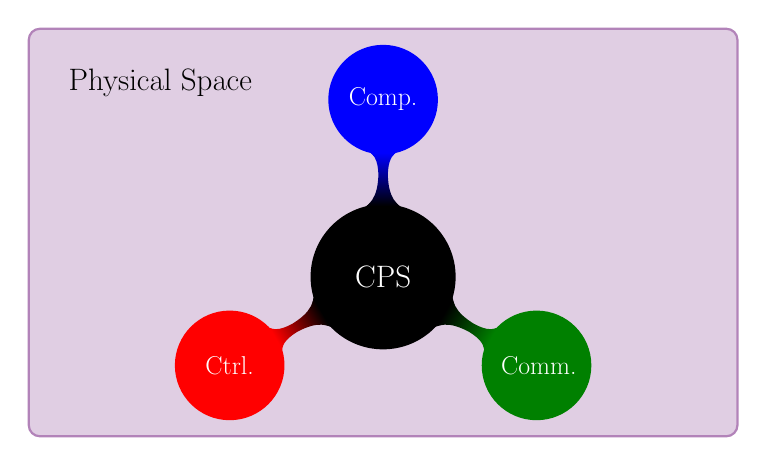
\begin{tikzpicture}[scale=0.45,transform shape,level distance=0cm,
	  level 1 concept/.append style={sibling angle=120,minimum size = 3cm},
	  ]
	  \path [draw=thupurple!50,fill=thupurple!20,thick,rounded corners] (-10,-4.5) rectangle (10,7);
	  \node at (-9,6) [anchor=north west] {\Huge Physical Space};
	  \path[mindmap,concept color=black,text=white]
	    node[concept] {\Huge CPS}
	    [clockwise from=330]
	    child[concept color=green!50!black] { node[concept](communication) {\huge Comm.} }
	    child[concept color=red] { node[concept](control) {\huge Ctrl.} }
	    child[concept color=blue] { node[concept](computation) {\huge Comp.} };
	\end{tikzpicture}
      \end{center}
    \item Applications: aerospace, chemical processes, civil infrastructure, energy, manufacturing and transportation. 
  \end{itemize}
\end{frame}

\begin{frame}{Security Threats for the CPS}
  \begin{itemize}
    \item The next generation CPS: Smart Grids, Smart Buildings, Smart Home, Internet of Things, will make extensive use of widespread sensing and networking.
    \item As the CPSs become ``smarter'', they are also more vulnerable to malicious attacks.
  \end{itemize}
  \begin{figure}[ht]
    \centering
    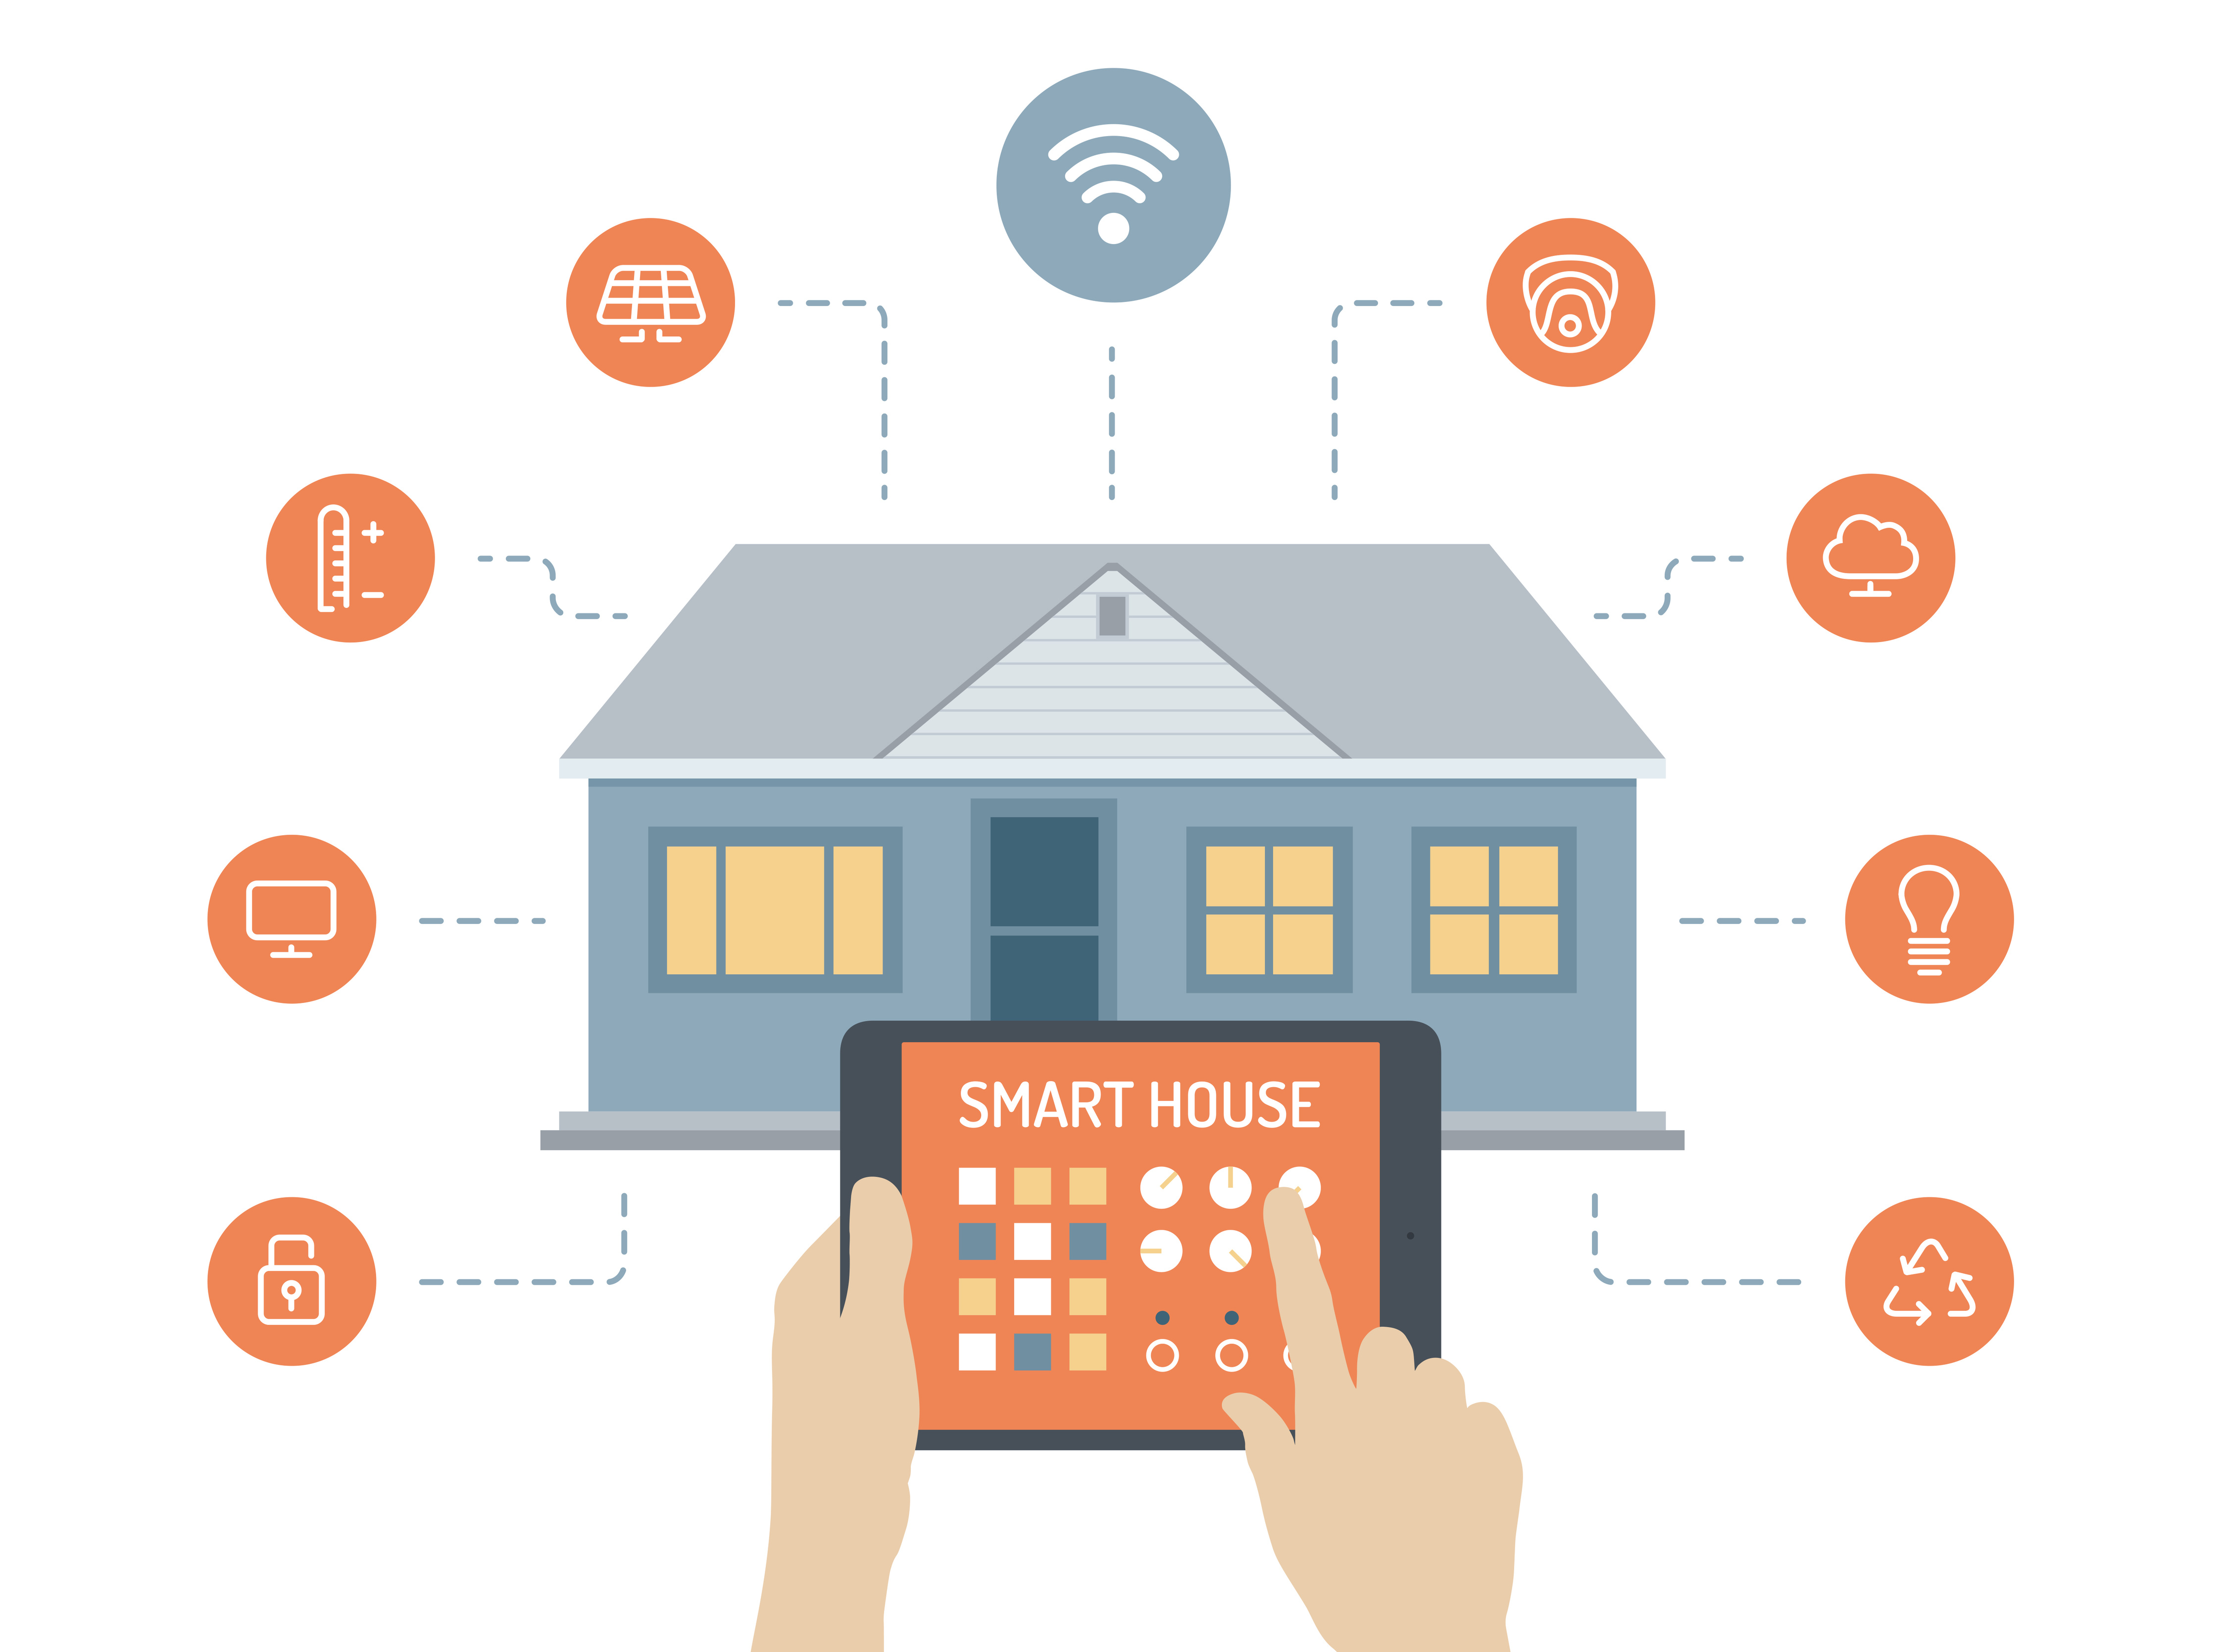
\includegraphics[width=0.6\textwidth]{SmartHome.jpg}
  \end{figure}
\end{frame}

\begin{frame}{Stuxnet}
  \begin{figure}[ht]
    \centering
    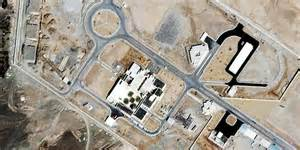
\includegraphics[width=0.8\textwidth]{stuxnet.jpg}
  \end{figure}
  Stuxnet is the first discovered malware that spies on and subverts industrial control systems. It was discovered in June 2010. 
\end{frame}

\begin{frame}{2015 Ukraine Power Outage}
  \begin{figure}[<+htpb+>]
    \begin{center}
      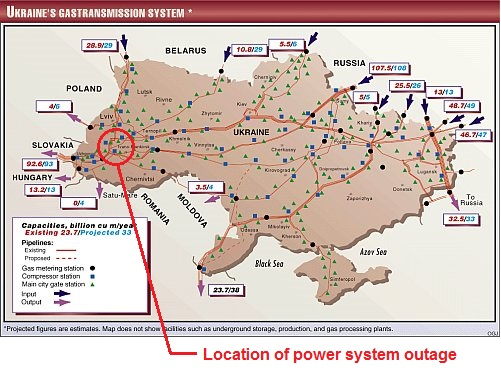
\includegraphics[width=0.60\textwidth]{ukraine.jpg}
      \caption{A successful attack on CPS can have devastating effects.}
    \end{center}
  \end{figure}
\end{frame}

\begin{frame}{Industrial Control Systems}
  \begin{figure}[ht]
    \centering
    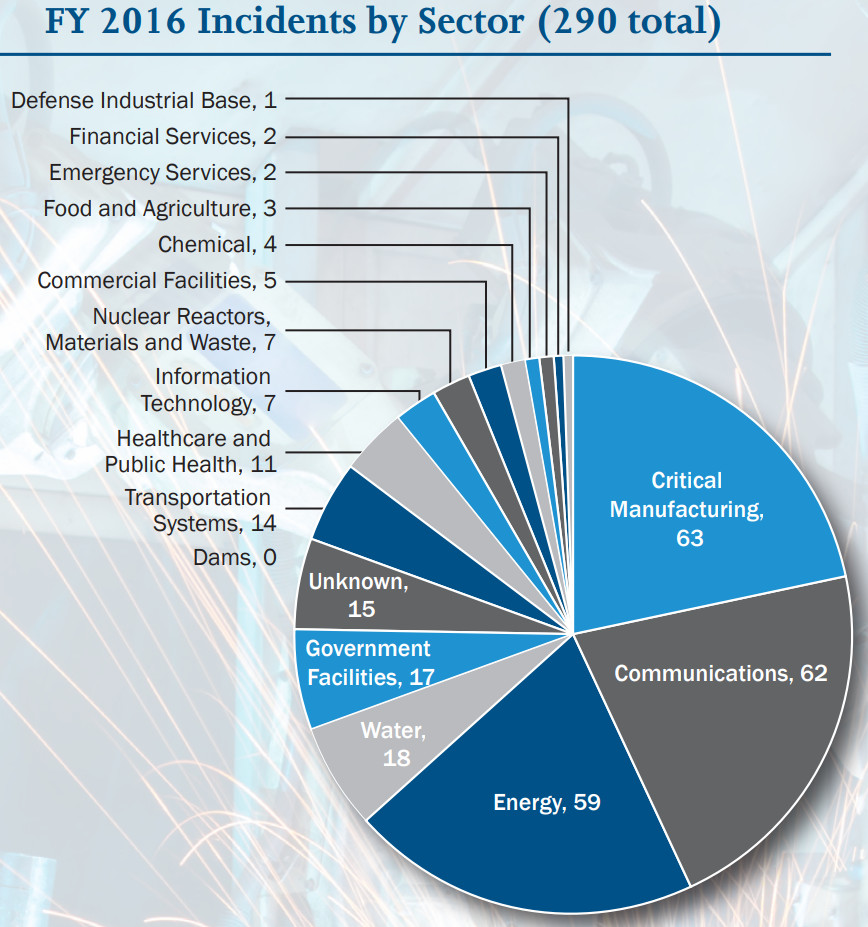
\includegraphics[width=0.55\textwidth]{cert.jpg}
  \end{figure}
  In FY 2016, ICS-CERT (Industrial Control Systems Cyber Emergency Response Team) received and responded to 290 incidents as reported by asset owners and industry partners.
\end{frame}

\begin{frame}{Industrial Control Systems}
  The scope of incidents encompassed a vast range of threats and observed methods for attempting to gain access to both business and control systems infrastructure, including but not limited to the following:
  \begin{enumerate}
    \item  Unauthorized access and exploitation of Internet facing ICS/Supervisory Control and Data Acquisition (SCADA) devices,
    \item  Exploitation of zero-day vulnerabilities in control system devices and software, 
    \item  Malware infections within air-gapped control system networks,
    \item \dots
  \end{enumerate}
\end{frame}

\begin{frame}{Attack Through Compromised Supply Chain}
  \begin{figure}[ht]
    \centering
    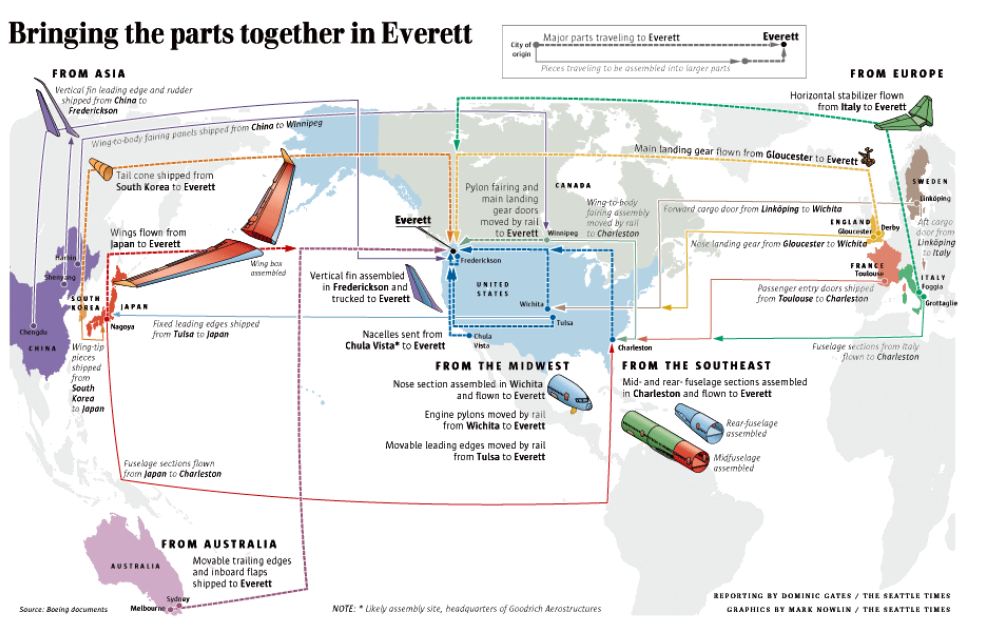
\includegraphics[width=0.8\textwidth]{boeing.jpg}
    \caption{Boeing 787 outsourced 70\% of its parts.}
  \end{figure}
\end{frame}

\begin{frame}{Hacker Taking Control of a Chrysler Jeep}
  \begin{figure}[<+htpb+>]
    \begin{center}
      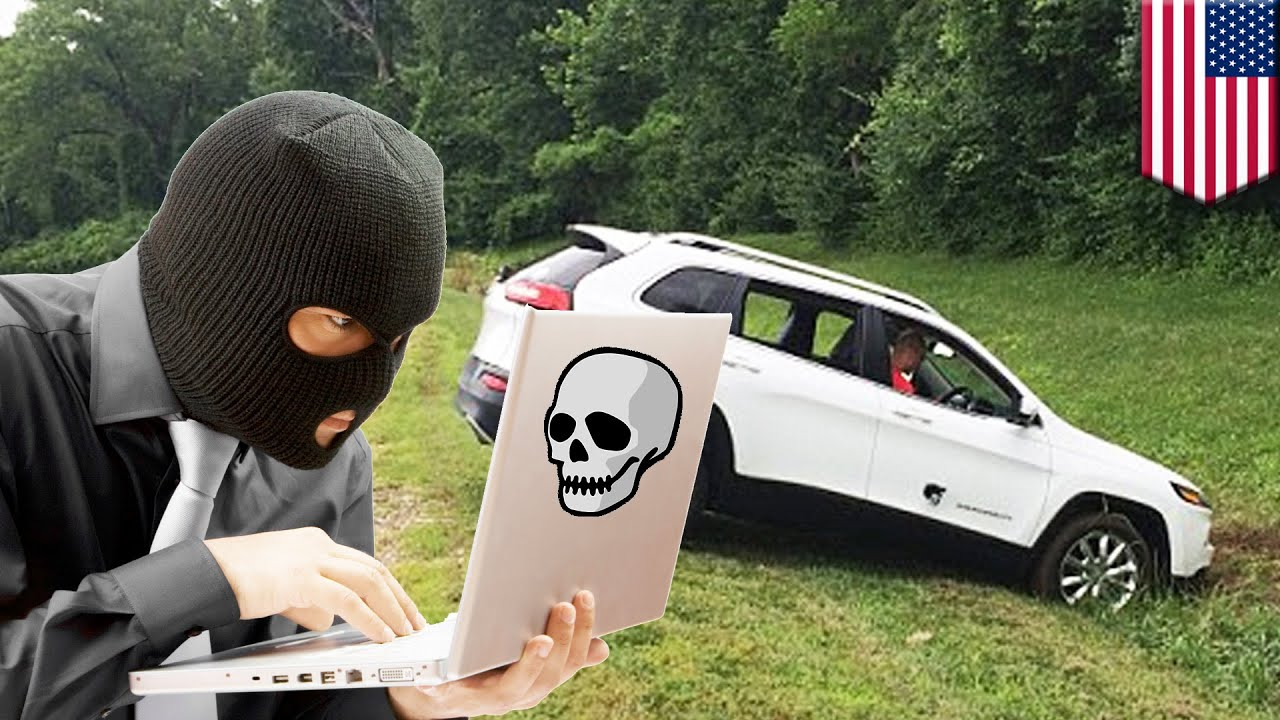
\includegraphics[width=0.80\textwidth]{jeep.jpg}
      \caption{Hacker take control of the steering and brake of a Jeep car in 2015}
    \end{center}
  \end{figure}
\end{frame}

\begin{frame}{What is New in CPS Security?}
  \begin{itemize}
    \item Physics
    \item Inertia: The system cannot be stopped at will
    \item Complicated interaction between cyber and physical world
    \item High reliability requirement: $10^{-9}$ for air plane
    \item Continuous operation, Graceful degradation.
  \end{itemize}
\end{frame}

\begin{frame}{Defense in Depth for CPS Security}
  \begin{figure}[ht]
    \centering
    \begin{tikzpicture}
      \node at (0,0) {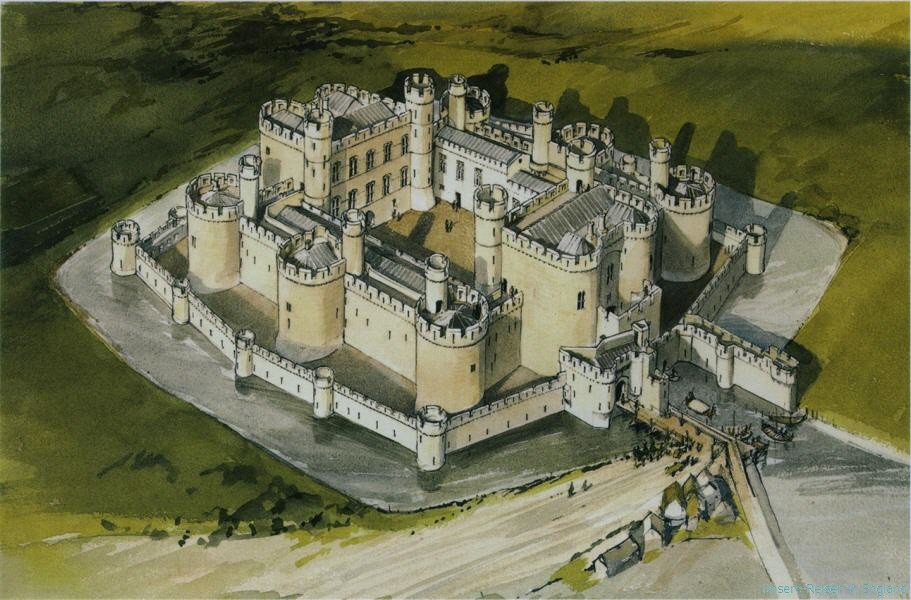
\includegraphics[width=6cm]{defense.png}};
      \node[anchor=south west] (1) at (4,1.8) {Prevention};
      \node[anchor=south west] (2) at (4,.6) {Detection};
      \node[anchor=south west] (3) at (4,-.6) {Resiliency};
      \node[anchor=south west] (4) at (4,-1.8) {Recovery};
      \draw[semithick] (2.2,0.5)--(4,1.8)--++(1.8,0);
      \draw[semithick] (2,0.4)--(4,0.6)--++(1.8,0);
      \draw[semithick] (1.2,0.6)--(4,-.6)--++(1.8,0);
      \draw[semithick] (0.2,0.7)--(4,-1.8)--++(1.8,0);
    \end{tikzpicture}
    \caption{Protecting CPS with Multi-layer Defense}
  \end{figure}
\end{frame}

\begin{frame}{What Control/System Theory Can Provide?}
  \begin{itemize}
    \item Robustness/Resiliency in off-line Design
    \item Intrusion Detection \& Isolation
    \item Secure Information Fusion/Control
    \item Security Investment
  \end{itemize}
\end{frame}

\section{Secure State Estimation}
\subsection{Static State Estimation}

\begin{frame}{Problem Formulation}
  \begin{enumerate}
    \item We assume the following sensor model:
      \begin{align*}
	\begin{bmatrix}z_1\\\vdots\\z_m\end{bmatrix} =  z = Hx + w.
      \end{align*}
    \item The optimal state estimator is of the form
      \begin{align*}
	\hat x = Kz, \text{ where }K = (H^TH)^{-1}H^T.
      \end{align*}
  \end{enumerate}
\end{frame}

\begin{frame}{Least Square Estimator}
  Suppose the following sensory model:
  \begin{align*}
    z = \begin{bmatrix}
      1\\
      1\\
      1
    \end{bmatrix}x + w.
  \end{align*}
  The optimal estimator is given by
  \begin{align*}
    \hat x = \frac{1}{3}\left(z_1+z_2+z_3\right).
  \end{align*}
  This estimator is not resilient to a single malicious sensor.
\end{frame}

\begin{frame}{Problem Formulation}
  \begin{enumerate}
    \item Assume that at most $c$ sensors are compromised.
    \item The sensory model is given by
      \begin{align*}
	y = z + a = Hx + w +a,
      \end{align*}
      where $a$ is a $c$-sparse vector indicating the attacker's action.
    \item We will call an estimator $\hat x = g(y)$ to be resilient if
      \begin{align*}
	\|g(y) - g(z)\|\text{ is bounded for all $c$-sparse $a$}.
      \end{align*}
  \end{enumerate}
\end{frame}

\begin{frame}{Some Related Research}
  \begin{enumerate}
  \item The following estimator is resilient under $2c$ observable condition:
    \begin{align*}
      & \mathop{\textit{minimize}}\limits_{\hat x,a,w}&
      & \|w\|^2 \\
      &\text{subject to}&
      &y = H \hat x + w + a,\,\|a\|_0\leq p.
    \end{align*}
  \item Difficult to verify $2c$ observable condition and difficult to solve
\item The secure estimation problem for general system is proved to be NP hard\footcite{Hendrickx2014}\footcite{Mao2019}.
  \item Can we design a secure and computationally efficient estimators for {\bf some} system?
  \end{enumerate}
\end{frame}

\begin{frame}{Example}
  Suppose the following sensory model:
  \begin{align*}
    y = \begin{bmatrix}
      1\\
      1\\
      1
    \end{bmatrix}x + w+a,\,\|a\|_0\leq 1.
  \end{align*}
  \begin{itemize}
   \item The mean is not resilient: 
  \begin{align*}
    g(y) = \argmin_{\hat x}  (y_1-\hat x)^2+(y_2-\hat x)^2+(y_3-\hat x)^2.
  \end{align*}
    \item The median is resilient to one malicious sensor.
    \item Moreover, the median can be viewed as the solution for the following optimization problem. 
  \begin{align*}
    g(y) = \argmin_{\hat x}  |y_1-\hat x|+|y_2-\hat x|+|y_3-\hat x|.
  \end{align*}
  \end{itemize}
\end{frame}

\begin{frame}{Example}
  \begin{figure}[ht]
    \centering
    \begin{tikzpicture}[yscale=0.4]
      \draw[thick,->] (0,0)--(9,0);
      \node [anchor=west] at (9,0) {$\hat x$};
      \draw[thin,gray] (2,0)--(2,0.1);
      \draw[thin,gray] (5,0)--(5,0.1);
      \draw[thin,gray] (7,0)--(7,0.1);
      \draw[thick](1,11)--(2,8)--(5,5)--(7,7)--(8,10);
      \node [anchor=north] at (2,0) {\color{red}{$y_1$}};
      \node [anchor=north] at (5,0) {\color{blue}{$y_2$}};
      \node [anchor=north] at (7,0) {\color{brown}{$y_3$}};
    \end{tikzpicture}
  \end{figure}
\end{frame}

\begin{frame}{A General Convex Optimization Based Estimator}
  We consider the following estimator
  \begin{align*}
    \hat x = g(y) \triangleq \argmin_{\hat x} \sum_{i=1}^m f_i(y_i-H_i \hat x),
  \end{align*}
  where the following properties of function $f_i:\mathbb R\mapsto \mathbb R$ are assumed:
  \begin{enumerate}
    \item $f_i$ is convex.
    \item $f_i$ is symmetric, i.e., $f_i(u) = f_i(-u)$.
    \item $f_i$ is non-negative and $f_i(0) = 0$.
  \end{enumerate} 

  Many estimators, such as least square estimator, L1 estimator and LASSO estimation can be included in this framework, by choosing a suitable $f_i$.

  The estimator can be computed efficiently via convex optimization. 
\end{frame}

\begin{frame}{A General Convex Optimization Based Estimator}
  Our proposed estimator is very general since we can choose the right $f_i$ to get the following estimator:
  \begin{enumerate}
  \item Least Square Estimator:
    \begin{align*}
      g(y) = \argmin_{\hat x} \|y-H\hat x\|_2^2= \argmin_{\hat x}  \sum_{i=1}^m (y_i-H_i\hat x)^2.
    \end{align*}
  \item $L_1$ Estimator:
    \begin{align*}
      g(y) = \argmin_{\hat x} \|y-H\hat x\|_1=\argmin_{\hat x} \sum_{i=1}^m |y_i-H_i\hat x|.
    \end{align*}
  \end{enumerate}
\end{frame}

\begin{frame}{A General Convex Optimization Based Estimator}
  \begin{enumerate}  \setcounter{enumi}{2}
  \item LASSO:
    \begin{align*}
      g(y) = \argmin_{\hat x} \|w\|^2+\gamma \|a\|_1, \text{ s.t. }y=H\hat x+w+a.
    \end{align*}
    After some manipulations, we can rewrite the optimization problem as
    \begin{align*}
      g(y) = \argmin_{\hat x} \sum_{i=1}^m f(y_i-H_i\hat x)
    \end{align*}
    where $f$ is the Huber loss function:
    \begin{align*}
      f(r) = \min_{w} w^2 + \gamma |r-w| = \begin{cases}
        r^2 & \text{if } r \leq \gamma/2\\
        \gamma |r|-\gamma^2/4 & \text{if } r\geq \gamma/2\\
      \end{cases}.
    \end{align*}
    \begin{itemize}
    \item Quadratic when the residue is small
    \item Linear when the residue is large
    \item The quadratic region is controlled by $\gamma$.
    \item We will leverage it to design an estimator that is both secure and efficient.
    \end{itemize}
  \end{enumerate}
\end{frame}

\begin{frame}{Huber Loss Function}
  \begin{figure}[ht]
    \begin{center}
      \definecolor{color0}{rgb}{0.886274509803922,0.290196078431373,0.2}
      \definecolor{color1}{rgb}{0.203921568627451,0.541176470588235,0.741176470588235}
      \setlength{\figureheight}{6cm}
      \setlength{\figurewidth}{10cm}
      % 
      \begin{tikzpicture}
	\begin{axis}[
	  width=\figurewidth,
	  height=\figureheight,
	  axis background/.style={fill=white!89.8039215686275!black},
	  axis line style={white},
	  tick align=outside,
	  tick pos=left,
	  x grid style={white},
	  xlabel={residue $r$},
	  ylabel={$f(r)$},
	  xmajorgrids,
	  xmin=-2.2, xmax=2.2,
	  xtick style={color=white!33.3333333333333!black},
	  y grid style={white},
	  ymajorgrids,
	  ymin=-0.15, ymax=3.15,
	  ytick style={color=white!33.3333333333333!black}
	  ]
	  \addplot [ultra thick, color0]
	    table[row sep=crcr]{%
	      -1 1\\
	      -0.98 0.9604\\
	      -0.96 0.9216\\
	      -0.94 0.8836\\
	      -0.92 0.8464\\
	      -0.9 0.81\\
	      -0.88 0.7744\\
	      -0.86 0.7396\\
	      -0.84 0.7056\\
	      -0.82 0.6724\\
	      -0.8 0.64\\
	      -0.78 0.6084\\
	      -0.76 0.5776\\
	      -0.74 0.5476\\
	      -0.72 0.5184\\
	      -0.7 0.49\\
	      -0.68 0.4624\\
	      -0.66 0.4356\\
	      -0.64 0.4096\\
	      -0.62 0.3844\\
	      -0.6 0.36\\
	      -0.58 0.3364\\
	      -0.56 0.3136\\
	      -0.54 0.2916\\
	      -0.52 0.2704\\
	      -0.5 0.25\\
	      -0.48 0.2304\\
	      -0.46 0.2116\\
	      -0.44 0.1936\\
	      -0.419999999999999 0.1764\\
	      -0.399999999999999 0.16\\
	      -0.379999999999999 0.1444\\
	      -0.359999999999999 0.1296\\
	      -0.339999999999999 0.1156\\
	      -0.319999999999999 0.1024\\
	      -0.299999999999999 0.0899999999999996\\
	      -0.279999999999999 0.0783999999999996\\
	      -0.259999999999999 0.0675999999999997\\
	      -0.239999999999999 0.0575999999999997\\
	      -0.219999999999999 0.0483999999999997\\
	      -0.199999999999999 0.0399999999999997\\
	      -0.179999999999999 0.0323999999999997\\
	      -0.159999999999999 0.0255999999999998\\
	      -0.139999999999999 0.0195999999999998\\
	      -0.119999999999999 0.0143999999999998\\
	      -0.0999999999999992 0.00999999999999984\\
	      -0.0799999999999992 0.00639999999999987\\
	      -0.0599999999999992 0.0035999999999999\\
	      -0.0399999999999991 0.00159999999999993\\
	      -0.0199999999999991 0.000399999999999965\\
	      8.88178419700125e-16 7.88860905221012e-31\\
	      0.0200000000000009 0.000400000000000036\\
	      0.0400000000000009 0.00160000000000007\\
	      0.0600000000000009 0.00360000000000011\\
	      0.080000000000001 0.00640000000000015\\
	      0.100000000000001 0.0100000000000002\\
	      0.120000000000001 0.0144000000000002\\
	      0.140000000000001 0.0196000000000003\\
	      0.160000000000001 0.0256000000000003\\
	      0.180000000000001 0.0324000000000004\\
	      0.200000000000001 0.0400000000000004\\
	      0.220000000000001 0.0484000000000005\\
	      0.240000000000001 0.0576000000000005\\
	      0.260000000000001 0.0676000000000006\\
	      0.280000000000001 0.0784000000000006\\
	      0.300000000000001 0.0900000000000007\\
	      0.320000000000001 0.102400000000001\\
	      0.340000000000001 0.115600000000001\\
	      0.360000000000001 0.129600000000001\\
	      0.380000000000001 0.144400000000001\\
	      0.400000000000001 0.160000000000001\\
	      0.420000000000001 0.176400000000001\\
	      0.440000000000001 0.193600000000001\\
	      0.460000000000001 0.211600000000001\\
	      0.480000000000001 0.230400000000001\\
	      0.500000000000001 0.250000000000001\\
	      0.520000000000001 0.270400000000001\\
	      0.540000000000001 0.291600000000001\\
	      0.560000000000001 0.313600000000002\\
	      0.580000000000001 0.336400000000002\\
	      0.600000000000001 0.360000000000002\\
	      0.620000000000001 0.384400000000002\\
	      0.640000000000001 0.409600000000002\\
	      0.660000000000001 0.435600000000002\\
	      0.680000000000001 0.462400000000002\\
	      0.700000000000002 0.490000000000002\\
	      0.720000000000002 0.518400000000002\\
	      0.740000000000002 0.547600000000002\\
	      0.760000000000002 0.577600000000002\\
	      0.780000000000002 0.608400000000002\\
	      0.800000000000002 0.640000000000003\\
	      0.820000000000002 0.672400000000003\\
	      0.840000000000002 0.705600000000003\\
	      0.860000000000002 0.739600000000003\\
	      0.880000000000002 0.774400000000003\\
	      0.900000000000002 0.810000000000003\\
	      0.920000000000002 0.846400000000003\\
	      0.940000000000002 0.883600000000003\\
	      0.960000000000002 0.921600000000003\\
	      0.980000000000002 0.960400000000003\\
	      1 1\\
	    };
	    \addplot [ultra thick, color1]
	    table[row sep=crcr] {%
	      1 1\\
	      1.5 2\\
	      2 3\\
	    };
	    \addplot [ultra thick, color1]
	    table[row sep=crcr] {%
	      -1 1\\
	      -1.5 2\\
	      -2 3\\
	    };
	  \end{axis}
	\end{tikzpicture}%
      \end{center}
    \end{figure}


\end{frame}


\begin{frame}{Example}
  Going back to the previous example:
  \begin{align*}
    y = \begin{bmatrix}
      1\\
      1\\
      1
    \end{bmatrix}x + w+a,\,\|a\|_0\leq 1.
  \end{align*}
  The median is the solution of:
  \begin{align*}
    g(y) = \argmin_{\hat x}  |y_1-\hat x|+|y_2-\hat x|+|y_3-\hat x|.
  \end{align*}

  \begin{figure}[ht]
    \centering
    \begin{tikzpicture}[yscale=0.4]
      \draw[thick,->] (0,2)--(9,2);
      \node [anchor=west] at (9,2) {$\hat x$};
      \draw[thin,gray] (2,0)--(2,0.1);
      \draw[thin,gray] (5,0)--(5,0.1);
      \draw[thin,gray] (7,0)--(7,0.1);
      \draw[thick](1,11)--(2,8)--(5,5)--(7,7)--(8,10);
      \node [anchor=north] at (2,2) {\color{red}{$y_1$}};
      \node [anchor=north] at (5,2) {\color{blue}{$y_2$}};
      \node [anchor=north] at (7,2) {\color{brown}{$y_3$}};
    \end{tikzpicture}
  \end{figure}
\end{frame}

\begin{frame}{Interpretation}
  \begin{figure}[ht]
    \centering
    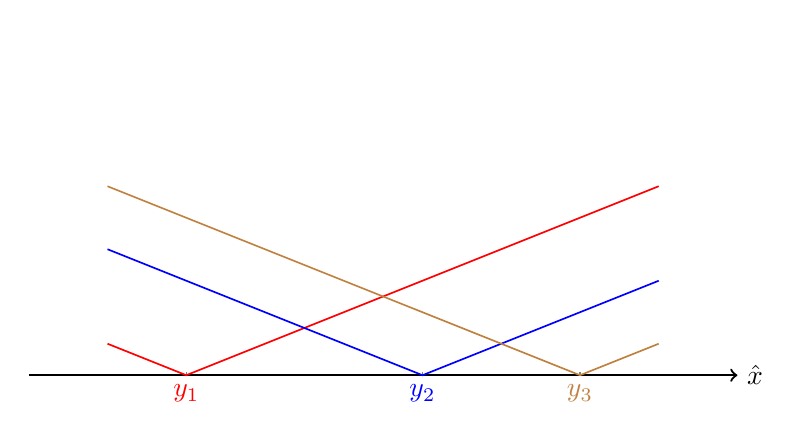
\begin{tikzpicture}[yscale=0.4]
      \draw[thick,->] (0,0)--(9,0);
      \node [anchor=west] at (9,0) {$\hat x$};
      \draw[thin,gray] (2,0)--(2,0.1);
      \draw[thin,gray] (5,0)--(5,0.1);
      \draw[thin,gray] (7,0)--(7,0.1);
      \draw[thick,white](1,11)--(2,8)--(5,5)--(7,7)--(8,10);
      \node [anchor=north] at (2,0) {\color{red}{$y_1$}};
      \draw[semithick,red](1,1)--(2,0)--(8,6);
      \node [anchor=north] at (5,0) {\color{blue}{$y_2$}};
      \draw[semithick,blue](1,4)--(5,0)--(8,3);
      \node [anchor=north] at (7,0) {\color{brown}{$y_3$}};
      \draw[semithick,brown](1,6)--(7,0)--(8,1);
    \end{tikzpicture}
  \end{figure}
  If we interpret the function $|y_i-\hat x|$ as a potential function generate by sensor $i$, then we can see that sensor $i$ is dragging $\hat x$ towards $y_i$ with $1$ unit of force. The equilibrium point will be at the middle $y_i$.
\end{frame}

\begin{frame}{Another Example}
  Suppose the following sensory model:
  \begin{align*}
    y = \begin{bmatrix}
      1\\
      1\\
      3
    \end{bmatrix}x + w+a ,\,\|a\|_0\leq 1.
  \end{align*}
  Then the following estimator is not resilient:
  \begin{align*}
    g(y) = \argmin_{\hat x}  |y_1-\hat x|+|y_2-\hat x|+|y_3-3\hat x|.
  \end{align*}
  In fact, we can rewrite it as
  \begin{align*}
    g(y) = \argmin_{\hat x}  |y_1-\hat x|+|y_2-\hat x|+3\left|\frac{y_3}{3}-\hat x\right| = \frac{y_3}{3}
  \end{align*}
  Sensor $3$ generates $3$ unit of force comparing to $1$ unit of force from sensor $1$ and $2$.
\end{frame}

\begin{frame}{Sufficient Condition For Resiliency}
  \begin{theorem}
    If the following conditions hold, then the estimation is resilient:
    \begin{enumerate}
      \item For all $i$, the following limit is well-defined:
	\begin{align*}
	  \lim_{t\rightarrow\infty}\frac{f_i(tH_iu)}{t} = C_i(u) < \infty.
	\end{align*}
      \item For any $u\neq 0$ and any index set $\mathcal I$ of cardinality $c$, the following inequality hold:
	\begin{align*}
	  \sum_{i\in \mathcal I} C_i(u) < \sum_{i\in \mathcal I^c} C_i(u). 
	\end{align*}
    \end{enumerate}
  \end{theorem}
  Roughly speaking $C_i(u)$ characterize how powerful a single sensor $i$ is along direction $u$. The condition can be interpreted as the no $c$ sensors combined can be more powerful than the remaining $m-c$ sensors.
\end{frame}

\begin{frame}{Necessary Condition For Resiliency}
  \begin{theorem}
    If the one of the following conditions is violated, then the estimation is not resilient:
    \begin{enumerate}
      \item There exists an $i$ and $u$, such that
	\begin{align*}
 \lim_{t\rightarrow\infty}\frac{f_i(tH_iu)}{t} = \infty.
	\end{align*}
      \item There exists a $u\neq 0$ and an index set $\mathcal I$ of cardinality $c$, such that
	\begin{align*}
	  \sum_{i\in \mathcal I} C_i(u) > \sum_{i\in \mathcal I^c} C_i(u). 
	\end{align*}
    \end{enumerate}
  \end{theorem}
  Notice that we only have a trivial gap for the case:
\begin{align*}
  \sum_{i\in \mathcal I} C_i(u) = \sum_{i\in \mathcal I^c} C_i(u).
\end{align*}	  
\end{frame}

\begin{frame}{In Summary\footcite{Han2019}}
  \begin{itemize}
    \item We design a convex optimization based estimator
  \begin{align*}
    \hat x = g(y) \triangleq \argmin_{\hat x} \sum_{i=1}^m f_i(y_i-H_i \hat x).
  \end{align*}
    \item Difficult to verify the resiliency condition
      \begin{align*}
	\sum_{i\in \mathcal I} C_i(u) < \sum_{i\in \mathcal I^c} C_i(u). 
      \end{align*}
    \item Easy to compute via convex optimization
    \item If $f_i$ is the Huber loss function, then we could recover the least square estimate if:
      \begin{itemize}
	\item there is no attack
	\item the noise is "small"
      \end{itemize}
  \end{itemize}
\end{frame}

\begin{frame}{Simulation IEEE 14-bus System}
  \begin{figure}[ht]
    \centering
    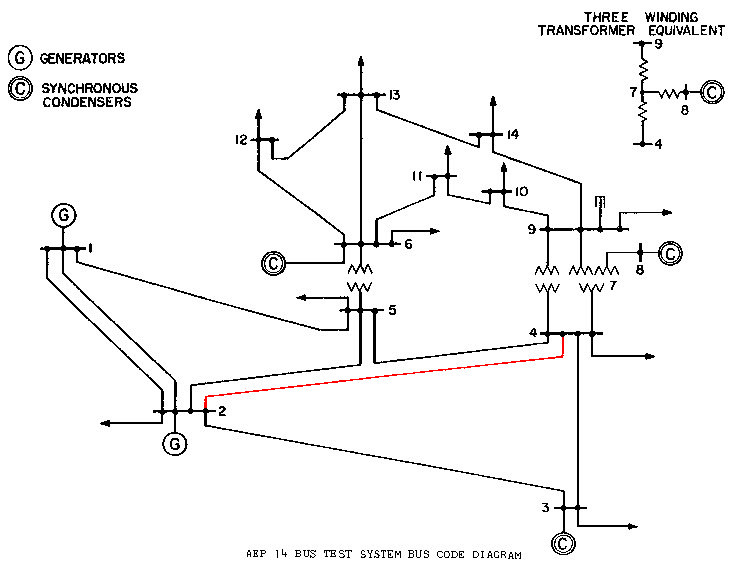
\includegraphics[width=0.60\textwidth]{ieee14.jpg}
  \end{figure}
  We assume $c=1$ and the flow sensor on the red line is being attacked.
\end{frame}

\begin{frame}{Simulation IEEE 14-bus System}
  \begin{figure}[ht]
    \begin{center}

      \setlength{\figureheight}{6cm}
      \setlength{\figurewidth}{10cm}
      \definecolor{mycolor1}{rgb}{1.00000,0.00000,1.00000}%
      % 
      \begin{tikzpicture}

	\begin{axis}[%
	  width=\figurewidth,
	  height=\figureheight,
	  at={(1.527in,1.083in)},
	  scale only axis,
	  xmin=0.95,
	  xmax=2.4,
	  xlabel={Normalized MSE of the estimators without attack},
	  xmajorgrids,
	  ymin=0.95,
	  ymax=2.5,
	  ylabel={Normalized MSE when under attack},
	  ymajorgrids,
	  axis background/.style={fill=white},
	  legend style={at={(0.597,0.528)},anchor=south west,legend cell align=left,align=left,draw=white!15!black}
	  ]
	  \addplot [color=blue,dashed,line width=1.5pt,mark=triangle,mark options={solid},forget plot]
	    table[row sep=crcr]{%
	      2.16434829886514	2.41673714136766\\
	      1.49824142620916	1.6273922047888\\
	      1.46836558726546	1.61304395019434\\
	      1.42878218405531	1.58080265845186\\
	      1.33509034059386	1.48317348510781\\
	      1.24979953097586	1.4011442907391\\
	      1.20190884155895	1.36475282176979\\
	      1.14816845697376	1.32743887772808\\
	      1.104692902235	1.30458587111275\\
	      1.0727554366346	1.2930587844785\\
	      1.04837293442887	1.29286647088633\\
	      1.03276380632143	1.30464750437787\\
	      1.02491383863213	1.32636243694814\\
	      1.0209295289153	1.35606289076979\\
	      1.01470702949196	1.40680155569416\\
	      1.00686189169388	1.48274325705327\\
	      1.00166658882151	1.69020329692052\\
	      1.00012894457222	2.29806950301701\\
	    };

	  \addplot [color=mycolor1,dashed,forget plot]
	    table[row sep=crcr]{%
	      1	1\\
	      2.2	1\\
	    };
	  \addplot [color=mycolor1,dashed,forget plot]
	    table[row sep=crcr]{%
	      1	1\\
	      1	2.5\\
	    };
	  \node[right, align=left, text=blue]
	  at (axis cs:2.164,2.417) {$\text{   }\leftarrow\text{ }\gamma\rightarrow 0$};
	  \node[right, align=left, text=blue]
	  at (axis cs:1.335,1.483) {$\text{   }\leftarrow\text{ }\gamma\text{=0.5}$};
	  \node[right, align=left, text=blue]
	  at (axis cs:1.202,1.365) {$\text{   }\leftarrow\text{ }\gamma\text{=1}$};
	  \node[right, align=left, text=blue]
	  at (axis cs:1.073,1.293) {$\text{   }\leftarrow\text{ }\gamma\text{=1.9}$};
	  \node[right, align=left, text=blue]
	  at (axis cs:1.02,1.356) {$\leftarrow\gamma\text{=3}$};
	  \node[right, align=left, text=blue]
	  at (axis cs:1,2.298) {$\text{   }\leftarrow\text{ }\gamma\text{=7}$};
	  \node[right, align=left, text=mycolor1]
	  at (axis cs:1,2.4) {$\text{   }\leftarrow\text{ LSE}$};
	  \node[right, align=left, text=mycolor1]
	  at (axis cs:1.9,1.14) {Oracle LSE};
	  \node[right, align=left, text=mycolor1]
	  at (axis cs:1.9,1.07) {$\text{     ~~~~~}\downarrow$};
	\end{axis}
      \end{tikzpicture}%
    \end{center}
  \end{figure}
\end{frame}

\subsection{Dynamic State Estimation}
\begin{frame}{Dynamic State Estimation}
  \begin{enumerate}
    \item Consider the following dynamic system
      \begin{align}
	x(k+1) = A x(k) + w(k),\, y(k) = C x(k) + v(k) + a(k).
      \end{align}
    \item A linear fixed-gain estimator:
      \begin{align}
	\hat x(k+1) = A \hat x(k) + K(y(k+1)-CA\hat x(k)),
      \end{align}
      where $K$ is the estimation gain, and $A-KCA$ is stable.
      \begin{center}
	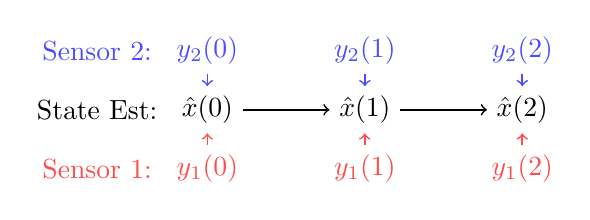
\begin{tikzpicture}[x=2cm, y=0.75cm]
	  \node at (-0.7,0) {State Est:};
	  \node [blue!70] at (-0.7,1) {Sensor 2:};
	  \node [red!70] at (-0.7,-1) {Sensor 1:};

	  \node            (x0)  at (0,0) {$\hat x(0)$};
	  \node [blue!70] (y20)  at (0,1)    {$y_2(0)$};
	  \node [red!70]  (y10)  at (0,-1)   {$y_1(0)$};
	  \draw [->,semithick,blue!70] (y20) to (x0);
	  \draw [->,semithick,red!70]  (y10) to (x0);

	  \node            (x1)  at (1,0) {$\hat x(1)$};
	  \node [blue!70] (y21)  at (1,1)    {$y_2(1)$};
	  \node [red!70]  (y11)  at (1,-1)   {$y_1(1)$};
	  \draw [->,semithick,blue!70] (y21) to (x1);
	  \draw [->,semithick,red!70]  (y11) to (x1);

	  \node            (x2)  at (2,0) {$\hat x(2)$};
	  \node [blue!70] (y22)  at (2,1)    {$y_2(2)$};
	  \node [red!70]  (y12)  at (2,-1)   {$y_1(2)$};
	  \draw [->,semithick,blue!70] (y22) to (x2);
	  \draw [->,semithick,red!70]  (y12) to (x2);

	  \draw [->,semithick] (x0) to (x1);
	  \draw [->,semithick] (x1) to (x2);
	\end{tikzpicture}
      \end{center}
    \item Captures most of the estimators: steady-state Kalman filter, $H_2$/$H_\infty$ estimator
    \item The error introduced by the attack may accumulate over time.
  \end{enumerate}
\end{frame}

\begin{frame}{Fundamental Limit}
  If the system becomes undetectable after removing $2c$ sensors, then there exists an attack on $c$ sensors, such that NO estimator can have bounded estimation error \footcite{Nakahira2018}.
\end{frame}

\begin{frame}{Dynamic State Estimate: A Moving Horizon Approach}
In order to convert the dynamic estimation problem into a static one, we can use a moving horizon approach\footcite{Fawzi2014}\footcite{Shoukry2017}:
  \begin{center}
    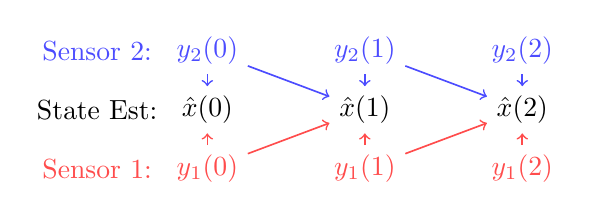
\begin{tikzpicture}[x=2cm, y=0.75cm]
      \node at (-0.7,0) {State Est:};
      \node [blue!70] at (-0.7,1) {Sensor 2:};
      \node [red!70] at (-0.7,-1) {Sensor 1:};

      \node            (x0)  at (0,0) {$\hat x(0)$};
      \node [blue!70] (y20)  at (0,1)    {$y_2(0)$};
      \node [red!70]  (y10)  at (0,-1)   {$y_1(0)$};
      \draw [->,semithick,blue!70] (y20) to (x0);
      \draw [->,semithick,red!70]  (y10) to (x0);

      \node            (x1)  at (1,0) {$\hat x(1)$};
      \node [blue!70] (y21)  at (1,1)    {$y_2(1)$};
      \node [red!70]  (y11)  at (1,-1)   {$y_1(1)$};
      \draw [->,semithick,blue!70] (y21) to (x1);
      \draw [->,semithick,red!70]  (y11) to (x1);
      \draw [->,semithick,blue!70] (y20) to (x1);
      \draw [->,semithick,red!70]  (y10) to (x1);

      \node            (x2)  at (2,0) {$\hat x(2)$};
      \node [blue!70] (y22)  at (2,1)    {$y_2(2)$};
      \node [red!70]  (y12)  at (2,-1)   {$y_1(2)$};
      \draw [->,semithick,blue!70] (y22) to (x2);
      \draw [->,semithick,red!70]  (y12) to (x2);
      \draw [->,semithick,blue!70] (y21) to (x2);
      \draw [->,semithick,red!70]  (y11) to (x2);
    \end{tikzpicture}
  \end{center}

  However, the historical data are discarded and the estimation performance may be poor when the system is operating normally.
\end{frame}

\begin{frame}{Dynamic State Estimate: A Local Estimator Approach}
  We propose to store historical data in the local estimations:
  \begin{center}
    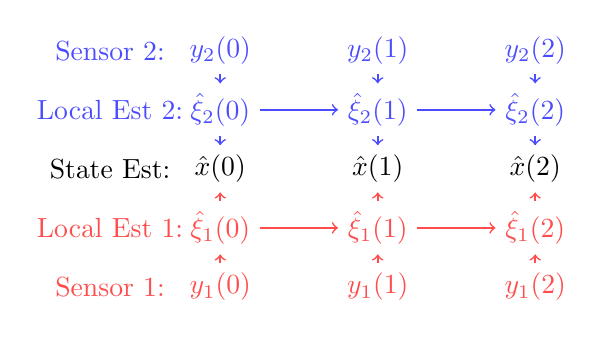
\begin{tikzpicture}[x=2cm, y=0.75cm]
      \node at (-0.7,0) {State Est:};
      \node [blue!70] at (-0.7,2) {Sensor 2:};
      \node [blue!70] at (-0.7,1) {Local Est 2:};
      \node [red!70] at (-0.7,-2) {Sensor 1:};
      \node [red!70] at (-0.7,-1) {Local Est 1:};

      \node            (x0)  at (0,0)    {$\hat x(0)$};
      \node [blue!70] (y20)  at (0,2)       {$y_2(0)$};
      \node [blue!70] (x20)  at (0,1)  {$\hat \xi_2(0)$};
      \node [red!70]  (y10)  at (0,-2)      {$y_1(0)$};
      \node [red!70]  (x10)  at (0,-1) {$\hat \xi_1(0)$};
      \draw [->,semithick,blue!70] (y20) to (x20);
      \draw [->,semithick,red!70]  (y10) to (x10);
      \draw [->,semithick,blue!70] (x20) to  (x0);
      \draw [->,semithick,red!70]  (x10) to  (x0);

      \node            (x1)  at (1,0)    {$\hat x(1)$};
      \node [blue!70] (y21)  at (1,2)       {$y_2(1)$};
      \node [blue!70] (x21)  at (1,1)  {$\hat \xi_2(1)$};
      \node [red!70]  (y11)  at (1,-2)      {$y_1(1)$};
      \node [red!70]  (x11)  at (1,-1) {$\hat \xi_1(1)$};
      \draw [->,semithick,blue!70] (y21) to (x21);
      \draw [->,semithick,red!70]  (y11) to (x11);
      \draw [->,semithick,blue!70] (x21) to  (x1);
      \draw [->,semithick,red!70]  (x11) to  (x1);

      \node            (x2)  at (2,0)    {$\hat x(2)$};
      \node [blue!70] (y22)  at (2,2)       {$y_2(2)$};
      \node [blue!70] (x22)  at (2,1)  {$\hat \xi_2(2)$};
      \node [red!70]  (y12)  at (2,-2)      {$y_1(2)$};
      \node [red!70]  (x12)  at (2,-1) {$\hat \xi_1(2)$};
      \draw [->,semithick,blue!70] (y22) to (x22);
      \draw [->,semithick,red!70]  (y12) to (x12);
      \draw [->,semithick,blue!70] (x22) to  (x2);
      \draw [->,semithick,red!70]  (x12) to  (x2);

      \draw [->,semithick,blue!70] (x20) to (x21);
      \draw [->,semithick,blue!70] (x21) to (x22);
      \draw [->,semithick,red!70] (x10) to (x11);
      \draw [->,semithick,red!70] (x11) to (x12);
    \end{tikzpicture}
  \end{center}
  \begin{enumerate}
    \item Construct local estimators for each sensor (which uses only the local measurements)
    \item Reconstruct the global estimator 
  \end{enumerate}
\end{frame}

%\begin{frame}{Local Estimator Design}
%  \begin{enumerate}
%    \item  Choose $L_i$ such that $A-L_iCA$ shares the same eigenvalues as $A-KCA$ (requires observability)
%      \begin{align*}
%	\hat x_i(k) = A \hat x_i(k) + L_i (y_i(k)-CA\hat x_i(k)).
%      \end{align*}  
%    \item The global estimate can be recovered as
%      \begin{align*}
%	\hat x(k) = F_1\hat x_1(k)+\dots+F_m\hat x_m(k).
%      \end{align*}
%    \item More importantly, it can be written as the solution of a quadratic programming problem:
%      \begin{align*}
%      &\mathop{\textrm{minimize}}\limits_{\hat x(k),\hat e(k)}&
%      & \frac{1}{2}\hat e(k)^T \tilde W^{-1} \hat e(k)\\
%      &\textrm{subject to} &
%      &\hat x_i(k)  =  \hat x(k) + \hat e_i(k),&
%      \end{align*}
%  \end{enumerate}
%\end{frame}

\begin{frame}{Local Estimator Design}
  We make the following assumptions:
  \begin{enumerate}
    \item The system $(A,C)$ is observable. However the whole state space may not be observable for individual sensors.  
    \item The eigenvalues of $A-KCA$ are distinct.   
    \item $A-KCA$ do not share eigenvalues with $A$.
  \end{enumerate}
  As a result, we could design the estimator as:
  \begin{align*}
    \hat \xi_i(k) = \Lambda \hat \xi_i(k) + \mathbf 1 y_i(k+1), 
  \end{align*}  
  where
  \begin{enumerate}
    \item $\Lambda = diag (\lambda_1, \ldots, \lambda_n)$ is a diagonal matrix, such that $A-KCA = V\Lambda V^{-1}.$
      \item $\mathbf 1$ is an all-one vector of dimension $n$.
  \end{enumerate}
\end{frame}

\begin{frame}{Properties of the Local Estimator in the Absence of Attack}
  \begin{enumerate}
    \item $\hat \xi_i$ is a stable estimate of $G_ix$, where
      \begin{align*}
	G_{i} \triangleq
	\begin{bmatrix}
	  C_{i} A\left(A-\lambda_{1} I\right)^{-1} \\
	  \vdots \\
	  C_{i} A\left(A-\lambda_{n} I\right)^{-1}
	\end{bmatrix}.
      \end{align*}
    \item The null space of $G_i$ matrix is exactly the unobservable state space for sensor $i$.
    \item  The estimation error $\epsilon_i(k)\triangleq G_i x(k)-\xi_i(k)$ follows:
      \begin{align*}
	\epsilon_{i}(k+1)= \Lambda \epsilon_{i}(k)+\left(G_{i}-\mathbf{1} C_{i}\right) w(k) -\mathbf{1} v_{i}(k+1).
      \end{align*}
    \item The Kalman estimate can be recovered as the solution of a least square problem:
      \begin{align*}
      &\mathop{\textrm{minimize}}\limits_{\hat x(k),\hat \epsilon(k)}&
      & \frac{1}{2}\hat \epsilon(k)^T \tilde W^{-1} \hat \epsilon(k)\\
      &\textrm{subject to} &
      &\hat \xi_i(k)  =  G_i\hat x(k) + \hat \epsilon_i(k),&
      \end{align*}
      where the matrix $\tilde W$ is the asymptotic covariance of $[\epsilon_1^T,\ldots ,\epsilon_n^T]$.
  \end{enumerate}
\end{frame}

\begin{frame}{Securing the Global Estimate with LASSO}
  \begin{itemize}
    \item  In the presence of attack, the estimation error follows:
      \begin{align*}
	\epsilon_{i}(k+1)= \Lambda \epsilon_{i}(k)+\left(G_{i}-\mathbf{1} C_{i}\right) w(k) -\mathbf{1} v_{i}(k+1) - \mathbf{1} a_{i}(k+1) .
      \end{align*}
    \item We can secure the global estimator using LASSO:
      \begin{align*}
    &\mathop{\textrm{minimize}}\limits_{\hat x(k),\hat \epsilon(k), \hat \nu(k)}&
    & \frac{1}{2}\hat \epsilon(k)^T \tilde W^{-1} \hat \epsilon(k) + \gamma \sum_{i=1}^m \|\hat \nu_i(k)\|_1\\
    &\textrm{subject to} &
    &\hat \xi_i(k)  =  G_i\hat x(k) + \hat \epsilon_i(k)+\hat \nu_i(k).&
      \end{align*}
  \end{itemize}
\end{frame}

\begin{frame}{Efficiency and Security\footcite{Liu2017}}
  \begin{block}{Efficiency}
    \begin{itemize}
      \item In the absence of attack, we recover the Kalman estimate if the noise is "small".
      \item Given a probability $p<1$, we can tune $\gamma$ such that we recover KF with probability $p$.
    \end{itemize}
  \end{block}
  \begin{block}{Security}
    In the presence of attack, the estimator is stable if for any $u\neq 0$ and any index set $\mathcal I$ of cardinality $c$, the following inequality hold:
    \begin{align*}
      \sum_{i\in \mathcal I} \|G_iu\|_1 < \sum_{i\in \mathcal I^c} \|G_iu\|_1. 
    \end{align*}
  \end{block}
\end{frame}

\begin{frame}{The Last Piece of the Puzzle\footcite{Mao2019}}
  \begin{itemize}
    \item Consider a $2$-dimensional system with $A = diag(1,2)$ 
    \item The observable space for a sensor can only be $\{x_1\},\,\{x_2\}$ or $\{x_1,\,x_2\}$
    \item It is not possible for the observable space to be $\{ax_1+bx_2\}$ with non-zero $a,b$!
    \item As such, we could always transform $G_i$ into
      \begin{align*}
	G_i = \begin{bmatrix}
	  1&0\\
	  0&0
	  \end{bmatrix} ,\,\begin{bmatrix}
	  0&1\\
	  0&0
	  \end{bmatrix} ,\,or\,\begin{bmatrix}
	  1&0\\
	  0&1
	\end{bmatrix} .
      \end{align*}
  \end{itemize}
\end{frame}

\begin{frame}{In Summary}
  Given a probability $p<1$, if all unstable eigenvalues of the system matrix $A$ has geometric multiplicity of $1$, then we can design an estimator, such that
  \begin{enumerate}
    \item Close to optimal {\bf efficiency}: In the absence of attack, the estimator coincides with the optimal Kalman estimator with probability $p$.
    \item Optimal {\bf security}: The estimator is resilient against $c$ malicious sensors, assuming that every unstable state can be observed by at least $2c+1$ sensors.
  \end{enumerate}
  It is easy to certify the security of the estimator and compute the state estimate in real time. 
\end{frame}

\begin{frame}{Distributed secure estimation}
	The estimation can be done on a digraph in distributed manner in \textbf{bounded noise case}. At each time step $k$, each sensor $i$ do the following 3 steps:
	\begin{enumerate}
		\item Calculate local estimation $\hat{\xi}_i$.
		\item Malicious detection $\|\hat{\xi}_i(k)-G_i x(k)\|\geq \bar{\gamma}$.
		\item Do $T$ times of optimization iterations:
		\begin{itemize}
			\item For benign sensors (consensus+prox-grad descent):
			\begin{align*}
				\cx_i^{(t+1)}=& \cx_i^{(t)}-\beta u_i^{(t)}-\frac{\beta \alpha}{|\Nc_i|}\sum_{j\in\Nc_i} \left[\cx_i^{(t)} -\cx_j^{(t)}\right] - \beta  \left(\text{prox-grad term}\right)\\
				u_i^{(t+1)}=&u_i^{(t)}+\frac{\omega}{|\Nc_i|}\sum_{j\in\Nc_i} \left[\cx_i^{(t+1)} -\cx_j^{(t+1)}\right]. 
			\end{align*}
			\item For Malicious sensors (only consensus): 
			\begin{align*}
				\cx_i^{(t+1)}=& \cx_i^{(t)}-\beta u_i^{(t)}-\frac{\beta \alpha}{|\Nc_i|}\sum_{j\in\Nc_i} \left[\cx_i^{(t)} -\cx_j^{(t)}\right]\\
				u_i^{(t+1)}=&u_i^{(t)}+\frac{\omega}{|\Nc_i|}\sum_{j\in\Nc_i} \left[\cx_i^{(t+1)} -\cx_j^{(t+1)}\right]. \hspace{85pt}
			\end{align*}
	\end{itemize}
	\end{enumerate}

\end{frame}

\begin{frame}{Distributed secure estimation}

	\begin{block}{Theorem}
	In the presence of attack, if the previous security condition is satisfied, for arbitrary $\delta>0$, by choosing iteration number $T$ and detector threshold $\gamma$ as 
	\begin{align}
		T&\geq -2\log_{\rho}\left[ \frac{1}{\delta} \left( \|A\|_2(\delta+\Bc_{*})+\Bc_{w}+ \Bc_{*} \right)\right], \label{eq:chooseT}\\
		\gamma&\triangleq\Bc_\epsilon + \left\|G_i\right\|_2 (\delta+\Bc_{*}), \label{eq:choose_gamma}
	\end{align}
	in Algorithm where $0<\rho<1$ is the linear convergence rate, the estimation error of our proposed algorithm is
	\begin{align*}
		\left\|\cx_i^{(T)}(k)-x(k)\right\|_2 \leq \Bc_{*}+\delta, \ \forall i\in\Ica, k\in\Nb,
	\end{align*}
	Moreover, benign sensors do not trigger the malicious detector.
	
	\end{block}


	
\end{frame}

\begin{frame}{Numerical Example: 6 agent system}
	\begin{columns}
		\begin{column}{0.5\textwidth}
				\begin{align*}
				A=\begin{bmatrix}
					1.1  &   1  &  0\\
					0 & 1.1  &    0\\
					0  &   0  &  0.9
				\end{bmatrix},\  C=
				\begin{bmatrix}
					1 &0& 0\\
					0& 1& 0\\
					1& 1& 0\\
					0 &1& 1\\
					1& 0& 1\\
					0 &0& 1
				\end{bmatrix}.
			\end{align*}
		\end{column}
	\begin{column}{0.5\textwidth}
		\begin{figure}[htpb!]
			\centering
			

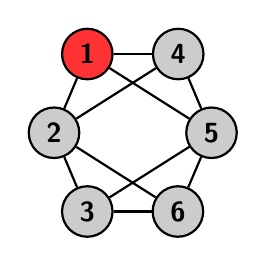
\begin{tikzpicture}[-, thick,main node/.style={circle,draw,fill=black!20,font=\sffamily\bfseries}, attack node/.style={circle,draw,fill=red!80,font=\sffamily\bfseries}] % fill=blue!20,
\node[attack node] (1) at (-0.57735,1) {1};
\node[main node] (2) at (-1,0) {2};
\node[main node] (3) at (-0.57735,-1) {3};
\node[main node] (4) at (0.57735,1) {4};
\node[main node] (5) at (1,0) {5};
\node[main node] (6) at (0.5735,-1) {6};


 \path[every node/.style={font=\sffamily\small}]
(1) edge node {} (2)
(2) edge node {} (3)
(3) edge node {} (6)
(4) edge node {} (5)
(5) edge node {} (6)
(1) edge node {} (4)


(1) edge node {} (5)
(2) edge node {} (4)
(2) edge node {} (6)
(3) edge node {} (5);



\end{tikzpicture}

		\end{figure}
	\end{column}
	\end{columns}\vspace{20pt}
Linear control feedback: $u_c(k)=-K_{\rm con}\hat{x}(k)$. $w(k)$, $v(k)$ are uniformly distributed on interval $[-0.005,0.005]$ and $[-0.01,0.01]$ respectively. Optimization parameters are $\alpha=0.5,\beta=0.2,\omega=0.1$.
\end{frame}


\begin{frame}{Estimation error in the absence of attack}
	\begin{figure}[htpb!]
		\centering
		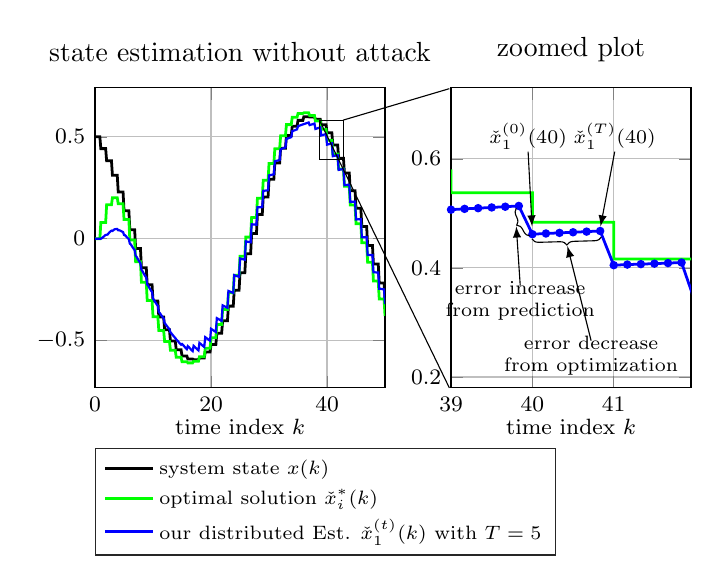
\begin{tikzpicture}
	\begin{axis}
	[	width=1.45in,
		height=1.5in,
		at={(0in,0in)},
		scale only axis,
		xmin=0,
		xmax=50.0,
		title=state estimation without attack,
		xlabel={\footnotesize time index $k$},
%		ylabel={\footnotesize value of state 2},
		x label style={at={(axis description cs:0.5,-0.07)},anchor=north},
		y label style={at={(axis description cs:0.1,.5)},anchor=south},
		xticklabel style = {font=\footnotesize},
		yticklabel style = {font=\footnotesize},
		axis background/.style={fill=white},
		xmajorgrids,
		ymajorgrids,
		legend style={at={(0,-0.2)}, anchor=north west, legend cell align=left, align=left, legend columns=1, draw=white!15!black, font=\scriptsize }]
		\addplot [color={black}, line width=1pt]
		table[row sep={\\}]
		{        0.0  0.5  \\
			0.16666666666666666  0.5  \\
			0.3333333333333333  0.5  \\
			0.5  0.5  \\
			0.6666666666666666  0.5  \\
			0.8333333333333334  0.5  \\
			1.0  0.442141680080005  \\
			1.1666666666666667  0.442141680080005  \\
			1.3333333333333333  0.442141680080005  \\
			1.5  0.442141680080005  \\
			1.6666666666666667  0.442141680080005  \\
			1.8333333333333333  0.442141680080005  \\
			2.0  0.38250853906313464  \\
			2.1666666666666665  0.38250853906313464  \\
			2.3333333333333335  0.38250853906313464  \\
			2.5  0.38250853906313464  \\
			2.6666666666666665  0.38250853906313464  \\
			2.8333333333333335  0.38250853906313464  \\
			3.0  0.311166640903765  \\
			3.1666666666666665  0.311166640903765  \\
			3.3333333333333335  0.311166640903765  \\
			3.5  0.311166640903765  \\
			3.6666666666666665  0.311166640903765  \\
			3.8333333333333335  0.311166640903765  \\
			4.0  0.2297777388395434  \\
			4.166666666666667  0.2297777388395434  \\
			4.333333333333333  0.2297777388395434  \\
			4.5  0.2297777388395434  \\
			4.666666666666667  0.2297777388395434  \\
			4.833333333333333  0.2297777388395434  \\
			5.0  0.13748929175546973  \\
			5.166666666666667  0.13748929175546973  \\
			5.333333333333333  0.13748929175546973  \\
			5.5  0.13748929175546973  \\
			5.666666666666667  0.13748929175546973  \\
			5.833333333333333  0.13748929175546973  \\
			6.0  0.044429088602335784  \\
			6.166666666666667  0.044429088602335784  \\
			6.333333333333333  0.044429088602335784  \\
			6.5  0.044429088602335784  \\
			6.666666666666667  0.044429088602335784  \\
			6.833333333333333  0.044429088602335784  \\
			7.0  -0.04792567851312916  \\
			7.166666666666667  -0.04792567851312916  \\
			7.333333333333333  -0.04792567851312916  \\
			7.5  -0.04792567851312916  \\
			7.666666666666667  -0.04792567851312916  \\
			7.833333333333333  -0.04792567851312916  \\
			8.0  -0.14177366138169356  \\
			8.166666666666666  -0.14177366138169356  \\
			8.333333333333334  -0.14177366138169356  \\
			8.5  -0.14177366138169356  \\
			8.666666666666666  -0.14177366138169356  \\
			8.833333333333334  -0.14177366138169356  \\
			9.0  -0.22615878403615564  \\
			9.166666666666666  -0.22615878403615564  \\
			9.333333333333334  -0.22615878403615564  \\
			9.5  -0.22615878403615564  \\
			9.666666666666666  -0.22615878403615564  \\
			9.833333333333334  -0.22615878403615564  \\
			10.0  -0.3056894389363811  \\
			10.166666666666666  -0.3056894389363811  \\
			10.333333333333334  -0.3056894389363811  \\
			10.5  -0.3056894389363811  \\
			10.666666666666666  -0.3056894389363811  \\
			10.833333333333334  -0.3056894389363811  \\
			11.0  -0.3840453224536651  \\
			11.166666666666666  -0.3840453224536651  \\
			11.333333333333334  -0.3840453224536651  \\
			11.5  -0.3840453224536651  \\
			11.666666666666666  -0.3840453224536651  \\
			11.833333333333334  -0.3840453224536651  \\
			12.0  -0.44656955439326446  \\
			12.166666666666666  -0.44656955439326446  \\
			12.333333333333334  -0.44656955439326446  \\
			12.5  -0.44656955439326446  \\
			12.666666666666666  -0.44656955439326446  \\
			12.833333333333334  -0.44656955439326446  \\
			13.0  -0.5013259383143396  \\
			13.166666666666666  -0.5013259383143396  \\
			13.333333333333334  -0.5013259383143396  \\
			13.5  -0.5013259383143396  \\
			13.666666666666666  -0.5013259383143396  \\
			13.833333333333334  -0.5013259383143396  \\
			14.0  -0.5440571584478838  \\
			14.166666666666666  -0.5440571584478838  \\
			14.333333333333334  -0.5440571584478838  \\
			14.5  -0.5440571584478838  \\
			14.666666666666666  -0.5440571584478838  \\
			14.833333333333334  -0.5440571584478838  \\
			15.0  -0.5752095614567391  \\
			15.166666666666666  -0.5752095614567391  \\
			15.333333333333334  -0.5752095614567391  \\
			15.5  -0.5752095614567391  \\
			15.666666666666666  -0.5752095614567391  \\
			15.833333333333334  -0.5752095614567391  \\
			16.0  -0.5895300541609215  \\
			16.166666666666668  -0.5895300541609215  \\
			16.333333333333332  -0.5895300541609215  \\
			16.5  -0.5895300541609215  \\
			16.666666666666668  -0.5895300541609215  \\
			16.833333333333332  -0.5895300541609215  \\
			17.0  -0.5937076218792638  \\
			17.166666666666668  -0.5937076218792638  \\
			17.333333333333332  -0.5937076218792638  \\
			17.5  -0.5937076218792638  \\
			17.666666666666668  -0.5937076218792638  \\
			17.833333333333332  -0.5937076218792638  \\
			18.0  -0.5851706798426926  \\
			18.166666666666668  -0.5851706798426926  \\
			18.333333333333332  -0.5851706798426926  \\
			18.5  -0.5851706798426926  \\
			18.666666666666668  -0.5851706798426926  \\
			18.833333333333332  -0.5851706798426926  \\
			19.0  -0.5553247766084655  \\
			19.166666666666668  -0.5553247766084655  \\
			19.333333333333332  -0.5553247766084655  \\
			19.5  -0.5553247766084655  \\
			19.666666666666668  -0.5553247766084655  \\
			19.833333333333332  -0.5553247766084655  \\
			20.0  -0.5190321506605758  \\
			20.166666666666668  -0.5190321506605758  \\
			20.333333333333332  -0.5190321506605758  \\
			20.5  -0.5190321506605758  \\
			20.666666666666668  -0.5190321506605758  \\
			20.833333333333332  -0.5190321506605758  \\
			21.0  -0.46392210934025324  \\
			21.166666666666668  -0.46392210934025324  \\
			21.333333333333332  -0.46392210934025324  \\
			21.5  -0.46392210934025324  \\
			21.666666666666668  -0.46392210934025324  \\
			21.833333333333332  -0.46392210934025324  \\
			22.0  -0.402502309085297  \\
			22.166666666666668  -0.402502309085297  \\
			22.333333333333332  -0.402502309085297  \\
			22.5  -0.402502309085297  \\
			22.666666666666668  -0.402502309085297  \\
			22.833333333333332  -0.402502309085297  \\
			23.0  -0.3306169543223272  \\
			23.166666666666668  -0.3306169543223272  \\
			23.333333333333332  -0.3306169543223272  \\
			23.5  -0.3306169543223272  \\
			23.666666666666668  -0.3306169543223272  \\
			23.833333333333332  -0.3306169543223272  \\
			24.0  -0.253041795550178  \\
			24.166666666666668  -0.253041795550178  \\
			24.333333333333332  -0.253041795550178  \\
			24.5  -0.253041795550178  \\
			24.666666666666668  -0.253041795550178  \\
			24.833333333333332  -0.253041795550178  \\
			25.0  -0.16664600146683925  \\
			25.166666666666668  -0.16664600146683925  \\
			25.333333333333332  -0.16664600146683925  \\
			25.5  -0.16664600146683925  \\
			25.666666666666668  -0.16664600146683925  \\
			25.833333333333332  -0.16664600146683925  \\
			26.0  -0.07330586462801282  \\
			26.166666666666668  -0.07330586462801282  \\
			26.333333333333332  -0.07330586462801282  \\
			26.5  -0.07330586462801282  \\
			26.666666666666668  -0.07330586462801282  \\
			26.833333333333332  -0.07330586462801282  \\
			27.0  0.025266902403808033  \\
			27.166666666666668  0.025266902403808033  \\
			27.333333333333332  0.025266902403808033  \\
			27.5  0.025266902403808033  \\
			27.666666666666668  0.025266902403808033  \\
			27.833333333333332  0.025266902403808033  \\
			28.0  0.11928722612065801  \\
			28.166666666666668  0.11928722612065801  \\
			28.333333333333332  0.11928722612065801  \\
			28.5  0.11928722612065801  \\
			28.666666666666668  0.11928722612065801  \\
			28.833333333333332  0.11928722612065801  \\
			29.0  0.205022380105992  \\
			29.166666666666668  0.205022380105992  \\
			29.333333333333332  0.205022380105992  \\
			29.5  0.205022380105992  \\
			29.666666666666668  0.205022380105992  \\
			29.833333333333332  0.205022380105992  \\
			30.0  0.29215484951389864  \\
			30.166666666666668  0.29215484951389864  \\
			30.333333333333332  0.29215484951389864  \\
			30.5  0.29215484951389864  \\
			30.666666666666668  0.29215484951389864  \\
			30.833333333333332  0.29215484951389864  \\
			31.0  0.3718224720291013  \\
			31.166666666666668  0.3718224720291013  \\
			31.333333333333332  0.3718224720291013  \\
			31.5  0.3718224720291013  \\
			31.666666666666668  0.3718224720291013  \\
			31.833333333333332  0.3718224720291013  \\
			32.0  0.44407427456509946  \\
			32.166666666666664  0.44407427456509946  \\
			32.333333333333336  0.44407427456509946  \\
			32.5  0.44407427456509946  \\
			32.666666666666664  0.44407427456509946  \\
			32.833333333333336  0.44407427456509946  \\
			33.0  0.5065773980220284  \\
			33.166666666666664  0.5065773980220284  \\
			33.333333333333336  0.5065773980220284  \\
			33.5  0.5065773980220284  \\
			33.666666666666664  0.5065773980220284  \\
			33.833333333333336  0.5065773980220284  \\
			34.0  0.5514611014864197  \\
			34.166666666666664  0.5514611014864197  \\
			34.333333333333336  0.5514611014864197  \\
			34.5  0.5514611014864197  \\
			34.666666666666664  0.5514611014864197  \\
			34.833333333333336  0.5514611014864197  \\
			35.0  0.5807150363798887  \\
			35.166666666666664  0.5807150363798887  \\
			35.333333333333336  0.5807150363798887  \\
			35.5  0.5807150363798887  \\
			35.666666666666664  0.5807150363798887  \\
			35.833333333333336  0.5807150363798887  \\
			36.0  0.5982969753075194  \\
			36.166666666666664  0.5982969753075194  \\
			36.333333333333336  0.5982969753075194  \\
			36.5  0.5982969753075194  \\
			36.666666666666664  0.5982969753075194  \\
			36.833333333333336  0.5982969753075194  \\
			37.0  0.5967371746283066  \\
			37.166666666666664  0.5967371746283066  \\
			37.333333333333336  0.5967371746283066  \\
			37.5  0.5967371746283066  \\
			37.666666666666664  0.5967371746283066  \\
			37.833333333333336  0.5967371746283066  \\
			38.0  0.5861688192665043  \\
			38.166666666666664  0.5861688192665043  \\
			38.333333333333336  0.5861688192665043  \\
			38.5  0.5861688192665043  \\
			38.666666666666664  0.5861688192665043  \\
			38.833333333333336  0.5861688192665043  \\
			39.0  0.55916233987193  \\
			39.166666666666664  0.55916233987193  \\
			39.333333333333336  0.55916233987193  \\
			39.5  0.55916233987193  \\
			39.666666666666664  0.55916233987193  \\
			39.833333333333336  0.55916233987193  \\
			40.0  0.519713080932801  \\
			40.166666666666664  0.519713080932801  \\
			40.333333333333336  0.519713080932801  \\
			40.5  0.519713080932801  \\
			40.666666666666664  0.519713080932801  \\
			40.833333333333336  0.519713080932801  \\
			41.0  0.4600516271366207  \\
			41.166666666666664  0.4600516271366207  \\
			41.333333333333336  0.4600516271366207  \\
			41.5  0.4600516271366207  \\
			41.666666666666664  0.4600516271366207  \\
			41.833333333333336  0.4600516271366207  \\
			42.0  0.3951064216465147  \\
			42.166666666666664  0.3951064216465147  \\
			42.333333333333336  0.3951064216465147  \\
			42.5  0.3951064216465147  \\
			42.666666666666664  0.3951064216465147  \\
			42.833333333333336  0.3951064216465147  \\
			43.0  0.32243155646908406  \\
			43.166666666666664  0.32243155646908406  \\
			43.333333333333336  0.32243155646908406  \\
			43.5  0.32243155646908406  \\
			43.666666666666664  0.32243155646908406  \\
			43.833333333333336  0.32243155646908406  \\
			44.0  0.23569401641650506  \\
			44.166666666666664  0.23569401641650506  \\
			44.333333333333336  0.23569401641650506  \\
			44.5  0.23569401641650506  \\
			44.666666666666664  0.23569401641650506  \\
			44.833333333333336  0.23569401641650506  \\
			45.0  0.1494177688804219  \\
			45.166666666666664  0.1494177688804219  \\
			45.333333333333336  0.1494177688804219  \\
			45.5  0.1494177688804219  \\
			45.666666666666664  0.1494177688804219  \\
			45.833333333333336  0.1494177688804219  \\
			46.0  0.06030012470653266  \\
			46.166666666666664  0.06030012470653266  \\
			46.333333333333336  0.06030012470653266  \\
			46.5  0.06030012470653266  \\
			46.666666666666664  0.06030012470653266  \\
			46.833333333333336  0.06030012470653266  \\
			47.0  -0.03357916412344015  \\
			47.166666666666664  -0.03357916412344015  \\
			47.333333333333336  -0.03357916412344015  \\
			47.5  -0.03357916412344015  \\
			47.666666666666664  -0.03357916412344015  \\
			47.833333333333336  -0.03357916412344015  \\
			48.0  -0.12394962941961828  \\
			48.166666666666664  -0.12394962941961828  \\
			48.333333333333336  -0.12394962941961828  \\
			48.5  -0.12394962941961828  \\
			48.666666666666664  -0.12394962941961828  \\
			48.833333333333336  -0.12394962941961828  \\
			49.0  -0.2173640219125626  \\
			49.166666666666664  -0.2173640219125626  \\
			49.333333333333336  -0.2173640219125626  \\
			49.5  -0.2173640219125626  \\
			49.666666666666664  -0.2173640219125626  \\
			49.833333333333336  -0.2173640219125626  \\
			50.0  -0.3049548419970705  \\
		}
		;\addlegendentry{system state $x(k)$}
		
		
		\addplot [color={green}, line width=1pt]
		table[row sep={\\}]
		{
		       0.0  0.0  \\
		      0.16666666666666666  0.0  \\
		      0.3333333333333333  0.0  \\
		      0.5  0.0  \\
		      0.6666666666666666  0.0  \\
		      0.8333333333333334  0.0  \\
		      1.0  0.07915473069094893  \\
		      1.1666666666666667  0.07915473069094893  \\
		      1.3333333333333333  0.07915473069094893  \\
		      1.5  0.07915473069094893  \\
		      1.6666666666666667  0.07915473069094893  \\
		      1.8333333333333333  0.07915473069094893  \\
		      2.0  0.16648622036352356  \\
		      2.1666666666666665  0.16648622036352356  \\
		      2.3333333333333335  0.16648622036352356  \\
		      2.5  0.16648622036352356  \\
		      2.6666666666666665  0.16648622036352356  \\
		      2.8333333333333335  0.16648622036352356  \\
		      3.0  0.20057434449488282  \\
		      3.1666666666666665  0.20057434449488282  \\
		      3.3333333333333335  0.20057434449488282  \\
		      3.5  0.20057434449488282  \\
		      3.6666666666666665  0.20057434449488282  \\
		      3.8333333333333335  0.20057434449488282  \\
		      4.0  0.17155519638348105  \\
		      4.166666666666667  0.17155519638348105  \\
		      4.333333333333333  0.17155519638348105  \\
		      4.5  0.17155519638348105  \\
		      4.666666666666667  0.17155519638348105  \\
		      4.833333333333333  0.17155519638348105  \\
		      5.0  0.09431376066971828  \\
		      5.166666666666667  0.09431376066971828  \\
		      5.333333333333333  0.09431376066971828  \\
		      5.5  0.09431376066971828  \\
		      5.666666666666667  0.09431376066971828  \\
		      5.833333333333333  0.09431376066971828  \\
		      6.0  -0.006438053737108274  \\
		      6.166666666666667  -0.006438053737108274  \\
		      6.333333333333333  -0.006438053737108274  \\
		      6.5  -0.006438053737108274  \\
		      6.666666666666667  -0.006438053737108274  \\
		      6.833333333333333  -0.006438053737108274  \\
		      7.0  -0.11264552863004094  \\
		      7.166666666666667  -0.11264552863004094  \\
		      7.333333333333333  -0.11264552863004094  \\
		      7.5  -0.11264552863004094  \\
		      7.666666666666667  -0.11264552863004094  \\
		      7.833333333333333  -0.11264552863004094  \\
		      8.0  -0.21345977163273352  \\
		      8.166666666666666  -0.21345977163273352  \\
		      8.333333333333334  -0.21345977163273352  \\
		      8.5  -0.21345977163273352  \\
		      8.666666666666666  -0.21345977163273352  \\
		      8.833333333333334  -0.21345977163273352  \\
		      9.0  -0.3029100762710078  \\
		      9.166666666666666  -0.3029100762710078  \\
		      9.333333333333334  -0.3029100762710078  \\
		      9.5  -0.3029100762710078  \\
		      9.666666666666666  -0.3029100762710078  \\
		      9.833333333333334  -0.3029100762710078  \\
		      10.0  -0.3823045110988261  \\
		      10.166666666666666  -0.3823045110988261  \\
		      10.333333333333334  -0.3823045110988261  \\
		      10.5  -0.3823045110988261  \\
		      10.666666666666666  -0.3823045110988261  \\
		      10.833333333333334  -0.3823045110988261  \\
		      11.0  -0.45026562103422063  \\
		      11.166666666666666  -0.45026562103422063  \\
		      11.333333333333334  -0.45026562103422063  \\
		      11.5  -0.45026562103422063  \\
		      11.666666666666666  -0.45026562103422063  \\
		      11.833333333333334  -0.45026562103422063  \\
		      12.0  -0.5042501037516995  \\
		      12.166666666666666  -0.5042501037516995  \\
		      12.333333333333334  -0.5042501037516995  \\
		      12.5  -0.5042501037516995  \\
		      12.666666666666666  -0.5042501037516995  \\
		      12.833333333333334  -0.5042501037516995  \\
		      13.0  -0.5475705522620906  \\
		      13.166666666666666  -0.5475705522620906  \\
		      13.333333333333334  -0.5475705522620906  \\
		      13.5  -0.5475705522620906  \\
		      13.666666666666666  -0.5475705522620906  \\
		      13.833333333333334  -0.5475705522620906  \\
		      14.0  -0.581638912698449  \\
		      14.166666666666666  -0.581638912698449  \\
		      14.333333333333334  -0.581638912698449  \\
		      14.5  -0.581638912698449  \\
		      14.666666666666666  -0.581638912698449  \\
		      14.833333333333334  -0.581638912698449  \\
		      15.0  -0.6037299693374732  \\
		      15.166666666666666  -0.6037299693374732  \\
		      15.333333333333334  -0.6037299693374732  \\
		      15.5  -0.6037299693374732  \\
		      15.666666666666666  -0.6037299693374732  \\
		      15.833333333333334  -0.6037299693374732  \\
		      16.0  -0.60899207192653  \\
		      16.166666666666668  -0.60899207192653  \\
		      16.333333333333332  -0.60899207192653  \\
		      16.5  -0.60899207192653  \\
		      16.666666666666668  -0.60899207192653  \\
		      16.833333333333332  -0.60899207192653  \\
		      17.0  -0.6010024007839774  \\
		      17.166666666666668  -0.6010024007839774  \\
		      17.333333333333332  -0.6010024007839774  \\
		      17.5  -0.6010024007839774  \\
		      17.666666666666668  -0.6010024007839774  \\
		      17.833333333333332  -0.6010024007839774  \\
		      18.0  -0.5787423502141331  \\
		      18.166666666666668  -0.5787423502141331  \\
		      18.333333333333332  -0.5787423502141331  \\
		      18.5  -0.5787423502141331  \\
		      18.666666666666668  -0.5787423502141331  \\
		      18.833333333333332  -0.5787423502141331  \\
		      19.0  -0.5375229297893186  \\
		      19.166666666666668  -0.5375229297893186  \\
		      19.333333333333332  -0.5375229297893186  \\
		      19.5  -0.5375229297893186  \\
		      19.666666666666668  -0.5375229297893186  \\
		      19.833333333333332  -0.5375229297893186  \\
		      20.0  -0.4858767554676809  \\
		      20.166666666666668  -0.4858767554676809  \\
		      20.333333333333332  -0.4858767554676809  \\
		      20.5  -0.4858767554676809  \\
		      20.666666666666668  -0.4858767554676809  \\
		      20.833333333333332  -0.4858767554676809  \\
		      21.0  -0.42019141427642587  \\
		      21.166666666666668  -0.42019141427642587  \\
		      21.333333333333332  -0.42019141427642587  \\
		      21.5  -0.42019141427642587  \\
		      21.666666666666668  -0.42019141427642587  \\
		      21.833333333333332  -0.42019141427642587  \\
		      22.0  -0.34678225736589025  \\
		      22.166666666666668  -0.34678225736589025  \\
		      22.333333333333332  -0.34678225736589025  \\
		      22.5  -0.34678225736589025  \\
		      22.666666666666668  -0.34678225736589025  \\
		      22.833333333333332  -0.34678225736589025  \\
		      23.0  -0.26535238289309165  \\
		      23.166666666666668  -0.26535238289309165  \\
		      23.333333333333332  -0.26535238289309165  \\
		      23.5  -0.26535238289309165  \\
		      23.666666666666668  -0.26535238289309165  \\
		      23.833333333333332  -0.26535238289309165  \\
		      24.0  -0.17900836025251807  \\
		      24.166666666666668  -0.17900836025251807  \\
		      24.333333333333332  -0.17900836025251807  \\
		      24.5  -0.17900836025251807  \\
		      24.666666666666668  -0.17900836025251807  \\
		      24.833333333333332  -0.17900836025251807  \\
		      25.0  -0.0856090357304137  \\
		      25.166666666666668  -0.0856090357304137  \\
		      25.333333333333332  -0.0856090357304137  \\
		      25.5  -0.0856090357304137  \\
		      25.666666666666668  -0.0856090357304137  \\
		      25.833333333333332  -0.0856090357304137  \\
		      26.0  0.008549022942407686  \\
		      26.166666666666668  0.008549022942407686  \\
		      26.333333333333332  0.008549022942407686  \\
		      26.5  0.008549022942407686  \\
		      26.666666666666668  0.008549022942407686  \\
		      26.833333333333332  0.008549022942407686  \\
		      27.0  0.10383015984877979  \\
		      27.166666666666668  0.10383015984877979  \\
		      27.333333333333332  0.10383015984877979  \\
		      27.5  0.10383015984877979  \\
		      27.666666666666668  0.10383015984877979  \\
		      27.833333333333332  0.10383015984877979  \\
		      28.0  0.1982365034635945  \\
		      28.166666666666668  0.1982365034635945  \\
		      28.333333333333332  0.1982365034635945  \\
		      28.5  0.1982365034635945  \\
		      28.666666666666668  0.1982365034635945  \\
		      28.833333333333332  0.1982365034635945  \\
		      29.0  0.28642239223330396  \\
		      29.166666666666668  0.28642239223330396  \\
		      29.333333333333332  0.28642239223330396  \\
		      29.5  0.28642239223330396  \\
		      29.666666666666668  0.28642239223330396  \\
		      29.833333333333332  0.28642239223330396  \\
		      30.0  0.36900666812723776  \\
		      30.166666666666668  0.36900666812723776  \\
		      30.333333333333332  0.36900666812723776  \\
		      30.5  0.36900666812723776  \\
		      30.666666666666668  0.36900666812723776  \\
		      30.833333333333332  0.36900666812723776  \\
		      31.0  0.44131765589785515  \\
		      31.166666666666668  0.44131765589785515  \\
		      31.333333333333332  0.44131765589785515  \\
		      31.5  0.44131765589785515  \\
		      31.666666666666668  0.44131765589785515  \\
		      31.833333333333332  0.44131765589785515  \\
		      32.0  0.5056474775326305  \\
		      32.166666666666664  0.5056474775326305  \\
		      32.333333333333336  0.5056474775326305  \\
		      32.5  0.5056474775326305  \\
		      32.666666666666664  0.5056474775326305  \\
		      32.833333333333336  0.5056474775326305  \\
		      33.0  0.5598282599635899  \\
		      33.166666666666664  0.5598282599635899  \\
		      33.333333333333336  0.5598282599635899  \\
		      33.5  0.5598282599635899  \\
		      33.666666666666664  0.5598282599635899  \\
		      33.833333333333336  0.5598282599635899  \\
		      34.0  0.5958279649780339  \\
		      34.166666666666664  0.5958279649780339  \\
		      34.333333333333336  0.5958279649780339  \\
		      34.5  0.5958279649780339  \\
		      34.666666666666664  0.5958279649780339  \\
		      34.833333333333336  0.5958279649780339  \\
		      35.0  0.6149418952860649  \\
		      35.166666666666664  0.6149418952860649  \\
		      35.333333333333336  0.6149418952860649  \\
		      35.5  0.6149418952860649  \\
		      35.666666666666664  0.6149418952860649  \\
		      35.833333333333336  0.6149418952860649  \\
		      36.0  0.6175944190099131  \\
		      36.166666666666664  0.6175944190099131  \\
		      36.333333333333336  0.6175944190099131  \\
		      36.5  0.6175944190099131  \\
		      36.666666666666664  0.6175944190099131  \\
		      36.833333333333336  0.6175944190099131  \\
		      37.0  0.6045431714431487  \\
		      37.166666666666664  0.6045431714431487  \\
		      37.333333333333336  0.6045431714431487  \\
		      37.5  0.6045431714431487  \\
		      37.666666666666664  0.6045431714431487  \\
		      37.833333333333336  0.6045431714431487  \\
		      38.0  0.5781619633875313  \\
		      38.166666666666664  0.5781619633875313  \\
		      38.333333333333336  0.5781619633875313  \\
		      38.5  0.5781619633875313  \\
		      38.666666666666664  0.5781619633875313  \\
		      38.833333333333336  0.5781619633875313  \\
		      39.0  0.5376779646409742  \\
		      39.166666666666664  0.5376779646409742  \\
		      39.333333333333336  0.5376779646409742  \\
		      39.5  0.5376779646409742  \\
		      39.666666666666664  0.5376779646409742  \\
		      39.833333333333336  0.5376779646409742  \\
		      40.0  0.48363191995146726  \\
		      40.166666666666664  0.48363191995146726  \\
		      40.333333333333336  0.48363191995146726  \\
		      40.5  0.48363191995146726  \\
		      40.666666666666664  0.48363191995146726  \\
		      40.833333333333336  0.48363191995146726  \\
		      41.0  0.41607150447511027  \\
		      41.166666666666664  0.41607150447511027  \\
		      41.333333333333336  0.41607150447511027  \\
		      41.5  0.41607150447511027  \\
		      41.666666666666664  0.41607150447511027  \\
		      41.833333333333336  0.41607150447511027  \\
		      42.0  0.341726598171413  \\
		      42.166666666666664  0.341726598171413  \\
		      42.333333333333336  0.341726598171413  \\
		      42.5  0.341726598171413  \\
		      42.666666666666664  0.341726598171413  \\
		      42.833333333333336  0.341726598171413  \\
		      43.0  0.25758750045774587  \\
		      43.166666666666664  0.25758750045774587  \\
		      43.333333333333336  0.25758750045774587  \\
		      43.5  0.25758750045774587  \\
		      43.666666666666664  0.25758750045774587  \\
		      43.833333333333336  0.25758750045774587  \\
		      44.0  0.1660578234813623  \\
		      44.166666666666664  0.1660578234813623  \\
		      44.333333333333336  0.1660578234813623  \\
		      44.5  0.1660578234813623  \\
		      44.666666666666664  0.1660578234813623  \\
		      44.833333333333336  0.1660578234813623  \\
		      45.0  0.07314398633273098  \\
		      45.166666666666664  0.07314398633273098  \\
		      45.333333333333336  0.07314398633273098  \\
		      45.5  0.07314398633273098  \\
		      45.666666666666664  0.07314398633273098  \\
		      45.833333333333336  0.07314398633273098  \\
		      46.0  -0.019949490386536383  \\
		      46.166666666666664  -0.019949490386536383  \\
		      46.333333333333336  -0.019949490386536383  \\
		      46.5  -0.019949490386536383  \\
		      46.666666666666664  -0.019949490386536383  \\
		      46.833333333333336  -0.019949490386536383  \\
		      47.0  -0.11504125314316961  \\
		      47.166666666666664  -0.11504125314316961  \\
		      47.333333333333336  -0.11504125314316961  \\
		      47.5  -0.11504125314316961  \\
		      47.666666666666664  -0.11504125314316961  \\
		      47.833333333333336  -0.11504125314316961  \\
		      48.0  -0.20680638692126752  \\
		      48.166666666666664  -0.20680638692126752  \\
		      48.333333333333336  -0.20680638692126752  \\
		      48.5  -0.20680638692126752  \\
		      48.666666666666664  -0.20680638692126752  \\
		      48.833333333333336  -0.20680638692126752  \\
		      49.0  -0.29509128838149407  \\
		      49.166666666666664  -0.29509128838149407  \\
		      49.333333333333336  -0.29509128838149407  \\
		      49.5  -0.29509128838149407  \\
		      49.666666666666664  -0.29509128838149407  \\
		      49.833333333333336  -0.29509128838149407  \\
		      50.0  -0.37871921026452204  \\
		}
		;\addlegendentry{{optimal solution $\check{x}_i^*(k)$}}
		
%		\addplot[densely dotted, color={blue}, line width=1pt]
%		table[row sep={\\}]
%		{
%		   0.0  0.0  \\
%		 0.3333333333333333  0.0  \\
%		 0.6666666666666666  0.0  \\
%		 1.0  0.0  \\
%		 1.3333333333333333  -0.00712863348616053  \\
%		 1.6666666666666667  -0.01408036995322394  \\
%		 2.0  -0.015983938350976182  \\
%		 2.3333333333333335  -0.025307994519959152  \\
%		 2.6666666666666665  -0.03556603851550393  \\
%		 3.0  -0.03836804708425673  \\
%		 3.3333333333333335  -0.04865526044894676  \\
%		 3.6666666666666665  -0.060434189256829446  \\
%		 4.0  -0.06251971948554397  \\
%		 4.333333333333333  -0.07332251313985139  \\
%		 4.666666666666667  -0.08539388712765801  \\
%		 5.0  -0.0855024693156498  \\
%		 5.333333333333333  -0.09624117777401178  \\
%		 5.666666666666667  -0.10754196774083707  \\
%		 6.0  -0.10494634584281394  \\
%		 6.333333333333333  -0.11487412719369862  \\
%		 6.666666666666667  -0.12463324352154782  \\
%		 7.0  -0.11902245580585623  \\
%		 7.333333333333333  -0.12747098558413103  \\
%		 7.666666666666667  -0.13523436814062445  \\
%		 8.0  -0.12649486764707718  \\
%		 8.333333333333334  -0.13295811969318724  \\
%		 8.666666666666666  -0.1384954666368934  \\
%		 9.0  -0.1265405966097138  \\
%		 9.333333333333334  -0.13061030345120866  \\
%		 9.666666666666666  -0.13378356903068106  \\
%		 10.0  -0.1184709756811573  \\
%		 10.333333333333334  -0.12028565287023359  \\
%		 10.666666666666666  -0.12137157610892481  \\
%		 11.0  -0.10264285280662999  \\
%		 11.333333333333334  -0.10242742186556775  \\
%		 11.666666666666666  -0.10170709044538426  \\
%		 12.0  -0.07959466515002803  \\
%		 12.333333333333334  -0.07764597404614791  \\
%		 12.666666666666666  -0.07542658871467921  \\
%		 13.0  -0.05011300554670915  \\
%		 13.333333333333334  -0.047037400642047526  \\
%		 13.666666666666666  -0.04376622406947267  \\
%		 14.0  -0.015706304473777546  \\
%		 14.333333333333334  -0.011602961909547755  \\
%		 14.666666666666666  -0.0073934280234282295  \\
%		 15.0  0.022798103040236842  \\
%		 15.333333333333334  0.027781463180048246  \\
%		 15.666666666666666  0.03279840944534272  \\
%		 16.0  0.06434082267014991  \\
%		 16.333333333333332  0.06992579188853912  \\
%		 16.666666666666668  0.07550866239468257  \\
%		 17.0  0.10743092480515826  \\
%		 17.333333333333332  0.11311358216986381  \\
%		 17.666666666666668  0.11887290129460848  \\
%		 18.0  0.14999100411466493  \\
%		 18.333333333333332  0.15590012083750932  \\
%		 18.666666666666668  0.16187140282666393  \\
%		 19.0  0.191039467261814  \\
%		 19.333333333333332  0.19697992491301244  \\
%		 19.666666666666668  0.20295936646442686  \\
%		 20.0  0.2290160419222466  \\
%		 20.333333333333332  0.23488092429955232  \\
%		 20.666666666666668  0.24072797144670938  \\
%		 21.0  0.2625751577427306  \\
%		 21.333333333333332  0.26795147781529727  \\
%		 21.666666666666668  0.27336849375125966  \\
%		 22.0  0.28993381676036395  \\
%		 22.333333333333332  0.2949954081679703  \\
%		 22.666666666666668  0.3000704621021787  \\
%		 23.0  0.31049787202137846  \\
%		 23.333333333333332  0.31528639055037533  \\
%		 23.666666666666668  0.3200019014839581  \\
%		 24.0  0.32363714407758043  \\
%		 24.333333333333332  0.3277687611822981  \\
%		 24.666666666666668  0.3318481236056613  \\
%		 25.0  0.32814765198818746  \\
%		 25.333333333333332  0.3318035550479369  \\
%		 25.666666666666668  0.335356965115145  \\
%		 26.0  0.32406480427599166  \\
%		 26.333333333333332  0.3269589012004645  \\
%		 26.666666666666668  0.32976846653889974  \\
%		 27.0  0.31077693011696866  \\
%		 27.333333333333332  0.31309479914673893  \\
%		 27.666666666666668  0.31524576522307124  \\
%		 28.0  0.28875559526582684  \\
%		 28.333333333333332  0.29015727460108165  \\
%		 28.666666666666668  0.2913972959489508  \\
%		 29.0  0.2577684556656997  \\
%		 29.333333333333332  0.2583240173770789  \\
%		 29.666666666666668  0.25869806258980776  \\
%		 30.0  0.21856561995286466  \\
%		 30.333333333333332  0.21836112069083063  \\
%		 30.666666666666668  0.21796800117202733  \\
%		 31.0  0.17222670684661853  \\
%		 31.333333333333332  0.17140922584635382  \\
%		 31.666666666666668  0.17039908667305054  \\
%		 32.0  0.12015893336307279  \\
%		 32.333333333333336  0.11886520624991262  \\
%		 32.666666666666664  0.11733415635891177  \\
%		 33.0  0.06387185730845349  \\
%		 33.333333333333336  0.06185532842635079  \\
%		 33.666666666666664  0.05966620594696724  \\
%		 34.0  0.0042933197694844175  \\
%		 34.333333333333336  0.0019079940493141661  \\
%		 34.666666666666664  -0.0006618921731566733  \\
%		 35.0  -0.05645817773757346  \\
%		 35.333333333333336  -0.05933005827839971  \\
%		 35.666666666666664  -0.062334760807147185  \\
%		 36.0  -0.11708214490620289  \\
%		 36.333333333333336  -0.12029411287562577  \\
%		 36.666666666666664  -0.1235843206393898  \\
%		 37.0  -0.17577975897570175  \\
%		 37.333333333333336  -0.17904642423098757  \\
%		 37.666666666666664  -0.18240584924590067  \\
%		 38.0  -0.23053251295207605  \\
%		 38.333333333333336  -0.23407449142794515  \\
%		 38.666666666666664  -0.23762051309104926  \\
%		 39.0  -0.28034060119157667  \\
%		 39.333333333333336  -0.2838036636991814  \\
%		 39.666666666666664  -0.2872886198212402  \\
%		 40.0  -0.3233055409741396  \\
%		 40.333333333333336  -0.32659337756116874  \\
%		 40.666666666666664  -0.3299182045343599  \\
%		 41.0  -0.35808367153751264  \\
%		 41.333333333333336  -0.36130450991107727  \\
%		 41.666666666666664  -0.3645061447321196  \\
%		 42.0  -0.383923231032246  \\
%		 42.333333333333336  -0.3869415552835787  \\
%		 42.666666666666664  -0.3899433989384339  \\
%		 43.0  -0.39991944945734315  \\
%		 43.333333333333336  -0.40274644115285885  \\
%		 43.666666666666664  -0.4055211149641161  \\
%		 44.0  -0.40560700709983066  \\
%		 44.333333333333336  -0.4082176041248438  \\
%		 44.666666666666664  -0.41072735458230664  \\
%		 45.0  -0.40074299558878845  \\
%		 45.333333333333336  -0.4028392394780222  \\
%		 45.666666666666664  -0.4048912580626767  \\
%		 46.0  -0.3848507208305408  \\
%		 46.333333333333336  -0.38673264569463134  \\
%		 46.666666666666664  -0.3885274648746461  \\
%		 47.0  -0.3588174907769079  \\
%		 47.333333333333336  -0.36037201330824453  \\
%		 47.666666666666664  -0.3618337616782129  \\
%		 48.0  -0.32306659393112835  \\
%		 48.333333333333336  -0.32430787336128797  \\
%		 48.666666666666664  -0.3254679767778187  \\
%		 49.0  -0.27850250853140873  \\
%		 49.333333333333336  -0.27960783315558385  \\
%		 49.666666666666664  -0.2805590563100507  \\
%		 50.0  -0.2265150430678405  \\
%	};\addlegendentry{$\check{x}_1^{(t)}(k)$ with $T=2$}

	\addplot[ color={blue}, line width=0.8pt]
table[row sep={\\}]
{
    0.0  0.0  \\
    0.16666666666666666  0.0  \\
    0.3333333333333333  0.0  \\
    0.5  0.0  \\
    0.6666666666666666  0.0  \\
    0.8333333333333334  0.0  \\
    1.0  0.0  \\
    1.1666666666666667  0.0028596726583446593  \\
    1.3333333333333333  0.0063541066448139834  \\
    1.5  0.010637467363894634  \\
    1.6666666666666667  0.014847207432920867  \\
    1.8333333333333333  0.018716718609563483  \\
    2.0  0.019446292136974925  \\
    2.1666666666666665  0.02045365233544711  \\
    2.3333333333333335  0.026407697371626376  \\
    2.5  0.031790181412424894  \\
    2.6666666666666665  0.03614035030249265  \\
    2.8333333333333335  0.039543098278167696  \\
    3.0  0.03818650837059714  \\
    3.1666666666666665  0.042016435348378595  \\
    3.3333333333333335  0.045588868088530375  \\
    3.5  0.047076054812111766  \\
    3.6666666666666665  0.04755922852123091  \\
    3.8333333333333335  0.04775126517022604  \\
    4.0  0.0413543285814679  \\
    4.166666666666667  0.041509982494437714  \\
    4.333333333333333  0.040088836207628674  \\
    4.5  0.03758281058189731  \\
    4.666666666666667  0.035025551818953976  \\
    4.833333333333333  0.03286676375299538  \\
    5.0  0.01894757621506936  \\
    5.166666666666667  0.01731138858541747  \\
    5.333333333333333  0.012418380419877157  \\
    5.5  0.007008465381465599  \\
    5.666666666666667  0.001990547256472199  \\
    5.833333333333333  -0.0023465553831833186  \\
    6.0  -0.023893165425746772  \\
    6.166666666666667  -0.02748720919427916  \\
    6.333333333333333  -0.03502638257405738  \\
    6.5  -0.04261255145165628  \\
    6.666666666666667  -0.04948227910682525  \\
    6.833333333333333  -0.05546830976885524  \\
    7.0  -0.08341025861315417  \\
    7.166666666666667  -0.08850240917452873  \\
    7.333333333333333  -0.0972616847194942  \\
    7.5  -0.10578256714479942  \\
    7.666666666666667  -0.11345470589399985  \\
    7.833333333333333  -0.12019867194053616  \\
    8.0  -0.15236002452229008  \\
    8.166666666666666  -0.15818643471545601  \\
    8.333333333333334  -0.1671972259932667  \\
    8.5  -0.17585669179878063  \\
    8.666666666666666  -0.18366676639296167  \\
    8.833333333333334  -0.1905843693289209  \\
    9.0  -0.22433317984488454  \\
    9.166666666666666  -0.23037786595509369  \\
    9.333333333333334  -0.23900126623365883  \\
    9.5  -0.24730565739823246  \\
    9.666666666666666  -0.25487530890425525  \\
    9.833333333333334  -0.2616685331065679  \\
    10.0  -0.29438301893767166  \\
    10.166666666666666  -0.300407751969211  \\
    10.333333333333334  -0.3084074905607778  \\
    10.5  -0.3160740865447425  \\
    10.666666666666666  -0.3231011140772536  \\
    10.833333333333334  -0.329456463992369  \\
    11.0  -0.3586065135943683  \\
    11.166666666666666  -0.3642710726618711  \\
    11.333333333333334  -0.37159522242894877  \\
    11.5  -0.37858616245011073  \\
    11.666666666666666  -0.3849967961027978  \\
    11.833333333333334  -0.39080763329343493  \\
    12.0  -0.4140863911051217  \\
    12.166666666666666  -0.4192922035631776  \\
    12.333333333333334  -0.42583719033524114  \\
    12.5  -0.4321689373289259  \\
    12.666666666666666  -0.43808081645349656  \\
    12.833333333333334  -0.4435329536209108  \\
    13.0  -0.4591180823869724  \\
    13.166666666666666  -0.46408137979731806  \\
    13.333333333333334  -0.47025321258580915  \\
    13.5  -0.4762386785994719  \\
    13.666666666666666  -0.481834716437993  \\
    13.833333333333334  -0.48699037008121565  \\
    14.0  -0.4935333588061507  \\
    14.166666666666666  -0.49821152790972445  \\
    14.333333333333334  -0.5040328585663597  \\
    14.5  -0.5097019585953517  \\
    14.666666666666666  -0.5150086292649508  \\
    14.833333333333334  -0.5199035786279858  \\
    15.0  -0.5163044239303488  \\
    15.166666666666666  -0.5207562928576478  \\
    15.333333333333334  -0.5263287640730334  \\
    15.5  -0.5318003401550352  \\
    15.666666666666666  -0.5369219440156179  \\
    15.833333333333334  -0.5416307064545095  \\
    16.0  -0.5271341597890151  \\
    16.166666666666668  -0.5314082560877575  \\
    16.333333333333332  -0.5365743844629505  \\
    16.5  -0.5417332122956809  \\
    16.666666666666668  -0.5466222621399857  \\
    16.833333333333332  -0.5511603524377469  \\
    17.0  -0.5254588634621442  \\
    17.166666666666668  -0.5296154159379026  \\
    17.333333333333332  -0.5343469205731622  \\
    17.5  -0.539090369282835  \\
    17.666666666666668  -0.5435984804723536  \\
    17.833333333333332  -0.5477870251864552  \\
    18.0  -0.5108376483094051  \\
    18.166666666666668  -0.5146558884453228  \\
    18.333333333333332  -0.5189048471804208  \\
    18.5  -0.523129930424258  \\
    18.666666666666668  -0.5271442373369738  \\
    18.833333333333332  -0.5308785119467823  \\
    19.0  -0.4828628477497462  \\
    19.166666666666668  -0.48626997033007624  \\
    19.333333333333332  -0.4898637638647399  \\
    19.5  -0.49348313016985296  \\
    19.666666666666668  -0.4969933617618095  \\
    19.833333333333332  -0.5003212268893816  \\
    20.0  -0.44191965422345475  \\
    20.166666666666668  -0.4450060416091525  \\
    20.333333333333332  -0.4482006854012597  \\
    20.5  -0.4513699463177552  \\
    20.666666666666668  -0.45443145453266554  \\
    20.833333333333332  -0.4573247735809402  \\
    21.0  -0.38955502775519824  \\
    21.166666666666668  -0.3922072945910434  \\
    21.333333333333332  -0.39488773653594356  \\
    21.5  -0.3976603824448868  \\
    21.666666666666668  -0.40037004857540165  \\
    21.833333333333332  -0.4029344794537435  \\
    22.0  -0.32710199959917385  \\
    22.166666666666668  -0.3294705515500897  \\
    22.333333333333332  -0.33174144668036926  \\
    22.5  -0.3340965308108121  \\
    22.666666666666668  -0.33640555474468176  \\
    22.833333333333332  -0.3385927682459531  \\
    23.0  -0.25633387999123936  \\
    23.166666666666668  -0.2583298920521858  \\
    23.333333333333332  -0.2601716915289446  \\
    23.5  -0.26205300398071707  \\
    23.666666666666668  -0.26391057806720963  \\
    23.833333333333332  -0.26568677606636804  \\
    24.0  -0.17868542338725557  \\
    24.166666666666668  -0.1803114845623962  \\
    24.333333333333332  -0.18188506844849406  \\
    24.5  -0.18353330011432353  \\
    24.666666666666668  -0.1851328893090518  \\
    24.833333333333332  -0.18662446017230463  \\
    25.0  -0.09681033754318635  \\
    25.166666666666668  -0.09815424169803223  \\
    25.333333333333332  -0.09931727770838053  \\
    25.5  -0.1005672846284372  \\
    25.666666666666668  -0.10184883432177673  \\
    25.833333333333332  -0.1031008680501307  \\
    26.0  -0.012658603889761089  \\
    26.166666666666668  -0.013812802664761684  \\
    26.333333333333332  -0.014701167859835761  \\
    26.5  -0.015661082003171144  \\
    26.666666666666668  -0.016640630618195512  \\
    26.833333333333332  -0.017582466266370184  \\
    27.0  0.07136774624151063  \\
    27.166666666666668  0.07053162665380294  \\
    27.333333333333332  0.07017869248358237  \\
    27.5  0.06973525202443649  \\
    27.666666666666668  0.06927321850839406  \\
    27.833333333333332  0.06883938787512948  \\
    28.0  0.15432287253210858  \\
    28.166666666666668  0.15396596546097718  \\
    28.333333333333332  0.15426848902997117  \\
    28.5  0.15457325842950456  \\
    28.666666666666668  0.1548145571080673  \\
    28.833333333333332  0.15500326935775618  \\
    29.0  0.23514039669598094  \\
    29.166666666666668  0.2353423805845928  \\
    29.333333333333332  0.2360042210269945  \\
    29.5  0.23667631581213425  \\
    29.666666666666668  0.23734260959123882  \\
    29.833333333333332  0.23800542569601327  \\
    30.0  0.31105594495363814  \\
    30.166666666666668  0.31173428431244077  \\
    30.333333333333332  0.31287236958708203  \\
    30.5  0.3140034250510714  \\
    30.666666666666668  0.3150566554255903  \\
    30.833333333333332  0.3160271188522871  \\
    31.0  0.38025435712058  \\
    31.166666666666668  0.3811721921396665  \\
    31.333333333333332  0.3824625448807691  \\
    31.5  0.38374101062563143  \\
    31.666666666666668  0.3849780886190861  \\
    31.833333333333332  0.3861657718002103  \\
    32.0  0.43998272046863773  \\
    32.166666666666664  0.4411310385691457  \\
    32.333333333333336  0.44282356198651873  \\
    32.5  0.44452924951280354  \\
    32.666666666666664  0.44613853683027055  \\
    32.833333333333336  0.44762837932041516  \\
    33.0  0.4896982159912828  \\
    33.166666666666664  0.49109402872930397  \\
    33.333333333333336  0.4929805474622135  \\
    33.5  0.4948945633913659  \\
    33.666666666666664  0.4967107769511928  \\
    33.833333333333336  0.498404287859952  \\
    34.0  0.5275959361766429  \\
    34.166666666666664  0.5291841304667074  \\
    34.333333333333336  0.5310656465063334  \\
    34.5  0.5329847400813219  \\
    34.666666666666664  0.5348657282665007  \\
    34.833333333333336  0.5366724536414897  \\
    35.0  0.5522056251317108  \\
    35.166666666666664  0.5539305070339705  \\
    35.333333333333336  0.5556621466606406  \\
    35.5  0.557406152359754  \\
    35.666666666666664  0.5591478093680529  \\
    35.833333333333336  0.5608591777013889  \\
    36.0  0.5622887890706182  \\
    36.166666666666664  0.5639381566512851  \\
    36.333333333333336  0.565525430821445  \\
    36.5  0.5671204070019282  \\
    36.666666666666664  0.5687212459192648  \\
    36.833333333333336  0.5702970944108869  \\
    37.0  0.5575183013510576  \\
    37.166666666666664  0.5590347755782731  \\
    37.333333333333336  0.5604965131803729  \\
    37.5  0.5620972883364147  \\
    37.666666666666664  0.5637188385480931  \\
    37.833333333333336  0.5652950319764657  \\
    38.0  0.5386545243297358  \\
    38.166666666666664  0.5401632694156049  \\
    38.333333333333336  0.5416277300524953  \\
    38.5  0.5432330504636081  \\
    38.666666666666664  0.5448574018318699  \\
    38.833333333333336  0.5464286609365481  \\
    39.0  0.5067166881815662  \\
    39.166666666666664  0.5081968972359134  \\
    39.333333333333336  0.5094600422726716  \\
    39.5  0.5107731096848483  \\
    39.666666666666664  0.5121471851969056  \\
    39.833333333333336  0.5135355672463893  \\
    40.0  0.46170669958052296  \\
    40.166666666666664  0.4630388972935881  \\
    40.333333333333336  0.4641500050054344  \\
    40.5  0.46528471305291463  \\
    40.666666666666664  0.46646391194835174  \\
    40.833333333333336  0.46764893165884297  \\
    41.0  0.4049199570470413  \\
    41.166666666666664  0.4060546535195703  \\
    41.333333333333336  0.4068715313825698  \\
    41.5  0.4077679553947931  \\
    41.666666666666664  0.40876142147601513  \\
    41.833333333333336  0.4098071625974  \\
    42.0  0.33782704394087154  \\
    42.166666666666664  0.3388589990385049  \\
    42.333333333333336  0.33959454908558756  \\
    42.5  0.3403926596613399  \\
    42.666666666666664  0.34122464709390493  \\
    42.833333333333336  0.34204414882446216  \\
    43.0  0.2625906180414062  \\
    43.166666666666664  0.2633388959116305  \\
    43.333333333333336  0.2637729048322996  \\
    43.5  0.2643111209584895  \\
    43.666666666666664  0.26489356220415533  \\
    43.833333333333336  0.265471576571562  \\
    44.0  0.18042933342188888  \\
    44.166666666666664  0.1809641891195692  \\
    44.333333333333336  0.18123344649574497  \\
    44.5  0.18167466204580834  \\
    44.666666666666664  0.18219966727397593  \\
    44.833333333333336  0.1827423921862862  \\
    45.0  0.09436890095205716  \\
    45.166666666666664  0.09488352979031381  \\
    45.333333333333336  0.09514590553331385  \\
    45.5  0.09554105643535293  \\
    45.666666666666664  0.09598586642511026  \\
    45.833333333333336  0.09642196608824337  \\
    46.0  0.007012880618347636  \\
    46.166666666666664  0.007389809945570034  \\
    46.333333333333336  0.0075086402871131774  \\
    46.5  0.007780696332186598  \\
    46.666666666666664  0.00809114848910706  \\
    46.833333333333336  0.008382631729170496  \\
    47.0  -0.07989028439950374  \\
    47.166666666666664  -0.07965395338091173  \\
    47.333333333333336  -0.07977497546772545  \\
    47.5  -0.0797829722974118  \\
    47.666666666666664  -0.07972438271942452  \\
    47.833333333333336  -0.07964839519260809  \\
    48.0  -0.16456390321304054  \\
    48.166666666666664  -0.164520697191884  \\
    48.333333333333336  -0.16491920957545847  \\
    48.5  -0.165266372905793  \\
    48.666666666666664  -0.1655635855818763  \\
    48.833333333333336  -0.16583595684366947  \\
    49.0  -0.245384488030023  \\
    49.166666666666664  -0.24567617836737993  \\
    49.333333333333336  -0.24642459633108008  \\
    49.5  -0.24715466340579426  \\
    49.666666666666664  -0.24781924545892892  \\
    49.833333333333336  -0.2484290616126222  \\
    50.0  -0.32069796979840737  \\
};\addlegendentry{ our distributed Est. $\check{x}_1^{(t)}(k)$ with $T=5$}
		
%		\addplot[ color={blue}, line width=1pt]
%		table[row sep={\\}]
%		{
%	        0.0  0.0  \\
%	     0.05  0.0  \\
%	     0.1  0.0  \\
%	     0.15  0.0  \\
%	     0.2  0.0  \\
%	     0.25  0.0  \\
%	     0.3  0.0  \\
%	     0.35  0.0  \\
%	     0.4  0.0  \\
%	     0.45  0.0  \\
%	     0.5  0.0  \\
%	     0.55  0.0  \\
%	     0.6  0.0  \\
%	     0.65  0.0  \\
%	     0.7  0.0  \\
%	     0.75  0.0  \\
%	     0.8  0.0  \\
%	     0.85  0.0  \\
%	     0.9  0.0  \\
%	     0.95  0.0  \\
%	     1.0  0.0  \\
%	     1.05  -0.00712863348616053  \\
%	     1.1  -0.01408036995322394  \\
%	     1.15  -0.020959920768428335  \\
%	     1.2  -0.02773269033407559  \\
%	     1.25  -0.034307162767102946  \\
%	     1.3  -0.04058578503726655  \\
%	     1.35  -0.04649253135253863  \\
%	     1.4  -0.051984330034113686  \\
%	     1.45  -0.057052168412930114  \\
%	     1.5  -0.06171629056655953  \\
%	     1.55  -0.06601864029547612  \\
%	     1.6  -0.07001465322596229  \\
%	     1.65  -0.073765684139146  \\
%	     1.7  -0.07733275270813936  \\
%	     1.75  -0.08077187143085998  \\
%	     1.8  -0.0841309472457354  \\
%	     1.85  -0.08744808779846916  \\
%	     1.9  -0.0907510634831847  \\
%	     1.95  -0.09405765157629344  \\
%	     2.0  -0.1000716152720694  \\
%	     2.05  -0.10662089633650534  \\
%	     2.1  -0.1139310570260812  \\
%	     2.15  -0.12179727557630443  \\
%	     2.2  -0.129984049581213  \\
%	     2.25  -0.13826932966140404  \\
%	     2.3  -0.14646840821331256  \\
%	     2.35  -0.15444348147527426  \\
%	     2.4  -0.16210383125256847  \\
%	     2.45  -0.16940048572955835  \\
%	     2.5  -0.1763181879022459  \\
%	     2.55  -0.18286661129202872  \\
%	     2.6  -0.18907204749678228  \\
%	     2.65  -0.1949702480951937  \\
%	     2.7  -0.2006007160482946  \\
%	     2.75  -0.2060024828643463  \\
%	     2.8  -0.21121124953676135  \\
%	     2.85  -0.21625768561330658  \\
%	     2.9  -0.22116664932886118  \\
%	     2.95  -0.22595709443037268  \\
%	     3.0  -0.2353075703871703  \\
%	     3.05  -0.24066812599041917  \\
%	     3.1  -0.24680468468451403  \\
%	     3.15  -0.2534786823086398  \\
%	     3.2  -0.26046312307185876  \\
%	     3.25  -0.26756261053718644  \\
%	     3.3  -0.27462234272056224  \\
%	     3.35  -0.28152950341249106  \\
%	     3.4  -0.2882098787212028  \\
%	     3.45  -0.29462188172622455  \\
%	     3.5  -0.3007495641600945  \\
%	     3.55  -0.3065956761889157  \\
%	     3.6  -0.3121754200689842  \\
%	     3.65  -0.3175112299266431  \\
%	     3.7  -0.32262868757696755  \\
%	     3.75  -0.32755353801743237  \\
%	     3.8  -0.3323096816825016  \\
%	     3.85  -0.3369179782974117  \\
%	     3.9  -0.3413956858070787  \\
%	     3.95  -0.3457563664259949  \\
%	     4.0  -0.35232856614571234  \\
%	     4.05  -0.3560094655321521  \\
%	     4.1  -0.36022802670224785  \\
%	     4.15  -0.36480906940388824  \\
%	     4.2  -0.36959921838009224  \\
%	     4.25  -0.37447230468909104  \\
%	     4.3  -0.37933061086720105  \\
%	     4.35  -0.3841032964463583  \\
%	     4.4  -0.38874312192055555  \\
%	     4.45  -0.39322234493375  \\
%	     4.5  -0.39752842570071856  \\
%	     4.55  -0.40165996939440307  \\
%	     4.6  -0.405623161060076  \\
%	     4.65  -0.4094288158925735  \\
%	     4.7  -0.41309007209639725  \\
%	     4.75  -0.4166206900575187  \\
%	     4.8  -0.42003388407233816  \\
%	     4.85  -0.4233415951759291  \\
%	     4.9  -0.4265541099853909  \\
%	     4.95  -0.42967993608193333  \\
%	     5.0  -0.4273533866052761  \\
%	     5.05  -0.42950927084965596  \\
%	     5.1  -0.4318706167292647  \\
%	     5.15  -0.43437212049406243  \\
%	     5.2  -0.43695787850215606  \\
%	     5.25  -0.43958185550464884  \\
%	     5.3  -0.44220762019160326  \\
%	     5.35  -0.44480756530214455  \\
%	     5.4  -0.4473618116463786  \\
%	     5.45  -0.44985696401727  \\
%	     5.5  -0.4522848494271854  \\
%	     5.55  -0.4546413301700548  \\
%	     5.6  -0.45692524984139277  \\
%	     5.65  -0.4591375418814011  \\
%	     5.7  -0.4612805082899732  \\
%	     5.75  -0.46335726075579386  \\
%	     5.8  -0.4653713067871703  \\
%	     5.85  -0.4673262584610195  \\
%	     5.9  -0.46922563996505995  \\
%	     5.95  -0.47107277110866186  \\
%	     6.0  -0.4560940935070243  \\
%	     6.05  -0.45723198809310595  \\
%	     6.1  -0.45835026112517635  \\
%	     6.15  -0.4594583040356108  \\
%	     6.2  -0.4605625677723704  \\
%	     6.25  -0.4616664497942331  \\
%	     6.3  -0.46277069830652856  \\
%	     6.35  -0.46387404297192447  \\
%	     6.4  -0.4649738686142044  \\
%	     6.45  -0.466066827232847  \\
%	     6.5  -0.46714933814506  \\
%	     6.55  -0.4682179613339764  \\
%	     6.6  -0.4692696500169222  \\
%	     6.65  -0.4703018993057451  \\
%	     6.7  -0.4713128120215985  \\
%	     6.75  -0.47230110282424503  \\
%	     6.8  -0.47326605966099583  \\
%	     6.85  -0.47420747837452665  \\
%	     6.9  -0.47512558291497947  \\
%	     6.95  -0.4760209404299116  \\
%	     7.0  -0.4471065455062932  \\
%	     7.05  -0.44770966110950866  \\
%	     7.1  -0.4481827922215229  \\
%	     7.15  -0.448573960452243  \\
%	     7.2  -0.44891991889317734  \\
%	     7.25  -0.4492472294326696  \\
%	     7.3  -0.4495737700153317  \\
%	     7.35  -0.4499103909239766  \\
%	     7.4  -0.45026253473066935  \\
%	     7.45  -0.4506317070023121  \\
%	     7.5  -0.45101673810885473  \\
%	     7.55  -0.45141481415861473  \\
%	     7.6  -0.4518222803876915  \\
%	     7.65  -0.45223523607622607  \\
%	     7.7  -0.4526499486650468  \\
%	     7.75  -0.4530631182141369  \\
%	     7.8  -0.45347202330813874  \\
%	     7.85  -0.4538745772537013  \\
%	     7.9  -0.45426931989808894  \\
%	     7.95  -0.45465536633302345  \\
%	     8.0  -0.4125252998451208  \\
%	     8.05  -0.41292369032685  \\
%	     8.1  -0.41315351282228197  \\
%	     8.15  -0.4132795127435043  \\
%	     8.2  -0.41334973918446355  \\
%	     8.25  -0.41339828199539874  \\
%	     8.3  -0.41344792765435023  \\
%	     8.35  -0.4135126032171384  \\
%	     8.4  -0.4135995379696008  \\
%	     8.45  -0.41371111240108155  \\
%	     8.5  -0.4138463909534459  \\
%	     8.55  -0.41400235289855275  \\
%	     8.6  -0.4141748472019741  \\
%	     8.65  -0.4143593039717593  \\
%	     8.7  -0.41455123821702444  \\
%	     8.75  -0.4147465820441084  \\
%	     8.8  -0.4149418798376497  \\
%	     8.85  -0.41513437803863834  \\
%	     8.9  -0.41532203737046913  \\
%	     8.95  -0.4155034912094436  \\
%	     9.0  -0.36207798720051093  \\
%	     9.05  -0.3622764455434133  \\
%	     9.1  -0.36233803679463206  \\
%	     9.15  -0.3623223786081141  \\
%	     9.2  -0.36227212977021184  \\
%	     9.25  -0.3622164314102592  \\
%	     9.3  -0.36217385444225725  \\
%	     9.35  -0.36215489557750113  \\
%	     9.4  -0.3621640682820482  \\
%	     9.45  -0.3622016320939747  \\
%	     9.5  -0.3622649995942749  \\
%	     9.55  -0.36234985714069684  \\
%	     9.6  -0.3624510335130096  \\
%	     9.65  -0.3625631494551049  \\
%	     9.7  -0.36268108016764594  \\
%	     9.75  -0.3628002616540342  \\
%	     9.8  -0.3629168701951961  \\
%	     9.85  -0.36302790205011054  \\
%	     9.9  -0.3631311778084774  \\
%	     9.95  -0.36322529279853394  \\
%	     10.0  -0.3007119524492351  \\
%	     10.05  -0.3009289052934498  \\
%	     10.1  -0.3010296593030026  \\
%	     10.15  -0.30106089185013873  \\
%	     10.2  -0.3010557376638654  \\
%	     10.25  -0.3010368711506398  \\
%	     10.3  -0.30101900077573607  \\
%	     10.35  -0.3010108724002518  \\
%	     10.4  -0.3010168700865245  \\
%	     10.45  -0.30103828822169443  \\
%	     10.5  -0.30107433418502355  \\
%	     10.55  -0.30112290866624386  \\
%	     10.6  -0.30118120160337103  \\
%	     10.65  -0.3012461351350151  \\
%	     10.7  -0.30131468026379593  \\
%	     10.75  -0.30138407044038606  \\
%	     10.8  -0.3014519324870411  \\
%	     10.85  -0.30151635284285333  \\
%	     10.9  -0.3015758948377067  \\
%	     10.95  -0.3016295805057992  \\
%	     11.0  -0.23200118340099188  \\
%	     11.05  -0.2321535802895955  \\
%	     11.1  -0.2322342488484053  \\
%	     11.15  -0.23227346377308225  \\
%	     11.2  -0.2322924194044462  \\
%	     11.25  -0.23230530726327303  \\
%	     11.3  -0.23232100886579357  \\
%	     11.35  -0.23234446104990225  \\
%	     11.4  -0.23237774898270305  \\
%	     11.45  -0.23242097443646167  \\
%	     11.5  -0.23247293843545358  \\
%	     11.55  -0.23253166996934135  \\
%	     11.6  -0.23259482669801376  \\
%	     11.65  -0.2326599893220789  \\
%	     11.7  -0.23272486819754654  \\
%	     11.75  -0.23278743844084523  \\
%	     11.8  -0.23284601788065223  \\
%	     11.85  -0.2328993005454153  \\
%	     11.9  -0.23294635680252251  \\
%	     11.95  -0.23298660973162344  \\
%	     12.0  -0.15841270126406717  \\
%	     12.05  -0.15845856731906374  \\
%	     12.1  -0.15848598927664387  \\
%	     12.15  -0.15851315779072023  \\
%	     12.2  -0.15854951991936705  \\
%	     12.25  -0.15859893607334485  \\
%	     12.3  -0.1586618604797086  \\
%	     12.35  -0.1587368019414816  \\
%	     12.4  -0.15882127369781432  \\
%	     12.45  -0.1589123923579134  \\
%	     12.5  -0.15900724282699502  \\
%	     12.55  -0.15910309128487293  \\
%	     12.6  -0.15919750173498037  \\
%	     12.65  -0.15928839241782386  \\
%	     12.7  -0.15937405507414154  \\
%	     12.75  -0.15945315122495898  \\
%	     12.8  -0.15952469405206415  \\
%	     12.85  -0.1595880210954147  \\
%	     12.9  -0.15964276105922975  \\
%	     12.95  -0.15968879697750582  \\
%	     13.0  -0.08223873282985958  \\
%	     13.05  -0.08243187216594312  \\
%	     13.1  -0.08251331966329517  \\
%	     13.15  -0.08252425486903267  \\
%	     13.2  -0.08249513601600439  \\
%	     13.25  -0.08244768856337008  \\
%	     13.3  -0.08239663741541974  \\
%	     13.35  -0.08235120686453248  \\
%	     13.4  -0.08231641029980762  \\
%	     13.45  -0.08229414752021602  \\
%	     13.5  -0.0822841242987733  \\
%	     13.55  -0.08228460746936213  \\
%	     13.6  -0.0822930289534857  \\
%	     13.65  -0.08230645314666693  \\
%	     13.7  -0.08232192329014074  \\
%	     13.75  -0.0823367033790577  \\
%	     13.8  -0.08234843252550646  \\
%	     13.85  -0.08235520840621834  \\
%	     13.9  -0.08235561551651899  \\
%	     13.95  -0.08234871254116471  \\
%	     14.0  -0.004067230191207152  \\
%	     14.05  -0.004084909140149877  \\
%	     14.1  -0.004023419852547904  \\
%	     14.15  -0.003913834849005889  \\
%	     14.2  -0.003778257865718313  \\
%	     14.25  -0.003631832643509301  \\
%	     14.3  -0.0034844063867451947  \\
%	     14.35  -0.00334188037843434  \\
%	     14.4  -0.003207290490499144  \\
%	     14.45  -0.003081660480839409  \\
%	     14.5  -0.0029646668482149977  \\
%	     14.55  -0.002855148657499797  \\
%	     14.6  -0.0027514905582818024  \\
%	     14.65  -0.002651902717288662  \\
%	     14.7  -0.002554617648260875  \\
%	     14.75  -0.0024580208474159902  \\
%	     14.8  -0.002360729576736204  \\
%	     14.85  -0.0022616319440056983  \\
%	     14.9  -0.0021598965072231703  \\
%	     14.95  -0.0020549609183061826  \\
%	     15.0  0.07513649591702733  \\
%	     15.05  0.07536678268976477  \\
%	     15.1  0.07565249187997336  \\
%	     15.15  0.07596208690837325  \\
%	     15.2  0.07627545953145719  \\
%	     15.25  0.07658069889132739  \\
%	     15.3  0.07687159981878505  \\
%	     15.35  0.07714579118569055  \\
%	     15.4  0.07740336169924412  \\
%	     15.45  0.07764587243308235  \\
%	     15.5  0.07787566309809744  \\
%	     15.55  0.07809537743718861  \\
%	     15.6  0.07830764971382945  \\
%	     15.65  0.0785149081262427  \\
%	     15.7  0.0787192620168479  \\
%	     15.75  0.0789224482545051  \\
%	     15.8  0.07912581858347517  \\
%	     15.85  0.07933035450779237  \\
%	     15.9  0.0795366998113864  \\
%	     15.95  0.07974520342779957  \\
%	     16.0  0.15392441564669793  \\
%	     16.05  0.15429293494035745  \\
%	     16.1  0.1547216479055183  \\
%	     16.15  0.15517526388659802  \\
%	     16.2  0.15563152191334437  \\
%	     16.25  0.15607740653987742  \\
%	     16.3  0.15650623998244184  \\
%	     16.35  0.15691551862421885  \\
%	     16.4  0.15730534924340908  \\
%	     16.45  0.15767734995881622  \\
%	     16.5  0.1580339002856387  \\
%	     16.55  0.1583776466642901  \\
%	     16.6  0.15871119060340713  \\
%	     16.65  0.15903690448185773  \\
%	     16.7  0.15935683459494038  \\
%	     16.75  0.15967266234952668  \\
%	     16.8  0.1599857030419574  \\
%	     16.85  0.16029692791128566  \\
%	     16.9  0.16060699965361896  \\
%	     16.95  0.1609163147509167  \\
%	     17.0  0.2301185903263387  \\
%	     17.05  0.23034199544041167  \\
%	     17.1  0.2307174107310437  \\
%	     17.15  0.231188799116896  \\
%	     17.2  0.2317148937056502  \\
%	     17.25  0.23226632658803753  \\
%	     17.3  0.23282306239173745  \\
%	     17.35  0.2333721964118444  \\
%	     17.4  0.23390612200680744  \\
%	     17.45  0.23442104323894597  \\
%	     17.5  0.23491579542264393  \\
%	     17.55  0.23539093161763283  \\
%	     17.6  0.23584803321059902  \\
%	     17.65  0.23628920529221006  \\
%	     17.7  0.23671672128379576  \\
%	     17.75  0.23713278549427502  \\
%	     17.8  0.23753938660431084  \\
%	     17.85  0.23793821926110048  \\
%	     17.9  0.23833065489434443  \\
%	     17.95  0.23871774645335261  \\
%	     18.0  0.30100917688328815  \\
%	     18.05  0.30146625190588083  \\
%	     18.1  0.3020073823854319  \\
%	     18.15  0.30259352544035034  \\
%	     18.2  0.3031985136577704  \\
%	     18.25  0.30380553204034805  \\
%	     18.3  0.3044043860437917  \\
%	     18.35  0.3049894406324758  \\
%	     18.4  0.3055581017123567  \\
%	     18.45  0.30610972125679625  \\
%	     18.5  0.30664482496497336  \\
%	     18.55  0.3071645803882056  \\
%	     18.6  0.3076704411590625  \\
%	     18.65  0.3081639180531  \\
%	     18.7  0.30864643985013235  \\
%	     18.75  0.3091192765553348  \\
%	     18.8  0.309583504890541  \\
%	     18.85  0.3100400015087187  \\
%	     18.9  0.31048945351878493  \\
%	     18.95  0.3109323789682545  \\
%	     19.0  0.36463914048883095  \\
%	     19.05  0.3651451942271528  \\
%	     19.1  0.3657180784088772  \\
%	     19.15  0.36632632044265895  \\
%	     19.2  0.3669485601061475  \\
%	     19.25  0.3675709522607833  \\
%	     19.3  0.368185063853803  \\
%	     19.35  0.36878623294162327  \\
%	     19.4  0.3693723276657723  \\
%	     19.45  0.3699428343998738  \\
%	     19.5  0.3704982069024078  \\
%	     19.55  0.37103941627967857  \\
%	     19.6  0.37156765140062104  \\
%	     19.65  0.3720841292081193  \\
%	     19.7  0.3725899832101607  \\
%	     19.75  0.3730862059471189  \\
%	     19.8  0.3735736273706745  \\
%	     19.85  0.3740529159438732  \\
%	     19.9  0.3745245930540792  \\
%	     19.95  0.3749890542089375  \\
%	     20.0  0.4185258256920646  \\
%	     20.05  0.4191325547131629  \\
%	     20.1  0.4197579798051716  \\
%	     20.15  0.42038764844073856  \\
%	     20.2  0.42101346387396016  \\
%	     20.25  0.4216314410307082  \\
%	     20.3  0.42224005203045234  \\
%	     20.35  0.42283907610029264  \\
%	     20.4  0.4234288516470395  \\
%	     20.45  0.4240098305267201  \\
%	     20.5  0.4245823466768244  \\
%	     20.55  0.42514652732553343  \\
%	     20.6  0.4257022914460428  \\
%	     20.65  0.42624939507848075  \\
%	     20.7  0.4267874957312929  \\
%	     20.75  0.4273162180691568  \\
%	     20.8  0.4278352106289924  \\
%	     20.85  0.42834418869567653  \\
%	     20.9  0.42884296210007683  \\
%	     20.95  0.4293314489609062  \\
%	     21.0  0.46166533785253716  \\
%	     21.05  0.46209930597847093  \\
%	     21.1  0.4626271912891984  \\
%	     21.15  0.4632183043261264  \\
%	     21.2  0.4638488713776127  \\
%	     21.25  0.46450098183195243  \\
%	     21.3  0.4651615278425082  \\
%	     21.35  0.46582122056040237  \\
%	     21.4  0.46647372517810937  \\
%	     21.45  0.46711493048090397  \\
%	     21.5  0.4677423523483881  \\
%	     21.55  0.4683546612208059  \\
%	     21.6  0.468951318628151  \\
%	     21.65  0.4695323059176989  \\
%	     21.7  0.4700979282509159  \\
%	     21.75  0.4706486780471531  \\
%	     21.8  0.4711851438239684  \\
%	     21.85  0.47170795246981584  \\
%	     21.9  0.47221773514051046  \\
%	     21.95  0.472715109032793  \\
%	     22.0  0.4928692910573528  \\
%	     22.05  0.49346448657366426  \\
%	     22.1  0.49408649448810293  \\
%	     22.15  0.4947276233040185  \\
%	     22.2  0.49538087945513326  \\
%	     22.25  0.496040301604269  \\
%	     22.3  0.4967010200701009  \\
%	     22.35  0.49735916944338043  \\
%	     22.4  0.49801173807016524  \\
%	     22.45  0.4986564050304899  \\
%	     22.5  0.4992913919426779  \\
%	     22.55  0.49991534144953564  \\
%	     22.6  0.5005272247010406  \\
%	     22.65  0.5011262748723921  \\
%	     22.7  0.5017119413803016  \\
%	     22.75  0.5022838589254774  \\
%	     22.8  0.5028418260154855  \\
%	     22.85  0.5033857886639511  \\
%	     22.9  0.5039158261600217  \\
%	     22.95  0.5044321369376793  \\
%	     23.0  0.5119125991510463  \\
%	     23.05  0.5126884492304956  \\
%	     23.1  0.5134126260274875  \\
%	     23.15  0.5141003823476963  \\
%	     23.2  0.5147638034428154  \\
%	     23.25  0.5154120604676712  \\
%	     23.3  0.5160516777491838  \\
%	     23.35  0.5166868431373746  \\
%	     23.4  0.517319761821814  \\
%	     23.45  0.5179510378257293  \\
%	     23.5  0.5185800608558464  \\
%	     23.55  0.5192053761708774  \\
%	     23.6  0.5198250189538433  \\
%	     23.65  0.5204368002664019  \\
%	     23.7  0.5210385375818242  \\
%	     23.75  0.5216282282333096  \\
%	     23.8  0.5222041683986873  \\
%	     23.85  0.5227650233029436  \\
%	     23.9  0.5233098561925814  \\
%	     23.95  0.5238381244765541  \\
%	     24.0  0.5186582670215707  \\
%	     24.05  0.5192716652015575  \\
%	     24.1  0.5198890871841413  \\
%	     24.15  0.5205110092026759  \\
%	     24.2  0.5211367188572528  \\
%	     24.25  0.5217648805848867  \\
%	     24.3  0.5223938337402197  \\
%	     24.35  0.5230217452118235  \\
%	     24.4  0.5236466925114808  \\
%	     24.45  0.5242667202275249  \\
%	     24.5  0.5248798906266402  \\
%	     24.55  0.5254843355808791  \\
%	     24.6  0.5260783095427445  \\
%	     24.65  0.5266602399921778  \\
%	     24.7  0.5272287710644372  \\
%	     24.75  0.5277827967826837  \\
%	     24.8  0.5283214816685303  \\
%	     24.85  0.5288442679795703  \\
%	     24.9  0.529350870131594  \\
%	     24.95  0.5298412578632224  \\
%	     25.0  0.5118929066654512  \\
%	     25.05  0.5126467228706173  \\
%	     25.1  0.5133428958176608  \\
%	     25.15  0.5139980021527619  \\
%	     25.2  0.5146246577060491  \\
%	     25.25  0.5152321877732384  \\
%	     25.3  0.5158271676301918  \\
%	     25.35  0.5164138919652971  \\
%	     25.4  0.5169948032119767  \\
%	     25.45  0.5175708894741944  \\
%	     25.5  0.5181420516082316  \\
%	     25.55  0.5187074340670473  \\
%	     25.6  0.5192657132985578  \\
%	     25.65  0.519815339079407  \\
%	     25.7  0.5203547268402374  \\
%	     25.75  0.5208824018922937  \\
%	     25.8  0.5213970989505656  \\
%	     25.85  0.5218978221936058  \\
%	     25.9  0.5223838722271951  \\
%	     25.95  0.5228548467747031  \\
%	     26.0  0.49259522918986326  \\
%	     26.05  0.49316116270446503  \\
%	     26.1  0.493716682530561  \\
%	     26.15  0.4942709263692476  \\
%	     26.2  0.49482795415536285  \\
%	     26.25  0.49538875675652405  \\
%	     26.3  0.4959525478467061  \\
%	     26.35  0.49651757199521623  \\
%	     26.4  0.49708159985525496  \\
%	     26.45  0.4976422289479887  \\
%	     26.5  0.49819706788283724  \\
%	     26.55  0.4987438523191519  \\
%	     26.6  0.4992805207873029  \\
%	     26.65  0.4998052655468588  \\
%	     26.7  0.5003165659753944  \\
%	     26.75  0.500813207874112  \\
%	     26.8  0.5012942902366776  \\
%	     26.85  0.5017592204991872  \\
%	     26.9  0.5022076994161971  \\
%	     26.95  0.502639697071385  \\
%	     27.0  0.46070346749031676  \\
%	     27.05  0.46137712668889086  \\
%	     27.1  0.461945456427636  \\
%	     27.15  0.46244298138643425  \\
%	     27.2  0.4628958345119179  \\
%	     27.25  0.46332312010033505  \\
%	     27.3  0.4637381356607082  \\
%	     27.35  0.4641494737732745  \\
%	     27.4  0.4645620140239887  \\
%	     27.45  0.46497780698320385  \\
%	     27.5  0.46539684824584493  \\
%	     27.55  0.46581774020620037  \\
%	     27.6  0.4662382413247813  \\
%	     27.65  0.46665570593774475  \\
%	     27.7  0.46706742116984734  \\
%	     27.75  0.4674708505626378  \\
%	     27.8  0.4678637962447062  \\
%	     27.85  0.4682444927167807  \\
%	     27.9  0.46861164563908886  \\
%	     27.95  0.46896442853375286  \\
%	     28.0  0.41634344599698475  \\
%	     28.05  0.4167312131423268  \\
%	     28.1  0.41706608440885967  \\
%	     28.15  0.41737574619257756  \\
%	     28.2  0.4176773273245794  \\
%	     28.25  0.4179805779705528  \\
%	     28.3  0.41829021645879344  \\
%	     28.35  0.41860762932059237  \\
%	     28.4  0.41893208544437033  \\
%	     28.45  0.41926159374910993  \\
%	     28.5  0.41959350318814487  \\
%	     28.55  0.41992491777930596  \\
%	     28.6  0.42025297876836026  \\
%	     28.65  0.42057505070093537  \\
%	     28.7  0.42088883725932574  \\
%	     28.75  0.4211924452163224  \\
%	     28.8  0.4214844098343195  \\
%	     28.85  0.4217636917188324  \\
%	     28.9  0.4220296529276559  \\
%	     28.95  0.42228201861554066  \\
%	     29.0  0.3602509527913737  \\
%	     29.05  0.36054244044276423  \\
%	     29.1  0.3607502121589732  \\
%	     29.15  0.36091406458873565  \\
%	     29.2  0.36106111108873007  \\
%	     29.25  0.36120876478051056  \\
%	     29.3  0.3613671609659877  \\
%	     29.35  0.3615411023711208  \\
%	     29.4  0.3617316086364462  \\
%	     29.45  0.3619371406767678  \\
%	     29.5  0.3621545579431684  \\
%	     29.55  0.36237985536218653  \\
%	     29.6  0.36260871780829307  \\
%	     29.65  0.36283692334474077  \\
%	     29.7  0.3630606216756116  \\
%	     29.75  0.3632765107303396  \\
%	     29.8  0.36348193156415426  \\
%	     29.85  0.36367489944526005  \\
%	     29.9  0.3638540868845852  \\
%	     29.95  0.36401877232736995  \\
%	     30.0  0.2942432670880347  \\
%	     30.05  0.29449210052867286  \\
%	     30.1  0.2946503512129533  \\
%	     30.15  0.2947579896879156  \\
%	     30.2  0.2948421257824753  \\
%	     30.25  0.2949202904902486  \\
%	     30.3  0.2950029905055029  \\
%	     30.35  0.29509567738268083  \\
%	     30.4  0.2952002571264244  \\
%	     30.45  0.2953162427953757  \\
%	     30.5  0.29544162992189393  \\
%	     30.55  0.2955735553614176  \\
%	     30.6  0.2957087853660923  \\
%	     30.65  0.29584406785220774  \\
%	     30.7  0.29597637618414835  \\
%	     30.75  0.2961030664539723  \\
%	     30.8  0.2962219664394391  \\
%	     30.85  0.29633141159815096  \\
%	     30.9  0.2964302412037573  \\
%	     30.95  0.29651776580328376  \\
%	     31.0  0.22088480553869166  \\
%	     31.05  0.2211439751399855  \\
%	     31.1  0.22130676555843387  \\
%	     31.15  0.2214129476133345  \\
%	     31.2  0.22148937149372064  \\
%	     31.25  0.2215534706290028  \\
%	     31.3  0.22161591538867223  \\
%	     31.35  0.2216825965380954  \\
%	     31.4  0.22175609651923778  \\
%	     31.45  0.2218367763705451  \\
%	     31.5  0.22192357638324625  \\
%	     31.55  0.22201460331302897  \\
%	     31.6  0.2221075572120985  \\
%	     31.65  0.22220003638250213  \\
%	     31.7  0.2222897486541165  \\
%	     31.75  0.2223746501090696  \\
%	     31.8  0.22245302755829174  \\
%	     31.85  0.22252353776493816  \\
%	     31.9  0.2225852140461985  \\
%	     31.95  0.22263744909102123  \\
%	     32.0  0.14312217946213257  \\
%	     32.05  0.14342763232861566  \\
%	     32.1  0.14358918737971282  \\
%	     32.15  0.1436584442252385  \\
%	     32.2  0.14367258522239162  \\
%	     32.25  0.14365762459359666  \\
%	     32.3  0.1436310381233073  \\
%	     32.35  0.1436038701999243  \\
%	     32.4  0.14358241242462275  \\
%	     32.45  0.14356953469759312  \\
%	     32.5  0.14356573424167343  \\
%	     32.55  0.14356995429508135  \\
%	     32.6  0.14358021343035426  \\
%	     32.65  0.1435940785649785  \\
%	     32.7  0.14360900912573876  \\
%	     32.75  0.14362259581443196  \\
%	     32.8  0.14363271439174044  \\
%	     32.85  0.14363761240581138  \\
%	     32.9  0.14363594456283144  \\
%	     32.95  0.14362677032235116  \\
%	     33.0  0.062369835922839095  \\
%	     33.05  0.062384510340588735  \\
%	     33.1  0.062336003057858136  \\
%	     33.15  0.06225290457212731  \\
%	     33.2  0.062154319494875765  \\
%	     33.25  0.062052335893120016  \\
%	     33.3  0.06195397660411331  \\
%	     33.35  0.06186270585830173  \\
%	     33.4  0.06177957166781949  \\
%	     33.45  0.061704058645303324  \\
%	     33.5  0.06163471496012581  \\
%	     33.55  0.06156960520348442  \\
%	     33.6  0.06150663003333495  \\
%	     33.65  0.06144374436475583  \\
%	     33.7  0.06137909865393972  \\
%	     33.75  0.06131112227714548  \\
%	     33.8  0.06123856380547442  \\
%	     33.85  0.061160499798171446  \\
%	     33.9  0.0610763213050974  \\
%	     33.95  0.06098570536919139  \\
%	     34.0  -0.020111366148378954  \\
%	     34.05  -0.020019329942012918  \\
%	     34.1  -0.02004071143349262  \\
%	     34.15  -0.0201327993616083  \\
%	     34.2  -0.020265522663954486  \\
%	     34.25  -0.02041835994442495  \\
%	     34.3  -0.020577889052811726  \\
%	     34.35  -0.020735876624255387  \\
%	     34.4  -0.02088780550279336  \\
%	     34.45  -0.021031749478430076  \\
%	     34.5  -0.02116752048789123  \\
%	     34.55  -0.02129602877184003  \\
%	     34.6  -0.02141880954224412  \\
%	     34.65  -0.021537680040217794  \\
%	     34.7  -0.02165449869726843  \\
%	     34.75  -0.02177100394819526  \\
%	     34.8  -0.021888714605231802  \\
%	     34.85  -0.022008877035976825  \\
%	     34.9  -0.022132447027416964  \\
%	     34.95  -0.02226009639395664  \\
%	     35.0  -0.10104712363707691  \\
%	     35.05  -0.10116336363253416  \\
%	     35.1  -0.10134319051416422  \\
%	     35.15  -0.10155907044408602  \\
%	     35.2  -0.10179191930065827  \\
%	     35.25  -0.10202911134612526  \\
%	     35.3  -0.10226285016796692  \\
%	     35.35  -0.10248886348593214  \\
%	     35.4  -0.10270537402043806  \\
%	     35.45  -0.10291229941110915  \\
%	     35.5  -0.10311063928532814  \\
%	     35.55  -0.10330201388811558  \\
%	     35.6  -0.10348832471742271  \\
%	     35.65  -0.10367151280032247  \\
%	     35.7  -0.10385339450166357  \\
%	     35.75  -0.10403555818945878  \\
%	     35.8  -0.1042193078649104  \\
%	     35.85  -0.10440564216605913  \\
%	     35.9  -0.10459525910381548  \\
%	     35.95  -0.10478857857874863  \\
%	     36.0  -0.17932496778599455  \\
%	     36.05  -0.17953881388522633  \\
%	     36.1  -0.17979359764652406  \\
%	     36.15  -0.18006879582301136  \\
%	     36.2  -0.18035067392558018  \\
%	     36.25  -0.18063052432029564  \\
%	     36.3  -0.1809032958173428  \\
%	     36.35  -0.18116653961674517  \\
%	     36.4  -0.18141960483545982  \\
%	     36.45  -0.18166302871728235  \\
%	     36.5  -0.18189807830198065  \\
%	     36.55  -0.18212641024731505  \\
%	     36.6  -0.1823498232707128  \\
%	     36.65  -0.18257008348231496  \\
%	     36.7  -0.18278880710675244  \\
%	     36.75  -0.18300738815414905  \\
%	     36.8  -0.18322696086126183  \\
%	     36.85  -0.18344838845602707  \\
%	     36.9  -0.1836722711940797  \\
%	     36.95  -0.18389896779577242  \\
%	     37.0  -0.25225555905756963  \\
%	     37.05  -0.2524012301967186  \\
%	     37.1  -0.2526356715878671  \\
%	     37.15  -0.2529282476538207  \\
%	     37.2  -0.25325557350604616  \\
%	     37.25  -0.25360037346961495  \\
%	     37.3  -0.25395041488292275  \\
%	     37.35  -0.2542975313711577  \\
%	     37.4  -0.2546367455526266  \\
%	     37.45  -0.25496549794184825  \\
%	     37.5  -0.25528298538845673  \\
%	     37.55  -0.2555896086414722  \\
%	     37.6  -0.25588652490570396  \\
%	     37.65  -0.25617529797415334  \\
%	     37.7  -0.2564576359820257  \\
%	     37.75  -0.25673520518227294  \\
%	     37.8  -0.2570095073941764  \\
%	     37.85  -0.2572818088257823  \\
%	     37.9  -0.2575531086576244  \\
%	     37.95  -0.25782413691554656  \\
%	     38.0  -0.31835988091853606  \\
%	     38.05  -0.31880974034221277  \\
%	     38.1  -0.31925302250994053  \\
%	     38.15  -0.31968518922561134  \\
%	     38.2  -0.3201050214343597  \\
%	     38.25  -0.3205131967214804  \\
%	     38.3  -0.3209112969937805  \\
%	     38.35  -0.3213011629632132  \\
%	     38.4  -0.32168451202004483  \\
%	     38.45  -0.3220627449647069  \\
%	     38.5  -0.32243687979719826  \\
%	     38.55  -0.3228075642691401  \\
%	     38.6  -0.3231751314630859  \\
%	     38.65  -0.32353967343498485  \\
%	     38.7  -0.32390111665088595  \\
%	     38.75  -0.32425928960802985  \\
%	     38.8  -0.32461397787003055  \\
%	     38.85  -0.32496496506106054  \\
%	     38.9  -0.32531206046746536  \\
%	     38.95  -0.32565511508156797  \\
%	     39.0  -0.37712113211701964  \\
%	     39.05  -0.37751866680154367  \\
%	     39.1  -0.3779694035104777  \\
%	     39.15  -0.378453183716664  \\
%	     39.2  -0.3789548040060848  \\
%	     39.25  -0.37946322776396774  \\
%	     39.3  -0.3799707882180652  \\
%	     39.35  -0.380472448690018  \\
%	     39.4  -0.38096515391932306  \\
%	     39.45  -0.38144728553914176  \\
%	     39.5  -0.38191822175104784  \\
%	     39.55  -0.3823779935451672  \\
%	     39.6  -0.38282702573954136  \\
%	     39.65  -0.38326594946524667  \\
%	     39.7  -0.38369547264953086  \\
%	     39.75  -0.3841162959433415  \\
%	     39.8  -0.3845290629750761  \\
%	     39.85  -0.38493433549154393  \\
%	     39.9  -0.385332585667921  \\
%	     39.95  -0.38572419949991243  \\
%	     40.0  -0.4268829375835798  \\
%	     40.05  -0.4272568181375131  \\
%	     40.1  -0.42768365961046206  \\
%	     40.15  -0.42814198728251907  \\
%	     40.2  -0.4286174824433597  \\
%	     40.25  -0.4291008024971132  \\
%	     40.3  -0.4295859600302937  \\
%	     40.35  -0.4300691626144904  \\
%	     40.4  -0.4305480123124971  \\
%	     40.45  -0.4310209739174338  \\
%	     40.5  -0.43148703616146444  \\
%	     40.55  -0.4319455061570996  \\
%	     40.6  -0.43239589198352596  \\
%	     40.65  -0.4328378406852909  \\
%	     40.7  -0.4332711088151938  \\
%	     40.75  -0.43369555020313344  \\
%	     40.8  -0.434111111204461  \\
%	     40.85  -0.43451782765294733  \\
%	     40.9  -0.4349158204719312  \\
%	     40.95  -0.4353052886914674  \\
%	     41.0  -0.4649342752624495  \\
%	     41.05  -0.4654324065327031  \\
%	     41.1  -0.46592584959688377  \\
%	     41.15  -0.46641134539630136  \\
%	     41.2  -0.4668886914677562  \\
%	     41.25  -0.4673592445943936  \\
%	     41.3  -0.4678248663425  \\
%	     41.35  -0.4682872568554956  \\
%	     41.4  -0.4687475979779977  \\
%	     41.45  -0.4692064228674727  \\
%	     41.5  -0.46966363684784884  \\
%	     41.55  -0.4701186273177614  \\
%	     41.6  -0.47057041515614634  \\
%	     41.65  -0.4710178139619309  \\
%	     41.7  -0.47145957542042777  \\
%	     41.75  -0.47189450863783167  \\
%	     41.8  -0.47232156841313117  \\
%	     41.85  -0.47273991236599505  \\
%	     41.9  -0.4731489299721075  \\
%	     41.95  -0.4735482482686533  \\
%	     42.0  -0.4910230128889792  \\
%	     42.05  -0.4915306057875132  \\
%	     42.1  -0.4920621464255237  \\
%	     42.15  -0.49260563354403614  \\
%	     42.2  -0.49315282878875233  \\
%	     42.25  -0.4936983275127289  \\
%	     42.3  -0.49423874943659235  \\
%	     42.35  -0.4947720859324322  \\
%	     42.4  -0.4952972056160497  \\
%	     42.45  -0.49581350124080603  \\
%	     42.5  -0.49632065282252025  \\
%	     42.55  -0.4968184803485388  \\
%	     42.6  -0.49730686147403136  \\
%	     42.65  -0.49778569339070733  \\
%	     42.7  -0.49825488237780546  \\
%	     42.75  -0.4987143487171493  \\
%	     42.8  -0.49916403831183564  \\
%	     42.85  -0.49960393534554187  \\
%	     42.9  -0.5000340726411798  \\
%	     42.95  -0.500454538081241  \\
%	     43.0  -0.5052550891182577  \\
%	     43.05  -0.5058273198666811  \\
%	     43.1  -0.5063857708944047  \\
%	     43.15  -0.5069320338217069  \\
%	     43.2  -0.5074686362150085  \\
%	     43.25  -0.5079982185266776  \\
%	     43.3  -0.508523001535523  \\
%	     43.35  -0.509044502686846  \\
%	     43.4  -0.5095634453662475  \\
%	     43.45  -0.510079803568563  \\
%	     43.5  -0.5105929302402763  \\
%	     43.55  -0.5111017269703902  \\
%	     43.6  -0.5116048231489858  \\
%	     43.65  -0.5121007426481368  \\
%	     43.7  -0.512588044659452  \\
%	     43.75  -0.5130654321892678  \\
%	     43.8  -0.5135318268272332  \\
%	     43.85  -0.5139864119165203  \\
%	     43.9  -0.5144286484107267  \\
%	     43.95  -0.5148582687844055  \\
%	     44.0  -0.5069315125668484  \\
%	     44.05  -0.507572392987599  \\
%	     44.1  -0.5081634468496838  \\
%	     44.15  -0.5087219848560369  \\
%	     44.2  -0.5092604882725404  \\
%	     44.25  -0.509787692092262  \\
%	     44.3  -0.5103093745625936  \\
%	     44.35  -0.5108289694734212  \\
%	     44.4  -0.5113480717729488  \\
%	     44.45  -0.5118668743420073  \\
%	     44.5  -0.5123845527118556  \\
%	     44.55  -0.5128996026299065  \\
%	     44.6  -0.5134101299826123  \\
%	     44.65  -0.5139140913205339  \\
%	     44.7  -0.5144094842537151  \\
%	     44.75  -0.5148944889814449  \\
%	     44.8  -0.5153675643389035  \\
%	     44.85  -0.515827503500139  \\
%	     44.9  -0.5162734556542588  \\
%	     44.95  -0.5167049205285595  \\
%	     45.0  -0.4964613872854409  \\
%	     45.05  -0.4968981170900908  \\
%	     45.1  -0.49734851591374074  \\
%	     45.15  -0.49781816596483597  \\
%	     45.2  -0.4983081066066605  \\
%	     45.25  -0.4988166373590424  \\
%	     45.3  -0.49934050195995194  \\
%	     45.35  -0.49987565224277997  \\
%	     45.4  -0.500417736359354  \\
%	     45.45  -0.5009624110183402  \\
%	     45.5  -0.5015055430767469  \\
%	     45.55  -0.5020433411837381  \\
%	     45.6  -0.5025724415415834  \\
%	     45.65  -0.5030899613323584  \\
%	     45.7  -0.5035935272211732  \\
%	     45.75  -0.5040812831427176  \\
%	     45.8  -0.5045518801949684  \\
%	     45.85  -0.5050044510982105  \\
%	     45.9  -0.5054385717848615  \\
%	     45.95  -0.5058542129247401  \\
%	     46.0  -0.473841689841122  \\
%	     46.05  -0.4744369446335954  \\
%	     46.1  -0.47495594242538086  \\
%	     46.15  -0.47542746679278963  \\
%	     46.2  -0.4758718896593731  \\
%	     46.25  -0.47630308238727365  \\
%	     46.3  -0.4767299196027334  \\
%	     46.35  -0.4771574772418338  \\
%	     46.4  -0.47758799984506467  \\
%	     46.45  -0.4780216889907488  \\
%	     46.5  -0.4784573473473647  \\
%	     46.55  -0.47889290116247835  \\
%	     46.6  -0.4793258170495056  \\
%	     46.65  -0.4797534253403582  \\
%	     46.7  -0.480173160790577  \\
%	     46.75  -0.4805827310591053  \\
%	     46.8  -0.4809802234366827  \\
%	     46.85  -0.48136416032956025  \\
%	     46.9  -0.4817335137932922  \\
%	     46.95  -0.48208768887818343  \\
%	     47.0  -0.4390989882502106  \\
%	     47.05  -0.4395871431256505  \\
%	     47.1  -0.4400151357788572  \\
%	     47.15  -0.4404078508900303  \\
%	     47.2  -0.4407820612764748  \\
%	     47.25  -0.44114857427928494  \\
%	     47.3  -0.44151383523871257  \\
%	     47.35  -0.44188113023576453  \\
%	     47.4  -0.4422514973580398  \\
%	     47.45  -0.44262442543887154  \\
%	     47.5  -0.44299839488588183  \\
%	     47.55  -0.4433712974175321  \\
%	     47.6  -0.4437407594727334  \\
%	     47.65  -0.4441043864641653  \\
%	     47.7  -0.4444599405970783  \\
%	     47.75  -0.44480546254892545  \\
%	     47.8  -0.44513934604295397  \\
%	     47.85  -0.44546037365364743  \\
%	     47.9  -0.44576772167706574  \\
%	     47.95  -0.4460609413766619  \\
%	     48.0  -0.39313329335850206  \\
%	     48.05  -0.39356684172036593  \\
%	     48.1  -0.393954701360771  \\
%	     48.15  -0.3943195336396116  \\
%	     48.2  -0.3946741170697383  \\
%	     48.25  -0.3950249218771717  \\
%	     48.3  -0.3953745606032195  \\
%	     48.35  -0.3957234096877841  \\
%	     48.4  -0.39607064510446555  \\
%	     48.45  -0.3964148797027869  \\
%	     48.5  -0.39675453981004144  \\
%	     48.55  -0.39708807743352087  \\
%	     48.6  -0.39741408268571904  \\
%	     48.65  -0.3977313379263076  \\
%	     48.7  -0.3980388390556628  \\
%	     48.75  -0.39833579877629693  \\
%	     48.8  -0.39862163998048  \\
%	     48.85  -0.39889598350114136  \\
%	     48.9  -0.39915863233352084  \\
%	     48.95  -0.3994095534065602  \\
%	     49.0  -0.33779198119946363  \\
%	     49.05  -0.33832529917024523  \\
%	     49.1  -0.3387350621585232  \\
%	     49.15  -0.33906837217109076  \\
%	     49.2  -0.33935804401866376  \\
%	     49.25  -0.3396261421907732  \\
%	     49.3  -0.33988674399789826  \\
%	     49.35  -0.34014807946338393  \\
%	     49.4  -0.3404141825664558  \\
%	     49.45  -0.3406861634522533  \\
%	     49.5  -0.3409631862466689  \\
%	     49.55  -0.3412432160570526  \\
%	     49.6  -0.3415235826405123  \\
%	     49.65  -0.3418013966925654  \\
%	     49.7  -0.34207384680199254  \\
%	     49.75  -0.3423383997944977  \\
%	     49.8  -0.3425929235456164  \\
%	     49.85  -0.34283574869649286  \\
%	     49.9  -0.343065683588174  \\
%	     49.95  -0.34328199485922606  \\
%	     50.0  -0.274751279493569  \\
%		}
%		;\addlegendentry{{ $\check{x}_1^{(t)}(k)$ with $T=20$}}
		
		
		
		
	\end{axis}

\draw (2.85,2.9) rectangle (3.15,3.4) ;
\draw (3.15,3.4)--(4.5,3.8);
\draw (2.85,3.4)--(4.5,-0.);

	
\begin{axis}
	[	width=1.2in,
	height=1.5in,
	at={(1.78in,0in)},
	scale only axis,
	xmin=39.0,
	xmax=41.95,
	ymin=0.18,
	ymax=0.73,
	title=zoomed plot,
	xlabel={\footnotesize time index $k$},
	x label style={at={(axis description cs:0.5,-0.07)},anchor=north},
	y label style={at={(axis description cs:0.1,.5)},anchor=south},
	xticklabel style = {font=\footnotesize},
	yticklabel style = {font=\footnotesize},
	axis background/.style={fill=white},
	xmajorgrids,
	ymajorgrids,
	legend style={at={(0,-0.2)}, anchor=north west, legend cell align=left, align=left, legend columns=2, draw=white!15!black, font=\scriptsize }]
	\addplot [color={green}, line width=1pt]
	table[row sep={\\}]
	{    37.0  0.6045431714431487  \\
		37.166666666666664  0.6045431714431487  \\
		37.333333333333336  0.6045431714431487  \\
		37.5  0.6045431714431487  \\
		37.666666666666664  0.6045431714431487  \\
		38.0  0.6045431714431487  \\
		38.0  0.5781619633875313  \\
		38.166666666666664  0.5781619633875313  \\
		38.333333333333336  0.5781619633875313  \\
		38.5  0.5781619633875313  \\
		38.666666666666664  0.5781619633875313  \\
		39.0  0.5781619633875313  \\
		39.0  0.5376779646409742  \\
		39.166666666666664  0.5376779646409742  \\
		39.333333333333336  0.5376779646409742  \\
		39.5  0.5376779646409742  \\
		39.666666666666664  0.5376779646409742  \\
		40.0  0.5376779646409742  \\
   40.0  0.48363191995146726  \\
		40.05  0.48363191995146726  \\
		40.1  0.48363191995146726  \\
		40.15  0.48363191995146726  \\
		40.2  0.48363191995146726  \\
		40.25  0.48363191995146726  \\
		40.3  0.48363191995146726  \\
		40.35  0.48363191995146726  \\
		40.4  0.48363191995146726  \\
		40.45  0.48363191995146726  \\
		40.5  0.48363191995146726  \\
		40.55  0.48363191995146726  \\
		40.6  0.48363191995146726  \\
		40.65  0.48363191995146726  \\
		40.7  0.48363191995146726  \\
		40.75  0.48363191995146726  \\
		40.8  0.48363191995146726  \\
		40.85  0.48363191995146726  \\
		40.9  0.48363191995146726  \\
		41.0  0.48363191995146726  \\
		41.0  0.41607150447511027  \\
		41.05  0.41607150447511027  \\
		41.1  0.41607150447511027  \\
		41.15  0.41607150447511027  \\
		41.2  0.41607150447511027  \\
		41.25  0.41607150447511027  \\
		41.3  0.41607150447511027  \\
		41.35  0.41607150447511027  \\
		41.4  0.41607150447511027  \\
		41.45  0.41607150447511027  \\
		41.5  0.41607150447511027  \\
		41.55  0.41607150447511027  \\
		41.6  0.41607150447511027  \\
		41.65  0.41607150447511027  \\
		41.7  0.41607150447511027  \\
		41.75  0.41607150447511027  \\
		41.8  0.41607150447511027  \\
		41.85  0.41607150447511027  \\
		41.9  0.41607150447511027  \\
		42.0  0.41607150447511027  \\
		42.0  0.341726598171413  \\
		42.05  0.341726598171413  \\
		42.1  0.341726598171413  \\
		42.15  0.341726598171413  \\
		42.2  0.341726598171413  \\
		42.25  0.341726598171413  \\
		42.3  0.341726598171413  \\
		42.35  0.341726598171413  \\
		42.4  0.341726598171413  \\
		42.45  0.341726598171413  \\
		42.5  0.341726598171413  \\
		42.55  0.341726598171413  \\
		42.6  0.341726598171413  \\
		42.65  0.341726598171413  \\
		42.7  0.341726598171413  \\
		42.75  0.341726598171413  \\
		42.8  0.341726598171413  \\
		42.85  0.341726598171413  \\
		42.9  0.341726598171413  \\
		42.95  0.341726598171413  \\
		43.0  0.25758750045774587  \\
		43.05  0.25758750045774587  \\
		43.1  0.25758750045774587  \\
		43.15  0.25758750045774587  \\
		43.2  0.25758750045774587  \\
		43.25  0.25758750045774587  \\
		43.3  0.25758750045774587  \\
		43.35  0.25758750045774587  \\
		43.4  0.25758750045774587  \\
		43.45  0.25758750045774587  \\
		43.5  0.25758750045774587  \\
		43.55  0.25758750045774587  \\
		43.6  0.25758750045774587  \\
		43.65  0.25758750045774587  \\
		43.7  0.25758750045774587  \\
		43.75  0.25758750045774587  \\
		43.8  0.25758750045774587  \\
		43.85  0.25758750045774587  \\
		43.9  0.25758750045774587  \\
		43.95  0.25758750045774587  \\
		44.0  0.1660578234813623  \\
		44.05  0.1660578234813623  \\
		44.1  0.1660578234813623  \\
		44.15  0.1660578234813623  \\
		44.2  0.1660578234813623  \\
		44.25  0.1660578234813623  \\
		44.3  0.1660578234813623  \\
		44.35  0.1660578234813623  \\
		44.4  0.1660578234813623  \\
		44.45  0.1660578234813623  \\
		44.5  0.1660578234813623  \\
		44.55  0.1660578234813623  \\
		44.6  0.1660578234813623  \\
		44.65  0.1660578234813623  \\
		44.7  0.1660578234813623  \\
		44.75  0.1660578234813623  \\
		44.8  0.1660578234813623  \\
		44.85  0.1660578234813623  \\
		44.9  0.1660578234813623  \\
		44.95  0.1660578234813623  \\
		45.0  0.07314398633273098  \\
	};

	\addplot [color={blue}, line width=1pt, mark size=1.0pt,mark=*]
table[row sep={\\}]
{
     39.0  0.5067166881815662  \\
     39.166666666666664  0.5081968972359134  \\
     39.333333333333336  0.5094600422726716  \\
     39.5  0.5107731096848483  \\
     39.666666666666664  0.5121471851969056  \\
     39.833333333333336  0.5135355672463893  \\
     40.0  0.46170669958052296  \\
     40.166666666666664  0.4630388972935881  \\
     40.333333333333336  0.4641500050054344  \\
     40.5  0.46528471305291463  \\
     40.666666666666664  0.46646391194835174  \\
     40.833333333333336  0.46764893165884297  \\
     41.0  0.4049199570470413  \\
     41.166666666666664  0.4060546535195703  \\
     41.333333333333336  0.4068715313825698  \\
     41.5  0.4077679553947931  \\
     41.666666666666664  0.40876142147601513  \\
     41.833333333333336  0.4098071625974  \\
     42.0  0.33782704394087154  \\
     42.166666666666664  0.3388589990385049  \\
     42.333333333333336  0.33959454908558756  \\
     42.5  0.3403926596613399  \\
     42.666666666666664  0.34122464709390493  \\
     42.833333333333336  0.34204414882446216  \\
     43.0  0.2625906180414062  \\
     43.166666666666664  0.2633388959116305  \\
     43.333333333333336  0.2637729048322996  \\
     43.5  0.2643111209584895  \\
     43.666666666666664  0.26489356220415533  \\
     43.833333333333336  0.265471576571562  \\
     44.0  0.18042933342188888  \\
};
	
\end{axis}

\draw [latex-] (5.55,2.05)--(5.5,3.0);
\node at (5.5,3.2) {\scriptsize $\check{x}_1^{(0)}(40)$};

\draw [latex-] (6.42,2.05)--(6.6,3.0);
\node at (6.6,3.2) {\scriptsize $\check{x}_1^{(T)}(40)$};

\draw [latex-] (5.35,2.05)--(5.4,1.3);
\node at (5.4,1.1) {\scriptsize \makecell{error increase\\ from prediction}};
\draw [decorate, decoration = {brace}](5.52,1.93)--(5.35,2.28);


\draw [latex-] (6.0,1.8)--(6.3,0.6);
\node at (6.3,0.4) {\scriptsize \makecell{error decrease\\ from optimization }};
\draw [decorate, decoration = {brace}](6.43,1.915)--(5.55,1.89);



	
\end{tikzpicture}





	\end{figure}
\end{frame}

\begin{frame}{Estimation error linear convergence }
\begin{figure}[htpb!]
	\centering
	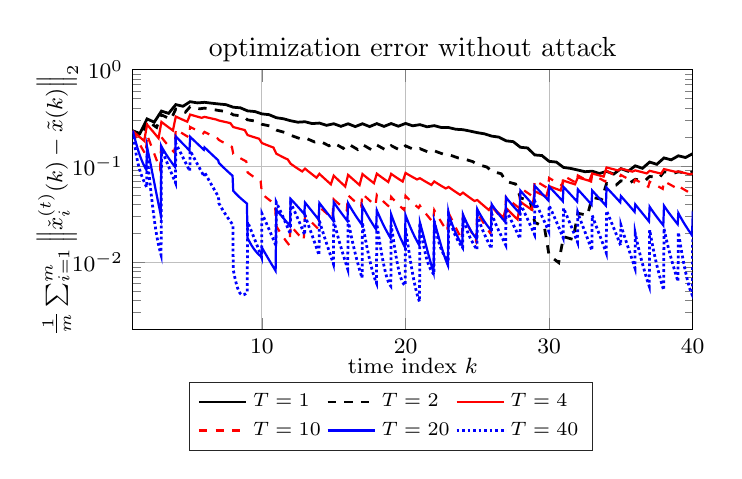
\begin{tikzpicture}
	\begin{semilogyaxis}
		[	width=2.8in,
		height=1.3in,
		at={(0in,1.8in)},
		scale only axis,
		xmin=1,
		xmax=40.0,
		ymin=0.002,
		ymax=1,
		title={optimization error without attack},
		title style={at={(axis description cs:0.5,1.1)},anchor=north},
		xlabel={\footnotesize time index $k$},
		ylabel={\footnotesize $\frac{1}{m}\sum_{i=1}^m \left\|\check{x}_i^{(t)}(k)-\tilde{x}(k)\right\|_2$},
		x label style={at={(axis description cs:0.5,-0.07)},anchor=north},
		y label style={at={(axis description cs:-0.08,.5)},anchor=south},
		xticklabel style = {font=\footnotesize},
		yticklabel style = {font=\footnotesize},
		axis background/.style={fill=white},
%		grid=both,
%		ytick={0,-0.5,-1,-1.5,-2,-2.5},
		xmajorgrids,
		ymajorgrids,
		legend style={at={(0.1,-0.2)}, anchor=north west, legend cell align=left, align=left, legend columns=3, draw=white!15!black, font=\scriptsize }]
		
		\addplot [color={black}, line width=1pt]
		table[row sep={\\}]
		{    0.0  0.0  \\
			0.5  0.0  \\
			1.0  0.2322129266725592  \\
			1.5  0.21760231632149898  \\
			2.0  0.3085867169430388  \\
			2.5  0.28564484654772776  \\
			3.0  0.372152272824885  \\
			3.5  0.35236525126579227  \\
			4.0  0.43443620488611595  \\
			4.5  0.4175195640641474  \\
			5.0  0.46580557333313616  \\
			5.5  0.4526015301412516  \\
			6.0  0.4588364151823898  \\
			6.5  0.44911197747142534  \\
			7.0  0.4409537557327197  \\
			7.5  0.43368152858859793  \\
			8.0  0.4080826841261844  \\
			8.5  0.4021904295361904  \\
			9.0  0.37390109774813846  \\
			9.5  0.3682559733906808  \\
			10.0  0.34788785279256634  \\
			10.5  0.3414558007008879  \\
			11.0  0.3175368475636841  \\
			11.5  0.30968254701262193  \\
			12.0  0.2952784914325442  \\
			12.5  0.28535622891552914  \\
			13.0  0.28835070513246963  \\
			13.5  0.27598973654045383  \\
			14.0  0.27938229524225733  \\
			14.5  0.2647588291016427  \\
			15.0  0.2749349270634828  \\
			15.5  0.25838365758674436  \\
			16.0  0.2746880968815045  \\
			16.5  0.2568380923689982  \\
			17.0  0.2750290748850784  \\
			17.5  0.25682083150777063  \\
			18.0  0.2758302403779585  \\
			18.5  0.2579649381999351  \\
			19.0  0.27610138130213496  \\
			19.5  0.2591972183114961  \\
			20.0  0.27690659264315226  \\
			20.5  0.26165626977311657  \\
			21.0  0.2691436553242999  \\
			21.5  0.25554466766020695  \\
			22.0  0.26287945181231037  \\
			22.5  0.251072006266062  \\
			23.0  0.2510458080730329  \\
			23.5  0.24103158393656413  \\
			24.0  0.23855611479073946  \\
			24.5  0.23054051686928423  \\
			25.0  0.22218304345802964  \\
			25.5  0.21590139180457327  \\
			26.0  0.20457934159288396  \\
			26.5  0.19973259633149307  \\
			27.0  0.1828052862138593  \\
			27.5  0.17915754855738553  \\
			28.0  0.15667782406033953  \\
			28.5  0.15408881635781815  \\
			29.0  0.13042097761187435  \\
			29.5  0.12847915948217703  \\
			30.0  0.11188087967947569  \\
			30.5  0.11006293848902587  \\
			31.0  0.0968104037281486  \\
			31.5  0.09445461765657964  \\
			32.0  0.09090396177686032  \\
			32.5  0.08736815303385544  \\
			33.0  0.08851141989319283  \\
			33.5  0.08370130914309315  \\
			34.0  0.08810151934579001  \\
			34.5  0.08259364656258121  \\
			35.0  0.09403851186874944  \\
			35.5  0.08824938431731326  \\
			36.0  0.10057274039436322  \\
			36.5  0.09470720619367747  \\
			37.0  0.11007483048870996  \\
			37.5  0.10426255735234986  \\
			38.0  0.12144129214672357  \\
			38.5  0.1160241971958511  \\
			39.0  0.127748266016483  \\
			39.5  0.12264495821214401  \\
			40.0  0.13446232190999538  \\
			40.5  0.1295531212068941  \\
			41.0  0.1402294973445284  \\
			41.5  0.13540012261399045  \\
			42.0  0.14495913634431987  \\
			42.5  0.14030395278866012  \\
			43.0  0.14548384882262208  \\
			43.5  0.14127770725511946  \\
			44.0  0.14334135674202658  \\
			44.5  0.13969259004308962  \\
			45.0  0.13167938744241375  \\
			45.5  0.12865762023393432  \\
			46.0  0.11415565720924915  \\
			46.5  0.111771240410599  \\
			47.0  0.09643954368246804  \\
			47.5  0.09472553539728806  \\
			48.0  0.07088661965113986  \\
			48.5  0.06980950358381667  \\
			49.0  0.0482688461125245  \\
			49.5  0.0475999315327435  \\
			50.0  0.03133721375022349  \\
	}
;\addlegendentry{$T=1$}
		
			\addplot [dashed, color={black}, line width=1pt]
		table[row sep={\\}]
		{      0.0  0.0  \\
			0.3333333333333333  0.0  \\
			0.6666666666666666  0.0  \\
			1.0  0.2322129266725592  \\
			1.3333333333333333  0.21760231632149898  \\
			1.6666666666666667  0.20520015611971407  \\
			2.0  0.2949408602143217  \\
			2.3333333333333335  0.2726661910521828  \\
			2.6666666666666665  0.2520606501468979  \\
			3.0  0.3404072623494206  \\
			3.3333333333333335  0.32218008509710305  \\
			3.6666666666666665  0.3052549411856701  \\
			4.0  0.39107912808310724  \\
			4.333333333333333  0.3764514238483103  \\
			4.666666666666667  0.36263358151126734  \\
			5.0  0.41319175705702343  \\
			5.333333333333333  0.40268263148027056  \\
			5.666666666666667  0.3926666988462429  \\
			6.0  0.399440542087569  \\
			6.333333333333333  0.3921793825506079  \\
			6.666666666666667  0.38504275747684896  \\
			7.0  0.377031936719279  \\
			7.333333333333333  0.37136849195968497  \\
			7.666666666666667  0.36569347492107224  \\
			8.0  0.34006046186947086  \\
			8.333333333333334  0.33489398236291223  \\
			8.666666666666666  0.32973952485394925  \\
			9.0  0.3018263334908224  \\
			9.333333333333334  0.29631804888918856  \\
			9.666666666666666  0.29094198435433943  \\
			10.0  0.27124258537167817  \\
			10.333333333333334  0.26484610049975627  \\
			10.666666666666666  0.2587485280033273  \\
			11.0  0.23619324489094584  \\
			11.333333333333334  0.22875824851686  \\
			11.666666666666666  0.22179153829971943  \\
			12.0  0.20889589201985656  \\
			12.333333333333334  0.20027015511970161  \\
			12.666666666666666  0.1922853661154652  \\
			13.0  0.19663683315014593  \\
			13.333333333333334  0.18685404435525166  \\
			13.666666666666666  0.17785095386708763  \\
			14.0  0.18265334274995423  \\
			14.333333333333334  0.1720635774548341  \\
			14.666666666666666  0.16227846384467148  \\
			15.0  0.17398516493021143  \\
			15.333333333333334  0.16286447620121167  \\
			15.666666666666666  0.15255437390643575  \\
			16.0  0.17020398806573564  \\
			16.333333333333332  0.1589480567651086  \\
			16.666666666666668  0.14850488214283153  \\
			17.0  0.1674311539834268  \\
			17.333333333333332  0.1566074360981126  \\
			17.666666666666668  0.14654600323257944  \\
			18.0  0.1653314669953542  \\
			18.333333333333332  0.15519040170253234  \\
			18.666666666666668  0.14577886822271055  \\
			19.0  0.1629520702189351  \\
			19.333333333333332  0.15371169203873872  \\
			19.666666666666668  0.1451453688563963  \\
			20.0  0.16221578099971554  \\
			20.333333333333332  0.15419854647791456  \\
			20.666666666666668  0.14676460800609062  \\
			21.0  0.1516791818008998  \\
			21.333333333333332  0.1446627219261247  \\
			21.666666666666668  0.13817693621255045  \\
			22.0  0.14401153207719294  \\
			22.333333333333332  0.1379321381715868  \\
			22.666666666666668  0.1323018465696724  \\
			23.0  0.1316421062319386  \\
			23.333333333333332  0.1264141730793923  \\
			23.666666666666668  0.12157304216928581  \\
			24.0  0.11952756036424532  \\
			24.333333333333332  0.1153220550838836  \\
			24.666666666666668  0.11139846125645218  \\
			25.0  0.10425099586517972  \\
			25.333333333333332  0.10086060451819634  \\
			25.666666666666668  0.09770117538299243  \\
			26.0  0.08845558851775237  \\
			26.333333333333332  0.08572359520933037  \\
			26.666666666666668  0.08316489212818484  \\
			27.0  0.06927118916321494  \\
			27.333333333333332  0.06711675537630774  \\
			27.666666666666668  0.06509403559930722  \\
			28.0  0.04670652108032669  \\
			28.333333333333332  0.04512636832062084  \\
			28.666666666666668  0.04364698747288711  \\
			29.0  0.025987233910629487  \\
			29.333333333333332  0.024700587553067404  \\
			29.666666666666668  0.023494033353475993  \\
			30.0  0.011739730694361123  \\
			30.333333333333332  0.010845655437088856  \\
			30.666666666666668  0.009938357569382869  \\
			31.0  0.018473973626540862  \\
			31.333333333333332  0.01789801070123666  \\
			31.666666666666668  0.01731801373557728  \\
			32.0  0.03240784961612415  \\
			32.333333333333336  0.031584930455354064  \\
			32.666666666666664  0.03078493568889533  \\
			33.0  0.047315018526382376  \\
			33.333333333333336  0.046225559252021035  \\
			33.666666666666664  0.04517545575149732  \\
			34.0  0.06604037587719112  \\
			34.333333333333336  0.06474762307149205  \\
			34.666666666666664  0.06350146384612775  \\
			35.0  0.07027391712733412  \\
			35.333333333333336  0.06893740667372628  \\
			35.666666666666664  0.06763086122534488  \\
			36.0  0.07285312302094157  \\
			36.333333333333336  0.07150491554283893  \\
			36.666666666666664  0.07018724532584465  \\
			37.0  0.07813713085993522  \\
			37.333333333333336  0.07674542469692676  \\
			37.666666666666664  0.07538689401522039  \\
			38.0  0.087195483051775  \\
			38.333333333333336  0.0856836999721413  \\
			38.666666666666664  0.08421210103465893  \\
			39.0  0.08715760985415666  \\
			39.333333333333336  0.08563512602594182  \\
			39.666666666666664  0.08414428118597189  \\
			40.0  0.0872495843682769  \\
			40.333333333333336  0.08565728663020654  \\
			40.666666666666664  0.08409994438519482  \\
			41.0  0.08672849277406115  \\
			41.333333333333336  0.08499329827648212  \\
			41.666666666666664  0.08331154949882165  \\
			42.0  0.08701104702024788  \\
			42.333333333333336  0.08510858339476075  \\
			42.666666666666664  0.08327365772904229  \\
			43.0  0.08522117596086021  \\
			43.333333333333336  0.08331879168565008  \\
			43.666666666666664  0.08148659485033732  \\
			44.0  0.08171876243619518  \\
			44.333333333333336  0.07993674191722427  \\
			44.666666666666664  0.07822867073509869  \\
			45.0  0.06963425815264225  \\
			45.333333333333336  0.068091502549694  \\
			45.666666666666664  0.06661177581864906  \\
			46.0  0.05327828643571803  \\
			46.333333333333336  0.051972769858632  \\
			46.666666666666664  0.05071448766944129  \\
			47.0  0.03803851162006767  \\
			47.333333333333336  0.037010710699383984  \\
			47.666666666666664  0.03600059966813404  \\
			48.0  0.02061879289400927  \\
			48.333333333333336  0.019586004157247656  \\
			48.666666666666664  0.018556855096939853  \\
			49.0  0.02260362233323225  \\
			49.333333333333336  0.021523642840695394  \\
			49.666666666666664  0.02046605075678528  \\
			50.0  0.03860949029097973  \\
	}
;\addlegendentry{$T=2$}
		
		\addplot [color={red}, line width=0.8pt]
		table[row sep={\\}]
		{  
			   0.0  0.0  \\
			  0.2  0.0  \\
			  0.4  0.0  \\
			  0.6  0.0  \\
			  0.8  0.0  \\
			  1.0  0.2322129266725592  \\
			  1.2  0.21760231632149898  \\
			  1.4  0.20520015611971407  \\
			  1.6  0.1935795049063174  \\
			  1.8  0.18254444406349454  \\
			  2.0  0.26966946216847065  \\
			  2.2  0.2484527491002941  \\
			  2.4  0.22925639055449346  \\
			  2.6  0.21134297351216913  \\
			  2.8  0.19459497313428273  \\
			  3.0  0.28742198043791184  \\
			  3.2  0.27244210980815625  \\
			  3.4  0.25879388073207427  \\
			  3.6  0.24596843479654282  \\
			  3.8  0.23393950648051576  \\
			  4.0  0.3267282331702911  \\
			  4.2  0.316265300517633  \\
			  4.4  0.3065007211452841  \\
			  4.6  0.2973486408768787  \\
			  4.8  0.28877968721594527  \\
			  5.0  0.34250388929518755  \\
			  5.2  0.33565642998411477  \\
			  5.4  0.32905419389845275  \\
			  5.6  0.3227098674353544  \\
			  5.8  0.31661864886514607  \\
			  6.0  0.324149941829695  \\
			  6.2  0.31914764318248695  \\
			  6.4  0.31421466675042325  \\
			  6.6  0.3093629919731744  \\
			  6.8  0.30458947158437916  \\
			  7.0  0.29699997580102927  \\
			  7.2  0.2923951991505316  \\
			  7.4  0.2878938507682766  \\
			  7.6  0.283467878364239  \\
			  7.8  0.2791038215404618  \\
			  8.0  0.2540258400695135  \\
			  8.2  0.2494321160580153  \\
			  8.4  0.24501648216314983  \\
			  8.6  0.24074079946310836  \\
			  8.8  0.23658363566377313  \\
			  9.0  0.20966185928126588  \\
			  9.2  0.20492576653478148  \\
			  9.4  0.20046677794893994  \\
			  9.6  0.1962208165745134  \\
			  9.8  0.19216132076711356  \\
			  10.0  0.17334150861350794  \\
			  10.2  0.16848678082099552  \\
			  10.4  0.16397160921552395  \\
			  10.6  0.1597299680493787  \\
			  10.8  0.15573096876531548  \\
			  11.0  0.1345033440087223  \\
			  11.2  0.12961825503030444  \\
			  11.4  0.12510095342286212  \\
			  11.6  0.12090312539529073  \\
			  11.8  0.11699695382668172  \\
			  12.0  0.10568275474382598  \\
			  12.2  0.10069434117751565  \\
			  12.4  0.0961110587403095  \\
			  12.6  0.09186639856717461  \\
			  12.8  0.08793237738085091  \\
			  13.0  0.09404138352723544  \\
			  13.2  0.08888936365314914  \\
			  13.4  0.0841869282946981  \\
			  13.6  0.07981462930320903  \\
			  13.8  0.07574147964834727  \\
			  14.0  0.08303149635691032  \\
			  14.2  0.07788911976187864  \\
			  14.4  0.07317055115172964  \\
			  14.6  0.06875894410111749  \\
			  14.8  0.06462830450492885  \\
			  15.0  0.07940637905895069  \\
			  15.2  0.07435729714461604  \\
			  15.4  0.0697249795468638  \\
			  15.6  0.06538175212947932  \\
			  15.8  0.06130183596500469  \\
			  16.0  0.08094267177801213  \\
			  16.2  0.0760619669460555  \\
			  16.4  0.07159632286368729  \\
			  16.6  0.0674097122219219  \\
			  16.8  0.06347464047506664  \\
			  17.0  0.08260880523541893  \\
			  17.2  0.07808951128220812  \\
			  17.4  0.07394199417180268  \\
			  17.6  0.07005877096343556  \\
			  17.8  0.06641582702289647  \\
			  18.0  0.08336734568179138  \\
			  18.2  0.07915759147249643  \\
			  18.4  0.0752986318395644  \\
			  18.6  0.07168797594878934  \\
			  18.8  0.06830244227319458  \\
			  19.0  0.08296869420951224  \\
			  19.2  0.07908445322446034  \\
			  19.4  0.07551856225761579  \\
			  19.6  0.07218655005428479  \\
			  19.8  0.06906607284940906  \\
			  20.0  0.08481742327944634  \\
			  20.2  0.08141687561694419  \\
			  20.4  0.07828527040156229  \\
			  20.6  0.07535761287819608  \\
			  20.8  0.07261726530178932  \\
			  21.0  0.0748485195701192  \\
			  21.2  0.07172588572961917  \\
			  21.4  0.06886605483277153  \\
			  21.6  0.0661990654762503  \\
			  21.8  0.06370952997180236  \\
			  22.0  0.0691962007410087  \\
			  22.2  0.06621993781817498  \\
			  22.4  0.06349106845209405  \\
			  22.6  0.06094567784355704  \\
			  22.8  0.05856805115243657  \\
			  23.0  0.060654106460722314  \\
			  23.2  0.05771896817531846  \\
			  23.4  0.0550429246066948  \\
			  23.6  0.052549210855621836  \\
			  23.8  0.05021982965360571  \\
			  24.0  0.052974113289507595  \\
			  24.2  0.05028849031385823  \\
			  24.4  0.04782931028526773  \\
			  24.6  0.04554106224357982  \\
			  24.8  0.043407598026027554  \\
			  25.0  0.04437637085854937  \\
			  25.2  0.04172968829667836  \\
			  25.4  0.03932471617360744  \\
			  25.6  0.03708768206061693  \\
			  25.8  0.034997026789466375  \\
			  26.0  0.03852898579093333  \\
			  26.2  0.03590052843846534  \\
			  26.4  0.033506813757527856  \\
			  26.6  0.031267796634085694  \\
			  26.8  0.02915860692977118  \\
			  27.0  0.036674790941550815  \\
			  27.2  0.03419346472860509  \\
			  27.4  0.03196277953255655  \\
			  27.6  0.029874705895630616  \\
			  27.8  0.027900400230839034  \\
			  28.0  0.04268165659036773  \\
			  28.2  0.04055008473827061  \\
			  28.4  0.03865101846629355  \\
			  28.6  0.036879387073493274  \\
			  28.8  0.035209620495509276  \\
			  29.0  0.054871691522433375  \\
			  29.2  0.052966562075520585  \\
			  29.4  0.05125735378974405  \\
			  29.6  0.049650085301278464  \\
			  29.8  0.048123678203677016  \\
			  30.0  0.06193774661352946  \\
			  30.2  0.06024483479036407  \\
			  30.4  0.058691237752462155  \\
			  30.6  0.0572125217876712  \\
			  30.8  0.05579533157647818  \\
			  31.0  0.0705894727184654  \\
			  31.2  0.06897398782134188  \\
			  31.4  0.06746069700572017  \\
			  31.6  0.06600502508008503  \\
			  31.8  0.0645972937947122  \\
			  32.0  0.07627047205547906  \\
			  32.2  0.07470130923676031  \\
			  32.4  0.07321091409849091  \\
			  32.6  0.07176550811089293  \\
			  32.8  0.07035846739642405  \\
			  33.0  0.08376333616693422  \\
			  33.2  0.08216963488571212  \\
			  33.4  0.08064474318451254  \\
			  33.6  0.07915893832808184  \\
			  33.8  0.07770612741560544  \\
			  34.0  0.09676811860706129  \\
			  34.2  0.09500435723253114  \\
			  34.4  0.09332709665802112  \\
			  34.6  0.09168619272697172  \\
			  34.8  0.09007339269373227  \\
			  35.0  0.09415889553182867  \\
			  35.2  0.09244575835455117  \\
			  35.4  0.09078631586672624  \\
			  35.6  0.08916134885261894  \\
			  35.8  0.08756860433060999  \\
			  36.0  0.09013318629772721  \\
			  36.2  0.08853441709893932  \\
			  36.4  0.0869785998189803  \\
			  36.6  0.08545523493667355  \\
			  36.8  0.08396360865135942  \\
			  37.0  0.08927210154623726  \\
			  37.2  0.0877885243920161  \\
			  37.4  0.08633353467274014  \\
			  37.6  0.08490404703253736  \\
			  37.8  0.08349997217514527  \\
			  38.0  0.09299296025205805  \\
			  38.2  0.09148106978232312  \\
			  38.4  0.09000401849048312  \\
			  38.6  0.08854829967964707  \\
			  38.8  0.08711326694107112  \\
			  39.0  0.08777969195129946  \\
			  39.2  0.08635348436113316  \\
			  39.4  0.08494507098530758  \\
			  39.6  0.08355395063179265  \\
			  39.8  0.08218377172935853  \\
			  40.0  0.08323957298469321  \\
			  40.2  0.08184359332704225  \\
			  40.4  0.0804615498460398  \\
			  40.6  0.07910080262491477  \\
			  40.8  0.0777650123481748  \\
			  41.0  0.07857055925137928  \\
			  41.2  0.07712718094499821  \\
			  41.4  0.07571080733229989  \\
			  41.6  0.07432592768795813  \\
			  41.8  0.07297664105203426  \\
			  42.0  0.07527648713084205  \\
			  42.2  0.07372358828329052  \\
			  42.4  0.0722172114451953  \\
			  42.6  0.07076252966243608  \\
			  42.8  0.0693591824474599  \\
			  43.0  0.0706178967957685  \\
			  43.2  0.0690856312972351  \\
			  43.4  0.06760861511864188  \\
			  43.6  0.06619268822744422  \\
			  43.8  0.06483537252441975  \\
			  44.0  0.06467619792119479  \\
			  44.2  0.06327738851232058  \\
			  44.4  0.06193576310907545  \\
			  44.6  0.060653831825727596  \\
			  44.8  0.05942834838137375  \\
			  45.0  0.05109279384742801  \\
			  45.2  0.04988586899847225  \\
			  45.4  0.04873526521235182  \\
			  45.6  0.047644466228888266  \\
			  45.8  0.04661038910520605  \\
			  46.0  0.03494470205835775  \\
			  46.2  0.03383100807864897  \\
			  46.4  0.03277902617725121  \\
			  46.6  0.0317931973415651  \\
			  46.8  0.030871848154834767  \\
			  47.0  0.022317262915921898  \\
			  47.2  0.021233082383623692  \\
			  47.4  0.020209249626670454  \\
			  47.6  0.019258365986456638  \\
			  47.8  0.018375468230338133  \\
			  48.0  0.021524041255661194  \\
			  48.2  0.02036002567225296  \\
			  48.4  0.019300136193239063  \\
			  48.6  0.018300623051814013  \\
			  48.8  0.017345680971726826  \\
			  49.0  0.03637149762785138  \\
			  49.2  0.0352515136804399  \\
			  49.4  0.03422391723529696  \\
			  49.6  0.03324066786346641  \\
			  49.8  0.03229076137317546  \\
			  50.0  0.05324998352454997  \\
		}
		;\addlegendentry{$T=4$}
		
		\addplot [dashed, color={red}, line width=0.8pt]
		table[row sep={\\}]
		{
		     0.0  0.0  \\
		    0.09090909090909091  0.0  \\
		    0.18181818181818182  0.0  \\
		    0.2727272727272727  0.0  \\
		    0.36363636363636365  0.0  \\
		    0.45454545454545453  0.0  \\
		    0.5454545454545454  0.0  \\
		    0.6363636363636364  0.0  \\
		    0.7272727272727273  0.0  \\
		    0.8181818181818182  0.0  \\
		    0.9090909090909091  0.0  \\
		    1.0  0.2322129266725592  \\
		    1.0909090909090908  0.21760231632149898  \\
		    1.1818181818181819  0.20520015611971407  \\
		    1.2727272727272727  0.1935795049063174  \\
		    1.3636363636363635  0.18254444406349454  \\
		    1.4545454545454546  0.17217244094692577  \\
		    1.5454545454545454  0.1625605532277158  \\
		    1.6363636363636365  0.15375598944029462  \\
		    1.7272727272727273  0.1457462353920317  \\
		    1.8181818181818181  0.13847977732390562  \\
		    1.9090909090909092  0.13189114081117817  \\
		    2.0  0.2104130737837304  \\
		    2.090909090909091  0.19366916589902985  \\
		    2.1818181818181817  0.17885478084833747  \\
		    2.272727272727273  0.16506931858071108  \\
		    2.3636363636363638  0.15214355466565788  \\
		    2.4545454545454546  0.14006999985018054  \\
		    2.5454545454545454  0.12886327751415846  \\
		    2.6363636363636362  0.11851741470815158  \\
		    2.727272727272727  0.10899645149955617  \\
		    2.8181818181818183  0.10024507227172502  \\
		    2.909090909090909  0.09220330536428438  \\
		    3.0  0.19988655437226596  \\
		    3.090909090909091  0.19162490944217744  \\
		    3.1818181818181817  0.18420295067907913  \\
		    3.272727272727273  0.1771748747920585  \\
		    3.3636363636363638  0.1705199688353892  \\
		    3.4545454545454546  0.16424024162929632  \\
		    3.5454545454545454  0.15833445435280405  \\
		    3.6363636363636362  0.15279299606739957  \\
		    3.727272727272727  0.1475956614612212  \\
		    3.8181818181818183  0.14271673603016724  \\
		    3.909090909090909  0.13813118390126444  \\
		    4.0  0.24196039386131707  \\
		    4.090909090909091  0.2368403932741632  \\
		    4.181818181818182  0.23199920774060703  \\
		    4.2727272727272725  0.22733253905644146  \\
		    4.363636363636363  0.2228315624434706  \\
		    4.454545454545454  0.21848639494644553  \\
		    4.545454545454546  0.21428777455843592  \\
		    4.636363636363637  0.2102266060814845  \\
		    4.7272727272727275  0.20629392960262213  \\
		    4.818181818181818  0.20248144169063295  \\
		    4.909090909090909  0.1987817815258018  \\
		    5.0  0.2547211372801192  \\
		    5.090909090909091  0.25073423700236086  \\
		    5.181818181818182  0.24687612259661074  \\
		    5.2727272727272725  0.24307451160488658  \\
		    5.363636363636363  0.23932326403300752  \\
		    5.454545454545454  0.23562178122944052  \\
		    5.545454545454546  0.23197229968628563  \\
		    5.636363636363637  0.2283768017202665  \\
		    5.7272727272727275  0.22483605287229738  \\
		    5.818181818181818  0.22135024459332822  \\
		    5.909090909090909  0.2179196264877115  \\
		    6.0  0.22632704098598322  \\
		    6.090909090909091  0.22274565455603215  \\
		    6.181818181818182  0.21929511346983535  \\
		    6.2727272727272725  0.2159072647497471  \\
		    6.363636363636363  0.2125702057757599  \\
		    6.454545454545454  0.20928372833734257  \\
		    6.545454545454546  0.2060507938094208  \\
		    6.636363636363637  0.20287367986502736  \\
		    6.7272727272727275  0.19975281967800287  \\
		    6.818181818181818  0.1966875618361367  \\
		    6.909090909090909  0.1936770604746413  \\
		    7.0  0.18677396185456308  \\
		    7.090909090909091  0.18348140995807025  \\
		    7.181818181818182  0.18034001125388519  \\
		    7.2727272727272725  0.17729680426129965  \\
		    7.363636363636363  0.17433249222992694  \\
		    7.454545454545454  0.17144372989467574  \\
		    7.545454545454546  0.168630335557322  \\
		    7.636363636363637  0.16589130477616534  \\
		    7.7272727272727275  0.16322394341769464  \\
		    7.818181818181818  0.16062467657727295  \\
		    7.909090909090909  0.15808993119884676  \\
		    8.0  0.13391497265880992  \\
		    8.090909090909092  0.13125816811506527  \\
		    8.181818181818182  0.12872083310273227  \\
		    8.272727272727273  0.12629602252498154  \\
		    8.363636363636363  0.12396747033248035  \\
		    8.454545454545455  0.12172877993748538  \\
		    8.545454545454545  0.11957527566641331  \\
		    8.636363636363637  0.11750210796978745  \\
		    8.727272727272727  0.11550376000782285  \\
		    8.818181818181818  0.11357447226463012  \\
		    8.909090909090908  0.11170877904869962  \\
		    9.0  0.08588623764499492  \\
		    9.090909090909092  0.08387776357900899  \\
		    9.181818181818182  0.08197091491008764  \\
		    9.272727272727273  0.08016665137010114  \\
		    9.363636363636363  0.07845456476270844  \\
		    9.454545454545455  0.07682857862381814  \\
		    9.545454545454545  0.07528339911303299  \\
		    9.636363636363637  0.07381356130727633  \\
		    9.727272727272727  0.07241307224592859  \\
		    9.818181818181818  0.07107580637270709  \\
		    9.909090909090908  0.0697959947720297  \\
		    10.0  0.051658738294215904  \\
		    10.090909090909092  0.05020735573254086  \\
		    10.181818181818182  0.04882521763794114  \\
		    10.272727272727273  0.047533581283793674  \\
		    10.363636363636363  0.04632432846307883  \\
		    10.454545454545455  0.04519157384103235  \\
		    10.545454545454545  0.044129790543176346  \\
		    10.636363636363637  0.043133556758183624  \\
		    10.727272727272727  0.0421972279546072  \\
		    10.818181818181818  0.041315131315104045  \\
		    10.909090909090908  0.04048191988783209  \\
		    11.0  0.023741927128529686  \\
		    11.090909090909092  0.02258488431243565  \\
		    11.181818181818182  0.021468743097164053  \\
		    11.272727272727273  0.020430116290937585  \\
		    11.363636363636363  0.019469882026620176  \\
		    11.454545454545455  0.018583127076005186  \\
		    11.545454545454545  0.01776446181288698  \\
		    11.636363636363637  0.017009132346946777  \\
		    11.727272727272727  0.016312547257127375  \\
		    11.818181818181818  0.01567014635490115  \\
		    11.909090909090908  0.015077539805772415  \\
		    12.0  0.024141507871737147  \\
		    12.090909090909092  0.02324116392219172  \\
		    12.181818181818182  0.022396660089693505  \\
		    12.272727272727273  0.021591427027547933  \\
		    12.363636363636363  0.020824971321646343  \\
		    12.454545454545455  0.020096371191109443  \\
		    12.545454545454545  0.019404640348572255  \\
		    12.636363636363637  0.018748353266206018  \\
		    12.727272727272727  0.01812530457716661  \\
		    12.818181818181818  0.017532881721914136  \\
		    12.909090909090908  0.01696859114855013  \\
		    13.0  0.03081350064692413  \\
		    13.090909090909092  0.029767789747176834  \\
		    13.181818181818182  0.028804547728926228  \\
		    13.272727272727273  0.02787951812111847  \\
		    13.363636363636363  0.026989861332713916  \\
		    13.454545454545455  0.02613623235261882  \\
		    13.545454545454545  0.025319243665127538  \\
		    13.636363636363637  0.02453862656953862  \\
		    13.727272727272727  0.02379305770643679  \\
		    13.818181818181818  0.023080521570929657  \\
		    13.909090909090908  0.022398783239987296  \\
		    14.0  0.03772678561497265  \\
		    14.090909090909092  0.03662771622312031  \\
		    14.181818181818182  0.03560638819422813  \\
		    14.272727272727273  0.03462302050237583  \\
		    14.363636363636363  0.033676016149833975  \\
		    14.454545454545455  0.032765478632267885  \\
		    14.545454545454545  0.03189119196515433  \\
		    14.636363636363637  0.031052185628552914  \\
		    14.727272727272727  0.03024675558187438  \\
		    14.818181818181818  0.029472788862536934  \\
		    14.909090909090908  0.02872810002813786  \\
		    15.0  0.04505647330670822  \\
		    15.090909090909092  0.043786489308361036  \\
		    15.181818181818182  0.04260832980257582  \\
		    15.272727272727273  0.041473918028577986  \\
		    15.363636363636363  0.040380526973215265  \\
		    15.454545454545455  0.03932807841943389  \\
		    15.545454545454545  0.038316595746245304  \\
		    15.636363636363637  0.0373452410097812  \\
		    15.727272727272727  0.0364121772038343  \\
		    15.818181818181818  0.035515020482597214  \\
		    15.909090909090908  0.03465131053508116  \\
		    16.0  0.049777388025796065  \\
		    16.09090909090909  0.04829708230453595  \\
		    16.181818181818183  0.04692617424124201  \\
		    16.272727272727273  0.04561244996449331  \\
		    16.363636363636363  0.044351461545662996  \\
		    16.454545454545453  0.043142634657205296  \\
		    16.545454545454547  0.041985911273843234  \\
		    16.636363636363637  0.040880180976910034  \\
		    16.727272727272727  0.03982294087339182  \\
		    16.818181818181817  0.03881092599487498  \\
		    16.90909090909091  0.037840789758378617  \\
		    17.0  0.051560110108927214  \\
		    17.09090909090909  0.04999982442247114  \\
		    17.181818181818183  0.048552092389714425  \\
		    17.272727272727273  0.047168524891771736  \\
		    17.363636363636363  0.04584311955081256  \\
		    17.454545454545453  0.04457451506980157  \\
		    17.545454545454547  0.04336213471097716  \\
		    17.636363636363637  0.04220441753088112  \\
		    17.727272727272727  0.04109846394132819  \\
		    17.818181818181817  0.04004068005708022  \\
		    17.90909090909091  0.0390274568420883  \\
		    18.0  0.050189605721436374  \\
		    18.09090909090909  0.04856118968780765  \\
		    18.181818181818183  0.0470608804015458  \\
		    18.272727272727273  0.04563136955590827  \\
		    18.363636363636363  0.044265794085485734  \\
		    18.454545454545453  0.042962844305468456  \\
		    18.545454545454547  0.04172226939680746  \\
		    18.636363636363637  0.04054263838289079  \\
		    18.727272727272727  0.03942081507392742  \\
		    18.818181818181817  0.03835272826377759  \\
		    18.90909090909091  0.03733422485840164  \\
		    19.0  0.047854773554113474  \\
		    19.09090909090909  0.04618795904844441  \\
		    19.181818181818183  0.04465961998120021  \\
		    19.272727272727273  0.04320978955293726  \\
		    19.363636363636363  0.04183028345708759  \\
		    19.454545454545453  0.04051934424215196  \\
		    19.545454545454547  0.0392767403975345  \\
		    19.636363636363637  0.03810083914145997  \\
		    19.727272727272727  0.036987933998178686  \\
		    19.818181818181817  0.03593330066712683  \\
		    19.90909090909091  0.034932278368020826  \\
		    20.0  0.049036882056711716  \\
		    20.09090909090909  0.04745398388321265  \\
		    20.181818181818183  0.046003772294378936  \\
		    20.272727272727273  0.04462860214717112  \\
		    20.363636363636363  0.043321865384020004  \\
		    20.454545454545453  0.04208116064489612  \\
		    20.545454545454547  0.04090496205939472  \\
		    20.636363636363637  0.03979082395269201  \\
		    20.727272727272727  0.03873495979334663  \\
		    20.818181818181817  0.037732879821378636  \\
		    20.90909090909091  0.036780104562479786  \\
		    21.0  0.03881455590699259  \\
		    21.09090909090909  0.03711817952931546  \\
		    21.181818181818183  0.03559769576436426  \\
		    21.272727272727273  0.034160497193265596  \\
		    21.363636363636363  0.03280083834468383  \\
		    21.454545454545453  0.03151795759526588  \\
		    21.545454545454547  0.030313510405648766  \\
		    21.636363636363637  0.0291873753734856  \\
		    21.727272727272727  0.02813606456933142  \\
		    21.818181818181817  0.027154237434458148  \\
		    21.90909090909091  0.026236452609469333  \\
		    22.0  0.03486219567117429  \\
		    22.09090909090909  0.03296140146281049  \\
		    22.181818181818183  0.03127657274767114  \\
		    22.272727272727273  0.029691536153413727  \\
		    22.363636363636363  0.028187978808770605  \\
		    22.454545454545453  0.026765434846658484  \\
		    22.545454545454547  0.025427620083869822  \\
		    22.636363636363637  0.02417595312608868  \\
		    22.727272727272727  0.02300805740199406  \\
		    22.818181818181817  0.02191933908951976  \\
		    22.90909090909091  0.020904766608542225  \\
		    23.0  0.032591955597218274  \\
		    23.09090909090909  0.03049534648588721  \\
		    23.181818181818183  0.028670716183502653  \\
		    23.272727272727273  0.026954556100606732  \\
		    23.363636363636363  0.025312717025915952  \\
		    23.454545454545453  0.023745460177357958  \\
		    23.545454545454547  0.022260342715963537  \\
		    23.636363636363637  0.02086214498836102  \\
		    23.727272727272727  0.01955115178002911  \\
		    23.818181818181817  0.018324923775854682  \\
		    23.90909090909091  0.017180117364660213  \\
		    24.0  0.030735853854875872  \\
		    24.09090909090909  0.02879539168708839  \\
		    24.181818181818183  0.027112541251327227  \\
		    24.272727272727273  0.02553520860370832  \\
		    24.363636363636363  0.024029511158223927  \\
		    24.454545454545453  0.02259497311431494  \\
		    24.545454545454547  0.021237957570761096  \\
		    24.636363636363637  0.019962356924875687  \\
		    24.727272727272727  0.01876816680173788  \\
		    24.818181818181817  0.017653101042642474  \\
		    24.90909090909091  0.016614182251793532  \\
		    25.0  0.032838347477408845  \\
		    25.09090909090909  0.031029831535292682  \\
		    25.181818181818183  0.029487757996977625  \\
		    25.272727272727273  0.028048523107005254  \\
		    25.363636363636363  0.02667619990661484  \\
		    25.454545454545453  0.025370212684181905  \\
		    25.545454545454547  0.024137222337374215  \\
		    25.636363636363637  0.02298146723699003  \\
		    25.727272727272727  0.021903105912604845  \\
		    25.818181818181817  0.020899737924642253  \\
		    25.90909090909091  0.01996805759856153  \\
		    26.0  0.03830328004943871  \\
		    26.09090909090909  0.036711858444735374  \\
		    26.181818181818183  0.0353547226219312  \\
		    26.272727272727273  0.03408785651048976  \\
		    26.363636363636363  0.03288159388366809  \\
		    26.454545454545453  0.03173427783554763  \\
		    26.545454545454547  0.030650005620880688  \\
		    26.636363636363637  0.02963087039875895  \\
		    26.727272727272727  0.02867562918353596  \\
		    26.818181818181817  0.027781124533730172  \\
		    26.90909090909091  0.026943776128445594  \\
		    27.0  0.04763473097476029  \\
		    27.09090909090909  0.0461883393159677  \\
		    27.181818181818183  0.044938300490239176  \\
		    27.272727272727273  0.04375694414424316  \\
		    27.363636363636363  0.042620968340987976  \\
		    27.454545454545453  0.04152898540258799  \\
		    27.545454545454547  0.04048453402892489  \\
		    27.636363636363637  0.03948955585446395  \\
		    27.727272727272727  0.03854313233327933  \\
		    27.818181818181817  0.03764277106824381  \\
		    27.90909090909091  0.03678574266760016  \\
		    28.0  0.05956103015984243  \\
		    28.09090909090909  0.05811926188265045  \\
		    28.181818181818183  0.05683512659987334  \\
		    28.272727272727273  0.05560418334898828  \\
		    28.363636363636363  0.05440791230410277  \\
		    28.454545454545453  0.0532451972482982  \\
		    28.545454545454547  0.052119409811912785  \\
		    28.636363636363637  0.05103258792649143  \\
		    28.727272727272727  0.04998427217089199  \\
		    28.818181818181817  0.048972713070582506  \\
		    28.90909090909091  0.047996063429795566  \\
		    29.0  0.07133799462287009  \\
		    29.09090909090909  0.06984657631747422  \\
		    29.181818181818183  0.0684909790414102  \\
		    29.272727272727273  0.0671779964616528  \\
		    29.363636363636363  0.06589286102895801  \\
		    29.454545454545453  0.06463511873586077  \\
		    29.545454545454547  0.06340798135367036  \\
		    29.636363636363637  0.06221358174904095  \\
		    29.727272727272727  0.061052002280333105  \\
		    29.818181818181817  0.05992222432655405  \\
		    29.90909090909091  0.05882308171111416  \\
		    30.0  0.07523482340448934  \\
		    30.09090909090909  0.07380532650200185  \\
		    30.181818181818183  0.07247569418215695  \\
		    30.272727272727273  0.07117776242827933  \\
		    30.363636363636363  0.06990131345953453  \\
		    30.454545454545453  0.0686460472772134  \\
		    30.545454545454547  0.06741434426638103  \\
		    30.636363636363637  0.06620782898921744  \\
		    30.727272727272727  0.06502670080540544  \\
		    30.818181818181817  0.06387045670663734  \\
		    30.90909090909091  0.0627385694638683  \\
		    31.0  0.07943952755296775  \\
		    31.09090909090909  0.07801458008183053  \\
		    31.181818181818183  0.07666234340038898  \\
		    31.272727272727273  0.07533724297086725  \\
		    31.363636363636363  0.07403181025016105  \\
		    31.454545454545453  0.07274576965712985  \\
		    31.545454545454547  0.07148079893385513  \\
		    31.636363636363637  0.07023809189652479  \\
		    31.727272727272727  0.06901789820158612  \\
		    31.818181818181817  0.06781998044548261  \\
		    31.90909090909091  0.06664404551992602  \\
		    32.0  0.0799287605466248  \\
		    32.09090909090909  0.07853308674944916  \\
		    32.18181818181818  0.07719431154862307  \\
		    32.27272727272727  0.0758778907622674  \\
		    32.36363636363637  0.07457956434801272  \\
		    32.45454545454545  0.07329948468120791  \\
		    32.54545454545455  0.07203894900820122  \\
		    32.63636363636363  0.07079886518331847  \\
		    32.72727272727273  0.06957947795792299  \\
		    32.81818181818182  0.06838067068163703  \\
		    32.90909090909091  0.06720225417435961  \\
		    33.0  0.08191495152062132  \\
		    33.09090909090909  0.08052262867185216  \\
		    33.18181818181818  0.07917973977686257  \\
		    33.27272727272727  0.07785841814947446  \\
		    33.36363636363637  0.07655451190466658  \\
		    33.45454545454545  0.07526801655871296  \\
		    33.54545454545455  0.07400001049432546  \\
		    33.63636363636363  0.07275129444845123  \\
		    33.72727272727273  0.07152216356112395  \\
		    33.81818181818182  0.0703126418671272  \\
		    33.90909090909091  0.0691226924949422  \\
		    34.0  0.08924817773548126  \\
		    34.09090909090909  0.08775527253958108  \\
		    34.18181818181818  0.08632565560482262  \\
		    34.27272727272727  0.08491575442743539  \\
		    34.36363636363637  0.08352006628164861  \\
		    34.45454545454545  0.08213900734303231  \\
		    34.54545454545455  0.08077463847327047  \\
		    34.63636363636363  0.07942863070138302  \\
		    34.72727272727273  0.07810187881172183  \\
		    34.81818181818182  0.0767948473879975  \\
		    34.90909090909091  0.0755078867471153  \\
		    35.0  0.0808184257187342  \\
		    35.09090909090909  0.07944696896652119  \\
		    35.18181818181818  0.07811090069562351  \\
		    35.27272727272727  0.07679444733733444  \\
		    35.36363636363637  0.07549695727596935  \\
		    35.45454545454545  0.0742186736534938  \\
		    35.54545454545455  0.07295983848663763  \\
		    35.63636363636363  0.07172044052380243  \\
		    35.72727272727273  0.07050025752634052  \\
		    35.81818181818182  0.06929898997063205  \\
		    35.90909090909091  0.06811635477192458  \\
		    36.0  0.07233876529686553  \\
		    36.09090909090909  0.07112456883227247  \\
		    36.18181818181818  0.06993389868929813  \\
		    36.27272727272727  0.06875870400962512  \\
		    36.36363636363637  0.06760041761687101  \\
		    36.45454545454545  0.06645937532625072  \\
		    36.54545454545455  0.06533554790483848  \\
		    36.63636363636363  0.06422877042151434  \\
		    36.72727272727273  0.06313881541740539  \\
		    36.81818181818182  0.062065424975678816  \\
		    36.90909090909091  0.06100833297020159  \\
		    37.0  0.06879500548699234  \\
		    37.09090909090909  0.06762841295608187  \\
		    37.18181818181818  0.06648596544922662  \\
		    37.27272727272727  0.0653603339735286  \\
		    37.36363636363637  0.06425288078048398  \\
		    37.45454545454545  0.06316352283995118  \\
		    37.54545454545455  0.06209208694724261  \\
		    37.63636363636363  0.06103837780600973  \\
		    37.72727272727273  0.06000208176331257  \\
		    37.81818181818182  0.05898282018528287  \\
		    37.90909090909091  0.05798022610184059  \\
		    38.0  0.06965274586565974  \\
		    38.09090909090909  0.06845134461738779  \\
		    38.18181818181818  0.067283278718559  \\
		    38.27272727272727  0.06613374145016838  \\
		    38.36363636363637  0.06500361202106197  \\
		    38.45454545454545  0.06389282233315974  \\
		    38.54545454545455  0.06280119974749894  \\
		    38.63636363636363  0.061728512645384655  \\
		    38.72727272727273  0.06067442310646035  \\
		    38.81818181818182  0.05963851977748208  \\
		    38.90909090909091  0.058620374086739  \\
		    39.0  0.06193768753002593  \\
		    39.09090909090909  0.06078896611600119  \\
		    39.18181818181818  0.05967067539442553  \\
		    39.27272727272727  0.05857297968390826  \\
		    39.36363636363637  0.05749978505264658  \\
		    39.45454545454545  0.05645137141086803  \\
		    39.54545454545455  0.0554270080788197  \\
		    39.63636363636363  0.0544256663581904  \\
		    39.72727272727273  0.05344618777200635  \\
		    39.81818181818182  0.0524873976645942  \\
		    39.90909090909091  0.0515481911770626  \\
		    40.0  0.05641541211931075  \\
		    40.09090909090909  0.05517861233674071  \\
		    40.18181818181818  0.05399421682378471  \\
		    40.27272727272727  0.05284354720926563  \\
		    40.36363636363637  0.0517284686507509  \\
		    40.45454545454545  0.05064865748930861  \\
		    40.54545454545455  0.049603483512870666  \\
		    40.63636363636363  0.04859171195661726  \\
		    40.72727272727273  0.047611388847007254  \\
		    40.81818181818182  0.046660297153421564  \\
		    40.90909090909091  0.045736364431587455  \\
		    41.0  0.051747945289895236  \\
		    41.09090909090909  0.050279259913344095  \\
		    41.18181818181818  0.04891323948839404  \\
		    41.27272727272727  0.047604514113415965  \\
		    41.36363636363637  0.04635208569350493  \\
		    41.45454545454545  0.045154910553366734  \\
		    41.54545454545455  0.04401261119586542  \\
		    41.63636363636363  0.04292370901351677  \\
		    41.72727272727273  0.04188498971279026  \\
		    41.81818181818182  0.04089243388870842  \\
		    41.90909090909091  0.03994217306008505  \\
		    42.0  0.047825328733814704  \\
		    42.09090909090909  0.0461807157140827  \\
		    42.18181818181818  0.044673071790835774  \\
		    42.27272727272727  0.0432456189353032  \\
		    42.36363636363637  0.04189089342245166  \\
		    42.45454545454545  0.04060673964258155  \\
		    42.54545454545455  0.03939281326982054  \\
		    42.63636363636363  0.038247404427481486  \\
		    42.72727272727273  0.03716647975089589  \\
		    42.81818181818182  0.03614485488923474  \\
		    42.90909090909091  0.03517745667494449  \\
		    43.0  0.041238345415362386  \\
		    43.09090909090909  0.03968347572309938  \\
		    43.18181818181818  0.03826485669768422  \\
		    43.27272727272727  0.036930193335386316  \\
		    43.36363636363637  0.03567058826808276  \\
		    43.45454545454545  0.034483398781836205  \\
		    43.54545454545455  0.03336774399457733  \\
		    43.63636363636363  0.032321433236771106  \\
		    43.72727272727273  0.031340153675419  \\
		    43.81818181818182  0.03041856013593139  \\
		    43.90909090909091  0.029551435221407168  \\
		    44.0  0.03378750590868744  \\
		    44.09090909090909  0.03242621923840961  \\
		    44.18181818181818  0.03119073134671263  \\
		    44.27272727272727  0.03003245947362314  \\
		    44.36363636363637  0.02894368414444558  \\
		    44.45454545454545  0.027922148286634158  \\
		    44.54545454545455  0.02696681709393839  \\
		    44.63636363636363  0.02607553277273909  \\
		    44.72727272727273  0.025244378803722628  \\
		    44.81818181818182  0.024468490595816222  \\
		    44.90909090909091  0.02374298736299804  \\
		    45.0  0.023172066029290908  \\
		    45.09090909090909  0.0218181922426289  \\
		    45.18181818181818  0.02062031017543717  \\
		    45.27272727272727  0.019497118417002593  \\
		    45.36363636363637  0.018435101362667353  \\
		    45.45454545454545  0.017433940756214013  \\
		    45.54545454545455  0.016496871025907852  \\
		    45.63636363636363  0.015625467680513132  \\
		    45.72727272727273  0.014818140122934571  \\
		    45.81818181818182  0.014071407042328891  \\
		    45.90909090909091  0.013381455697326345  \\
		    46.0  0.021430698275925895  \\
		    46.09090909090909  0.020068657045211737  \\
		    46.18181818181818  0.018914711096123738  \\
		    46.27272727272727  0.017834717633366786  \\
		    46.36363636363637  0.016799001285492485  \\
		    46.45454545454545  0.015808462504422683  \\
		    46.54545454545455  0.014869796656662248  \\
		    46.63636363636363  0.013987314135417712  \\
		    46.72727272727273  0.0131618985248805  \\
		    46.81818181818182  0.012392445377923542  \\
		    46.90909090909091  0.011677208109057991  \\
		    47.0  0.027066834231497184  \\
		    47.09090909090909  0.02600821897085365  \\
		    47.18181818181818  0.025108660130729016  \\
		    47.27272727272727  0.024263027147792136  \\
		    47.36363636363637  0.023451933499022876  \\
		    47.45454545454545  0.02267412051359152  \\
		    47.54545454545455  0.021933569957429608  \\
		    47.63636363636363  0.021233016516921135  \\
		    47.72727272727273  0.020572166787038267  \\
		    47.81818181818182  0.019949011326858813  \\
		    47.90909090909091  0.01936136580810591  \\
		    48.0  0.0433806590872678  \\
		    48.09090909090909  0.042319238504068275  \\
		    48.18181818181818  0.04138027239379468  \\
		    48.27272727272727  0.04047550765614111  \\
		    48.36363636363637  0.03959031086169492  \\
		    48.45454545454545  0.03872421073627114  \\
		    48.54545454545455  0.03788135679237256  \\
		    48.63636363636363  0.03706486348577253  \\
		    48.72727272727273  0.03627528070940149  \\
		    48.81818181818182  0.035511749297943644  \\
		    48.90909090909091  0.03477326861122613  \\
		    49.0  0.056901548859897934  \\
		    49.09090909090909  0.05573113269925897  \\
		    49.18181818181818  0.05466182826218461  \\
		    49.27272727272727  0.05362133600204083  \\
		    49.36363636363637  0.052598384686912  \\
		    49.45454545454545  0.05159284495227077  \\
		    49.54545454545455  0.05060800538758537  \\
		    49.63636363636363  0.049646240839725554  \\
		    49.72727272727273  0.04870801415831566  \\
		    49.81818181818182  0.04779280385710589  \\
		    49.90909090909091  0.046900032995247136  \\
		    50.0  0.06842326353828994  \\
		}
		;\addlegendentry{{$T=10$}}
		
		
		
		\addplot[ color={blue}, line width=0.8pt]
		table[row sep={\\}]
		{ 0.0  0.0  \\
			0.047619047619047616  0.0  \\
			0.09523809523809523  0.0  \\
			0.14285714285714285  0.0  \\
			0.19047619047619047  0.0  \\
			0.23809523809523808  0.0  \\
			0.2857142857142857  0.0  \\
			0.3333333333333333  0.0  \\
			0.38095238095238093  0.0  \\
			0.42857142857142855  0.0  \\
			0.47619047619047616  0.0  \\
			0.5238095238095238  0.0  \\
			0.5714285714285714  0.0  \\
			0.6190476190476191  0.0  \\
			0.6666666666666666  0.0  \\
			0.7142857142857143  0.0  \\
			0.7619047619047619  0.0  \\
			0.8095238095238095  0.0  \\
			0.8571428571428571  0.0  \\
			0.9047619047619048  0.0  \\
			0.9523809523809523  0.0  \\
			1.0  0.2322129266725592  \\
			1.0476190476190477  0.21760231632149898  \\
			1.0952380952380953  0.20520015611971407  \\
			1.1428571428571428  0.1935795049063174  \\
			1.1904761904761905  0.18254444406349454  \\
			1.2380952380952381  0.17217244094692577  \\
			1.2857142857142858  0.1625605532277158  \\
			1.3333333333333333  0.15375598944029462  \\
			1.380952380952381  0.1457462353920317  \\
			1.4285714285714286  0.13847977732390562  \\
			1.4761904761904763  0.13189114081117817  \\
			1.5238095238095237  0.12591535909175128  \\
			1.5714285714285714  0.12049228051857558  \\
			1.619047619047619  0.11556645419410379  \\
			1.6666666666666667  0.11108645432503196  \\
			1.7142857142857142  0.1070047125830142  \\
			1.7619047619047619  0.10327764037560642  \\
			1.8095238095238095  0.09986570076424202  \\
			1.8571428571428572  0.0967333198661483  \\
			1.9047619047619047  0.09384868315467139  \\
			1.9523809523809523  0.09118348074151283  \\
			2.0  0.15846911152848586  \\
			2.0476190476190474  0.146080734467492  \\
			2.0952380952380953  0.13518255396328546  \\
			2.142857142857143  0.12497608276071144  \\
			2.1904761904761907  0.11533841157872189  \\
			2.238095238095238  0.10628814496564287  \\
			2.2857142857142856  0.0978595102062344  \\
			2.3333333333333335  0.09006463218442462  \\
			2.380952380952381  0.08288480938871913  \\
			2.4285714285714284  0.07628150919949943  \\
			2.4761904761904763  0.07021111638011034  \\
			2.5238095238095237  0.06463288192671365  \\
			2.5714285714285716  0.05950998896890134  \\
			2.619047619047619  0.054807939440961906  \\
			2.6666666666666665  0.05049336158172161  \\
			2.7142857142857144  0.046534007454828365  \\
			2.761904761904762  0.04289938728681784  \\
			2.8095238095238093  0.03956134429473888  \\
			2.857142857142857  0.03649426937581476  \\
			2.9047619047619047  0.033675016061554965  \\
			2.9523809523809526  0.031082691055914987  \\
			3.0  0.1595787904304793  \\
			3.0476190476190474  0.15500376782940437  \\
			3.0952380952380953  0.1508085905944425  \\
			3.142857142857143  0.14672481259985512  \\
			3.1904761904761907  0.14277566689971222  \\
			3.238095238095238  0.1389801289185873  \\
			3.2857142857142856  0.13534858713144313  \\
			3.3333333333333335  0.13188282756307942  \\
			3.380952380952381  0.12857526603539585  \\
			3.4285714285714284  0.12541373633407601  \\
			3.4761904761904763  0.12238641704260934  \\
			3.5238095238095237  0.11948336880069975  \\
			3.5714285714285716  0.1166958255079983  \\
			3.619047619047619  0.11401534725509406  \\
			3.6666666666666665  0.11143367693489166  \\
			3.7142857142857144  0.10894305640836223  \\
			3.761904761904762  0.10653653066889639  \\
			3.8095238095238093  0.1042080187841833  \\
			3.857142857142857  0.1019521951975002  \\
			3.9047619047619047  0.09976431807355923  \\
			3.9523809523809526  0.09764009904498384  \\
			4.0  0.20340178856736443  \\
			4.0476190476190474  0.19987681725826822  \\
			4.095238095238095  0.19650919272586576  \\
			4.142857142857143  0.19319827104539225  \\
			4.190476190476191  0.1899413673230802  \\
			4.238095238095238  0.1867400925875391  \\
			4.285714285714286  0.18359661470633015  \\
			4.333333333333333  0.18051185334990963  \\
			4.380952380952381  0.177485377687183  \\
			4.428571428571429  0.17451615752780744  \\
			4.476190476190476  0.1716031368271539  \\
			4.523809523809524  0.16874534681023134  \\
			4.571428571428571  0.16594176053857  \\
			4.619047619047619  0.16319113918615802  \\
			4.666666666666667  0.16049198706711018  \\
			4.714285714285714  0.1578426117305385  \\
			4.761904761904762  0.15524123550253402  \\
			4.809523809523809  0.15268610783812528  \\
			4.857142857142857  0.1501755898631784  \\
			4.904761904761905  0.14770820223607437  \\
			4.9523809523809526  0.14528263905018404  \\
			5.0  0.2009725044890145  \\
			5.0476190476190474  0.1978791145042802  \\
			5.095238095238095  0.19490031133170435  \\
			5.142857142857143  0.19195458562178805  \\
			5.190476190476191  0.18903658374873225  \\
			5.238095238095238  0.18614876882808287  \\
			5.285714285714286  0.18329552207705688  \\
			5.333333333333333  0.180480261559716  \\
			5.380952380952381  0.17770487568800397  \\
			5.428571428571429  0.17497036857279755  \\
			5.476190476190476  0.1722774466221876  \\
			5.523809523809524  0.16962665660386153  \\
			5.571428571428571  0.1670182605443348  \\
			5.619047619047619  0.16445210762533014  \\
			5.666666666666667  0.16192762490632348  \\
			5.714285714285714  0.15944391761501062  \\
			5.761904761904762  0.15699991599772653  \\
			5.809523809523809  0.15459451210247882  \\
			5.857142857142857  0.1522266577045703  \\
			5.904761904761905  0.1498954181223741  \\
			5.9523809523809526  0.14759998874061786  \\
			6.0  0.1563904372518182  \\
			6.0476190476190474  0.15387768360553442  \\
			6.095238095238095  0.15146334348354062  \\
			6.142857142857143  0.14909365409134492  \\
			6.190476190476191  0.14676215608873447  \\
			6.238095238095238  0.14446932400393173  \\
			6.285714285714286  0.14221730607281372  \\
			6.333333333333333  0.14000764276156127  \\
			6.380952380952381  0.1378405149994061  \\
			6.428571428571429  0.1357152561007496  \\
			6.476190476190476  0.13363096400691124  \\
			6.523809523809524  0.13158672172824448  \\
			6.571428571428571  0.12958154930735735  \\
			6.619047619047619  0.12761431978973456  \\
			6.666666666666667  0.12568375034593987  \\
			6.714285714285714  0.12378846495767264  \\
			6.761904761904762  0.12192708254608049  \\
			6.809523809523809  0.12009829229818236  \\
			6.857142857142857  0.1183009004121771  \\
			6.904761904761905  0.1165338488984421  \\
			6.9523809523809526  0.11479621346668178  \\
			7.0  0.10802753751106103  \\
			7.0476190476190474  0.10620756208233402  \\
			7.095238095238095  0.10445141869037328  \\
			7.142857142857143  0.10274663028250451  \\
			7.190476190476191  0.10108511604280827  \\
			7.238095238095238  0.0994652933259935  \\
			7.285714285714286  0.09788685072385883  \\
			7.333333333333333  0.09634916937806086  \\
			7.380952380952381  0.09485080709087011  \\
			7.428571428571429  0.09338985232882265  \\
			7.476190476190476  0.09196436579526157  \\
			7.523809523809524  0.09057255333456898  \\
			7.571428571428571  0.08921274687983217  \\
			7.619047619047619  0.08788335068527418  \\
			7.666666666666667  0.08658282587386067  \\
			7.714285714285714  0.08530971034726025  \\
			7.761904761904762  0.08406264712920386  \\
			7.809523809523809  0.0828404024458473  \\
			7.857142857142857  0.08164186930793448  \\
			7.904761904761905  0.08046606051626748  \\
			7.9523809523809526  0.07931209622625886  \\
			8.0  0.05540957972041204  \\
			8.047619047619047  0.05442827743801878  \\
			8.095238095238095  0.053444673783258456  \\
			8.142857142857142  0.05250653927354129  \\
			8.19047619047619  0.05161058230890422  \\
			8.238095238095237  0.05075339590909685  \\
			8.285714285714286  0.04993175965648341  \\
			8.333333333333334  0.049142873788122814  \\
			8.380952380952381  0.048383949145229255  \\
			8.428571428571429  0.04765219909611615  \\
			8.476190476190476  0.04694502381979526  \\
			8.523809523809524  0.04626013292571791  \\
			8.571428571428571  0.04559557667307631  \\
			8.619047619047619  0.044949731333669786  \\
			8.666666666666666  0.04432126642321548  \\
			8.714285714285714  0.04370909950727053  \\
			8.761904761904763  0.043112340713886005  \\
			8.80952380952381  0.042530234200410015  \\
			8.857142857142858  0.041962106680693285  \\
			8.904761904761905  0.04140733060036043  \\
			8.952380952380953  0.04086530408927349  \\
			9.0  0.017920854148455328  \\
			9.047619047619047  0.017376402082622158  \\
			9.095238095238095  0.01681778119473891  \\
			9.142857142857142  0.016296387175546854  \\
			9.19047619047619  0.015813455193149403  \\
			9.238095238095237  0.015365861715055126  \\
			9.285714285714286  0.01495145448752114  \\
			9.333333333333334  0.014568546851796422  \\
			9.380952380952381  0.01421475456302432  \\
			9.428571428571429  0.013887221222406305  \\
			9.476190476190476  0.013583193784458  \\
			9.523809523809524  0.013300296955905204  \\
			9.571428571428571  0.013036534089953368  \\
			9.619047619047619  0.012790209015426664  \\
			9.666666666666666  0.012559872537028366  \\
			9.714285714285714  0.012344296225184506  \\
			9.761904761904763  0.012142442690711899  \\
			9.80952380952381  0.011953417410148931  \\
			9.857142857142858  0.011776411532433263  \\
			9.904761904761905  0.011610654177809045  \\
			9.952380952380953  0.011455386044396542  \\
			10.0  0.014183478928914252  \\
			10.047619047619047  0.013812944465536473  \\
			10.095238095238095  0.01343909624383772  \\
			10.142857142857142  0.01306923250292688  \\
			10.19047619047619  0.012705452238733947  \\
			10.238095238095237  0.012349463252085089  \\
			10.285714285714286  0.012003919536068303  \\
			10.333333333333334  0.011670254228513213  \\
			10.380952380952381  0.011347838142746293  \\
			10.428571428571429  0.011035337335617111  \\
			10.476190476190476  0.010731956321304602  \\
			10.523809523809524  0.010437621675097446  \\
			10.571428571428571  0.010152532684424837  \\
			10.619047619047619  0.00987672489056516  \\
			10.666666666666666  0.00960992982575866  \\
			10.714285714285714  0.009351669649865328  \\
			10.761904761904763  0.009101413252165886  \\
			10.80952380952381  0.008858679041171316  \\
			10.857142857142858  0.008623064682729529  \\
			10.904761904761905  0.008394235629945228  \\
			10.952380952380953  0.008171906195156151  \\
			11.0  0.034925557101266394  \\
			11.047619047619047  0.03429279418911504  \\
			11.095238095238095  0.03369340595686638  \\
			11.142857142857142  0.03309433697122471  \\
			11.19047619047619  0.03249510501795105  \\
			11.238095238095237  0.03189728589300568  \\
			11.285714285714286  0.03130380833003484  \\
			11.333333333333334  0.030716907910704336  \\
			11.380952380952381  0.030137506076399437  \\
			11.428571428571429  0.029565946131458336  \\
			11.476190476190476  0.029002654115772533  \\
			11.523809523809524  0.028448229639602654  \\
			11.571428571428571  0.027903215910692808  \\
			11.619047619047619  0.02736788937281333  \\
			11.666666666666666  0.026842211867374472  \\
			11.714285714285714  0.026325912373373426  \\
			11.761904761904763  0.02581860836824001  \\
			11.80952380952381  0.025319903218093853  \\
			11.857142857142858  0.024829441225229527  \\
			11.904761904761905  0.024346929087500135  \\
			11.952380952380953  0.023872137957859838  \\
			12.0  0.04554653227507869  \\
			12.047619047619047  0.044754619177892994  \\
			12.095238095238095  0.043999236113878515  \\
			12.142857142857142  0.04324708160104262  \\
			12.19047619047619  0.04249769431835573  \\
			12.238095238095237  0.04175268872429391  \\
			12.285714285714286  0.04101420895334595  \\
			12.333333333333334  0.04028389452796762  \\
			12.380952380952381  0.03956262431174773  \\
			12.428571428571429  0.03885087301474872  \\
			12.476190476190476  0.03814904521465778  \\
			12.523809523809524  0.03745754894732556  \\
			12.571428571428571  0.03677670952544307  \\
			12.619047619047619  0.03610667979993178  \\
			12.666666666666666  0.035447420390738026  \\
			12.714285714285714  0.03479874242448931  \\
			12.761904761904763  0.03416037435103753  \\
			12.80952380952381  0.033532021565331666  \\
			12.857142857142858  0.03291340607586935  \\
			12.904761904761905  0.03230428665711072  \\
			12.952380952380953  0.03170446464726253  \\
			13.0  0.041731346697240775  \\
			13.047619047619047  0.040897994574355605  \\
			13.095238095238095  0.04009912672519254  \\
			13.142857142857142  0.03930987353213627  \\
			13.19047619047619  0.038531519379289315  \\
			13.238095238095237  0.0377653715660839  \\
			13.285714285714286  0.03701243049493618  \\
			13.333333333333334  0.03627327644165606  \\
			13.380952380952381  0.03554801954393532  \\
			13.428571428571429  0.034836468729690324  \\
			13.476190476190476  0.03413833167659488  \\
			13.523809523809524  0.03345331387484194  \\
			13.571428571428571  0.03278112928560367  \\
			13.619047619047619  0.03212148133543693  \\
			13.666666666666666  0.03147405153945829  \\
			13.714285714285714  0.030838503605273265  \\
			13.761904761904763  0.030214496456572624  \\
			13.80952380952381  0.029601698115110736  \\
			13.857142857142858  0.02899979590548903  \\
			13.904761904761905  0.028408501848965387  \\
			13.952380952380953  0.027827553875582473  \\
			14.0  0.04137062076155552  \\
			14.047619047619047  0.04049459002824607  \\
			14.095238095238095  0.03965744371350141  \\
			14.142857142857142  0.03883506435851722  \\
			14.19047619047619  0.03802910671854252  \\
			14.238095238095237  0.037240572355043626  \\
			14.285714285714286  0.03646992783116387  \\
			14.333333333333334  0.035717194570722595  \\
			14.380952380952381  0.034981988661451045  \\
			14.428571428571429  0.03426367481346133  \\
			14.476190476190476  0.03356153379413834  \\
			14.523809523809524  0.03287486104830788  \\
			14.571428571428571  0.03220300000421505  \\
			14.619047619047619  0.031545343260363616  \\
			14.666666666666666  0.030901325886718692  \\
			14.714285714285714  0.03027042051052198  \\
			14.761904761904763  0.02965213549262474  \\
			14.80952380952381  0.02904601472656554  \\
			14.857142857142858  0.028451637486512454  \\
			14.904761904761905  0.027868617409202597  \\
			14.952380952380953  0.027296600342025187  \\
			15.0  0.04211566646422246  \\
			15.047619047619047  0.04110196007681295  \\
			15.095238095238095  0.04014812770628765  \\
			15.142857142857142  0.039217812645127845  \\
			15.19047619047619  0.03831169360069687  \\
			15.238095238095237  0.03743071358441855  \\
			15.285714285714286  0.03657561316683159  \\
			15.333333333333334  0.035746457616150064  \\
			15.380952380952381  0.0349424852140987  \\
			15.428571428571429  0.03416245276635576  \\
			15.476190476190476  0.03340501426009498  \\
			15.523809523809524  0.03266889729873074  \\
			15.571428571428571  0.03195292395057279  \\
			15.619047619047619  0.03125598492447517  \\
			15.666666666666666  0.030577026005477695  \\
			15.714285714285714  0.029915054086803065  \\
			15.761904761904763  0.029269149904266534  \\
			15.80952380952381  0.028638476451364164  \\
			15.857142857142858  0.02802227990118093  \\
			15.904761904761905  0.027419884846819485  \\
			15.952380952380953  0.02683068661455587  \\
			16.0  0.04115767243471241  \\
			16.047619047619047  0.03997177070732843  \\
			16.095238095238095  0.03886955545054393  \\
			16.142857142857142  0.03780444866924688  \\
			16.19047619047619  0.03677588606964635  \\
			16.238095238095237  0.03578484952363493  \\
			16.285714285714285  0.03483256683215774  \\
			16.333333333333332  0.03391916514762277  \\
			16.38095238095238  0.03304321164142941  \\
			16.428571428571427  0.032202392011750756  \\
			16.476190476190474  0.031394258485171654  \\
			16.523809523809526  0.030616549018684564  \\
			16.571428571428573  0.029867193570695987  \\
			16.61904761904762  0.029144244182801756  \\
			16.666666666666668  0.02844584830608909  \\
			16.714285714285715  0.02777026967147284  \\
			16.761904761904763  0.02711591961359841  \\
			16.80952380952381  0.026481372096071047  \\
			16.857142857142858  0.025865358355590343  \\
			16.904761904761905  0.0252667498733135  \\
			16.952380952380953  0.024684538971967988  \\
			17.0  0.03856109679591416  \\
			17.047619047619047  0.03732174350458053  \\
			17.095238095238095  0.03617806052928665  \\
			17.142857142857142  0.03507760866971902  \\
			17.19047619047619  0.03401798369398001  \\
			17.238095238095237  0.03300029396014769  \\
			17.285714285714285  0.0320262658351499  \\
			17.333333333333332  0.03109619451639341  \\
			17.38095238095238  0.03020842278467761  \\
			17.428571428571427  0.029360258745551537  \\
			17.476190476190474  0.028548913331444742  \\
			17.523809523809526  0.02777185748920309  \\
			17.571428571428573  0.027026778469523945  \\
			17.61904761904762  0.026311458988542646  \\
			17.666666666666668  0.025623738755830017  \\
			17.714285714285715  0.024961555693309323  \\
			17.761904761904763  0.024323005496190556  \\
			17.80952380952381  0.023706375615685227  \\
			17.857142857142858  0.023110146085720883  \\
			17.904761904761905  0.022532970584950685  \\
			17.952380952380953  0.021973652548726397  \\
			18.0  0.0346690617744845  \\
			18.047619047619047  0.03333321143501311  \\
			18.095238095238095  0.03212167600083358  \\
			18.142857142857142  0.03096035898750267  \\
			18.19047619047619  0.029844898805515385  \\
			18.238095238095237  0.028777463547968462  \\
			18.285714285714285  0.027761553405118735  \\
			18.333333333333332  0.026798637317102997  \\
			18.38095238095238  0.025887238046414462  \\
			18.428571428571427  0.02502423434846561  \\
			18.476190476190474  0.024206258826823823  \\
			18.523809523809526  0.023430246586684255  \\
			18.571428571428573  0.022693371183523756  \\
			18.61904761904762  0.021992856964920485  \\
			18.666666666666668  0.0213259215485679  \\
			18.714285714285715  0.020689849456259426  \\
			18.761904761904763  0.02008209980228093  \\
			18.80952380952381  0.019500374978370493  \\
			18.857142857142858  0.01894263512587889  \\
			18.904761904761905  0.018407078303515845  \\
			18.952380952380953  0.017892109958956043  \\
			19.0  0.03142908250741618  \\
			19.047619047619047  0.030007844849192288  \\
			19.095238095238095  0.028737213936493932  \\
			19.142857142857142  0.027523346718143382  \\
			19.19047619047619  0.026358504120635878  \\
			19.238095238095237  0.0252456673253614  \\
			19.285714285714285  0.024190313568202965  \\
			19.333333333333332  0.023195143632763687  \\
			19.38095238095238  0.022258810181596755  \\
			19.428571428571427  0.02137785925474467  \\
			19.476190476190474  0.02054869292438127  \\
			19.523809523809526  0.019768218432631064  \\
			19.571428571428573  0.019033588337335452  \\
			19.61904761904762  0.018341811340672524  \\
			19.666666666666668  0.01768964145234171  \\
			19.714285714285715  0.017073731501008133  \\
			19.761904761904763  0.016490862556890952  \\
			19.80952380952381  0.01593810298022371  \\
			19.857142857142858  0.015412861234955355  \\
			19.904761904761905  0.01491286803946875  \\
			19.952380952380953  0.014436134086095028  \\
			20.0  0.030905276395174642  \\
			20.047619047619047  0.02956690156243652  \\
			20.095238095238095  0.028371062784580254  \\
			20.142857142857142  0.02723154297399381  \\
			20.19047619047619  0.026143031921778633  \\
			20.238095238095237  0.025107456051665828  \\
			20.285714285714285  0.02412816590102389  \\
			20.333333333333332  0.023206476711794377  \\
			20.38095238095238  0.022340742071138415  \\
			20.428571428571427  0.021527602974872048  \\
			20.476190476190474  0.020763362087316023  \\
			20.523809523809526  0.02004455407502903  \\
			20.571428571428573  0.019367915772082456  \\
			20.61904761904762  0.018730224112485216  \\
			20.666666666666668  0.01812825469042641  \\
			20.714285714285715  0.01755886737013451  \\
			20.761904761904763  0.017019124355522303  \\
			20.80952380952381  0.016506366740729295  \\
			20.857142857142858  0.016018232822916173  \\
			20.904761904761905  0.015552637886640299  \\
			20.952380952380953  0.01510774020244189  \\
			21.0  0.02602270569366265  \\
			21.047619047619047  0.024417793510159335  \\
			21.095238095238095  0.023043723844685716  \\
			21.142857142857142  0.021734403626394047  \\
			21.19047619047619  0.020467491009333694  \\
			21.238095238095237  0.01924596485453556  \\
			21.285714285714285  0.01807996726911796  \\
			21.333333333333332  0.016977408670740154  \\
			21.38095238095238  0.015941087441406238  \\
			21.428571428571427  0.014970348509092192  \\
			21.476190476190474  0.014063279256837572  \\
			21.523809523809526  0.013217700731632843  \\
			21.571428571428573  0.01243117003601702  \\
			21.61904761904762  0.011700717940149813  \\
			21.666666666666668  0.011022777021640574  \\
			21.714285714285715  0.010393370589107161  \\
			21.761904761904763  0.009808424818059255  \\
			21.80952380952381  0.009264051294571325  \\
			21.857142857142858  0.008756723701137718  \\
			21.904761904761905  0.008283346754653982  \\
			21.952380952380953  0.007841249431718293  \\
			22.0  0.026667131753359146  \\
			22.047619047619047  0.025056124118003217  \\
			22.095238095238095  0.023699025407759686  \\
			22.142857142857142  0.02242017914006943  \\
			22.19047619047619  0.021182744063461323  \\
			22.238095238095237  0.01999064335204975  \\
			22.285714285714285  0.018855151247648215  \\
			22.333333333333332  0.01778416231861943  \\
			22.38095238095238  0.016780857034157576  \\
			22.428571428571427  0.015845367469850505  \\
			22.476190476190474  0.014976383899962796  \\
			22.523809523809526  0.01417190630680361  \\
			22.571428571428573  0.01342939684949506  \\
			22.61904761904762  0.012745752146839024  \\
			22.666666666666668  0.012117340064962174  \\
			22.714285714285715  0.011540159250357873  \\
			22.761904761904763  0.011010076882407007  \\
			22.80952380952381  0.010523071445818053  \\
			22.857142857142858  0.010075420908321912  \\
			22.904761904761905  0.009663806827135048  \\
			22.952380952380953  0.009285334829696998  \\
			23.0  0.03131657428969669  \\
			23.047619047619047  0.029790483101597903  \\
			23.095238095238095  0.02852908890114127  \\
			23.142857142857142  0.02734539402128998  \\
			23.19047619047619  0.02620140037021051  \\
			23.238095238095237  0.02510031480594189  \\
			23.285714285714285  0.024053399198659824  \\
			23.333333333333332  0.02306872039232775  \\
			23.38095238095238  0.02214923423418898  \\
			23.428571428571427  0.021294516180843864  \\
			23.476190476190474  0.020502662662505482  \\
			23.523809523809526  0.019771196284941533  \\
			23.571428571428573  0.019097182523816047  \\
			23.61904761904762  0.01847710383720759  \\
			23.666666666666668  0.017906856271433968  \\
			23.714285714285715  0.017381951733383656  \\
			23.761904761904763  0.016897831229175805  \\
			23.80952380952381  0.01645015860408018  \\
			23.857142857142858  0.01603501529490768  \\
			23.904761904761905  0.015648982233053017  \\
			23.952380952380953  0.015289134463721007  \\
			24.0  0.03141491316827637  \\
			24.047619047619047  0.030155327208865736  \\
			24.095238095238095  0.029106385498864646  \\
			24.142857142857142  0.02811536155693389  \\
			24.19047619047619  0.02715711434728082  \\
			24.238095238095237  0.026233773936637336  \\
			24.285714285714285  0.02535388578915183  \\
			24.333333333333332  0.024523424160311908  \\
			24.38095238095238  0.023743789550156238  \\
			24.428571428571427  0.023013690709944867  \\
			24.476190476190474  0.022331153543669813  \\
			24.523809523809526  0.02169424365347235  \\
			24.571428571428573  0.021100869617144705  \\
			24.61904761904762  0.020548430638211435  \\
			24.666666666666668  0.020033738484950357  \\
			24.714285714285715  0.019553231503804707  \\
			24.761904761904763  0.019103301049247987  \\
			24.80952380952381  0.01868056451420465  \\
			24.857142857142858  0.01828201829888265  \\
			24.904761904761905  0.017905083741025882  \\
			24.952380952380953  0.017547586703360797  \\
			25.0  0.03565944061288564  \\
			25.047619047619047  0.034476352782171524  \\
			25.095238095238095  0.033483032037747544  \\
			25.142857142857142  0.03253768972482393  \\
			25.19047619047619  0.03161839926290413  \\
			25.238095238095237  0.030726607258784653  \\
			25.285714285714285  0.029869872788128846  \\
			25.333333333333332  0.02905358249268818  \\
			25.38095238095238  0.028279039275221445  \\
			25.428571428571427  0.02754518741462951  \\
			25.476190476190474  0.026850418857995478  \\
			25.523809523809526  0.02619319248082978  \\
			25.571428571428573  0.02557183514564255  \\
			25.61904761904762  0.024984221057267834  \\
			25.666666666666668  0.024427706293144103  \\
			25.714285714285715  0.023899323884399307  \\
			25.761904761904763  0.023396074605889994  \\
			25.80952380952381  0.02291516675815586  \\
			25.857142857142858  0.022454148131336376  \\
			25.904761904761905  0.022010943081772805  \\
			25.952380952380953  0.021583831056214555  \\
			26.0  0.040149005300259104  \\
			26.047619047619047  0.039078359380247396  \\
			26.095238095238095  0.03816236397276792  \\
			26.142857142857142  0.03728255472364395  \\
			26.19047619047619  0.03642235517668216  \\
			26.238095238095237  0.03558310288044186  \\
			26.285714285714285  0.034770810191684424  \\
			26.333333333333332  0.033989647541218006  \\
			26.38095238095238  0.03324054414308118  \\
			26.428571428571427  0.03252268530905159  \\
			26.476190476190474  0.03183496798699157  \\
			26.523809523809526  0.031176425064661405  \\
			26.571428571428573  0.030545988591110292  \\
			26.61904761904762  0.02994219300062199  \\
			26.666666666666668  0.02936311833219712  \\
			26.714285714285715  0.028806557186291746  \\
			26.761904761904763  0.02827025793347393  \\
			26.80952380952381  0.02775212231503625  \\
			26.857142857142858  0.027250313691152966  \\
			26.904761904761905  0.026763288491399233  \\
			26.952380952380953  0.026289780568853418  \\
			27.0  0.04729787697123588  \\
			27.047619047619047  0.04625908889752892  \\
			27.095238095238095  0.04534655356388043  \\
			27.142857142857142  0.0444586232928312  \\
			27.19047619047619  0.04358319326121718  \\
			27.238095238095237  0.042721786195514845  \\
			27.285714285714285  0.04187979266033051  \\
			27.333333333333332  0.041061138996279736  \\
			27.38095238095238  0.040267044185752936  \\
			27.428571428571427  0.03949727387899805  \\
			27.476190476190474  0.038751359932666436  \\
			27.523809523809526  0.03802893263327805  \\
			27.571428571428573  0.03732949923500852  \\
			27.61904761904762  0.036652186066732026  \\
			27.666666666666668  0.03599569149473475  \\
			27.714285714285715  0.035358429095122934  \\
			27.761904761904763  0.03473873531141106  \\
			27.80952380952381  0.03413504035992678  \\
			27.857142857142858  0.03354596591923772  \\
			27.904761904761905  0.032970358696792205  \\
			27.952380952380953  0.032407282974918024  \\
			28.0  0.055553309673193975  \\
			28.047619047619047  0.05446623980374963  \\
			28.095238095238095  0.05347864600714245  \\
			28.142857142857142  0.05250978996561686  \\
			28.19047619047619  0.051550422271709806  \\
			28.238095238095237  0.0506019323003539  \\
			28.285714285714285  0.04966907124513389  \\
			28.333333333333332  0.048755338514614804  \\
			28.38095238095238  0.04786194254975826  \\
			28.428571428571427  0.046988936003179244  \\
			28.476190476190474  0.04613625543120667  \\
			28.523809523809526  0.0453039529944995  \\
			28.571428571428573  0.044491956129913524  \\
			28.61904761904762  0.04369982277292366  \\
			28.666666666666668  0.04292669977683438  \\
			28.714285714285715  0.042171452900920364  \\
			28.761904761904763  0.04143285115629676  \\
			28.80952380952381  0.040709716527822314  \\
			28.857142857142858  0.040001009412776824  \\
			28.904761904761905  0.039305859347086546  \\
			28.952380952380953  0.03862356136451268  \\
			29.0  0.06228477478834601  \\
			29.047619047619047  0.06115955281425431  \\
			29.095238095238095  0.06012003571646496  \\
			29.142857142857142  0.0590948329030098  \\
			29.19047619047619  0.05807688285721857  \\
			29.238095238095237  0.057067739953744166  \\
			29.285714285714285  0.056071601957815215  \\
			29.333333333333332  0.05509168365000424  \\
			29.38095238095238  0.05412937254476564  \\
			29.428571428571427  0.053185080193297894  \\
			29.476190476190474  0.05225904563898195  \\
			29.523809523809526  0.0513515309362231  \\
			29.571428571428573  0.05046265236838971  \\
			29.61904761904762  0.04959219976282938  \\
			29.666666666666668  0.04873960592844127  \\
			29.714285714285715  0.04790404834527737  \\
			29.761904761904763  0.04708459718484706  \\
			29.80952380952381  0.04628034087643242  \\
			29.857142857142858  0.0454904631475378  \\
			29.904761904761905  0.044714275598896285  \\
			29.952380952380953  0.043951219879548475  \\
			30.0  0.06114718389842743  \\
			30.047619047619047  0.06008957790088545  \\
			30.095238095238095  0.05909231126308082  \\
			30.142857142857142  0.058104525761653945  \\
			30.19047619047619  0.0571222402696571  \\
			30.238095238095237  0.05614686026872954  \\
			30.285714285714285  0.05518149659419471  \\
			30.333333333333332  0.05422851282068505  \\
			30.38095238095238  0.05328901055884289  \\
			30.428571428571427  0.0523634811609787  \\
			30.476190476190474  0.051452368063720895  \\
			30.523809523809526  0.050556159661878285  \\
			30.571428571428573  0.04967522179321395  \\
			30.61904761904762  0.04880964281193942  \\
			30.666666666666668  0.04795920702902845  \\
			30.714285714285715  0.0471234737303337  \\
			30.761904761904763  0.04630189171825553  \\
			30.80952380952381  0.04549389655400626  \\
			30.857142857142858  0.04469897149682428  \\
			30.904761904761905  0.04391667549656927  \\
			30.952380952380953  0.04314664845712962  \\
			31.0  0.06077995962998036  \\
			31.047619047619047  0.059725451363278004  \\
			31.095238095238095  0.05871671365531225  \\
			31.142857142857142  0.057719739271965935  \\
			31.19047619047619  0.05673157551396619  \\
			31.238095238095237  0.05575297753601238  \\
			31.285714285714285  0.054785892561472406  \\
			31.333333333333332  0.05383184257336143  \\
			31.38095238095238  0.05289157223708967  \\
			31.428571428571427  0.05196541868851684  \\
			31.476190476190474  0.05105364396803686  \\
			31.523809523809526  0.050156502241047736  \\
			31.571428571428573  0.04927415642023181  \\
			31.61904761904762  0.0484065965081996  \\
			31.666666666666668  0.0475536260222825  \\
			31.714285714285715  0.046714907062249296  \\
			31.761904761904763  0.04589002746384473  \\
			31.80952380952381  0.04507856074222654  \\
			31.857142857142858  0.04428010647945932  \\
			31.904761904761905  0.04349431095318376  \\
			31.952380952380953  0.042720872577063196  \\
			32.0  0.057255566336313936  \\
			32.04761904761905  0.056227746926248316  \\
			32.095238095238095  0.05524009259982  \\
			32.142857142857146  0.054265283526600115  \\
			32.19047619047619  0.053302220362768764  \\
			32.23809523809524  0.05235167091113677  \\
			32.285714285714285  0.05141491577945089  \\
			32.333333333333336  0.05049288476083705  \\
			32.38095238095238  0.04958594700495932  \\
			32.42857142857143  0.048694133177430154  \\
			32.476190476190474  0.04781737079474501  \\
			32.523809523809526  0.04695557136007011  \\
			32.57142857142857  0.04610861310138178  \\
			32.61904761904762  0.04527630333558277  \\
			32.666666666666664  0.04445836587867971  \\
			32.714285714285715  0.04365445759504396  \\
			32.76190476190476  0.04286419953673242  \\
			32.80952380952381  0.04208720789300933  \\
			32.857142857142854  0.041323116750364826  \\
			32.904761904761905  0.04057159080731062  \\
			32.95238095238095  0.039832329427489724  \\
			33.0  0.055669786396443814  \\
			33.04761904761905  0.05467512794751802  \\
			33.095238095238095  0.05371724817333615  \\
			33.142857142857146  0.05277331376277328  \\
			33.19047619047619  0.05184201761042972  \\
			33.23809523809524  0.0509237507836803  \\
			33.285714285714285  0.05001939321203706  \\
			33.333333333333336  0.049129554967763035  \\
			33.38095238095238  0.04825442100987682  \\
			33.42857142857143  0.04739394695896499  \\
			33.476190476190474  0.046548040388436185  \\
			33.523809523809526  0.04571660809758632  \\
			33.57142857142857  0.044899522110531685  \\
			33.61904761904762  0.044096580618015184  \\
			33.666666666666664  0.043307499409149346  \\
			33.714285714285715  0.0425319318460704  \\
			33.76190476190476  0.041769500983503516  \\
			33.80952380952381  0.04101982963026576  \\
			33.857142857142854  0.04028256153325818  \\
			33.904761904761905  0.03955737263000301  \\
			33.95238095238095  0.038843974025382984  \\
			34.0  0.059750442701179775  \\
			34.04761904761905  0.05872530365534929  \\
			34.095238095238095  0.05774245687815536  \\
			34.142857142857146  0.0567698230037803  \\
			34.19047619047619  0.055805508967008366  \\
			34.23809523809524  0.05485027487649365  \\
			34.285714285714285  0.0539057183189851  \\
			34.333333333333336  0.052973113876271107  \\
			34.38095238095238  0.05205316722227974  \\
			34.42857142857143  0.05114628301714705  \\
			34.476190476190474  0.05025280291996514  \\
			34.523809523809526  0.04937304447587352  \\
			34.57142857142857  0.04850722642885397  \\
			34.61904761904762  0.047655398908360534  \\
			34.666666666666664  0.04681743195566324  \\
			34.714285714285715  0.04599305537617828  \\
			34.76190476190476  0.045181919787163294  \\
			34.80952380952381  0.044383653424719206  \\
			34.857142857142854  0.043597902637818396  \\
			34.904761904761905  0.04282435429537925  \\
			34.95238095238095  0.042062743105944045  \\
			35.0  0.04876645986343577  \\
			35.04761904761905  0.04787202445310582  \\
			35.095238095238095  0.04700101112902677  \\
			35.142857142857146  0.04614102695880536  \\
			35.19047619047619  0.045293998475107844  \\
			35.23809523809524  0.044460673313727495  \\
			35.285714285714285  0.04364124218123606  \\
			35.333333333333336  0.04283562176745175  \\
			35.38095238095238  0.04204359329549124  \\
			35.42857142857143  0.04126487998563146  \\
			35.476190476190474  0.04049918968806627  \\
			35.523809523809526  0.03974623429082428  \\
			35.57142857142857  0.03900573618092989  \\
			35.61904761904762  0.03827742935166171  \\
			35.666666666666664  0.037561059043268015  \\
			35.714285714285715  0.03685638122384099  \\
			35.76190476190476  0.0361631621065644  \\
			35.80952380952381  0.0354811776438476  \\
			35.857142857142854  0.03481021296303515  \\
			35.904761904761905  0.034150061751795115  \\
			35.95238095238095  0.03350052561510322  \\
			36.0  0.03997102897546726  \\
			36.04761904761905  0.039149015742679934  \\
			36.095238095238095  0.03835609466851352  \\
			36.142857142857146  0.03757714936126257  \\
			36.19047619047619  0.03681502914040366  \\
			36.23809523809524  0.036070392675411365  \\
			36.285714285714285  0.03534326339913358  \\
			36.333333333333336  0.03463333876197621  \\
			36.38095238095238  0.03394002021721248  \\
			36.42857142857143  0.03326254132224494  \\
			36.476190476190474  0.03260010782089609  \\
			36.523809523809526  0.03195197297610471  \\
			36.57142857142857  0.031317458352113255  \\
			36.61904761904762  0.03069595297550598  \\
			36.666666666666664  0.03008690911184644  \\
			36.714285714285715  0.029489837874795335  \\
			36.76190476190476  0.028904302993503272  \\
			36.80952380952381  0.028329912336937893  \\
			36.857142857142854  0.027766308793095478  \\
			36.904761904761905  0.02721316248094612  \\
			36.95238095238095  0.02667016532308243  \\
			37.0  0.0378061873038371  \\
			37.04761904761905  0.03687910507217281  \\
			37.095238095238095  0.03600830665055963  \\
			37.142857142857146  0.035161843079541635  \\
			37.19047619047619  0.03434152120262677  \\
			37.23809523809524  0.03354765416887966  \\
			37.285714285714285  0.03278073474925097  \\
			37.333333333333336  0.03204065715297067  \\
			37.38095238095238  0.03132628842033747  \\
			37.42857142857143  0.03063598794674721  \\
			37.476190476190474  0.029968157374722304  \\
			37.523809523809526  0.029321406430032285  \\
			37.57142857142857  0.028694472102371974  \\
			37.61904761904762  0.02808611885141961  \\
			37.666666666666664  0.02749511809744984  \\
			37.714285714285715  0.026920288924369595  \\
			37.76190476190476  0.026360547397020623  \\
			37.80952380952381  0.025814931915425467  \\
			37.857142857142854  0.02528260179385441  \\
			37.904761904761905  0.024762821463800714  \\
			37.95238095238095  0.024254942328892293  \\
			38.0  0.038652145938471556  \\
			38.04761904761905  0.037711262590136185  \\
			38.095238095238095  0.03682917947348234  \\
			38.142857142857146  0.03597320951348435  \\
			38.19047619047619  0.03514443461110376  \\
			38.23809523809524  0.03434304437956057  \\
			38.285714285714285  0.03356905805134289  \\
			38.333333333333336  0.032821987758073004  \\
			38.38095238095238  0.03210064630642103  \\
			38.42857142857143  0.031403459650336  \\
			38.476190476190474  0.030728817468345368  \\
			38.523809523809526  0.030075223990418287  \\
			38.57142857142857  0.029441302062940877  \\
			38.61904761904762  0.028825762208995364  \\
			38.666666666666664  0.028227392061042827  \\
			38.714285714285715  0.027645067055746975  \\
			38.76190476190476  0.027077764613477728  \\
			38.80952380952381  0.026524569549133983  \\
			38.857142857142854  0.025984669209976847  \\
			38.904761904761905  0.025457342663553987  \\
			38.95238095238095  0.024941948411405904  \\
			39.0  0.03244146334835413  \\
			39.04761904761905  0.03144942394727466  \\
			39.095238095238095  0.030534447288991243  \\
			39.142857142857146  0.029649850278235617  \\
			39.19047619047619  0.028798632600604418  \\
			39.23809523809524  0.027982291819996744  \\
			39.285714285714285  0.027201803326429724  \\
			39.333333333333336  0.026456944603588314  \\
			39.38095238095238  0.025746071322683233  \\
			39.42857142857143  0.02506681384214625  \\
			39.476190476190474  0.024416760009049732  \\
			39.523809523809526  0.02379371287723053  \\
			39.57142857142857  0.023195664993117704  \\
			39.61904761904762  0.022620723476504248  \\
			39.666666666666664  0.022067092766998638  \\
			39.714285714285715  0.021533105746662378  \\
			39.76190476190476  0.02101725819386198  \\
			39.80952380952381  0.020518219352905667  \\
			39.857142857142854  0.020034818609244987  \\
			39.904761904761905  0.01956602137868656  \\
			39.95238095238095  0.019110905791141445  \\
			40.0  0.030764573528931947  \\
			40.04761904761905  0.029491416195520846  \\
			40.095238095238095  0.028350819872693653  \\
			40.142857142857146  0.027256267853356303  \\
			40.19047619047619  0.026205416794026198  \\
			40.23809523809524  0.025200688347232197  \\
			40.285714285714285  0.024246259992491918  \\
			40.333333333333336  0.02334414876581582  \\
			40.38095238095238  0.022493023737022652  \\
			40.42857142857143  0.021689817758694867  \\
			40.476190476190474  0.020931369515659128  \\
			40.523809523809526  0.020214942753873002  \\
			40.57142857142857  0.01953799371430199  \\
			40.61904761904762  0.018897853602705624  \\
			40.666666666666664  0.018291654943786206  \\
			40.714285714285715  0.017716474544493502  \\
			40.76190476190476  0.01716952971985147  \\
			40.80952380952381  0.016648308016032905  \\
			40.857142857142854  0.016150605125671905  \\
			40.904761904761905  0.015674503754993834  \\
			40.95238095238095  0.01521833305815274  \\
			41.0  0.030921008343346264  \\
			41.04761904761905  0.02927721616923797  \\
			41.095238095238095  0.027837380555993715  \\
			41.142857142857146  0.026462673224001105  \\
			41.19047619047619  0.025139987478179967  \\
			41.23809523809524  0.023873529771684932  \\
			41.285714285714285  0.022671750350776326  \\
			41.333333333333336  0.02153993247815005  \\
			41.38095238095238  0.020478192398871494  \\
			41.42857142857143  0.019483637743810636  \\
			41.476190476190474  0.018552777092673382  \\
			41.523809523809526  0.017682440173919216  \\
			41.57142857142857  0.0168695670613269  \\
			41.61904761904762  0.016110768903334603  \\
			41.666666666666664  0.015402190451886762  \\
			41.714285714285715  0.014739705767038994  \\
			41.76190476190476  0.01411923548031848  \\
			41.80952380952381  0.013536994433862921  \\
			41.857142857142854  0.012989604505876882  \\
			41.904761904761905  0.012474103405009674  \\
			41.95238095238095  0.0119879050923068  \\
			42.0  0.029874138892782846  \\
			42.04761904761905  0.02811838789544938  \\
			42.095238095238095  0.02659359405539628  \\
			42.142857142857146  0.025144380036448352  \\
			42.19047619047619  0.023746383759077828  \\
			42.23809523809524  0.022404650290531417  \\
			42.285714285714285  0.02112984342394481  \\
			42.333333333333336  0.019928597681233746  \\
			42.38095238095238  0.018801818914078536  \\
			42.42857142857143  0.017747119982091265  \\
			42.476190476190474  0.01676133614537573  \\
			42.523809523809526  0.015841516892265883  \\
			42.57142857142857  0.014984754390702628  \\
			42.61904761904762  0.014187735354504167  \\
			42.666666666666664  0.013446573973728166  \\
			42.714285714285715  0.012756995831502279  \\
			42.76190476190476  0.012114676068199715  \\
			42.80952380952381  0.011515529505334373  \\
			42.857142857142854  0.010955867481475692  \\
			42.904761904761905  0.010432438221594655  \\
			42.95238095238095  0.009942402699045816  \\
			43.0  0.025055045505487625  \\
			43.04761904761905  0.023492332956739335  \\
			43.095238095238095  0.022147845409645064  \\
			43.142857142857146  0.0208750852122036  \\
			43.19047619047619  0.019646264138596787  \\
			43.23809523809524  0.018465316219134425  \\
			43.285714285714285  0.01734181405436786  \\
			43.333333333333336  0.016281863428702376  \\
			43.38095238095238  0.015286936629985882  \\
			43.42857142857143  0.014355775882037236  \\
			43.476190476190474  0.013486231143180963  \\
			43.523809523809526  0.012676020469321113  \\
			43.57142857142857  0.011922694261977888  \\
			43.61904761904762  0.01122339173005405  \\
			43.666666666666664  0.010574761623005116  \\
			43.714285714285715  0.00997310951771206  \\
			43.76190476190476  0.009414657690771882  \\
			43.80952380952381  0.008895786686981712  \\
			43.857142857142854  0.008413191097709398  \\
			43.904761904761905  0.007963945321372451  \\
			43.95238095238095  0.007545504309162447  \\
			44.0  0.02063409536719162  \\
			44.04761904761905  0.019312500429080826  \\
			44.095238095238095  0.018182010201997546  \\
			44.142857142857146  0.017111210858927712  \\
			44.19047619047619  0.016076705945776554  \\
			44.23809523809524  0.015082452440126792  \\
			44.285714285714285  0.014136697012236214  \\
			44.333333333333336  0.013244958475156207  \\
			44.38095238095238  0.012408999856436667  \\
			44.42857142857143  0.011628109689332955  \\
			44.476190476190474  0.010900514583893349  \\
			44.523809523809526  0.010224100866692754  \\
			44.57142857142857  0.009596554597279651  \\
			44.61904761904762  0.009015291816637594  \\
			44.666666666666664  0.008477434006332182  \\
			44.714285714285715  0.007979897124902826  \\
			44.76190476190476  0.007519550708463313  \\
			44.80952380952381  0.007093379044163007  \\
			44.857142857142854  0.00669859920347267  \\
			44.904761904761905  0.006332721724602913  \\
			44.95238095238095  0.005993560209203716  \\
			45.0  0.022260951115324223  \\
			45.04761904761905  0.021163158250956188  \\
			45.095238095238095  0.020260786926410496  \\
			45.142857142857146  0.019412472326916744  \\
			45.19047619047619  0.01859163212861355  \\
			45.23809523809524  0.01780110522095041  \\
			45.285714285714285  0.01704909692888643  \\
			45.333333333333336  0.01634136093568825  \\
			45.38095238095238  0.015679860385694817  \\
			45.42857142857143  0.015064080867306569  \\
			45.476190476190474  0.014492500639468437  \\
			45.523809523809526  0.01396328104752368  \\
			45.57142857142857  0.01347431260395613  \\
			45.61904761904762  0.013023066611930895  \\
			45.666666666666664  0.012606565553600499  \\
			45.714285714285715  0.012221538622790839  \\
			45.76190476190476  0.011864671179575417  \\
			45.80952380952381  0.011532831688831027  \\
			45.857142857142854  0.011223212465028574  \\
			45.904761904761905  0.010933380540781993  \\
			45.95238095238095  0.01066126566383229  \\
			46.0  0.0312503744273144  \\
			46.04761904761905  0.030286926237946352  \\
			46.095238095238095  0.029479693538488203  \\
			46.142857142857146  0.02870767377808466  \\
			46.19047619047619  0.02795349721656304  \\
			46.23809523809524  0.02721897132311042  \\
			46.285714285714285  0.02651098430650763  \\
			46.333333333333336  0.02583431757762134  \\
			46.38095238095238  0.02519008782611205  \\
			46.42857142857143  0.024577443091136797  \\
			46.476190476190474  0.023995220285174732  \\
			46.523809523809526  0.023442434262121878  \\
			46.57142857142857  0.02291800719890995  \\
			46.61904761904762  0.022420423389384995  \\
			46.666666666666664  0.021947657126011922  \\
			46.714285714285715  0.0214973570416773  \\
			46.76190476190476  0.021067117260998233  \\
			46.80952380952381  0.02065469565238622  \\
			46.857142857142854  0.020258130719481026  \\
			46.904761904761905  0.019875773537718865  \\
			46.95238095238095  0.01950626957570786  \\
			47.0  0.036895618862219086  \\
			47.04761904761905  0.03604517964800253  \\
			47.095238095238095  0.03530070782358472  \\
			47.142857142857146  0.034575207029429025  \\
			47.19047619047619  0.033858941743659894  \\
			47.23809523809524  0.03315326004261616  \\
			47.285714285714285  0.03246335533376806  \\
			47.333333333333336  0.031792992998276946  \\
			47.38095238095238  0.031143205234294688  \\
			47.42857142857143  0.030513674089620104  \\
			47.476190476190474  0.029904029961991336  \\
			47.523809523809526  0.02931414321651463  \\
			47.57142857142857  0.028743811032045655  \\
			47.61904761904762  0.02819243132858079  \\
			47.666666666666664  0.02765893487877093  \\
			47.714285714285715  0.02714193783595935  \\
			47.76190476190476  0.02663996307860568  \\
			47.80952380952381  0.026151615602023153  \\
			47.857142857142854  0.025675676225812086  \\
			47.904761904761905  0.02521112943476769  \\
			47.95238095238095  0.02475715355076946  \\
			48.0  0.049382901152840324  \\
			48.04761904761905  0.04842492372699599  \\
			48.095238095238095  0.047554887670729164  \\
			48.142857142857146  0.04669714315961424  \\
			48.19047619047619  0.04584425700754969  \\
			48.23809523809524  0.04499782857953375  \\
			48.285714285714285  0.044162850723483506  \\
			48.333333333333336  0.04334315954677171  \\
			48.38095238095238  0.042540238594962865  \\
			48.42857142857143  0.04175436742459796  \\
			48.476190476190474  0.04098571906672593  \\
			48.523809523809526  0.04023460925933318  \\
			48.57142857142857  0.03950123634929172  \\
			48.61904761904762  0.03878540964674967  \\
			48.666666666666664  0.03808649362925021  \\
			48.714285714285715  0.037403538018886524  \\
			48.76190476190476  0.036735468757302596  \\
			48.80952380952381  0.03608124385811163  \\
			48.857142857142854  0.03543994218321179  \\
			48.904761904761905  0.03481079578852674  \\
			48.95238095238095  0.034193187825954784  \\
			49.0  0.0565264052869939  \\
			49.04761904761905  0.05550522354643784  \\
			49.095238095238095  0.05455661595350947  \\
			49.142857142857146  0.053619444011047186  \\
			49.19047619047619  0.05268793004606003  \\
			49.23809523809524  0.051763571888755626  \\
			49.285714285714285  0.05085031974650387  \\
			49.333333333333336  0.049951146144978996  \\
			49.38095238095238  0.049067272532251405  \\
			49.42857142857143  0.04819906244235692  \\
			49.476190476190474  0.04734681908186383  \\
			49.523809523809526  0.04651093997796065  \\
			49.57142857142857  0.04569170427427777  \\
			49.61904761904762  0.044889065672469496  \\
			49.666666666666664  0.044102613425621856  \\
			49.714285714285715  0.04333167357300916  \\
			49.76190476190476  0.04257545609694826  \\
			49.80952380952381  0.041833176909585795  \\
			49.857142857142854  0.04110413051674384  \\
			49.904761904761905  0.040387719977068394  \\
			49.95238095238095  0.039683459315570345  \\
			50.0  0.06150596128177815  \\
		}
		;\addlegendentry{{$T=20$}}
		
			\addplot[densely dotted,, color={blue}, line width=1pt]
		table[row sep={\\}]
		{ 
			   0.0  0.0  \\
			0.024390243902439025  0.0  \\
			0.04878048780487805  0.0  \\
			0.07317073170731707  0.0  \\
			0.0975609756097561  0.0  \\
			0.12195121951219512  0.0  \\
			0.14634146341463414  0.0  \\
			0.17073170731707318  0.0  \\
			0.1951219512195122  0.0  \\
			0.21951219512195122  0.0  \\
			0.24390243902439024  0.0  \\
			0.2682926829268293  0.0  \\
			0.2926829268292683  0.0  \\
			0.3170731707317073  0.0  \\
			0.34146341463414637  0.0  \\
			0.36585365853658536  0.0  \\
			0.3902439024390244  0.0  \\
			0.4146341463414634  0.0  \\
			0.43902439024390244  0.0  \\
			0.4634146341463415  0.0  \\
			0.4878048780487805  0.0  \\
			0.5121951219512195  0.0  \\
			0.5365853658536586  0.0  \\
			0.5609756097560976  0.0  \\
			0.5853658536585366  0.0  \\
			0.6097560975609756  0.0  \\
			0.6341463414634146  0.0  \\
			0.6585365853658537  0.0  \\
			0.6829268292682927  0.0  \\
			0.7073170731707317  0.0  \\
			0.7317073170731707  0.0  \\
			0.7560975609756098  0.0  \\
			0.7804878048780488  0.0  \\
			0.8048780487804879  0.0  \\
			0.8292682926829268  0.0  \\
			0.8536585365853658  0.0  \\
			0.8780487804878049  0.0  \\
			0.9024390243902439  0.0  \\
			0.926829268292683  0.0  \\
			0.9512195121951219  0.0  \\
			0.975609756097561  0.0  \\
			1.0  0.2322129266725592  \\
			1.024390243902439  0.21760231632149898  \\
			1.048780487804878  0.20520015611971407  \\
			1.0731707317073171  0.1935795049063174  \\
			1.0975609756097562  0.18254444406349454  \\
			1.1219512195121952  0.17217244094692577  \\
			1.146341463414634  0.1625605532277158  \\
			1.170731707317073  0.15375598944029462  \\
			1.1951219512195121  0.1457462353920317  \\
			1.2195121951219512  0.13847977732390562  \\
			1.2439024390243902  0.13189114081117817  \\
			1.2682926829268293  0.12591535909175128  \\
			1.2926829268292683  0.12049228051857558  \\
			1.3170731707317074  0.11556645419410379  \\
			1.3414634146341464  0.11108645432503196  \\
			1.3658536585365855  0.1070047125830142  \\
			1.3902439024390243  0.10327764037560642  \\
			1.4146341463414633  0.09986570076424202  \\
			1.4390243902439024  0.0967333198661483  \\
			1.4634146341463414  0.09384868315467139  \\
			1.4878048780487805  0.09118348074151283  \\
			1.5121951219512195  0.088712628672194  \\
			1.5365853658536586  0.08641396995052013  \\
			1.5609756097560976  0.08426796264430648  \\
			1.5853658536585367  0.08225737399669808  \\
			1.6097560975609757  0.08036700176118493  \\
			1.6341463414634145  0.07858343501610712  \\
			1.6585365853658536  0.0768948543161227  \\
			1.6829268292682926  0.07529086278295187  \\
			1.7073170731707317  0.0737623379436043  \\
			1.7317073170731707  0.07230129673207135  \\
			1.7560975609756098  0.07090076983833148  \\
			1.7804878048780488  0.06955468439467492  \\
			1.8048780487804879  0.06825775531170526  \\
			1.829268292682927  0.06700538584284577  \\
			1.853658536585366  0.06579357776079775  \\
			1.8780487804878048  0.06461885123441427  \\
			1.9024390243902438  0.06347817421456704  \\
			1.9268292682926829  0.06236890087823548  \\
			1.951219512195122  0.061288718445899705  \\
			1.975609756097561  0.060235601507829806  \\
			2.0  0.12662082159757435  \\
			2.024390243902439  0.11711194001245828  \\
			2.048780487804878  0.10877563443721287  \\
			2.073170731707317  0.10092564242865328  \\
			2.097560975609756  0.09348274652768557  \\
			2.1219512195121952  0.08647467546482801  \\
			2.1463414634146343  0.07994147889714291  \\
			2.1707317073170733  0.07390356816024857  \\
			2.1951219512195124  0.06835121557805342  \\
			2.2195121951219514  0.06325489715695838  \\
			2.2439024390243905  0.0585802587668141  \\
			2.268292682926829  0.05429588298602279  \\
			2.292682926829268  0.05037381746705952  \\
			2.317073170731707  0.04678755545423186  \\
			2.341463414634146  0.04351078112750465  \\
			2.3658536585365852  0.040517541331711246  \\
			2.3902439024390243  0.03778308589601346  \\
			2.4146341463414633  0.035284558098058465  \\
			2.4390243902439024  0.03300123079913705  \\
			2.4634146341463414  0.030914403018166507  \\
			2.4878048780487805  0.0290071786683561  \\
			2.5121951219512195  0.02726425536109486  \\
			2.5365853658536586  0.025671738802082542  \\
			2.5609756097560976  0.024216958283510438  \\
			2.5853658536585367  0.022888278105537885  \\
			2.6097560975609757  0.021674927254280992  \\
			2.6341463414634148  0.020566873801195696  \\
			2.658536585365854  0.019554753223987146  \\
			2.682926829268293  0.018629839310246723  \\
			2.707317073170732  0.01778403631051699  \\
			2.731707317073171  0.017009873354172183  \\
			2.7560975609756095  0.01630049072252464  \\
			2.7804878048780486  0.01564961571655904  \\
			2.8048780487804876  0.015051530420254082  \\
			2.8292682926829267  0.014501034899052958  \\
			2.8536585365853657  0.013993408886318691  \\
			2.8780487804878048  0.013524374096231135  \\
			2.902439024390244  0.013090058489499663  \\
			2.926829268292683  0.012686963161912826  \\
			2.951219512195122  0.012311931986692871  \\
			2.975609756097561  0.011962123745321922  \\
			3.0  0.15257495154224665  \\
			3.024390243902439  0.14914591890972054  \\
			3.048780487804878  0.14591565750767024  \\
			3.073170731707317  0.14271345629275206  \\
			3.097560975609756  0.13957485881003373  \\
			3.1219512195121952  0.13651916262552546  \\
			3.1463414634146343  0.13355746688885803  \\
			3.1707317073170733  0.13069421102486303  \\
			3.1951219512195124  0.12792621157127865  \\
			3.2195121951219514  0.12524644196869192  \\
			3.2439024390243905  0.12264801071361135  \\
			3.268292682926829  0.12012544912617311  \\
			3.292682926829268  0.11767421282909639  \\
			3.317073170731707  0.11529002433643072  \\
			3.341463414634146  0.11296871333071656  \\
			3.3658536585365852  0.11070639428691144  \\
			3.3902439024390243  0.1084996444062184  \\
			3.4146341463414633  0.10634552344731013  \\
			3.4390243902439024  0.10424146950251943  \\
			3.4634146341463414  0.10218517151529023  \\
			3.4878048780487805  0.10017448569213451  \\
			3.5121951219512195  0.09820740494500957  \\
			3.5365853658536586  0.09628205766079877  \\
			3.5609756097560976  0.09439671094013659  \\
			3.5853658536585367  0.09254976711493451  \\
			3.6097560975609757  0.09073975415908793  \\
			3.6341463414634148  0.08896531446189461  \\
			3.658536585365854  0.08722519474578078  \\
			3.682926829268293  0.08551823723699359  \\
			3.707317073170732  0.0838433710809946  \\
			3.731707317073171  0.08219960342987052  \\
			3.7560975609756095  0.08058601049571153  \\
			3.7804878048780486  0.07900172929632952  \\
			3.8048780487804876  0.07744595066718063  \\
			3.8292682926829267  0.07591791368309245  \\
			3.8536585365853657  0.07441690126929833  \\
			3.8780487804878048  0.07294223663541947  \\
			3.902439024390244  0.07149328020465906  \\
			3.926829268292683  0.07006942682687815  \\
			3.951219512195122  0.06867010317339294  \\
			3.975609756097561  0.06729476528047973  \\
			4.0  0.172632722293933  \\
			4.024390243902439  0.16973348015098955  \\
			4.048780487804878  0.1669601275332517  \\
			4.073170731707317  0.16421966094073134  \\
			4.097560975609756  0.16151265085799296  \\
			4.121951219512195  0.15884267109497022  \\
			4.146341463414634  0.15621313906206932  \\
			4.170731707317073  0.15362604460517726  \\
			4.195121951219512  0.1510819731244031  \\
			4.219512195121951  0.14858082483764065  \\
			4.2439024390243905  0.146122359337593  \\
			4.2682926829268295  0.14370632209646428  \\
			4.2926829268292686  0.14133233730844175  \\
			4.317073170731708  0.1389997900484126  \\
			4.341463414634147  0.13670779950929982  \\
			4.365853658536586  0.13445527907719915  \\
			4.390243902439025  0.13224103703136278  \\
			4.414634146341464  0.13006387541559994  \\
			4.439024390243903  0.1279226638572061  \\
			4.463414634146342  0.12581638171988435  \\
			4.487804878048781  0.12374413141842634  \\
			4.512195121951219  0.1217051299034414  \\
			4.536585365853658  0.11969868673895938  \\
			4.560975609756097  0.11772417699458256  \\
			4.585365853658536  0.11578101568842107  \\
			4.609756097560975  0.11386863812401281  \\
			4.634146341463414  0.11198648782621444  \\
			4.658536585365853  0.1101340115863957  \\
			4.682926829268292  0.10831065978595113  \\
			4.7073170731707314  0.10651588971877347  \\
			4.7317073170731705  0.10474916985598465  \\
			4.7560975609756095  0.1030099835792274  \\
			4.780487804878049  0.10129783158154561  \\
			4.804878048780488  0.0996122327200199  \\
			4.829268292682927  0.09795272351652957  \\
			4.853658536585366  0.09631885672509548  \\
			4.878048780487805  0.09471019944151453  \\
			4.902439024390244  0.09312633117053272  \\
			4.926829268292683  0.09156684214081519  \\
			4.951219512195122  0.09003133201616405  \\
			4.975609756097561  0.08851940902767745  \\
			5.0  0.14415905445251398  \\
			5.024390243902439  0.14194978139805442  \\
			5.048780487804878  0.13982542645639406  \\
			5.073170731707317  0.1377206567771225  \\
			5.097560975609756  0.13563359273625708  \\
			5.121951219512195  0.13356678172850855  \\
			5.146341463414634  0.131523551530874  \\
			5.170731707317073  0.12950639866938565  \\
			5.195121951219512  0.12751675560205278  \\
			5.219512195121951  0.12555544785212228  \\
			5.2439024390243905  0.12362308205462545  \\
			5.2682926829268295  0.12172013758805696  \\
			5.2926829268292686  0.11984688459522623  \\
			5.317073170731708  0.11800329775854258  \\
			5.341463414634147  0.11618904816947535  \\
			5.365853658536586  0.11440357026565152  \\
			5.390243902439025  0.11264616328963455  \\
			5.414634146341464  0.11091608854799895  \\
			5.439024390243903  0.10921264114197875  \\
			5.463414634146342  0.10753519084967646  \\
			5.487804878048781  0.10588319592390737  \\
			5.512195121951219  0.10425619704785878  \\
			5.536585365853658  0.10265379931280216  \\
			5.560975609756097  0.1010756494637796  \\
			5.585365853658536  0.09952141427580453  \\
			5.609756097560975  0.09799076394453597  \\
			5.634146341463414  0.09648336216160341  \\
			5.658536585365853  0.09499886260218728  \\
			5.682926829268292  0.09353691027304743  \\
			5.7073170731707314  0.0920971456668281  \\
			5.7317073170731705  0.09067920980227835  \\
			5.7560975609756095  0.08928274873615588  \\
			5.780487804878049  0.08790741675417925  \\
			5.804878048780488  0.08655287800585842  \\
			5.829268292682927  0.08521880675037807  \\
			5.853658536585366  0.0839048866056879  \\
			5.878048780487805  0.08261080926090998  \\
			5.902439024390244  0.08133627306491593  \\
			5.926829268292683  0.08008098178998813  \\
			5.951219512195122  0.07884464373381019  \\
			5.975609756097561  0.07762697120013272  \\
			6.0  0.08662404059947369  \\
			6.024390243902439  0.08526745638272772  \\
			6.048780487804878  0.08395742900015524  \\
			6.073170731707317  0.0826669734331869  \\
			6.097560975609756  0.08139722647000537  \\
			6.121951219512195  0.08014876555329048  \\
			6.146341463414634  0.07892239989651349  \\
			6.170731707317073  0.07771880890039422  \\
			6.195121951219512  0.07653803807845486  \\
			6.219512195121951  0.07537968146301748  \\
			6.2439024390243905  0.07424320868361754  \\
			6.2682926829268295  0.07312809951579059  \\
			6.2926829268292686  0.07203382624080908  \\
			6.317073170731708  0.07095980897045918  \\
			6.341463414634147  0.06990540627617386  \\
			6.365853658536586  0.06886994087240826  \\
			6.390243902439025  0.0678527375482977  \\
			6.414634146341464  0.0668531550265553  \\
			6.439024390243903  0.06587060497646346  \\
			6.463414634146342  0.0649045592084256  \\
			6.487804878048781  0.06395454852309415  \\
			6.512195121951219  0.06302015630053977  \\
			6.536585365853658  0.06210100911653462  \\
			6.560975609756097  0.06119676630432505  \\
			6.585365853658536  0.06030711019228192  \\
			6.609756097560975  0.05943173834552762  \\
			6.634146341463414  0.05857035846332365  \\
			6.658536585365853  0.05772268585701084  \\
			6.682926829268292  0.05688844290812945  \\
			6.7073170731707314  0.05606735969384391  \\
			6.7317073170731705  0.05525917502395796  \\
			6.7560975609756095  0.054463637342362  \\
			6.780487804878049  0.05368050519195216  \\
			6.804878048780488  0.052909547154454194  \\
			6.829268292682927  0.05215054132585162  \\
			6.853658536585366  0.05140327447134113  \\
			6.878048780487805  0.050667541030340345  \\
			6.902439024390244  0.04994314212640403  \\
			6.926829268292683  0.04922988469517651  \\
			6.951219512195122  0.04852758079168726  \\
			6.975609756097561  0.04783604708980285  \\
			7.0  0.041186975530125784  \\
			7.024390243902439  0.04055525322530979  \\
			7.048780487804878  0.039920589690989945  \\
			7.073170731707317  0.03930496068536204  \\
			7.097560975609756  0.038710204699996247  \\
			7.121951219512195  0.038135027868971355  \\
			7.146341463414634  0.03757797834999834  \\
			7.170731707317073  0.03703799409958733  \\
			7.195121951219512  0.03651392559695045  \\
			7.219512195121951  0.036004525663844  \\
			7.2439024390243905  0.03550863480217369  \\
			7.2682926829268295  0.03502526328637061  \\
			7.2926829268292686  0.03455357359346949  \\
			7.317073170731708  0.03409284514993517  \\
			7.341463414634147  0.0336424565171626  \\
			7.365853658536586  0.03320187829469141  \\
			7.390243902439025  0.03277066270807062  \\
			7.414634146341464  0.032348425676873856  \\
			7.439024390243903  0.03193482604365875  \\
			7.463414634146342  0.03152954842422124  \\
			7.487804878048781  0.031132293021406632  \\
			7.512195121951219  0.030742771947495768  \\
			7.536585365853658  0.030360709585343804  \\
			7.560975609756097  0.02998584445018229  \\
			7.585365853658536  0.029617930915626634  \\
			7.609756097560975  0.029256740111509593  \\
			7.634146341463414  0.02890205988997271  \\
			7.658536585365853  0.028553694012086576  \\
			7.682926829268292  0.02821146078766452  \\
			7.7073170731707314  0.02787519141723621  \\
			7.7317073170731705  0.027544728271391473  \\
			7.7560975609756095  0.027219923298341785  \\
			7.780487804878049  0.02690063668004893  \\
			7.804878048780488  0.026586735779188252  \\
			7.829268292682927  0.026278094355191378  \\
			7.853658536585366  0.025974591990327024  \\
			7.878048780487805  0.025676113656523596  \\
			7.902439024390244  0.025382549362388956  \\
			7.926829268292683  0.02509379383751251  \\
			7.951219512195122  0.024809746229663743  \\
			7.975609756097561  0.024530309805455033  \\
			8.0  0.008334560320282946  \\
			8.024390243902438  0.008071139884747036  \\
			8.048780487804878  0.007743101479101973  \\
			8.073170731707316  0.007429692028672869  \\
			8.097560975609756  0.007135434678933492  \\
			8.121951219512194  0.006860622597314719  \\
			8.146341463414634  0.006607172488472626  \\
			8.170731707317072  0.00637615102663762  \\
			8.195121951219512  0.0061661491980951845  \\
			8.21951219512195  0.005974688213129638  \\
			8.24390243902439  0.005799739467889322  \\
			8.268292682926829  0.0056400439642225395  \\
			8.292682926829269  0.005494725168924061  \\
			8.317073170731707  0.005362946238413613  \\
			8.341463414634147  0.005243857316972904  \\
			8.365853658536585  0.0051366963417241555  \\
			8.390243902439025  0.00504086256836941  \\
			8.414634146341463  0.004955898351911425  \\
			8.439024390243903  0.0048814122033391345  \\
			8.463414634146341  0.004817000138249042  \\
			8.487804878048781  0.00476219916926032  \\
			8.512195121951219  0.004716476966717666  \\
			8.536585365853659  0.004679245941567358  \\
			8.560975609756097  0.004649888185350478  \\
			8.585365853658537  0.0046277818114540846  \\
			8.609756097560975  0.004612323398945993  \\
			8.634146341463415  0.004602943905413942  \\
			8.658536585365853  0.004599117199630646  \\
			8.682926829268293  0.004600361850109297  \\
			8.707317073170731  0.004606237950964963  \\
			8.731707317073171  0.004616341301663923  \\
			8.75609756097561  0.00463029710674719  \\
			8.78048780487805  0.004647754724395864  \\
			8.804878048780488  0.004668384188807675  \\
			8.829268292682928  0.004691874531605884  \\
			8.853658536585366  0.004717933474217127  \\
			8.878048780487806  0.00474628787699835  \\
			8.902439024390244  0.004776684356711083  \\
			8.926829268292684  0.004808889637553911  \\
			8.951219512195122  0.0048426904013475006  \\
			8.975609756097562  0.004877892588469762  \\
			9.0  0.02637354831357647  \\
			9.024390243902438  0.025838461962219245  \\
			9.048780487804878  0.025338110257191765  \\
			9.073170731707316  0.024836979847247847  \\
			9.097560975609756  0.024336444871542767  \\
			9.121951219512194  0.02383827890408417  \\
			9.146341463414634  0.023346191662282703  \\
			9.170731707317072  0.022862874321553903  \\
			9.195121951219512  0.022388948060427794  \\
			9.21951219512195  0.02192418368544533  \\
			9.24390243902439  0.021468610128841728  \\
			9.268292682926829  0.021022671485606954  \\
			9.292682926829269  0.02058684994608114  \\
			9.317073170731707  0.02016131964891157  \\
			9.341463414634147  0.019745861834457965  \\
			9.365853658536585  0.019339981178284546  \\
			9.390243902439025  0.01894307538179522  \\
			9.414634146341463  0.018554559965985196  \\
			9.439024390243903  0.01817392690280904  \\
			9.463414634146341  0.01780075801800321  \\
			9.487804878048781  0.017434718532444438  \\
			9.512195121951219  0.017075544373496333  \\
			9.536585365853659  0.016723026996099455  \\
			9.560975609756097  0.01637699657449716  \\
			9.585365853658537  0.0160373054903782  \\
			9.609756097560975  0.01570381494524923  \\
			9.634146341463415  0.015376386699887307  \\
			9.658536585365853  0.015054880108914653  \\
			9.682926829268293  0.014739153069304711  \\
			9.707317073170731  0.014429064920235926  \\
			9.731707317073171  0.014124479616084989  \\
			9.75609756097561  0.013825268169685977  \\
			9.78048780487805  0.013531310007999483  \\
			9.804878048780488  0.01324249330517039  \\
			9.829268292682928  0.012958714555959094  \\
			9.853658536585366  0.012679877700152579  \\
			9.878048780487806  0.012405893076956317  \\
			9.902439024390244  0.012136676420797562  \\
			9.926829268292684  0.011872148029672654  \\
			9.951219512195122  0.011612232159758805  \\
			9.975609756097562  0.011356856638036374  \\
			10.0  0.03211446721119795  \\
			10.024390243902438  0.03153759591619982  \\
			10.048780487804878  0.030998026030696433  \\
			10.073170731707316  0.030458415067588087  \\
			10.097560975609756  0.029917589357456278  \\
			10.121951219512194  0.02937720539551786  \\
			10.146341463414634  0.028840461691438973  \\
			10.170731707317072  0.028309748672089564  \\
			10.195121951219512  0.027786001190993295  \\
			10.21951219512195  0.027269526547729798  \\
			10.24390243902439  0.026760732255558275  \\
			10.268292682926829  0.026260225604916903  \\
			10.292682926829269  0.02576856099709084  \\
			10.317073170731707  0.025286008526369693  \\
			10.341463414634147  0.024812501500076977  \\
			10.365853658536585  0.024347726738079795  \\
			10.390243902439025  0.023891257794572674  \\
			10.414634146341463  0.02344266043369032  \\
			10.439024390243903  0.023001550450368693  \\
			10.463414634146341  0.02256761448717491  \\
			10.487804878048781  0.022140610384405335  \\
			10.512195121951219  0.02172035778411423  \\
			10.536585365853659  0.021306723834448493  \\
			10.560975609756097  0.020899606710781653  \\
			10.585365853658537  0.02049891975518173  \\
			10.609756097560975  0.020104578962321547  \\
			10.634146341463415  0.019716495431014232  \\
			10.658536585365853  0.019334572778779716  \\
			10.682926829268293  0.01895870824504924  \\
			10.707317073170731  0.018588795726846047  \\
			10.731707317073171  0.018224729204244786  \\
			10.75609756097561  0.017866405565327818  \\
			10.78048780487805  0.01751372640523555  \\
			10.804878048780488  0.01716659878345799  \\
			10.829268292682928  0.016824935150556528  \\
			10.853658536585366  0.016488652740643758  \\
			10.878048780487806  0.016157672720378328  \\
			10.902439024390244  0.01583191932847656  \\
			10.926829268292684  0.01551131915969387  \\
			10.951219512195122  0.01519580066505099  \\
			10.975609756097562  0.014885293871738757  \\
			11.0  0.041986516207216724  \\
			11.024390243902438  0.041254302666392975  \\
			11.048780487804878  0.04056383876214413  \\
			11.073170731707316  0.039873981581642494  \\
			11.097560975609756  0.039183619874621926  \\
			11.121951219512194  0.03849441100868664  \\
			11.146341463414634  0.03780949165580698  \\
			11.170731707317072  0.037131334385127744  \\
			11.195121951219512  0.03646111937855676  \\
			11.21951219512195  0.03579941507696945  \\
			11.24390243902439  0.03514679985394134  \\
			11.268292682926829  0.03450395767931084  \\
			11.292682926829269  0.033871474485494456  \\
			11.317073170731707  0.03324964925839308  \\
			11.341463414634147  0.03263845446968882  \\
			11.365853658536585  0.03203761842598458  \\
			11.390243902439025  0.03144674724067656  \\
			11.414634146341463  0.030865425969670915  \\
			11.439024390243903  0.03029327923118195  \\
			11.463414634146341  0.029729997397990888  \\
			11.487804878048781  0.029175340946437405  \\
			11.512195121951219  0.02862913243009214  \\
			11.536585365853659  0.028091241683148704  \\
			11.560975609756097  0.027561568238689372  \\
			11.585365853658537  0.027040024589597925  \\
			11.609756097560975  0.02652652325253092  \\
			11.634146341463415  0.02602096916100737  \\
			11.658536585365853  0.02552325724104632  \\
			11.682926829268293  0.02503327381042288  \\
			11.707317073170731  0.024550900003843995  \\
			11.731707317073171  0.024076015638047215  \\
			11.75609756097561  0.023608502466594242  \\
			11.78048780487805  0.023148246338747888  \\
			11.804878048780488  0.022695138209099148  \\
			11.829268292682928  0.022249074204509462  \\
			11.853658536585366  0.021809955067036122  \\
			11.878048780487806  0.02137768529868965  \\
			11.902439024390244  0.02095217227634223  \\
			11.926829268292684  0.0205333255162015  \\
			11.951219512195122  0.020121056173823693  \\
			11.975609756097562  0.019715276787294487  \\
			12.0  0.04149386050499178  \\
			12.024390243902438  0.040763756038746296  \\
			12.048780487804878  0.040066701212999524  \\
			12.073170731707316  0.039371872521319  \\
			12.097560975609756  0.03867949349383292  \\
			12.121951219512194  0.037991223739180506  \\
			12.146341463414634  0.03730907331607632  \\
			12.170731707317072  0.03663455275689904  \\
			12.195121951219512  0.03596844136627699  \\
			12.21951219512195  0.03531113870243547  \\
			12.24390243902439  0.0346629968972284  \\
			12.268292682926829  0.034024392982587845  \\
			12.292682926829269  0.03339563951533866  \\
			12.317073170731707  0.032776890944068625  \\
			12.341463414634147  0.03216812029568574  \\
			12.365853658536585  0.03156915864782881  \\
			12.390243902439025  0.030979758652883282  \\
			12.414634146341463  0.0303996509642408  \\
			12.439024390243903  0.029828581288783854  \\
			12.463414634146341  0.02926632893715204  \\
			12.487804878048781  0.028712712134666016  \\
			12.512195121951219  0.028167584899878622  \\
			12.536585365853659  0.02763082897798312  \\
			12.560975609756097  0.027102343630702654  \\
			12.585365853658537  0.026582035746311253  \\
			12.609756097560975  0.026069812152242227  \\
			12.634146341463415  0.025565575069541463  \\
			12.658536585365853  0.0250692206450131  \\
			12.682926829268293  0.02458063978552377  \\
			12.707317073170731  0.024099720249559874  \\
			12.731707317073171  0.02362634905288642  \\
			12.75609756097561  0.023160414542049635  \\
			12.78048780487805  0.022701807817901085  \\
			12.804878048780488  0.022250423454892917  \\
			12.829268292682928  0.021806159629038573  \\
			12.853658536585366  0.02136891784524131  \\
			12.878048780487806  0.020938602465137554  \\
			12.902439024390244  0.020515120203798514  \\
			12.926829268292684  0.020098379709297145  \\
			12.951219512195122  0.01968829128108841  \\
			12.975609756097562  0.019284766734165338  \\
			13.0  0.030676604301922265  \\
			13.024390243902438  0.02994334900698056  \\
			13.048780487804878  0.029250806030445265  \\
			13.073170731707316  0.028569985692854998  \\
			13.097560975609756  0.02790229598121152  \\
			13.121951219512194  0.02724934420233514  \\
			13.146341463414634  0.026612286786489924  \\
			13.170731707317072  0.025991729026191842  \\
			13.195121951219512  0.025387603466125994  \\
			13.21951219512195  0.024799380728909446  \\
			13.24390243902439  0.024226366825201216  \\
			13.268292682926829  0.023667874072312498  \\
			13.292682926829269  0.023123263938341836  \\
			13.317073170731707  0.022591936151550834  \\
			13.341463414634147  0.022073315192880128  \\
			13.365853658536585  0.021566848614192446  \\
			13.390243902439025  0.021072013346954323  \\
			13.414634146341463  0.020588323276268528  \\
			13.439024390243903  0.02011533421209803  \\
			13.463414634146341  0.019652645279605713  \\
			13.487804878048781  0.01919989718142326  \\
			13.512195121951219  0.01875676821377906  \\
			13.536585365853659  0.018322969006013563  \\
			13.560975609756097  0.01789823694885904  \\
			13.585365853658537  0.01748233114787902  \\
			13.609756097560975  0.017075028450268225  \\
			13.634146341463415  0.016676120722761454  \\
			13.658536585365853  0.016285413236772184  \\
			13.682926829268293  0.015902723834756268  \\
			13.707317073170731  0.01552788251989358  \\
			13.731707317073171  0.015160731181731057  \\
			13.75609756097561  0.014801123280606175  \\
			13.78048780487805  0.014448923416643321  \\
			13.804878048780488  0.014104006782797036  \\
			13.829268292682928  0.013766258542482701  \\
			13.853658536585366  0.013435573186711973  \\
			13.878048780487806  0.01311185392180124  \\
			13.902439024390244  0.012795012124639328  \\
			13.926829268292684  0.012484966884787415  \\
			13.951219512195122  0.01218164463624677  \\
			13.975609756097562  0.011884978869572493  \\
			14.0  0.027083005416724048  \\
			14.024390243902438  0.026313698274194386  \\
			14.048780487804878  0.02559970504204798  \\
			14.073170731707316  0.02490304465157871  \\
			14.097560975609756  0.024225100253080323  \\
			14.121951219512194  0.023567727715402585  \\
			14.146341463414634  0.02293226041711663  \\
			14.170731707317072  0.022319205409319726  \\
			14.195121951219512  0.021728140052879746  \\
			14.21951219512195  0.021158047730864677  \\
			14.24390243902439  0.02060771328196381  \\
			14.268292682926829  0.020075939663342757  \\
			14.292682926829269  0.019561606834407025  \\
			14.317073170731707  0.01906366774681573  \\
			14.341463414634147  0.018581140194955523  \\
			14.365853658536585  0.018113108815349315  \\
			14.390243902439025  0.017658731740905844  \\
			14.414634146341463  0.017217245068844655  \\
			14.439024390243903  0.01678796269818601  \\
			14.463414634146341  0.016370272269363658  \\
			14.487804878048781  0.015963628703779514  \\
			14.512195121951219  0.015567546459616043  \\
			14.536585365853659  0.015181591263560381  \\
			14.560975609756097  0.014805372030046117  \\
			14.585365853658537  0.01443853368634023  \\
			14.609756097560975  0.014080751443084799  \\
			14.634146341463415  0.0137317266920406  \\
			14.658536585365853  0.013391184343470095  \\
			14.682926829268293  0.013058871187975189  \\
			14.707317073170731  0.012734554825355383  \\
			14.731707317073171  0.012418022794473772  \\
			14.75609756097561  0.012109081679972933  \\
			14.78048780487805  0.011807556100874918  \\
			14.804878048780488  0.011513287575789415  \\
			14.829268292682928  0.011226133309314087  \\
			14.853658536585366  0.010945964964235484  \\
			14.878048780487806  0.01067266748428627  \\
			14.902439024390244  0.010406138019664639  \\
			14.926829268292684  0.0101462849877867  \\
			14.951219512195122  0.009893027279865668  \\
			14.975609756097562  0.009646293604403226  \\
			15.0  0.0274504855272987  \\
			15.024390243902438  0.02648243845181504  \\
			15.048780487804878  0.02560521901738447  \\
			15.073170731707316  0.024755142047656248  \\
			15.097560975609756  0.023931736990366537  \\
			15.121951219512194  0.023137873220260882  \\
			15.146341463414634  0.02237658069639431  \\
			15.170731707317072  0.021649375688676486  \\
			15.195121951219512  0.020955780841955193  \\
			15.21951219512195  0.02029413576358214  \\
			15.24390243902439  0.01966249393631601  \\
			15.268292682926829  0.019059013463173718  \\
			15.292682926829269  0.01848196583156329  \\
			15.317073170731707  0.017929650220648023  \\
			15.341463414634147  0.017400366263353628  \\
			15.365853658536585  0.016892453928870038  \\
			15.390243902439025  0.016404353078904838  \\
			15.414634146341463  0.01593464530762784  \\
			15.439024390243903  0.015482068628291407  \\
			15.463414634146341  0.01504551278368356  \\
			15.487804878048781  0.01462400546284362  \\
			15.512195121951219  0.014216695353098904  \\
			15.536585365853659  0.013822834102221286  \\
			15.560975609756097  0.013441758204930517  \\
			15.585365853658537  0.01307287229364947  \\
			15.609756097560975  0.012715635522897029  \\
			15.634146341463415  0.012369552054455784  \\
			15.658536585365853  0.01203416551091284  \\
			15.682926829268293  0.011709056362131614  \\
			15.707317073170731  0.011393840897258714  \\
			15.731707317073171  0.01108817063882387  \\
			15.75609756097561  0.010791731492556585  \\
			15.78048780487805  0.010504242345514113  \\
			15.804878048780488  0.010225453109728154  \\
			15.829268292682928  0.009955142355678097  \\
			15.853658536585366  0.009693114732540939  \\
			15.878048780487806  0.009439198370567526  \\
			15.902439024390244  0.009193242428086348  \\
			15.926829268292684  0.008955114893840663  \\
			15.951219512195122  0.008724700695273752  \\
			15.975609756097562  0.008501900106688024  \\
			16.0  0.027439661798480255  \\
			16.024390243902438  0.02623885704659724  \\
			16.048780487804876  0.025167741090477105  \\
			16.073170731707318  0.024135114611674554  \\
			16.097560975609756  0.023135683476185342  \\
			16.121951219512194  0.022174133053708512  \\
			16.146341463414632  0.02125675454312666  \\
			16.170731707317074  0.020387150394925207  \\
			16.195121951219512  0.019565196721511965  \\
			16.21951219512195  0.01878864184717666  \\
			16.24390243902439  0.018054821931807585  \\
			16.26829268292683  0.017361339569441418  \\
			16.29268292682927  0.01670597285137686  \\
			16.317073170731707  0.016086420009412468  \\
			16.341463414634145  0.015500212580751543  \\
			16.365853658536587  0.014944811202340924  \\
			16.390243902439025  0.014417761663710366  \\
			16.414634146341463  0.013916810312756094  \\
			16.4390243902439  0.013439950447785698  \\
			16.463414634146343  0.012985419690083135  \\
			16.48780487804878  0.012551676877373715  \\
			16.51219512195122  0.012137374613404408  \\
			16.536585365853657  0.011741331286733837  \\
			16.5609756097561  0.011362502327899296  \\
			16.585365853658537  0.01099995209986357  \\
			16.609756097560975  0.010652829767463476  \\
			16.634146341463413  0.010320352069450341  \\
			16.658536585365855  0.01000179366688338  \\
			16.682926829268293  0.009696483471942234  \\
			16.70731707317073  0.009403804292409538  \\
			16.73170731707317  0.009123193342371399  \\
			16.75609756097561  0.00885414206167233  \\
			16.78048780487805  0.00859619461118572  \\
			16.804878048780488  0.008348945037481617  \\
			16.829268292682926  0.008112033405236628  \\
			16.853658536585368  0.007885141292268803  \\
			16.878048780487806  0.007667987037631111  \\
			16.902439024390244  0.0074603210800041585  \\
			16.926829268292682  0.007261921637252394  \\
			16.951219512195124  0.007072590868989293  \\
			16.975609756097562  0.006892151551756174  \\
			17.0  0.025763193663022415  \\
			17.024390243902438  0.024534221697103564  \\
			17.048780487804876  0.023450219796357436  \\
			17.073170731707318  0.02240720213318381  \\
			17.097560975609756  0.021395470460016882  \\
			17.121951219512194  0.02042042482385023  \\
			17.146341463414632  0.01949001567842781  \\
			17.170731707317074  0.018608947855248536  \\
			17.195121951219512  0.017777585444127126  \\
			17.21951219512195  0.016993905942346777  \\
			17.24390243902439  0.01625548207892599  \\
			17.26829268292683  0.015560216440652466  \\
			17.29268292682927  0.01490616822275267  \\
			17.317073170731707  0.014291198898788592  \\
			17.341463414634145  0.013712847164545247  \\
			17.365853658536587  0.01316845326820546  \\
			17.390243902439025  0.012655374377735722  \\
			17.414634146341463  0.012171153956852204  \\
			17.4390243902439  0.011713601214841031  \\
			17.463414634146343  0.011280802633164111  \\
			17.48780487804878  0.01087110190527194  \\
			17.51219512195122  0.010483070029153546  \\
			17.536585365853657  0.010115471526295619  \\
			17.5609756097561  0.009767227420825208  \\
			17.585365853658537  0.009437377735221752  \\
			17.609756097560975  0.009125048810420927  \\
			17.634146341463413  0.008829430045740017  \\
			17.658536585365855  0.00854976137210141  \\
			17.682926829268293  0.00828532941426049  \\
			17.70731707317073  0.008035468607300285  \\
			17.73170731707317  0.007799563684576562  \\
			17.75609756097561  0.0075770511348625625  \\
			17.78048780487805  0.007367418535700635  \\
			17.804878048780488  0.007170201621698302  \\
			17.829268292682926  0.006984979473121166  \\
			17.853658536585368  0.006811368437671377  \\
			17.878048780487806  0.006649015454436975  \\
			17.902439024390244  0.0064975913991291165  \\
			17.926829268292682  0.0063567849414802  \\
			17.951219512195124  0.006226297227084047  \\
			17.975609756097562  0.006105837507811767  \\
			18.0  0.024997005412839463  \\
			18.024390243902438  0.02365461876057177  \\
			18.048780487804876  0.02249365019202922  \\
			18.073170731707318  0.02137943398550965  \\
			18.097560975609756  0.020295248641618056  \\
			18.121951219512194  0.01924806519724036  \\
			18.146341463414632  0.018248752331874347  \\
			18.170731707317074  0.017304271704256843  \\
			18.195121951219512  0.01641624300626156  \\
			18.21951219512195  0.015583182340437554  \\
			18.24390243902439  0.014802875276788372  \\
			18.26829268292683  0.014073332528591416  \\
			18.29268292682927  0.013392646570345931  \\
			18.317073170731707  0.012758586148160216  \\
			18.341463414634145  0.012168439465242735  \\
			18.365853658536587  0.011619159698391552  \\
			18.390243902439025  0.01110763688175681  \\
			18.414634146341463  0.010630928086817301  \\
			18.4390243902439  0.010186381992654195  \\
			18.463414634146343  0.009771675025103052  \\
			18.48780487804878  0.009384798930701438  \\
			18.51219512195122  0.009024026640096263  \\
			18.536585365853657  0.008687866594369188  \\
			18.5609756097561  0.008375009796246202  \\
			18.585365853658537  0.008084275941141328  \\
			18.609756097560975  0.007814567137284293  \\
			18.634146341463413  0.0075648357999609575  \\
			18.658536585365855  0.007334068383703364  \\
			18.682926829268293  0.0071212818995394335  \\
			18.70731707317073  0.006925527834221891  \\
			18.73170731707317  0.00674589830303739  \\
			18.75609756097561  0.0065815309179983175  \\
			18.78048780487805  0.006431610725467531  \\
			18.804878048780488  0.006295368985762935  \\
			18.829268292682926  0.006172079400140455  \\
			18.853658536585368  0.006061052766972895  \\
			18.878048780487806  0.005961631122273516  \\
			18.902439024390244  0.005873182289194727  \\
			18.926829268292682  0.005795095495301154  \\
			18.951219512195124  0.005726778387257144  \\
			18.975609756097562  0.005667655457991013  \\
			19.0  0.024504014267450334  \\
			19.024390243902438  0.023110569723204907  \\
			19.048780487804876  0.021930573627468076  \\
			19.073170731707318  0.020805139938957926  \\
			19.097560975609756  0.019707804032493878  \\
			19.121951219512194  0.018645553264962405  \\
			19.146341463414632  0.01763094047383982  \\
			19.170731707317074  0.016672100821043253  \\
			19.195121951219512  0.015771533361433724  \\
			19.21951219512195  0.014928580863469043  \\
			19.24390243902439  0.014141773082256228  \\
			19.26829268292683  0.0134096836615626  \\
			19.29268292682927  0.012730726535953696  \\
			19.317073170731707  0.01210274303643126  \\
			19.341463414634145  0.011522876037753349  \\
			19.365853658536587  0.010987768733624855  \\
			19.390243902439025  0.01049390023187745  \\
			19.414634146341463  0.010037879713923585  \\
			19.4390243902439  0.009616624789098801  \\
			19.463414634146343  0.009227432560746618  \\
			19.48780487804878  0.008867979809727554  \\
			19.51219512195122  0.00853628215567342  \\
			19.536585365853657  0.008230629988146903  \\
			19.5609756097561  0.007949514084477945  \\
			19.585365853658537  0.00769155385257587  \\
			19.609756097560975  0.007455439922686225  \\
			19.634146341463413  0.007239897945729705  \\
			19.658536585365855  0.00704367381850688  \\
			19.682926829268293  0.006865535269290963  \\
			19.70731707317073  0.006704282523737084  \\
			19.73170731707317  0.006558761384913898  \\
			19.75609756097561  0.006427874188539125  \\
			19.78048780487805  0.006310586444815934  \\
			19.804878048780488  0.0062059288222158955  \\
			19.829268292682926  0.006112995271890504  \\
			19.853658536585368  0.006030938621126164  \\
			19.878048780487806  0.0059589650412993885  \\
			19.902439024390244  0.00589632857207191  \\
			19.926829268292682  0.005842326494701241  \\
			19.951219512195124  0.005796295916558693  \\
			19.975609756097562  0.005757611557005025  \\
			20.0  0.022585214855363713  \\
			20.024390243902438  0.021289878263845236  \\
			20.048780487804876  0.02017308485563425  \\
			20.073170731707318  0.01910471755238224  \\
			20.097560975609756  0.018068502423923414  \\
			20.121951219512194  0.017069999064015382  \\
			20.146341463414632  0.016118468116560647  \\
			20.170731707317074  0.015220040432806557  \\
			20.195121951219512  0.014376336333748047  \\
			20.21951219512195  0.013586145039898585  \\
			20.24390243902439  0.012847346262526186  \\
			20.26829268292683  0.01215777985168961  \\
			20.29268292682927  0.011515243980394996  \\
			20.317073170731707  0.01091724919834975  \\
			20.341463414634145  0.010360930284985359  \\
			20.365853658536587  0.009843174964459437  \\
			20.390243902439025  0.00936084872289309  \\
			20.414634146341463  0.008910990572501146  \\
			20.4390243902439  0.008490926030575255  \\
			20.463414634146343  0.008098304432422683  \\
			20.48780487804878  0.007731089004315495  \\
			20.51219512195122  0.007387522622846671  \\
			20.536585365853657  0.00706608148725495  \\
			20.5609756097561  0.00676542389798274  \\
			20.585365853658537  0.006484341157113609  \\
			20.609756097560975  0.006221717529081987  \\
			20.634146341463413  0.005976503685965559  \\
			20.658536585365855  0.005747703935789581  \\
			20.682926829268293  0.005534373976218549  \\
			20.70731707317073  0.005335624350968674  \\
			20.73170731707317  0.005150625196396257  \\
			20.75609756097561  0.004978609348958832  \\
			20.78048780487805  0.004818872493482045  \\
			20.804878048780488  0.004670770241395224  \\
			20.829268292682926  0.004533712734745887  \\
			20.853658536585368  0.004407157682952495  \\
			20.878048780487806  0.00429060278804188  \\
			20.902439024390244  0.004183578393334345  \\
			20.926829268292682  0.004085640964751247  \\
			20.951219512195124  0.003996367743664992  \\
			20.975609756097562  0.003915352655454112  \\
			21.0  0.025753069101817145  \\
			21.024390243902438  0.024337743249925076  \\
			21.048780487804876  0.023178884379686706  \\
			21.073170731707318  0.022086085214850577  \\
			21.097560975609756  0.02101972639178525  \\
			21.121951219512194  0.01998390027211424  \\
			21.146341463414632  0.0189919375338629  \\
			21.170731707317074  0.018054210036959947  \\
			21.195121951219512  0.01717574597605841  \\
			21.21951219512195  0.016357816677685384  \\
			21.24390243902439  0.015599844799001854  \\
			21.26829268292683  0.014900374791759324  \\
			21.29268292682927  0.014257274963768754  \\
			21.317073170731707  0.013667678081920437  \\
			21.341463414634145  0.013128004727775871  \\
			21.365853658536587  0.012634167423907  \\
			21.390243902439025  0.012181889666773695  \\
			21.414634146341463  0.011767022958835943  \\
			21.4390243902439  0.011385774824473838  \\
			21.463414634146343  0.011034819133870761  \\
			21.48780487804878  0.010711305815893102  \\
			21.51219512195122  0.0104128059533921  \\
			21.536585365853657  0.010137226978130768  \\
			21.5609756097561  0.009882723577958065  \\
			21.585365853658537  0.009647620739591705  \\
			21.609756097560975  0.009430357891964811  \\
			21.634146341463413  0.009229456740178386  \\
			21.658536585365855  0.009043509956900769  \\
			21.682926829268293  0.008871184258774633  \\
			21.70731707317073  0.008711230265102054  \\
			21.73170731707317  0.008562492695206309  \\
			21.75609756097561  0.008423916871690066  \\
			21.78048780487805  0.00829454999133815  \\
			21.804878048780488  0.008173537464217083  \\
			21.829268292682926  0.008060115612298845  \\
			21.853658536585368  0.007953602318706274  \\
			21.878048780487806  0.007853387084620375  \\
			21.902439024390244  0.0077589215983554635  \\
			21.926829268292682  0.007669711495092072  \\
			21.951219512195124  0.007585309581379118  \\
			21.975609756097562  0.0075053104786788226  \\
			22.0  0.026968228277425874  \\
			22.024390243902438  0.025697281947042797  \\
			22.048780487804876  0.02466350266580876  \\
			22.073170731707318  0.02369103042617812  \\
			22.097560975609756  0.022744634032628677  \\
			22.121951219512194  0.021828925339424737  \\
			22.146341463414632  0.02095562720762394  \\
			22.170731707317074  0.020133175448770902  \\
			22.195121951219512  0.01936504562789675  \\
			22.21951219512195  0.018651415452012005  \\
			22.24390243902439  0.017991002069030853  \\
			22.26829268292683  0.017381946921241214  \\
			22.29268292682927  0.016821928882001007  \\
			22.317073170731707  0.016308038404294428  \\
			22.341463414634145  0.01583677337690881  \\
			22.365853658536587  0.015404236811591199  \\
			22.390243902439025  0.01500644083916089  \\
			22.414634146341463  0.01463958900623028  \\
			22.4390243902439  0.014300261390458882  \\
			22.463414634146343  0.013985491579646243  \\
			22.48780487804878  0.013692761544637883  \\
			22.51219512195122  0.013419948027849791  \\
			22.536585365853657  0.013165247351919646  \\
			22.5609756097561  0.012927097162094775  \\
			22.585365853658537  0.012704107577757162  \\
			22.609756097560975  0.012495009402541371  \\
			22.634146341463413  0.012298622067896689  \\
			22.658536585365855  0.012113839240169783  \\
			22.682926829268293  0.011939626797707126  \\
			22.70731707317073  0.011775026941945687  \\
			22.73170731707317  0.011619163220370413  \\
			22.75609756097561  0.011471243215340259  \\
			22.78048780487805  0.011330557621991024  \\
			22.804878048780488  0.011196475861036658  \\
			22.829268292682926  0.011068439144089332  \\
			22.853658536585368  0.010945952164288552  \\
			22.878048780487806  0.010828574510220804  \\
			22.902439024390244  0.010715912648358333  \\
			22.926829268292682  0.010607612996091411  \\
			22.951219512195124  0.010503356291281261  \\
			22.975609756097562  0.010402853209720201  \\
			23.0  0.031825385322303494  \\
			23.024390243902438  0.030637428049749903  \\
			23.048780487804876  0.02967072878963122  \\
			23.073170731707318  0.028755476213893696  \\
			23.097560975609756  0.027861862481429262  \\
			23.121951219512194  0.026993308739381078  \\
			23.146341463414632  0.02616070062241393  \\
			23.170731707317074  0.02537207929535802  \\
			23.195121951219512  0.02463042038457822  \\
			23.21951219512195  0.023935499944598856  \\
			23.24390243902439  0.02328597776003324  \\
			23.26829268292683  0.022680258148609685  \\
			23.29268292682927  0.022116430111626593  \\
			23.317073170731707  0.02159200170586002  \\
			23.341463414634145  0.021103856859080315  \\
			23.365853658536587  0.020648478587678067  \\
			23.390243902439025  0.020222282873534347  \\
			23.414634146341463  0.019821905359412046  \\
			23.4390243902439  0.01944436995969795  \\
			23.463414634146343  0.019087145526939173  \\
			23.48780487804878  0.018748127983934007  \\
			23.51219512195122  0.018425583007297738  \\
			23.536585365853657  0.01811807227272839  \\
			23.5609756097561  0.017824377748038772  \\
			23.585365853658537  0.01754343453405893  \\
			23.609756097560975  0.017274279643148108  \\
			23.634146341463413  0.017016019797700784  \\
			23.658536585365855  0.016767816595061193  \\
			23.682926829268293  0.016528884020023022  \\
			23.70731707317073  0.016298492261260917  \\
			23.73170731707317  0.016075972760549017  \\
			23.75609756097561  0.015860721340032777  \\
			23.78048780487805  0.015652198135426877  \\
			23.804878048780488  0.015449924403097046  \\
			23.829268292682926  0.01525347699223216  \\
			23.853658536585368  0.015062481521654915  \\
			23.878048780487806  0.014876605249894911  \\
			23.902439024390244  0.014695550411836365  \\
			23.926829268292682  0.014519048509167921  \\
			23.951219512195124  0.014346855754696158  \\
			23.975609756097562  0.014178749634457984  \\
			24.0  0.029220998438660023  \\
			24.024390243902438  0.028287859950241297  \\
			24.048780487804876  0.02751964245403721  \\
			24.073170731707318  0.026781957576199847  \\
			24.097560975609756  0.026058054859973645  \\
			24.121951219512194  0.0253507072743846  \\
			24.146341463414632  0.02466863607663151  \\
			24.170731707317074  0.024018297441015805  \\
			24.195121951219512  0.02340165245340529  \\
			24.21951219512195  0.02281815427281911  \\
			24.24390243902439  0.022266837056569743  \\
			24.26829268292683  0.021746948914205356  \\
			24.29268292682927  0.02125760827583881  \\
			24.317073170731707  0.020797359182874793  \\
			24.341463414634145  0.020364074700536472  \\
			24.365853658536587  0.019955187569405716  \\
			24.390243902439025  0.019568029824394286  \\
			24.414634146341463  0.019200103200372912  \\
			24.4390243902439  0.01884922118468373  \\
			24.463414634146343  0.01851354680699256  \\
			24.48780487804878  0.018191571883354348  \\
			24.51219512195122  0.017882070310712612  \\
			24.536585365853657  0.01758404118424817  \\
			24.5609756097561  0.017296649830850913  \\
			24.585365853658537  0.017019173907324697  \\
			24.609756097560975  0.016750961215008242  \\
			24.634146341463413  0.01649140292953621  \\
			24.658536585365855  0.01623992160343655  \\
			24.682926829268293  0.015995969897513937  \\
			24.70731707317073  0.015759034818225787  \\
			24.73170731707317  0.015528643028402579  \\
			24.75609756097561  0.01530436450694464  \\
			24.78048780487805  0.015085813494035748  \\
			24.804878048780488  0.014872646799888964  \\
			24.829268292682926  0.014664560139341969  \\
			24.853658536585368  0.014461283338900878  \\
			24.878048780487806  0.014262575213655426  \\
			24.902439024390244  0.014068218740343655  \\
			24.926829268292682  0.013878016927876081  \\
			24.951219512195124  0.013691789557971836  \\
			24.975609756097562  0.013509370777195577  \\
			25.0  0.031126077356414972  \\
			25.024390243902438  0.030226564671220545  \\
			25.048780487804876  0.02947616056241474  \\
			25.073170731707318  0.028750920101663673  \\
			25.097560975609756  0.0280363294582341  \\
			25.121951219512194  0.027334481137269533  \\
			25.146341463414632  0.02665317847172734  \\
			25.170731707317074  0.025998354788448214  \\
			25.195121951219512  0.025371936636843766  \\
			25.21951219512195  0.02477360056651527  \\
			25.24390243902439  0.024202634529852204  \\
			25.26829268292683  0.023658504754509715  \\
			25.29268292682927  0.023140554533452668  \\
			25.317073170731707  0.022647609764496267  \\
			25.341463414634145  0.02217789191080845  \\
			25.365853658536587  0.021729223145912458  \\
			25.390243902439025  0.021299330598193097  \\
			25.414634146341463  0.020886089851370988  \\
			25.4390243902439  0.02048765327344373  \\
			25.463414634146343  0.020102483760662076  \\
			25.48780487804878  0.019729334935085097  \\
			25.51219512195122  0.019367207788735987  \\
			25.536585365853657  0.019015298687588115  \\
			25.5609756097561  0.018672946295451836  \\
			25.585365853658537  0.018339583646648523  \\
			25.609756097560975  0.018014700941701035  \\
			25.634146341463413  0.01769782206532836  \\
			25.658536585365855  0.017388494127399498  \\
			25.682926829268293  0.017086286436587734  \\
			25.70731707317073  0.016790794323517388  \\
			25.73170731707317  0.01650164392820824  \\
			25.75609756097561  0.016218495560446782  \\
			25.78048780487805  0.015941044697834753  \\
			25.804878048780488  0.015669020690025227  \\
			25.829268292682926  0.015402183750919762  \\
			25.853658536585368  0.015140320979141387  \\
			25.878048780487806  0.01488324209900011  \\
			25.902439024390244  0.014630775460529122  \\
			25.926829268292682  0.01438276463968456  \\
			25.951219512195124  0.014139065782170631  \\
			25.975609756097562  0.013899545670899661  \\
			26.0  0.03202137646862522  \\
			26.024390243902438  0.03124402794082815  \\
			26.048780487804876  0.030584010855066634  \\
			26.073170731707318  0.029940133758853755  \\
			26.097560975609756  0.029302204406936764  \\
			26.121951219512194  0.028672306393448463  \\
			26.146341463414632  0.02805680557382373  \\
			26.170731707317074  0.02746043258098439  \\
			26.195121951219512  0.02688470733283689  \\
			26.21951219512195  0.026329468907665566  \\
			26.24390243902439  0.025794387382100326  \\
			26.26829268292683  0.025279354115050917  \\
			26.29268292682927  0.024784162880193413  \\
			26.317073170731707  0.024308149395397258  \\
			26.341463414634145  0.02385011396765736  \\
			26.365853658536587  0.023408496869590432  \\
			26.390243902439025  0.022981635057345625  \\
			26.414634146341463  0.022567965549336128  \\
			26.4390243902439  0.02216613244448806  \\
			26.463414634146343  0.021775016463347726  \\
			26.48780487804878  0.021393721194026105  \\
			26.51219512195122  0.021021540115564872  \\
			26.536585365853657  0.02065791600275106  \\
			26.5609756097561  0.020302398679058115  \\
			26.585365853658537  0.019954606363895705  \\
			26.609756097560975  0.019614195471225726  \\
			26.634146341463413  0.019280841576331507  \\
			26.658536585365855  0.018954231139910533  \\
			26.682926829268293  0.018634061116280423  \\
			26.70731707317073  0.01832004268949951  \\
			26.73170731707317  0.01801190590844343  \\
			26.75609756097561  0.01770940319455497  \\
			26.78048780487805  0.017412310889548203  \\
			26.804878048780488  0.017120428849690218  \\
			26.829268292682926  0.016833578538202  \\
			26.853658536585368  0.01655160022012116  \\
			26.878048780487806  0.01627434984038205  \\
			26.902439024390244  0.016001696047300777  \\
			26.926829268292682  0.015733517662170366  \\
			26.951219512195124  0.015469701729756447  \\
			26.975609756097562  0.015210142144799621  \\
			27.0  0.03601059221485978  \\
			27.024390243902438  0.03527438589582555  \\
			27.048780487804876  0.03462885608539804  \\
			27.073170731707318  0.03399147786101457  \\
			27.097560975609756  0.03335577976823063  \\
			27.121951219512194  0.032723775879658995  \\
			27.146341463414632  0.03210093230517897  \\
			27.170731707317074  0.0314914631955683  \\
			27.195121951219512  0.0308969542598783  \\
			27.21951219512195  0.030317625224698396  \\
			27.24390243902439  0.029753580937741077  \\
			27.26829268292683  0.0292051083935939  \\
			27.29268292682927  0.028672385378313292  \\
			27.317073170731707  0.028155169456950773  \\
			27.341463414634145  0.02765273279037978  \\
			27.365853658536587  0.027164009960796567  \\
			27.390243902439025  0.026687813933517896  \\
			27.414634146341463  0.02622300912190792  \\
			27.4390243902439  0.0257686061787965  \\
			27.463414634146343  0.025323792972004072  \\
			27.48780487804878  0.02488792846228938  \\
			27.51219512195122  0.02446051859967856  \\
			27.536585365853657  0.024041184049615385  \\
			27.5609756097561  0.023629625439080083  \\
			27.585365853658537  0.023225591201111135  \\
			27.609756097560975  0.022828852488196674  \\
			27.634146341463413  0.022439187581814835  \\
			27.658536585365855  0.02205637548520482  \\
			27.682926829268293  0.02168019628629686  \\
			27.70731707317073  0.02131043511575599  \\
			27.73170731707317  0.020946886936957194  \\
			27.75609756097561  0.02058936038944027  \\
			27.78048780487805  0.02023767990904657  \\
			27.804878048780488  0.019891686077705823  \\
			27.829268292682926  0.01955123456569383  \\
			27.853658536585368  0.019216194188607424  \\
			27.878048780487806  0.018886444598562067  \\
			27.902439024390244  0.018561874032543477  \\
			27.926829268292682  0.01824237739916335  \\
			27.951219512195124  0.017927854836168364  \\
			27.975609756097562  0.01761821074449479  \\
			28.0  0.04082436366358827  \\
			28.024390243902438  0.04005648228535415  \\
			28.048780487804876  0.03935581511582369  \\
			28.073170731707318  0.03866029453944271  \\
			28.097560975609756  0.03796587852817187  \\
			28.121951219512194  0.03727430707613086  \\
			28.146341463414632  0.036590181751468547  \\
			28.170731707317074  0.035917014377718166  \\
			28.195121951219512  0.03525612116455136  \\
			28.21951219512195  0.03460777635769884  \\
			28.24390243902439  0.03397227567538553  \\
			28.26829268292683  0.03335013001528939  \\
			28.29268292682927  0.03274175896283452  \\
			28.317073170731707  0.032147197356517894  \\
			28.341463414634145  0.03156603627377387  \\
			28.365853658536587  0.030997554371037923  \\
			28.390243902439025  0.030440905555678775  \\
			28.414634146341463  0.02989526643751543  \\
			28.4390243902439  0.029359915846640633  \\
			28.463414634146343  0.028834261149254917  \\
			28.48780487804878  0.028317834835439593  \\
			28.51219512195122  0.02781027706793375  \\
			28.536585365853657  0.027311311612145825  \\
			28.5609756097561  0.026820719328072295  \\
			28.585365853658537  0.026338313274229152  \\
			28.609756097560975  0.02586391921031105  \\
			28.634146341463413  0.025397363646000756  \\
			28.658536585365855  0.024938469272378586  \\
			28.682926829268293  0.02448705582810139  \\
			28.70731707317073  0.024042943806535447  \\
			28.73170731707317  0.023605958756331216  \\
			28.75609756097561  0.023175934748474458  \\
			28.78048780487805  0.022752716406386  \\
			28.804878048780488  0.022336159484239355  \\
			28.829268292682926  0.02192613029965361  \\
			28.853658536585368  0.02152250444439981  \\
			28.878048780487806  0.02112516518686242  \\
			28.902439024390244  0.02073400189906829  \\
			28.926829268292682  0.020348908727470097  \\
			28.951219512195124  0.019969783609381075  \\
			28.975609756097562  0.01959652763853952  \\
			29.0  0.04326343760445495  \\
			29.024390243902438  0.04250589157623183  \\
			29.048780487804876  0.04180192014514894  \\
			29.073170731707318  0.04110053602095204  \\
			29.097560975609756  0.04039905641859932  \\
			29.121951219512194  0.03969918379391956  \\
			29.146341463414632  0.0390046856956019  \\
			29.170731707317074  0.03831855174544454  \\
			29.195121951219512  0.03764214409277248  \\
			29.21951219512195  0.03697599933960976  \\
			29.24390243902439  0.03632060133178994  \\
			29.26829268292683  0.03567653923841009  \\
			29.29268292682927  0.03504429895385861  \\
			29.317073170731707  0.03442405376729823  \\
			29.341463414634145  0.03381561931642942  \\
			29.365853658536587  0.03321854809975003  \\
			29.390243902439025  0.03263227020598233  \\
			29.414634146341463  0.03205620936972406  \\
			29.4390243902439  0.03148985085193753  \\
			29.463414634146343  0.030932768690922593  \\
			29.48780487804878  0.030384627935354288  \\
			29.51219512195122  0.029845173478998375  \\
			29.536585365853657  0.029314211961755144  \\
			29.5609756097561  0.028791590930743256  \\
			29.585365853658537  0.028277179055237  \\
			29.609756097560975  0.02777085063415084  \\
			29.634146341463413  0.027272476164283858  \\
			29.658536585365855  0.026781918873133023  \\
			29.682926829268293  0.02629903570345306  \\
			29.70731707317073  0.025823680696052034  \\
			29.73170731707317  0.025355708945446562  \\
			29.75609756097561  0.024894979921157103  \\
			29.78048780487805  0.024441359599786053  \\
			29.804878048780488  0.02399472134560043  \\
			29.829268292682926  0.023554945766804992  \\
			29.853658536585368  0.02312191989634484  \\
			29.878048780487806  0.022695536053416718  \\
			29.902439024390244  0.0222756906804705  \\
			29.926829268292682  0.021862283355248178  \\
			29.951219512195124  0.021455216075950134  \\
			29.975609756097562  0.0210543928309645  \\
			30.0  0.038856069915378176  \\
			30.024390243902438  0.03816613041567477  \\
			30.048780487804876  0.03751220402379369  \\
			30.073170731707318  0.03685933447509559  \\
			30.097560975609756  0.036207416040624836  \\
			30.121951219512194  0.03555817535877143  \\
			30.146341463414632  0.0349143216344721  \\
			30.170731707317074  0.034277836180180855  \\
			30.195121951219512  0.033649513279129885  \\
			30.21951219512195  0.03302963441865086  \\
			30.24390243902439  0.032418556679821735  \\
			30.26829268292683  0.0318167953017874  \\
			30.29268292682927  0.031224822513338676  \\
			30.317073170731707  0.03064288232117382  \\
			30.341463414634145  0.030070946223521643  \\
			30.365853658536587  0.029508781258999802  \\
			30.390243902439025  0.028956052970630752  \\
			30.414634146341463  0.028412408861644825  \\
			30.4390243902439  0.02787752652072871  \\
			30.463414634146343  0.02735113350966664  \\
			30.48780487804878  0.026833010656863877  \\
			30.51219512195122  0.02632298649570533  \\
			30.536585365853657  0.025820926706101203  \\
			30.5609756097561  0.025326721129690668  \\
			30.585365853658537  0.024840271009452672  \\
			30.609756097560975  0.024361478876910102  \\
			30.634146341463413  0.02389024246698317  \\
			30.658536585365855  0.02342645266848915  \\
			30.682926829268293  0.02296999448491974  \\
			30.70731707317073  0.02252074959462166  \\
			30.73170731707317  0.02207859926457345  \\
			30.75609756097561  0.02164342680445584  \\
			30.78048780487805  0.021215119195508236  \\
			30.804878048780488  0.020793567861202133  \\
			30.829268292682926  0.020378668738860493  \\
			30.853658536585368  0.01997032188961342  \\
			30.878048780487806  0.01956843088566253  \\
			30.902439024390244  0.01917290216995486  \\
			30.926829268292682  0.01878364451807474  \\
			30.951219512195124  0.01840056866435844  \\
			30.975609756097562  0.01802358709786584  \\
			31.0  0.03667587962637261  \\
			31.024390243902438  0.03595785082791355  \\
			31.048780487804876  0.03527566785158779  \\
			31.073170731707318  0.034601024717809195  \\
			31.097560975609756  0.03393359068021147  \\
			31.121951219512194  0.033274362620948246  \\
			31.146341463414632  0.03262496617564965  \\
			31.170731707317074  0.03198656820547786  \\
			31.195121951219512  0.031359539369452405  \\
			31.21951219512195  0.030743843509357605  \\
			31.24390243902439  0.03013941853276286  \\
			31.26829268292683  0.029546271161402803  \\
			31.29268292682927  0.028964395794989495  \\
			31.317073170731707  0.028393683830387272  \\
			31.341463414634145  0.027833898112109196  \\
			31.365853658536587  0.027284704397272642  \\
			31.390243902439025  0.026745723287048575  \\
			31.414634146341463  0.02621657497711277  \\
			31.4390243902439  0.02569690714776106  \\
			31.463414634146343  0.025186407730356044  \\
			31.48780487804878  0.024684807399954795  \\
			31.51219512195122  0.024191875714324226  \\
			31.536585365853657  0.023707413545141446  \\
			31.5609756097561  0.023231243952515218  \\
			31.585365853658537  0.022763203475787832  \\
			31.609756097560975  0.02230313536152602  \\
			31.634146341463413  0.02185088544996884  \\
			31.658536585365855  0.021406300600197648  \\
			31.682926829268293  0.02096922896701192  \\
			31.70731707317073  0.020539521259409964  \\
			31.73170731707317  0.02011703222838086  \\
			31.75609756097561  0.019701621890811462  \\
			31.78048780487805  0.019293156262419967  \\
			31.804878048780488  0.01889150757514679  \\
			31.829268292682926  0.01849655407633102  \\
			31.853658536585368  0.01810817955927557  \\
			31.878048780487806  0.01772627277697479  \\
			31.902439024390244  0.017350726862077684  \\
			31.926829268292682  0.016981438833167592  \\
			31.951219512195124  0.01661830922344448  \\
			31.975609756097562  0.016261241832128764  \\
			32.0  0.03260223804184872  \\
			32.02439024390244  0.03185222998712552  \\
			32.048780487804876  0.03114528640596533  \\
			32.073170731707314  0.030452302548633067  \\
			32.09756097560975  0.02977298067401538  \\
			32.1219512195122  0.029108408110278778  \\
			32.146341463414636  0.02845984983650676  \\
			32.170731707317074  0.027828072541782267  \\
			32.19512195121951  0.027213050354198697  \\
			32.21951219512195  0.026614228525158965  \\
			32.24390243902439  0.02603088515490908  \\
			32.26829268292683  0.025462320497864777  \\
			32.292682926829265  0.02490788975416636  \\
			32.31707317073171  0.02436697767742876  \\
			32.34146341463415  0.0238389778022199  \\
			32.36585365853659  0.02332329178010273  \\
			32.390243902439025  0.02281934124463755  \\
			32.41463414634146  0.022326581587811502  \\
			32.4390243902439  0.021844511657270995  \\
			32.46341463414634  0.021372677896967868  \\
			32.48780487804878  0.020910673684037595  \\
			32.51219512195122  0.02045813523230869  \\
			32.53658536585366  0.020014735479562517  \\
			32.5609756097561  0.019580177304796678  \\
			32.58536585365854  0.01915418723020743  \\
			32.609756097560975  0.01873651039065506  \\
			32.63414634146341  0.01832690707376943  \\
			32.65853658536585  0.017925150702583093  \\
			32.68292682926829  0.01753102686995067  \\
			32.707317073170735  0.017144332964816114  \\
			32.73170731707317  0.016764878002135518  \\
			32.75609756097561  0.01639248240293292  \\
			32.78048780487805  0.016026977605949202  \\
			32.80487804878049  0.01566820549476442  \\
			32.829268292682926  0.01531601768586014  \\
			32.853658536585364  0.0149702747490029  \\
			32.8780487804878  0.014630845431439774  \\
			32.90243902439025  0.014297605941892255  \\
			32.926829268292686  0.013970439328105317  \\
			32.951219512195124  0.013649234959680213  \\
			32.97560975609756  0.01333388811062771  \\
			33.0  0.030761206901572618  \\
			33.02439024390244  0.030041816192941165  \\
			33.048780487804876  0.029366184804163743  \\
			33.073170731707314  0.028704827864723056  \\
			33.09756097560975  0.028057837719672647  \\
			33.1219512195122  0.027426174992426416  \\
			33.146341463414636  0.026810925030508775  \\
			33.170731707317074  0.026212599385010832  \\
			33.19512195121951  0.02563091594701517  \\
			33.21951219512195  0.02506516559716421  \\
			33.24390243902439  0.0245145906008323  \\
			33.26829268292683  0.023978518593185935  \\
			33.292682926829265  0.023456330772730894  \\
			33.31707317073171  0.022947402951097744  \\
			33.34146341463415  0.022451085810906265  \\
			33.36585365853659  0.021966722748139576  \\
			33.390243902439025  0.021493679944013213  \\
			33.41463414634146  0.021031369737573715  \\
			33.4390243902439  0.020579261851340704  \\
			33.46341463414634  0.020136885087111343  \\
			33.48780487804878  0.019703823596400317  \\
			33.51219512195122  0.01927971038643078  \\
			33.53658536585366  0.01886421941055882  \\
			33.5609756097561  0.018457057241052417  \\
			33.58536585365854  0.018057955391446032  \\
			33.609756097560975  0.01766666421738124  \\
			33.63414634146341  0.017282948844666433  \\
			33.65853658536585  0.016906586993744338  \\
			33.68292682926829  0.01653736816914502  \\
			33.707317073170735  0.01617509356875907  \\
			33.73170731707317  0.015819576178447307  \\
			33.75609756097561  0.015470640722876973  \\
			33.78048780487805  0.01512812333804376  \\
			33.80487804878049  0.01479187096644675  \\
			33.829268292682926  0.014461740548908744  \\
			33.853658536585364  0.014137598113282255  \\
			33.8780487804878  0.013819317856813814  \\
			33.90243902439025  0.01350678129841319  \\
			33.926829268292686  0.013199876548604333  \\
			33.951219512195124  0.012898497715792892  \\
			33.97560975609756  0.012602544443340677  \\
			34.0  0.034335386360814575  \\
			34.02439024390244  0.03364942432385327  \\
			34.048780487804876  0.03299786892971982  \\
			34.073170731707314  0.03235396981930468  \\
			34.09756097560975  0.031717954441098636  \\
			34.1219512195122  0.031090920152207584  \\
			34.146341463414636  0.03047416837973559  \\
			34.170731707317074  0.029868534146107656  \\
			34.19512195121951  0.029274197200523197  \\
			34.21951219512195  0.028691021792160248  \\
			34.24390243902439  0.028118876185130728  \\
			34.26829268292683  0.02755770402467946  \\
			34.292682926829265  0.027007443230085974  \\
			34.31707317073171  0.026467940535548143  \\
			34.34146341463415  0.025938928099643085  \\
			34.36585365853659  0.025420053232686143  \\
			34.390243902439025  0.024910926818835662  \\
			34.41463414634146  0.024411164855341866  \\
			34.4390243902439  0.023920414326638096  \\
			34.46341463414634  0.023438365042449682  \\
			34.48780487804878  0.02296475177283958  \\
			34.51219512195122  0.02249935014001619  \\
			34.53658536585366  0.022041968689378133  \\
			34.5609756097561  0.021592439277281245  \\
			34.58536585365854  0.021150607840424048  \\
			34.609756097560975  0.020716327173441882  \\
			34.63414634146341  0.020289452506024735  \\
			34.65853658536585  0.019869839781411335  \\
			34.68292682926829  0.019457345929919722  \\
			34.707317073170735  0.019051830222431152  \\
			34.73170731707317  0.01865315589705092  \\
			34.75609756097561  0.0182611915156053  \\
			34.78048780487805  0.01787581178681059  \\
			34.80487804878049  0.01749689781415753  \\
			34.829268292682926  0.01712433686667776  \\
			34.853658536585364  0.016758021836829094  \\
			34.8780487804878  0.016397850559172682  \\
			34.90243902439025  0.016043725135451416  \\
			34.926829268292686  0.015695551364158785  \\
			34.951219512195124  0.01535323832129463  \\
			34.97560975609756  0.015016698095331326  \\
			35.0  0.02431224207714013  \\
			35.02439024390244  0.023656738180840003  \\
			35.048780487804876  0.023043886728926696  \\
			35.073170731707314  0.022443490147390697  \\
			35.09756097560975  0.02185794819107752  \\
			35.1219512195122  0.02128890869783422  \\
			35.146341463414636  0.020737345275908755  \\
			35.170731707317074  0.020203475014792374  \\
			35.19512195121951  0.019686824024330064  \\
			35.21951219512195  0.019186567170802887  \\
			35.24390243902439  0.01870182040112291  \\
			35.26829268292683  0.01823175486582718  \\
			35.292682926829265  0.017775596368770876  \\
			35.31707317073171  0.017332601397836784  \\
			35.34146341463415  0.016902051890419864  \\
			35.36585365853659  0.016483267780685863  \\
			35.390243902439025  0.01607562238463391  \\
			35.41463414634146  0.01567855067596982  \\
			35.4390243902439  0.015291549247401061  \\
			35.46341463414634  0.014914171307210197  \\
			35.48780487804878  0.014546020071619136  \\
			35.51219512195122  0.014186742160882053  \\
			35.53658536585366  0.013836021320775486  \\
			35.5609756097561  0.013493572511409523  \\
			35.58536585365854  0.013159136621943207  \\
			35.609756097560975  0.012832476195317905  \\
			35.63414634146341  0.012513372389258481  \\
			35.65853658536585  0.012201623097832993  \\
			35.68292682926829  0.011897041920517762  \\
			35.707317073170735  0.01159945759381515  \\
			35.73170731707317  0.011308713568239244  \\
			35.75609756097561  0.011024667538998457  \\
			35.78048780487805  0.01074719085344348  \\
			35.80487804878049  0.010476167793872235  \\
			35.829268292682926  0.010211494772954658  \\
			35.853658536585364  0.00995307949382765  \\
			35.8780487804878  0.009700840128132713  \\
			35.90243902439025  0.009454704557847369  \\
			35.926829268292686  0.009214609713066889  \\
			35.951219512195124  0.008980501020609643  \\
			35.97560975609756  0.008752331961025575  \\
			36.0  0.019876681637489187  \\
			36.02439024390244  0.01909479315278002  \\
			36.048780487804876  0.018393502758981273  \\
			36.073170731707314  0.01771365705419663  \\
			36.09756097560975  0.01705538155822754  \\
			36.1219512195122  0.016421442458731922  \\
			36.146341463414636  0.01581489883471331  \\
			36.170731707317074  0.015237474254296246  \\
			36.19512195121951  0.014689024165533708  \\
			36.21951219512195  0.014168263781575192  \\
			36.24390243902439  0.013673607169131874  \\
			36.26829268292683  0.013203537150264016  \\
			36.292682926829265  0.012756610570632501  \\
			36.31707317073171  0.012331373332651422  \\
			36.34146341463415  0.011926336421199292  \\
			36.36585365853659  0.011540021995061584  \\
			36.390243902439025  0.011171030347846956  \\
			36.41463414634146  0.010818087908288134  \\
			36.4390243902439  0.010480065765026116  \\
			36.46341463414634  0.010155976976343751  \\
			36.48780487804878  0.009844963962466764  \\
			36.51219512195122  0.009546282559064105  \\
			36.53658536585366  0.009259284909678879  \\
			36.5609756097561  0.00898340206447791  \\
			36.58536585365854  0.008718127684023661  \\
			36.609756097560975  0.00846300461998909  \\
			36.63414634146341  0.008217615545137157  \\
			36.65853658536585  0.007981577631367288  \\
			36.68292682926829  0.007754540281324804  \\
			36.707317073170735  0.007536184529150037  \\
			36.73170731707317  0.007326222893945398  \\
			36.75609756097561  0.007124398906616375  \\
			36.78048780487805  0.006930485967463356  \\
			36.80487804878049  0.0067442854985953525  \\
			36.829268292682926  0.006565624523311842  \\
			36.853658536585364  0.006394352875491861  \\
			36.8780487804878  0.006230340254476052  \\
			36.90243902439025  0.0060734733161492095  \\
			36.926829268292686  0.005923652940508106  \\
			36.951219512195124  0.005780791751780788  \\
			36.97560975609756  0.005644811903585158  \\
			37.0  0.021746756486401685  \\
			37.02439024390244  0.020734923739747644  \\
			37.048780487804876  0.019845722617623  \\
			37.073170731707314  0.01898754857125825  \\
			37.09756097560975  0.018157836677297815  \\
			37.1219512195122  0.017359982758847255  \\
			37.146341463414636  0.01659949195963371  \\
			37.170731707317074  0.015879967550125083  \\
			37.19512195121951  0.015201604756437698  \\
			37.21951219512195  0.014562608031863605  \\
			37.24390243902439  0.013960852421951163  \\
			37.26829268292683  0.013394487014729383  \\
			37.292682926829265  0.012861755820644848  \\
			37.31707317073171  0.01236069082540582  \\
			37.34146341463415  0.011889028017873893  \\
			37.36585365853659  0.011444343004270904  \\
			37.390243902439025  0.01102425476877166  \\
			37.41463414634146  0.010626576202394314  \\
			37.4390243902439  0.010249377484200321  \\
			37.46341463414634  0.009890986918254057  \\
			37.48780487804878  0.009549964736160266  \\
			37.51219512195122  0.009225070652248169  \\
			37.53658536585366  0.008915230825553412  \\
			37.5609756097561  0.00861950451145038  \\
			37.58536585365854  0.00833705219947923  \\
			37.609756097560975  0.00806710909276242  \\
			37.63414634146341  0.007808967138313583  \\
			37.65853658536585  0.0075619660984277345  \\
			37.68292682926829  0.007325491504977764  \\
			37.707317073170735  0.007098976182013464  \\
			37.73170731707317  0.006881902403261871  \\
			37.75609756097561  0.006673802901838859  \\
			37.78048780487805  0.006474260087834527  \\
			37.80487804878049  0.006282903573263872  \\
			37.829268292682926  0.006099406444507671  \\
			37.853658536585364  0.005923480808979754  \\
			37.8780487804878  0.005754873109263348  \\
			37.90243902439025  0.005593359609542781  \\
			37.926829268292686  0.005438742337551378  \\
			37.951219512195124  0.005290845626038501  \\
			37.97560975609756  0.005149513264673258  \\
			38.0  0.022574929018652535  \\
			38.02439024390244  0.021652672421706456  \\
			38.048780487804876  0.02083086940738445  \\
			38.073170731707314  0.020038750663585642  \\
			38.09756097560975  0.019275161807037405  \\
			38.1219512195122  0.018542830803171935  \\
			38.146341463414636  0.017845167935145626  \\
			38.170731707317074  0.017184002956528346  \\
			38.19512195121951  0.01655887429732408  \\
			38.21951219512195  0.01596795295028262  \\
			38.24390243902439  0.015409087516455337  \\
			38.26829268292683  0.014880242407477975  \\
			38.292682926829265  0.014379479526537302  \\
			38.31707317073171  0.013904839354565888  \\
			38.34146341463415  0.013454311997745409  \\
			38.36585365853659  0.0130259035345471  \\
			38.390243902439025  0.012617728554605195  \\
			38.41463414634146  0.01222807447707025  \\
			38.4390243902439  0.011855424063101493  \\
			38.46341463414634  0.011498448561613342  \\
			38.48780487804878  0.011155988023922593  \\
			38.51219512195122  0.010827028446800323  \\
			38.53658536585366  0.010510678820944976  \\
			38.5609756097561  0.010206148905966508  \\
			38.58536585365854  0.00991272904745618  \\
			38.609756097560975  0.009629773866286573  \\
			38.63414634146341  0.009356690995211305  \\
			38.65853658536585  0.009092934661792042  \\
			38.68292682926829  0.008838002772047835  \\
			38.707317073170735  0.008591435768126182  \\
			38.73170731707317  0.008352815837741763  \\
			38.75609756097561  0.008121765654883617  \\
			38.78048780487805  0.007897946381763377  \\
			38.80487804878049  0.007681055008236553  \\
			38.829268292682926  0.00747082125769189  \\
			38.853658536585364  0.007267004320978324  \\
			38.8780487804878  0.007069389654666314  \\
			38.90243902439025  0.006877786028208301  \\
			38.926829268292686  0.006692022938948564  \\
			38.951219512195124  0.0065119484437477755  \\
			38.97560975609756  0.006337427392674031  \\
			39.0  0.02054958827977107  \\
			39.02439024390244  0.01949192685462623  \\
			39.048780487804876  0.018573908622234066  \\
			39.073170731707314  0.017690281941825047  \\
			39.09756097560975  0.016833318297319478  \\
			39.1219512195122  0.016007929888639232  \\
			39.146341463414636  0.01522106742793019  \\
			39.170731707317074  0.014477161310457462  \\
			39.19512195121951  0.013777134319449907  \\
			39.21951219512195  0.01311975946501228  \\
			39.24390243902439  0.012503161729828472  \\
			39.26829268292683  0.011925473100746832  \\
			39.292682926829265  0.011384820830662388  \\
			39.31707317073171  0.010879144073044784  \\
			39.34146341463415  0.010406137343821112  \\
			39.36585365853659  0.009963353624057503  \\
			39.390243902439025  0.009548370340154691  \\
			39.41463414634146  0.009158926205453116  \\
			39.4390243902439  0.008792994210084087  \\
			39.46341463414634  0.00844880049401434  \\
			39.48780487804878  0.008124811809923098  \\
			39.51219512195122  0.007819708022616355  \\
			39.53658536585366  0.007532347444738987  \\
			39.5609756097561  0.007261729288206288  \\
			39.58536585365854  0.007006957788869617  \\
			39.609756097560975  0.006767212783372063  \\
			39.63414634146341  0.006541729818234172  \\
			39.65853658536585  0.006329789960651341  \\
			39.68292682926829  0.006130716993832458  \\
			39.707317073170735  0.005943878621924592  \\
			39.73170731707317  0.0057686886303125505  \\
			39.75609756097561  0.005604607988611181  \\
			39.78048780487805  0.005451143988225514  \\
			39.80487804878049  0.005307847326495287  \\
			39.829268292682926  0.005174307529382801  \\
			39.853658536585364  0.0050501473229801605  \\
			39.8780487804878  0.004935016608728291  \\
			39.90243902439025  0.004828586625621275  \\
			39.926829268292686  0.004730544734614305  \\
			39.951219512195124  0.004640590076164683  \\
			39.97560975609756  0.004558430173611853  \\
			40.0  0.023645233176386865  \\
			40.02439024390244  0.022317300686315527  \\
			40.048780487804876  0.021190253335073628  \\
			40.073170731707314  0.020114862806271835  \\
			40.09756097560975  0.019068480235202096  \\
			40.1219512195122  0.018056092224497344  \\
			40.146341463414636  0.01708828558017194  \\
			40.170731707317074  0.0161724709329308  \\
			40.19512195121951  0.01531130980399898  \\
			40.21951219512195  0.014504589674096803  \\
			40.24390243902439  0.013751147269665342  \\
			40.26829268292683  0.013049619711700185  \\
			40.292682926829265  0.01239835791133991  \\
			40.31707317073171  0.011795169530843926  \\
			40.34146341463415  0.011237267304883532  \\
			40.36585365853659  0.010721452376669731  \\
			40.390243902439025  0.010244398398310903  \\
			40.41463414634146  0.00980290613963544  \\
			40.4390243902439  0.009394068471464241  \\
			40.46341463414634  0.009015344188983703  \\
			40.48780487804878  0.008664563228422071  \\
			40.51219512195122  0.008339887064848643  \\
			40.53658536585366  0.008039743447723683  \\
			40.5609756097561  0.007762751738852681  \\
			40.58536585365854  0.007507653179570054  \\
			40.609756097560975  0.007273256806235824  \\
			40.63414634146341  0.007058406055975888  \\
			40.65853658536585  0.006861965147969981  \\
			40.68292682926829  0.006682820143778832  \\
			40.707317073170735  0.006519888062078639  \\
			40.73170731707317  0.006372128118722048  \\
			40.75609756097561  0.006238551026050597  \\
			40.78048780487805  0.006118224339519036  \\
			40.80487804878049  0.006010273510276141  \\
			40.829268292682926  0.005913879391629329  \\
			40.853658536585364  0.005828273477886364  \\
			40.8780487804878  0.005752732238585024  \\
			40.90243902439025  0.005686571688686896  \\
			40.926829268292686  0.00562914294751517  \\
			40.951219512195124  0.005579829114797403  \\
			40.97560975609756  0.005538043430346228  \\
			41.0  0.027063972332032744  \\
			41.02439024390244  0.02549218777325637  \\
			41.048780487804876  0.02417687437571697  \\
			41.073170731707314  0.02292915043461959  \\
			41.09756097560975  0.02171345781250807  \\
			41.1219512195122  0.020536440412922165  \\
			41.146341463414636  0.019411870409598096  \\
			41.170731707317074  0.01834932102727489  \\
			41.19512195121951  0.017352718193339816  \\
			41.21951219512195  0.016422456745088406  \\
			41.24390243902439  0.01555749144138708  \\
			41.26829268292683  0.014756234604857657  \\
			41.292682926829265  0.01401658811383494  \\
			41.31707317073171  0.013335763600681933  \\
			41.34146341463415  0.012710270338401816  \\
			41.36585365853659  0.012136121576521844  \\
			41.390243902439025  0.011609147789402923  \\
			41.41463414634146  0.011125293758085894  \\
			41.4390243902439  0.01068082914468958  \\
			41.46341463414634  0.010272455439876928  \\
			41.48780487804878  0.009897323319749893  \\
			41.51219512195122  0.009552986443139318  \\
			41.53658536585366  0.009237319608223958  \\
			41.5609756097561  0.0089484265566804  \\
			41.58536585365854  0.008684557302047749  \\
			41.609756097560975  0.008444047386115167  \\
			41.63414634146341  0.00822528333353068  \\
			41.65853658536585  0.008026691670006634  \\
			41.68292682926829  0.007846744613438256  \\
			41.707317073170735  0.00768397428204447  \\
			41.73170731707317  0.007536988343459012  \\
			41.75609756097561  0.007404482342873167  \\
			41.78048780487805  0.007285246458216463  \\
			41.80487804878049  0.007178166466748226  \\
			41.829268292682926  0.007082220005240517  \\
			41.853658536585364  0.006996469787254725  \\
			41.8780487804878  0.006920055470526868  \\
			41.90243902439025  0.0068521855485384016  \\
			41.926829268292686  0.0067921301609926875  \\
			41.951219512195124  0.006739215227849209  \\
			41.97560975609756  0.006692817912402561  \\
			42.0  0.026838598278689414  \\
			42.02439024390244  0.025296054512844373  \\
			42.048780487804876  0.024017617920614798  \\
			42.073170731707314  0.02280629617593753  \\
			42.09756097560975  0.021624176503799067  \\
			42.1219512195122  0.020479089771537257  \\
			42.146341463414636  0.019385724901973826  \\
			42.170731707317074  0.018353891006915105  \\
			42.19512195121951  0.017387447826957992  \\
			42.21951219512195  0.01648666656353224  \\
			42.24390243902439  0.015650419310938867  \\
			42.26829268292683  0.01487709673135297  \\
			42.292682926829265  0.014164610243553089  \\
			42.31707317073171  0.013510167830611665  \\
			42.34146341463415  0.012910236840203574  \\
			42.36585365853659  0.01236075361369853  \\
			42.390243902439025  0.011857454794220281  \\
			42.41463414634146  0.011396189859709598  \\
			42.4390243902439  0.010973137109197222  \\
			42.46341463414634  0.010584908973825387  \\
			42.48780487804878  0.010228567121377404  \\
			42.51219512195122  0.009901577252134698  \\
			42.53658536585366  0.009601731412914089  \\
			42.5609756097561  0.009327060949178944  \\
			42.58536585365854  0.009075758009694339  \\
			42.609756097560975  0.008846117247874626  \\
			42.63414634146341  0.008636502171723926  \\
			42.65853658536585  0.008445333962124305  \\
			42.68292682926829  0.00827109619277127  \\
			42.707317073170735  0.008112347471900533  \\
			42.73170731707317  0.007967735097052465  \\
			42.75609756097561  0.007836005191664904  \\
			42.78048780487805  0.007716007320602227  \\
			42.80487804878049  0.007606693550277909  \\
			42.829268292682926  0.007507113102818507  \\
			42.853658536585364  0.007416404236933888  \\
			42.8780487804878  0.007333784970244891  \\
			42.90243902439025  0.007258543940120652  \\
			42.926829268292686  0.007190032248895168  \\
			42.951219512195124  0.007127656682398283  \\
			42.97560975609756  0.007070874316740608  \\
			43.0  0.022843079004658637  \\
			43.02439024390244  0.02158049418632511  \\
			43.048780487804876  0.02055034296199434  \\
			43.073170731707314  0.019578057434866684  \\
			43.09756097560975  0.01862906045249101  \\
			43.1219512195122  0.017709274280401453  \\
			43.146341463414636  0.016830746913671948  \\
			43.170731707317074  0.016001808930468906  \\
			43.19512195121951  0.01522607802281315  \\
			43.21951219512195  0.014504150526935121  \\
			43.24390243902439  0.013835255713893338  \\
			43.26829268292683  0.013218026860865343  \\
			43.292682926829265  0.012650591756485877  \\
			43.31707317073171  0.012130456345909965  \\
			43.34146341463415  0.011654498137095695  \\
			43.36585365853659  0.011219143746324602  \\
			43.390243902439025  0.010820652114298194  \\
			43.41463414634146  0.010455390371227315  \\
			43.4390243902439  0.010120028159596109  \\
			43.46341463414634  0.009811631299328348  \\
			43.48780487804878  0.009527672387100686  \\
			43.51219512195122  0.009265988142352839  \\
			43.53658536585366  0.009024710697040977  \\
			43.5609756097561  0.00880219314807282  \\
			43.58536585365854  0.008596943388548267  \\
			43.609756097560975  0.00840757475191307  \\
			43.63414634146341  0.008232776606205952  \\
			43.65853658536585  0.00807130304438158  \\
			43.68292682926829  0.007921974352991279  \\
			43.707317073170735  0.007783684769574798  \\
			43.73170731707317  0.00765541093638853  \\
			43.75609756097561  0.007536217475463228  \\
			43.78048780487805  0.007425258226187398  \\
			43.80487804878049  0.0073217732721826455  \\
			43.829268292682926  0.007225082772652716  \\
			43.853658536585364  0.007134578923075355  \\
			43.8780487804878  0.007049717301447114  \\
			43.90243902439025  0.00697000858176684  \\
			43.926829268292686  0.006895011239280307  \\
			43.951219512195124  0.006824325519559113  \\
			43.97560975609756  0.006757588656872787  \\
			44.0  0.019448621575795022  \\
			44.02439024390244  0.01844072361148109  \\
			44.048780487804876  0.017611495213462555  \\
			44.073170731707314  0.016824860349905168  \\
			44.09756097560975  0.01605952801651702  \\
			44.1219512195122  0.015319948330722298  \\
			44.146341463414636  0.014614781089480772  \\
			44.170731707317074  0.013950492172275593  \\
			44.19512195121951  0.01332983414364942  \\
			44.21951219512195  0.012752873750238812  \\
			44.24390243902439  0.012218438788434259  \\
			44.26829268292683  0.011724904820287887  \\
			44.292682926829265  0.011270349350049702  \\
			44.31707317073171  0.01085247471897526  \\
			44.34146341463415  0.01046859225476847  \\
			44.36585365853659  0.010115745318342913  \\
			44.390243902439025  0.009790912421024034  \\
			44.41463414634146  0.00949120192569878  \\
			44.4390243902439  0.009213983447902441  \\
			44.46341463414634  0.00895694559153412  \\
			44.48780487804878  0.008718096321853542  \\
			44.51219512195122  0.008495728616989029  \\
			44.53658536585366  0.008288369983364288  \\
			44.5609756097561  0.00809472883275775  \\
			44.58536585365854  0.00791364663884938  \\
			44.609756097560975  0.007744061514139908  \\
			44.63414634146341  0.007584985385134152  \\
			44.65853658536585  0.007435493535440753  \\
			44.68292682926829  0.0072947228897527056  \\
			44.707317073170735  0.007161874640592771  \\
			44.73170731707317  0.00703621748993714  \\
			44.75609756097561  0.006917089180246701  \\
			44.78048780487805  0.006803895406662627  \\
			44.80487804878049  0.006696106226571386  \\
			44.829268292682926  0.0065932506334238005  \\
			44.853658536585364  0.006494910138828722  \\
			44.8780487804878  0.0064007121496705574  \\
			44.90243902439025  0.006310323746053263  \\
			44.926829268292686  0.006223446236877673  \\
			44.951219512195124  0.006139810646075292  \\
			44.97560975609756  0.006059174101772937  \\
			45.0  0.02315089387220046  \\
			45.02439024390244  0.022311206758337365  \\
			45.048780487804876  0.021626442642631  \\
			45.073170731707314  0.020973580960629883  \\
			45.09756097560975  0.020334094312703763  \\
			45.1219512195122  0.01971065857597812  \\
			45.146341463414636  0.01911107510528239  \\
			45.170731707317074  0.01854111456677562  \\
			45.19512195121951  0.018002771737045547  \\
			45.21951219512195  0.017495728723707086  \\
			45.24390243902439  0.017019002861113557  \\
			45.26829268292683  0.016571577814640796  \\
			45.292682926829265  0.016152276482060066  \\
			45.31707317073171  0.015759488749087645  \\
			45.34146341463415  0.015391112204055079  \\
			45.36585365853659  0.01504472721078127  \\
			45.390243902439025  0.014717861413766908  \\
			45.41463414634146  0.014408208295916982  \\
			45.4390243902439  0.01411374649815076  \\
			45.46341463414634  0.013832772587279366  \\
			45.48780487804878  0.013563882009445286  \\
			45.51219512195122  0.01330592615383012  \\
			45.53658536585366  0.013057960757222377  \\
			45.5609756097561  0.0128191937255972  \\
			45.58536585365854  0.012588938483399039  \\
			45.609756097560975  0.012366577902666836  \\
			45.63414634146341  0.012151541357178842  \\
			45.65853658536585  0.011943294053161892  \\
			45.68292682926829  0.01174133516951744  \\
			45.707317073170735  0.01154520047313747  \\
			45.73170731707317  0.011354465770221825  \\
			45.75609756097561  0.011168748981763107  \\
			45.78048780487805  0.010987710009378154  \\
			45.80487804878049  0.010811048497432224  \\
			45.829268292682926  0.010638500067451694  \\
			45.853658536585364  0.010469831735190074  \\
			45.8780487804878  0.010304837163414663  \\
			45.90243902439025  0.010143332251244473  \\
			45.926829268292686  0.009985151371158484  \\
			45.951219512195124  0.009830144377497555  \\
			45.97560975609756  0.009678174356718297  \\
			46.0  0.029995349019138518  \\
			46.02439024390244  0.029222134123153738  \\
			46.048780487804876  0.02857109409732923  \\
			46.073170731707314  0.027937591490029435  \\
			46.09756097560975  0.027310261176203974  \\
			46.1219512195122  0.026691357506348132  \\
			46.146341463414636  0.026087922465665974  \\
			46.170731707317074  0.025505119886032376  \\
			46.19512195121951  0.024944533041646847  \\
			46.21951219512195  0.024405907305625325  \\
			46.24390243902439  0.023888832656724864  \\
			46.26829268292683  0.023393163635723704  \\
			46.292682926829265  0.02291865629177539  \\
			46.31707317073171  0.022464568054335974  \\
			46.34146341463415  0.022029574612083287  \\
			46.36585365853659  0.021611963697065723  \\
			46.390243902439025  0.021209914790423206  \\
			46.41463414634146  0.020821718443322194  \\
			46.4390243902439  0.020445890549537712  \\
			46.46341463414634  0.020081203443264518  \\
			46.48780487804878  0.019726670942142532  \\
			46.51219512195122  0.01938151286093957  \\
			46.53658536585366  0.019045111164523638  \\
			46.5609756097561  0.01871696420222072  \\
			46.58536585365854  0.018396644867005672  \\
			46.609756097560975  0.018083768041820655  \\
			46.63414634146341  0.01777797024200237  \\
			46.65853658536585  0.017478900905232794  \\
			46.68292682926829  0.017186222133298804  \\
			46.707317073170735  0.01689961279316701  \\
			46.73170731707317  0.016618773502628758  \\
			46.75609756097561  0.01634343034352684  \\
			46.78048780487805  0.016073336431429785  \\
			46.80487804878049  0.015808271367199356  \\
			46.829268292682926  0.015548039068939193  \\
			46.853658536585364  0.015292464643906364  \\
			46.8780487804878  0.015041390931781936  \\
			46.90243902439025  0.014794675219638542  \\
			46.926829268292686  0.014552186451556174  \\
			46.951219512195124  0.014313803074724777  \\
			46.97560975609756  0.014079411512682246  \\
			47.0  0.03136547224033023  \\
			47.02439024390244  0.030717904618508634  \\
			47.048780487804876  0.030145734901980834  \\
			47.073170731707314  0.029578174336272092  \\
			47.09756097560975  0.02901096884623805  \\
			47.1219512195122  0.028446043253320924  \\
			47.146341463414636  0.027888740347011734  \\
			47.170731707317074  0.027343086294218624  \\
			47.19512195121951  0.02681038266252099  \\
			47.21951219512195  0.026290654079708334  \\
			47.24390243902439  0.025784006677996987  \\
			47.26829268292683  0.0252908851713906  \\
			47.292682926829265  0.02481168191328552  \\
			47.31707317073171  0.02434635309923934  \\
			47.34146341463415  0.02389433247346796  \\
			47.36585365853659  0.023454689775438315  \\
			47.390243902439025  0.023026361385562324  \\
			47.41463414634146  0.02260832843069309  \\
			47.4390243902439  0.022199708007517905  \\
			47.46341463414634  0.021799778744292262  \\
			47.48780487804878  0.021407972316241114  \\
			47.51219512195122  0.02102385087213576  \\
			47.53658536585366  0.02064707850530571  \\
			47.5609756097561  0.02027739048014008  \\
			47.58536585365854  0.01991456418746572  \\
			47.609756097560975  0.019558396098690135  \\
			47.63414634146341  0.019208687384564372  \\
			47.65853658536585  0.018865238167784005  \\
			47.68292682926829  0.01852784818068365  \\
			47.707317073170735  0.01819632076791451  \\
			47.73170731707317  0.01787046757509972  \\
			47.75609756097561  0.017550112255466155  \\
			47.78048780487805  0.01723509251330282  \\
			47.80487804878049  0.016925260491877484  \\
			47.829268292682926  0.01662048187413429  \\
			47.853658536585364  0.01632063418651409  \\
			47.8780487804878  0.016025604776973536  \\
			47.90243902439025  0.015735288843820652  \\
			47.926829268292686  0.01544958776324653  \\
			47.951219512195124  0.01516840783060832  \\
			47.97560975609756  0.014891659418224032  \\
			48.0  0.03951679853410817  \\
			48.02439024390244  0.03878662495198353  \\
			48.048780487804876  0.03811692991664463  \\
			48.073170731707314  0.03744919758985509  \\
			48.09756097560975  0.03678043910190748  \\
			48.1219512195122  0.036112505411089624  \\
			48.146341463414636  0.035450184785866805  \\
			48.170731707317074  0.034797251594121885  \\
			48.19512195121951  0.03415519714933557  \\
			48.21951219512195  0.03352439794489126  \\
			48.24390243902439  0.03290524846956638  \\
			48.26829268292683  0.032298386688809355  \\
			48.292682926829265  0.03170437717018762  \\
			48.31707317073171  0.03112339360490894  \\
			48.34146341463415  0.030555144185026976  \\
			48.36585365853659  0.029999000624803197  \\
			48.390243902439025  0.029454190985506678  \\
			48.41463414634146  0.02891995298416754  \\
			48.4390243902439  0.028395617103546156  \\
			48.46341463414634  0.02788063458432837  \\
			48.48780487804878  0.027374575095823597  \\
			48.51219512195122  0.02687711050294529  \\
			48.53658536585366  0.026387992084726464  \\
			48.5609756097561  0.025907025030797153  \\
			48.58536585365854  0.025434044078173946  \\
			48.609756097560975  0.024968894164171796  \\
			48.63414634146341  0.024511418472045233  \\
			48.65853658536585  0.02406145390269614  \\
			48.68292682926829  0.02361883210753939  \\
			48.707317073170735  0.023183383472311993  \\
			48.73170731707317  0.022754941744435122  \\
			48.75609756097561  0.02233334782037374  \\
			48.78048780487805  0.02191845205568954  \\
			48.80487804878049  0.021510115070513786  \\
			48.829268292682926  0.02110820735717427  \\
			48.853658536585364  0.02071260812033129  \\
			48.8780487804878  0.02032320377275122  \\
			48.90243902439025  0.01993988642993641  \\
			48.926829268292686  0.019562552632818208  \\
			48.951219512195124  0.019191102408572042  \\
			48.97560975609756  0.01882543867829902  \\
			49.0  0.04128183697135029  \\
			49.02439024390244  0.04054602994112362  \\
			49.048780487804876  0.03985835167638132  \\
			49.073170731707314  0.0391730581280617  \\
			49.09756097560975  0.03848821244279361  \\
			49.1219512195122  0.037805579360973014  \\
			49.146341463414636  0.03712881819072053  \\
			49.170731707317074  0.036460698594086106  \\
			49.19512195121951  0.03580232299729609  \\
			49.21951219512195  0.03515402804604899  \\
			49.24390243902439  0.03451620223217264  \\
			49.26829268292683  0.03388942368169834  \\
			49.292682926829265  0.03327420796639651  \\
			49.31707317073171  0.03267076764104205  \\
			49.34146341463415  0.032078956325298814  \\
			49.36585365853659  0.03149836330837652  \\
			49.390243902439025  0.030928455183826833  \\
			49.41463414634146  0.030368689840698477  \\
			49.4390243902439  0.029818580653819232  \\
			49.46341463414634  0.029277720983710027  \\
			49.48780487804878  0.028745785887996467  \\
			49.51219512195122  0.028222522378883185  \\
			49.53658536585366  0.027707733671490004  \\
			49.5609756097561  0.027201260691260377  \\
			49.58536585365854  0.026702964141319934  \\
			49.609756097560975  0.026212710249141905  \\
			49.63414634146341  0.0257303620295171  \\
			49.65853658536585  0.025255776089482374  \\
			49.68292682926829  0.024788803586075908  \\
			49.707317073170735  0.02432929340188966  \\
			49.73170731707317  0.02387709582358113  \\
			49.75609756097561  0.023432065607738677  \\
			49.78048780487805  0.02299406393929934  \\
			49.80487804878049  0.02256295924358016  \\
			49.829268292682926  0.02213862707074227  \\
			49.853658536585364  0.021720949373141025  \\
			49.8780487804878  0.021309813496264925  \\
			49.90243902439025  0.020905111145647512  \\
			49.926829268292686  0.020506737505880123  \\
			49.951219512195124  0.020114590597313436  \\
			49.97560975609756  0.01972857087940796  \\
			50.0  0.0420150136108901  \\
		}
		;\addlegendentry{{ $T=40$}}
		
	\end{semilogyaxis}

%
%\begin{semilogyaxis}
%	[	width=2.8in,
%	height=1.3in,
%	at={(0in,0in)},
%	scale only axis,
%	xmin=1,
%	xmax=40.0,
%	ymin=0.01,
%	ymax=1.2,
%	title={optimization error under random attack},
%	title style={at={(axis description cs:0.5,1.1)},anchor=north},
%	xlabel={\footnotesize time index $k$},
%	ylabel={\footnotesize $\frac{1}{m}\sum_{i=1}^m \left\|\check{x}_i^{(t)}(k)-\tilde{x}(k)\right\|_2$},
%	x label style={at={(axis description cs:0.5,0.07)},anchor=north},
%	y label style={at={(axis description cs:0.08,.5)},anchor=south},
%	xticklabel style = {font=\footnotesize},
%	yticklabel style = {font=\footnotesize},
%	axis background/.style={fill=white},
%	%		grid=both,
%	%		ytick={0,-0.5,-1,-1.5,-2,-2.5},
%	xmajorgrids,
%	ymajorgrids,
%	legend style={at={(0.1,-0.2)}, anchor=north west, legend cell align=left, align=left, legend columns=3, draw=white!15!black, font=\scriptsize }]
%	
%	\addplot [color={black}, line width=1pt]
%	table[row sep={\\}]
%	{    0.0  0.0  \\
%		0.5  0.0  \\
%		1.0  0.40756224284623704  \\
%		1.5  0.40277261509770224  \\
%		2.0  0.6763984059445455  \\
%		2.5  0.6402272518301321  \\
%		3.0  0.3943417883164108  \\
%		3.5  0.3748967795614396  \\
%		4.0  0.4479695086348627  \\
%		4.5  0.42737230498829626  \\
%		5.0  0.4208492049119578  \\
%		5.5  0.4048610928161198  \\
%		6.0  0.44924037058777855  \\
%		6.5  0.439132440054232  \\
%		7.0  0.28900643011444077  \\
%		7.5  0.27991388308105264  \\
%		8.0  0.8757817250335842  \\
%		8.5  0.8707400907626984  \\
%		9.0  0.8846590623082805  \\
%		9.5  0.8789551675944528  \\
%		10.0  0.3486668402768758  \\
%		10.5  0.3421763195209295  \\
%		11.0  0.25446097552666647  \\
%		11.5  0.246520284993322  \\
%		12.0  0.8305252943562983  \\
%		12.5  0.8214196100272365  \\
%		13.0  0.3751918555529558  \\
%		13.5  0.3633380444672316  \\
%		14.0  0.1523721851206936  \\
%		14.5  0.1377623408946795  \\
%		15.0  0.8095364267984256  \\
%		15.5  0.7969685387801397  \\
%		16.0  0.5657856969064986  \\
%		16.5  0.5511705660668079  \\
%		17.0  0.47566323682158446  \\
%		17.5  0.47531449064379044  \\
%		18.0  0.5097613116756435  \\
%		18.5  0.49425931371034193  \\
%		19.0  0.30182698118035284  \\
%		19.5  0.28401387929264693  \\
%		20.0  0.27988256577996057  \\
%		20.5  0.2647070174214325  \\
%		21.0  0.5907749482741352  \\
%		21.5  0.5791416320244771  \\
%		22.0  0.2596115688966406  \\
%		22.5  0.24640535322064103  \\
%		23.0  0.47724774599640246  \\
%		23.5  0.4681500749055673  \\
%		24.0  0.4538685676823933  \\
%		24.5  0.4512146407310977  \\
%		25.0  0.1991498142066939  \\
%		25.5  0.19059848334429788  \\
%		26.0  0.18564969324087152  \\
%		26.5  0.1794877111148464  \\
%		27.0  0.4631862810258322  \\
%		27.5  0.46193888913039194  \\
%		28.0  0.6230301094271686  \\
%		28.5  0.6217135033751361  \\
%		29.0  0.43889667184337006  \\
%		29.5  0.43731479600410245  \\
%		30.0  0.538369715719678  \\
%		30.5  0.5364490175071158  \\
%		31.0  0.5707390802601798  \\
%		31.5  0.5683730431594923  \\
%		32.0  0.13943425482586683  \\
%		32.5  0.13613081360849585  \\
%		33.0  0.43266941023988803  \\
%		33.5  0.42929763321039444  \\
%		34.0  0.16798731202980535  \\
%		34.5  0.1634045217941151  \\
%		35.0  0.47461576409270273  \\
%		35.5  0.4761926732775985  \\
%		36.0  0.5418879551770093  \\
%		36.5  0.5383936604610661  \\
%		37.0  0.12466821445151317  \\
%		37.5  0.11828494799214549  \\
%		38.0  0.23709835034347235  \\
%		38.5  0.23582390903631176  \\
%		39.0  0.4790737351768067  \\
%		39.5  0.47589388794479914  \\
%		40.0  0.5634897906610276  \\
%		40.5  0.5636549188215619  \\
%		41.0  0.5653441890827606  \\
%		41.5  0.5653408599984514  \\
%		42.0  0.1897028808797089  \\
%		42.5  0.1848767272502261  \\
%		43.0  0.4438235233429346  \\
%		43.5  0.4415089096052551  \\
%		44.0  0.6747713540694263  \\
%		44.5  0.6743660913407051  \\
%		45.0  0.5520359481324775  \\
%		45.5  0.5514286366428957  \\
%		46.0  0.5158578755318074  \\
%		46.5  0.5153796307553842  \\
%		47.0  0.22099049100852972  \\
%		47.5  0.22065635723629626  \\
%		48.0  0.31540398030449873  \\
%		48.5  0.3148198893211462  \\
%		49.0  0.4533135602651939  \\
%		49.5  0.4527639332817322  \\
%		50.0  0.30736980199982183  \\
%	}
%	;\addlegendentry{$T=1$}
%	
%	\addplot [dashed, color={black}, line width=1pt]
%	table[row sep={\\}]
%	{  
%		 0.0  0.0  \\
%		0.3333333333333333  0.0  \\
%		0.6666666666666666  0.0  \\
%		1.0  0.40756224284623704  \\
%		1.3333333333333333  0.40277261509770224  \\
%		1.6666666666666667  0.39520440933524553  \\
%		2.0  0.687294180572222  \\
%		2.3333333333333335  0.6507230970841825  \\
%		2.6666666666666665  0.6172958080497092  \\
%		3.0  0.3757843071379194  \\
%		3.3333333333333335  0.3538807070452885  \\
%		3.6666666666666665  0.33975071963319703  \\
%		4.0  0.3991931129430122  \\
%		4.333333333333333  0.38104446948368076  \\
%		4.666666666666667  0.36369653805372865  \\
%		5.0  0.3608444214741078  \\
%		5.333333333333333  0.34762216387373446  \\
%		5.666666666666667  0.33483738752419984  \\
%		6.0  0.38956885971816463  \\
%		6.333333333333333  0.38177362195775494  \\
%		6.666666666666667  0.3741463540707352  \\
%		7.0  0.20936935088031908  \\
%		7.333333333333333  0.204057235409051  \\
%		7.666666666666667  0.19868101549893655  \\
%		8.0  0.8242663580544994  \\
%		8.333333333333334  0.8189375152449047  \\
%		8.666666666666666  0.8137135495953087  \\
%		9.0  0.8232871824722817  \\
%		9.333333333333334  0.8172533867081828  \\
%		9.666666666666666  0.8114121236830719  \\
%		10.0  0.2726389771262547  \\
%		10.333333333333334  0.2661913851051157  \\
%		10.666666666666666  0.2600513727851594  \\
%		11.0  0.1738789811730638  \\
%		11.333333333333334  0.16616887928226026  \\
%		11.666666666666666  0.15896906848794803  \\
%		12.0  0.7422545785504714  \\
%		12.333333333333334  0.7347741337855296  \\
%		12.666666666666666  0.7277606003689838  \\
%		13.0  0.2819559630549141  \\
%		13.333333333333334  0.27279716300376816  \\
%		13.666666666666666  0.2643707882514654  \\
%		14.0  0.12813072898540934  \\
%		14.333333333333334  0.12335580465321588  \\
%		14.666666666666666  0.11978771511524487  \\
%		15.0  0.7117822372777369  \\
%		15.333333333333334  0.7040187254484572  \\
%		15.666666666666666  0.6968735880952798  \\
%		16.0  0.46527379588209966  \\
%		16.333333333333332  0.4568219695153382  \\
%		16.666666666666668  0.44909739100229823  \\
%		17.0  0.5013234739706599  \\
%		17.333333333333332  0.5030613234883008  \\
%		17.666666666666668  0.5048741993598677  \\
%		18.0  0.41546591609321665  \\
%		18.333333333333332  0.40764869920672364  \\
%		18.666666666666668  0.4005167969639161  \\
%		19.0  0.18646436671755684  \\
%		19.333333333333332  0.17652123967721126  \\
%		19.666666666666668  0.16726918472014396  \\
%		20.0  0.16577667613782657  \\
%		20.333333333333332  0.15790887067636586  \\
%		20.666666666666668  0.1506428082232428  \\
%		21.0  0.545682952464677  \\
%		21.333333333333332  0.5409986936568125  \\
%		21.666666666666668  0.5367890453473392  \\
%		22.0  0.14164204525241855  \\
%		22.333333333333332  0.13446587964431458  \\
%		22.666666666666668  0.12775900674041216  \\
%		23.0  0.4665893893775634  \\
%		23.333333333333332  0.4632673574639335  \\
%		23.666666666666668  0.46031183593226  \\
%		24.0  0.36024332453209107  \\
%		24.333333333333332  0.3598456584910256  \\
%		24.666666666666668  0.35945752590767616  \\
%		25.0  0.15823391508977167  \\
%		25.333333333333332  0.15487487571877398  \\
%		25.666666666666668  0.15184325858090225  \\
%		26.0  0.1907019315637143  \\
%		26.333333333333332  0.18859836547573608  \\
%		26.666666666666668  0.18672963152904823  \\
%		27.0  0.5429922610641715  \\
%		27.333333333333332  0.5420726022758708  \\
%		27.666666666666668  0.5412890364807443  \\
%		28.0  0.5127157016535356  \\
%		28.333333333333332  0.5131124516740931  \\
%		28.666666666666668  0.513440072097096  \\
%		29.0  0.325227525714554  \\
%		29.333333333333332  0.32570208129600786  \\
%		29.666666666666668  0.3261096111434299  \\
%		30.0  0.4253047564020916  \\
%		30.333333333333332  0.4257921996663587  \\
%		30.666666666666668  0.4262391013458469  \\
%		31.0  0.45917526245808443  \\
%		31.333333333333332  0.4596272200471742  \\
%		31.666666666666668  0.46006211560721955  \\
%		32.0  0.03671677721657238  \\
%		32.333333333333336  0.03653241464638632  \\
%		32.666666666666664  0.03638477029132907  \\
%		33.0  0.32838776459516666  \\
%		33.333333333333336  0.32868756362340207  \\
%		33.666666666666664  0.32899331061069165  \\
%		34.0  0.0695249268107561  \\
%		34.333333333333336  0.06939060841140209  \\
%		34.666666666666664  0.06925916366987055  \\
%		35.0  0.552174507464036  \\
%		35.333333333333336  0.5513051901724338  \\
%		35.666666666666664  0.5504459915321909  \\
%		36.0  0.46220679211515364  \\
%		36.333333333333336  0.4628848202843338  \\
%		36.666666666666664  0.46358009726690047  \\
%		37.0  0.049357565350950594  \\
%		37.333333333333336  0.048059636002131915  \\
%		37.666666666666664  0.04684873767283329  \\
%		38.0  0.2559832500859331  \\
%		38.333333333333336  0.25484401609200225  \\
%		38.666666666666664  0.25372625773335294  \\
%		39.0  0.43416945532230716  \\
%		39.333333333333336  0.4348135635871479  \\
%		39.666666666666664  0.4354871585509799  \\
%		40.0  0.5703678639977108  \\
%		40.333333333333336  0.5695132788991171  \\
%		40.666666666666664  0.5686275126519721  \\
%		41.0  0.5588079106627559  \\
%		41.333333333333336  0.5581492190484079  \\
%		41.666666666666664  0.5574393740080476  \\
%		42.0  0.15919719762127252  \\
%		42.333333333333336  0.15846207467953308  \\
%		42.666666666666664  0.15788840037619112  \\
%		43.0  0.44880575106376436  \\
%		43.333333333333336  0.4486062436700264  \\
%		43.666666666666664  0.44849865522462484  \\
%		44.0  0.6384361224337186  \\
%		44.333333333333336  0.6380940017303508  \\
%		44.666666666666664  0.6377242666851729  \\
%		45.0  0.507023266408726  \\
%		45.333333333333336  0.5067985327905328  \\
%		45.666666666666664  0.5065314220954433  \\
%		46.0  0.555637567332579  \\
%		46.333333333333336  0.5553547027666225  \\
%		46.666666666666664  0.5551596132971935  \\
%		47.0  0.26447889196058577  \\
%		47.333333333333336  0.26410392247227354  \\
%		47.666666666666664  0.26380404018188564  \\
%		48.0  0.2576804272758611  \\
%		48.333333333333336  0.2580284451241501  \\
%		48.666666666666664  0.25830475488886434  \\
%		49.0  0.3950986950790509  \\
%		49.333333333333336  0.395657159073794  \\
%		49.666666666666664  0.3961590800407668  \\
%		50.0  0.24949889855288732  \\
%	}
%	;\addlegendentry{$T=2$}
%	
%	\addplot [color={red}, line width=0.8pt]
%	table[row sep={\\}]
%	{  
%	0.0  0.0  \\
%	0.2  0.0  \\
%	0.4  0.0  \\
%	0.6  0.0  \\
%	0.8  0.0  \\
%	1.0  0.40756224284623704  \\
%	1.2  0.40277261509770224  \\
%	1.4  0.39520440933524553  \\
%	1.6  0.3858561073715336  \\
%	1.8  0.37689367320365336  \\
%	2.0  0.7075373234067802  \\
%	2.2  0.6696626020841504  \\
%	2.4  0.63458231404866  \\
%	2.6  0.6005451644670141  \\
%	2.8  0.5683659857964577  \\
%	3.0  0.33353046961586724  \\
%	3.2  0.31910224069198107  \\
%	3.4  0.3088276057117099  \\
%	3.6  0.2990218060654955  \\
%	3.8  0.29023462670653916  \\
%	4.0  0.3186255182649375  \\
%	4.2  0.3061188595518674  \\
%	4.4  0.2942163938425602  \\
%	4.6  0.28295657410308456  \\
%	4.8  0.2723488308590187  \\
%	5.0  0.2729446562332623  \\
%	5.2  0.2643773516835967  \\
%	5.4  0.25607858047216614  \\
%	5.6  0.24808752607841553  \\
%	5.8  0.24042637793974034  \\
%	6.0  0.310715753484509  \\
%	6.2  0.3055642353468852  \\
%	6.4  0.3004527978372568  \\
%	6.6  0.29543627777403053  \\
%	6.8  0.2905163540106702  \\
%	7.0  0.12167091121576971  \\
%	7.2  0.12213071918285133  \\
%	7.4  0.1224125017808918  \\
%	7.6  0.12292901722273629  \\
%	7.8  0.12369212453789163  \\
%	8.0  0.7491023796846302  \\
%	8.2  0.7439273924610329  \\
%	8.4  0.7389992400685816  \\
%	8.6  0.7342155912139287  \\
%	8.8  0.7295517288398967  \\
%	9.0  0.7350969426842863  \\
%	9.2  0.7299390335820214  \\
%	9.4  0.7250668465287194  \\
%	9.6  0.7203849647663049  \\
%	9.8  0.7158678026408111  \\
%	10.0  0.1735204903571361  \\
%	10.2  0.16857422741179995  \\
%	10.4  0.16397428527796587  \\
%	10.6  0.1596521226922095  \\
%	10.8  0.15557634907373116  \\
%	11.0  0.07332104895232344  \\
%	11.2  0.06778839528765634  \\
%	11.4  0.06269329615402215  \\
%	11.6  0.0579819150640695  \\
%	11.8  0.05363235859227982  \\
%	12.0  0.6354142838309427  \\
%	12.2  0.6315181259567768  \\
%	12.4  0.627888475832926  \\
%	12.6  0.624487781536614  \\
%	12.8  0.6212941233319257  \\
%	13.0  0.17504564984041815  \\
%	13.2  0.1705854801506954  \\
%	13.4  0.16653012772353257  \\
%	13.6  0.16277892910750483  \\
%	13.8  0.15929829897593778  \\
%	14.0  0.16721661306639077  \\
%	14.2  0.16802914651234768  \\
%	14.4  0.1689367970320904  \\
%	14.6  0.1699123742399432  \\
%	14.8  0.1709394832264177  \\
%	15.0  0.6208227897060693  \\
%	15.2  0.6179572302665769  \\
%	15.4  0.6153579876600679  \\
%	15.6  0.6129577518293999  \\
%	15.8  0.6107343698242601  \\
%	16.0  0.3801506268554167  \\
%	16.2  0.37720466478688025  \\
%	16.4  0.3745756619686891  \\
%	16.6  0.3721656374961491  \\
%	16.8  0.3699475644469766  \\
%	17.0  0.536294369146377  \\
%	17.2  0.5373108284505658  \\
%	17.4  0.5382345135034564  \\
%	17.6  0.5391014250872631  \\
%	17.8  0.5399177505391132  \\
%	18.0  0.3533415551618049  \\
%	18.2  0.3508907709245364  \\
%	18.4  0.34872768800769033  \\
%	18.6  0.3467625588870858  \\
%	18.8  0.3449709913421497  \\
%	19.0  0.10514572323778199  \\
%	19.2  0.1010754479437741  \\
%	19.4  0.09738318682146808  \\
%	19.6  0.09395623299376248  \\
%	19.8  0.09076659166446216  \\
%	20.0  0.089402366201643  \\
%	20.2  0.08626072473905232  \\
%	20.4  0.08338358646332063  \\
%	20.6  0.08070989576798616  \\
%	20.8  0.07822254385373921  \\
%	21.0  0.5364658015193454  \\
%	21.2  0.5349482535188989  \\
%	21.4  0.5336568214644107  \\
%	21.6  0.5324996954402755  \\
%	21.8  0.5314505755498455  \\
%	22.0  0.07620774809070155  \\
%	22.2  0.07278746810974976  \\
%	22.4  0.06967427341428623  \\
%	22.6  0.06676381706169497  \\
%	22.8  0.06403166666712289  \\
%	23.0  0.48475047077576977  \\
%	23.2  0.4832855698766116  \\
%	23.4  0.4820347972544392  \\
%	23.6  0.4808966235692549  \\
%	23.8  0.4798469719959047  \\
%	24.0  0.3053366760485871  \\
%	24.2  0.3058792462164297  \\
%	24.4  0.30633948873303646  \\
%	24.6  0.3067746278638831  \\
%	24.8  0.30719483920489293  \\
%	25.0  0.1815984649929467  \\
%	25.2  0.1798592299384504  \\
%	25.4  0.17835312156563177  \\
%	25.6  0.17696985355245318  \\
%	25.8  0.17568287690011952  \\
%	26.0  0.2313287317252569  \\
%	26.2  0.2297487159214507  \\
%	26.4  0.22836583645898587  \\
%	26.6  0.22708214036971705  \\
%	26.8  0.22587593304121797  \\
%	27.0  0.5982020694759597  \\
%	27.2  0.5967144060775689  \\
%	27.4  0.5953979689034444  \\
%	27.6  0.5941541462997213  \\
%	27.8  0.592964667044701  \\
%	28.0  0.45136105622294903  \\
%	28.2  0.4528791443563455  \\
%	28.4  0.45425700616509007  \\
%	28.6  0.4555825177392801  \\
%	28.8  0.4568706863678044  \\
%	29.0  0.26477410183654027  \\
%	29.2  0.2664950994509711  \\
%	29.4  0.2680714426961378  \\
%	29.6  0.2695975695553529  \\
%	29.8  0.27108741426084104  \\
%	30.0  0.3677967241574545  \\
%	30.2  0.36957437244259533  \\
%	30.4  0.37122835196054066  \\
%	30.6  0.37282735317272914  \\
%	30.8  0.3743826470826312  \\
%	31.0  0.4052397039392252  \\
%	31.2  0.407011116432058  \\
%	31.4  0.4086795809512251  \\
%	31.6  0.41029335790562854  \\
%	31.8  0.4118618467531685  \\
%	32.0  0.036124546382967436  \\
%	32.2  0.035077368875855164  \\
%	32.4  0.03412323381284282  \\
%	32.6  0.033236065459369135  \\
%	32.8  0.03241092474155139  \\
%	33.0  0.28349279910880354  \\
%	33.2  0.28512862635574876  \\
%	33.4  0.2866849802463632  \\
%	33.6  0.28819779306320803  \\
%	33.8  0.2896747327702134  \\
%	34.0  0.040893484312842295  \\
%	34.2  0.041603045360867424  \\
%	34.4  0.042277078224339376  \\
%	34.6  0.0429774417413063  \\
%	34.8  0.04371381568955875  \\
%	35.0  0.5845931332749928  \\
%	35.2  0.5827141304888855  \\
%	35.4  0.5809080575576085  \\
%	35.6  0.5791428745789883  \\
%	35.8  0.5774143723289418  \\
%	36.0  0.43505533203660596  \\
%	36.2  0.43680985944361517  \\
%	36.4  0.43850150745761196  \\
%	36.6  0.4401464466324234  \\
%	36.8  0.44174708906211263  \\
%	37.0  0.04523274294698195  \\
%	37.2  0.04430043297845051  \\
%	37.4  0.04341000968692108  \\
%	37.6  0.04255056185903272  \\
%	37.8  0.041720323653848035  \\
%	38.0  0.26779295562071365  \\
%	38.2  0.26625006294469783  \\
%	38.4  0.26474991382727536  \\
%	38.6  0.26327826017048744  \\
%	38.8  0.26183286356157365  \\
%	39.0  0.4245608327358872  \\
%	39.2  0.4257925050166907  \\
%	39.4  0.427015108465326  \\
%	39.6  0.42821692432770936  \\
%	39.8  0.42939540935294634  \\
%	40.0  0.5726644724573619  \\
%	40.2  0.5715606318636429  \\
%	40.4  0.5704371275746852  \\
%	40.6  0.5693287348931341  \\
%	40.8  0.5682433648588389  \\
%	41.0  0.5565109336562589  \\
%	41.2  0.5557416451399252  \\
%	41.4  0.5549209110778709  \\
%	41.6  0.5541066784443794  \\
%	41.8  0.5533102896007803  \\
%	42.0  0.15940057210311967  \\
%	42.2  0.15908003524487493  \\
%	42.4  0.15890668565022  \\
%	42.6  0.15878549938862388  \\
%	42.8  0.15869929737624403  \\
%	43.0  0.45508651539351946  \\
%	43.2  0.4550160096861844  \\
%	43.4  0.455048301911339  \\
%	43.6  0.45511704103241946  \\
%	43.8  0.45521046837053186  \\
%	44.0  0.6265055705789678  \\
%	44.2  0.626288734223079  \\
%	44.4  0.6260176713246782  \\
%	44.6  0.6257335711238102  \\
%	44.8  0.6254418291390383  \\
%	45.0  0.4924086052862429  \\
%	45.2  0.49236162196654637  \\
%	45.4  0.49224649601792175  \\
%	45.6  0.4921152621327409  \\
%	45.8  0.4919774155026642  \\
%	46.0  0.5702807593705231  \\
%	46.2  0.5698981615689137  \\
%	46.4  0.5696202743202258  \\
%	46.6  0.5693745991437941  \\
%	46.8  0.569146309037336  \\
%	47.0  0.28039821250393265  \\
%	47.2  0.2798678095356918  \\
%	47.4  0.2794330262112681  \\
%	47.6  0.27902831331530176  \\
%	47.8  0.27864111671276176  \\
%	48.0  0.23953638463485458  \\
%	48.2  0.240203894625218  \\
%	48.4  0.24077324677002654  \\
%	48.6  0.2413291245399702  \\
%	48.8  0.24188338734220036  \\
%	49.0  0.37754159228229817  \\
%	49.2  0.3784466121187123  \\
%	49.4  0.3792630761897357  \\
%	49.6  0.3800612596619457  \\
%	49.8  0.3808517489050936  \\
%	50.0  0.23320103358572297  \\
%	}
%	;\addlegendentry{$T=4$}
%	
%	\addplot [dashed, color={red}, line width=0.8pt]
%	table[row sep={\\}]
%	{
%		 0.0  0.0  \\
%		0.09090909090909091  0.0  \\
%		0.18181818181818182  0.0  \\
%		0.2727272727272727  0.0  \\
%		0.36363636363636365  0.0  \\
%		0.45454545454545453  0.0  \\
%		0.5454545454545454  0.0  \\
%		0.6363636363636364  0.0  \\
%		0.7272727272727273  0.0  \\
%		0.8181818181818182  0.0  \\
%		0.9090909090909091  0.0  \\
%		1.0  0.40756224284623704  \\
%		1.0909090909090908  0.40277261509770224  \\
%		1.1818181818181819  0.39520440933524553  \\
%		1.2727272727272727  0.3858561073715336  \\
%		1.3636363636363635  0.37689367320365336  \\
%		1.4545454545454546  0.3687591019083212  \\
%		1.5454545454545454  0.36141517247559957  \\
%		1.6363636363636365  0.35477216111245236  \\
%		1.7272727272727273  0.34864928911527  \\
%		1.8181818181818181  0.34284504670726523  \\
%		1.9090909090909092  0.3372265403578081  \\
%		2.0  0.7518801031361882  \\
%		2.090909090909091  0.7108924621978435  \\
%		2.1818181818181817  0.6727904485144545  \\
%		2.272727272727273  0.636228482174023  \\
%		2.3636363636363638  0.6021184425152722  \\
%		2.4545454545454546  0.5708849182976167  \\
%		2.5454545454545454  0.5426088632478234  \\
%		2.6363636363636362  0.5172241049801786  \\
%		2.727272727272727  0.494488637256751  \\
%		2.8181818181818183  0.4740441701647675  \\
%		2.909090909090909  0.4555297968068819  \\
%		3.0  0.2634091957253635  \\
%		3.090909090909091  0.2640387091032412  \\
%		3.1818181818181817  0.261311231626511  \\
%		3.272727272727273  0.2557783899807532  \\
%		3.3636363636363638  0.2504255092556103  \\
%		3.4545454545454546  0.24612953465741896  \\
%		3.5454545454545454  0.2427373530424357  \\
%		3.6363636363636362  0.23996308767250726  \\
%		3.727272727272727  0.23753676448350514  \\
%		3.8181818181818183  0.235269573757375  \\
%		3.909090909090909  0.23308559289080164  \\
%		4.0  0.18684684860697368  \\
%		4.090909090909091  0.18260387695093896  \\
%		4.181818181818182  0.1786588111374596  \\
%		4.2727272727272725  0.17509567944503301  \\
%		4.363636363636363  0.1719410481715445  \\
%		4.454545454545454  0.16916877321331517  \\
%		4.545454545454546  0.1667354356526143  \\
%		4.636363636363637  0.1645972287325724  \\
%		4.7272727272727275  0.16271665363726742  \\
%		4.818181818181818  0.16106428359243072  \\
%		4.909090909090909  0.15961836576286295  \\
%		5.0  0.15039654940687094  \\
%		5.090909090909091  0.1468185401605642  \\
%		5.181818181818182  0.14325650718821384  \\
%		5.2727272727272725  0.1397780009362877  \\
%		5.363636363636363  0.13641291768408403  \\
%		5.454545454545454  0.13315856061576156  \\
%		5.545454545454546  0.13000764563102105  \\
%		5.636363636363637  0.1269534865922554  \\
%		5.7272727272727275  0.12399017148089253  \\
%		5.818181818181818  0.1211131246059269  \\
%		5.909090909090909  0.11831944875466878  \\
%		6.0  0.20434067883786336  \\
%		6.090909090909091  0.20076767924612612  \\
%		6.181818181818182  0.19732399134547318  \\
%		6.2727272727272725  0.19394951068618382  \\
%		6.363636363636363  0.19063361454015515  \\
%		6.454545454545454  0.18737479919606845  \\
%		6.545454545454546  0.18417446542107432  \\
%		6.636363636363637  0.18103361670295168  \\
%		6.7272727272727275  0.17795166444487334  \\
%		6.818181818181818  0.17492712898016147  \\
%		6.909090909090909  0.17195850400417204  \\
%		7.0  0.1306141761850932  \\
%		7.090909090909091  0.1347553702660838  \\
%		7.181818181818182  0.1385390324644424  \\
%		7.2727272727272725  0.14217578511025256  \\
%		7.363636363636363  0.145703871867985  \\
%		7.454545454545454  0.14911836493228622  \\
%		7.545454545454546  0.15240984268298194  \\
%		7.636363636363637  0.15557431777905517  \\
%		7.7272727272727275  0.1586130013239006  \\
%		7.818181818181818  0.16153008297682034  \\
%		7.909090909090909  0.1643309896481525  \\
%		8.0  0.6269288820231806  \\
%		8.090909090909092  0.6239940562636986  \\
%		8.181818181818182  0.6212019386631639  \\
%		8.272727272727273  0.618517994106138  \\
%		8.363636363636363  0.6159281204448289  \\
%		8.454545454545455  0.6134300891808601  \\
%		8.545454545454545  0.6110228300485189  \\
%		8.636363636363637  0.608703976465306  \\
%		8.727272727272727  0.6064697781846727  \\
%		8.818181818181818  0.6043157554263864  \\
%		8.909090909090908  0.602237320188682  \\
%		9.0  0.6055368708782327  \\
%		9.090909090909092  0.6034823115484134  \\
%		9.181818181818182  0.6015208309586665  \\
%		9.272727272727273  0.5996448535514936  \\
%		9.363636363636363  0.5978482175631167  \\
%		9.454545454545455  0.5961283377941131  \\
%		9.545454545454545  0.594482510027746  \\
%		9.636363636363637  0.5929073758989432  \\
%		9.727272727272727  0.5913989944078545  \\
%		9.818181818181818  0.5899531533936929  \\
%		9.909090909090908  0.5885656838623842  \\
%		10.0  0.046980041906067936  \\
%		10.090909090909092  0.04551449155701289  \\
%		10.181818181818182  0.04412042957969937  \\
%		10.272727272727273  0.04282001411933239  \\
%		10.363636363636363  0.04160470689611763  \\
%		10.454545454545455  0.04046836182755109  \\
%		10.545454545454545  0.03940525684003215  \\
%		10.636363636363637  0.038409803733864385  \\
%		10.727272727272727  0.037476169695622036  \\
%		10.818181818181818  0.03659847262971748  \\
%		10.909090909090908  0.03577115833305897  \\
%		11.0  0.05600286043156615  \\
%		11.090909090909092  0.05616906248552283  \\
%		11.181818181818182  0.05637839075023874  \\
%		11.272727272727273  0.05658963374046274  \\
%		11.363636363636363  0.056792692303171334  \\
%		11.454545454545455  0.05698591178073222  \\
%		11.545454545454545  0.057170122746963724  \\
%		11.636363636363637  0.057346152221264685  \\
%		11.727272727272727  0.05751432640662535  \\
%		11.818181818181818  0.0576748325036221  \\
%		11.909090909090908  0.05782801679120555  \\
%		12.0  0.5279479948567688  \\
%		12.090909090909092  0.5278282577702345  \\
%		12.181818181818182  0.5276992130468133  \\
%		12.272727272727273  0.5275983120150084  \\
%		12.363636363636363  0.5275280834046508  \\
%		12.454545454545455  0.5274863201167538  \\
%		12.545454545454545  0.5274697777932484  \\
%		12.636363636363637  0.5274754626989921  \\
%		12.727272727272727  0.5275007601288938  \\
%		12.818181818181818  0.5275432879520968  \\
%		12.909090909090908  0.5276008153958677  \\
%		13.0  0.08096139064238055  \\
%		13.090909090909092  0.08055402862784787  \\
%		13.181818181818182  0.08021447370368845  \\
%		13.272727272727273  0.07991963036170911  \\
%		13.363636363636363  0.07966406994286658  \\
%		13.454545454545455  0.07944737777216293  \\
%		13.545454545454545  0.07926932337110773  \\
%		13.636363636363637  0.07912880840054613  \\
%		13.727272727272727  0.07902374647820394  \\
%		13.818181818181818  0.07895141427459561  \\
%		13.909090909090908  0.07890887365004982  \\
%		14.0  0.23069025282879974  \\
%		14.090909090909092  0.2304619334273106  \\
%		14.181818181818182  0.2302171932500129  \\
%		14.272727272727273  0.22996421722195118  \\
%		14.363636363636363  0.22970703087524416  \\
%		14.454545454545455  0.22944504940266278  \\
%		14.545454545454545  0.22917721209969177  \\
%		14.636363636363637  0.2289029484033609  \\
%		14.727272727272727  0.22862222086427333  \\
%		14.818181818181818  0.2283353431138596  \\
%		14.909090909090908  0.2280428059305215  \\
%		15.0  0.5593216689956587  \\
%		15.090909090909092  0.5592694099095504  \\
%		15.181818181818182  0.5592804351044144  \\
%		15.272727272727273  0.5593205808972499  \\
%		15.363636363636363  0.559381864991791  \\
%		15.454545454545455  0.5594647966687571  \\
%		15.545454545454545  0.5595707481190062  \\
%		15.636363636363637  0.5597000574131787  \\
%		15.727272727272727  0.5598519464095705  \\
%		15.818181818181818  0.560024966179188  \\
%		15.909090909090908  0.5602174154515698  \\
%		16.0  0.3310299184934889  \\
%		16.09090909090909  0.3307733918372585  \\
%		16.181818181818183  0.3306290936284915  \\
%		16.272727272727273  0.33052509556344445  \\
%		16.363636363636363  0.33044776920509106  \\
%		16.454545454545453  0.33039818130713616  \\
%		16.545454545454547  0.330379212408881  \\
%		16.636363636363637  0.3303921804849507  \\
%		16.727272727272727  0.3304366340529639  \\
%		16.818181818181817  0.33051106663863705  \\
%		16.90909090909091  0.3306135665429933  \\
%		17.0  0.5619413849401562  \\
%		17.09090909090909  0.561858888892724  \\
%		17.181818181818183  0.5617034101908732  \\
%		17.272727272727273  0.5615300651783842  \\
%		17.363636363636363  0.5613495694458824  \\
%		17.454545454545453  0.5611602948545086  \\
%		17.545454545454547  0.5609590192060219  \\
%		17.636363636363637  0.5607437147941241  \\
%		17.727272727272727  0.5605136839774925  \\
%		17.818181818181817  0.5602690328960858  \\
%		17.90909090909091  0.560010225126849  \\
%		18.0  0.3287299024274426  \\
%		18.09090909090909  0.3283097908252697  \\
%		18.181818181818183  0.3280269033492153  \\
%		18.272727272727273  0.32779322340567124  \\
%		18.363636363636363  0.32759158624205903  \\
%		18.454545454545453  0.32742283062172717  \\
%		18.545454545454547  0.3272902674771938  \\
%		18.636363636363637  0.3271954484194051  \\
%		18.727272727272727  0.3271378843009446  \\
%		18.818181818181817  0.3271158979261749  \\
%		18.90909090909091  0.3271273832571821  \\
%		19.0  0.0732984726564997  \\
%		19.09090909090909  0.0719207836314926  \\
%		19.181818181818183  0.07077942146561185  \\
%		19.272727272727273  0.06974159563386874  \\
%		19.363636363636363  0.0687794540921846  \\
%		19.454545454545453  0.06789297698702018  \\
%		19.545454545454547  0.06708611396919112  \\
%		19.636363636363637  0.0663601044273551  \\
%		19.727272727272727  0.0657130890895284  \\
%		19.818181818181817  0.0651414764858443  \\
%		19.90909090909091  0.0646411097013755  \\
%		20.0  0.05585124640158239  \\
%		20.09090909090909  0.054527729114593686  \\
%		20.181818181818183  0.05330781572572124  \\
%		20.272727272727273  0.05215431590383462  \\
%		20.363636363636363  0.05106390471156638  \\
%		20.454545454545453  0.050033046500847556  \\
%		20.545454545454547  0.049058446603658046  \\
%		20.636363636363637  0.048136436834173076  \\
%		20.727272727272727  0.04726269698248492  \\
%		20.818181818181817  0.04643266359746326  \\
%		20.90909090909091  0.04564199807761491  \\
%		21.0  0.5432682628078469  \\
%		21.09090909090909  0.5425889207526428  \\
%		21.181818181818183  0.5420807171683026  \\
%		21.272727272727273  0.5416249411402353  \\
%		21.363636363636363  0.5411942874610375  \\
%		21.454545454545453  0.5407898066292753  \\
%		21.545454545454547  0.5404175013938926  \\
%		21.636363636363637  0.5400813391142559  \\
%		21.727272727272727  0.5397826170047889  \\
%		21.818181818181817  0.5395210547297439  \\
%		21.90909090909091  0.5392957175096729  \\
%		22.0  0.06219464786601461  \\
%		22.09090909090909  0.060568779441710525  \\
%		22.181818181818183  0.059209900007730014  \\
%		22.272727272727273  0.05796058803535947  \\
%		22.363636363636363  0.05678680900683437  \\
%		22.454545454545453  0.05568861243181129  \\
%		22.545454545454547  0.05467127598352058  \\
%		22.636363636363637  0.05373707290727995  \\
%		22.727272727272727  0.05288468758328626  \\
%		22.818181818181817  0.05211075961685302  \\
%		22.90909090909091  0.05141122053115327  \\
%		23.0  0.5022783713438209  \\
%		23.09090909090909  0.5012347842262493  \\
%		23.181818181818183  0.5003866326600627  \\
%		23.272727272727273  0.4995977109380103  \\
%		23.363636363636363  0.49883891128403884  \\
%		23.454545454545453  0.4981116929973946  \\
%		23.545454545454547  0.4974226699320999  \\
%		23.636363636363637  0.49677610288203483  \\
%		23.727272727272727  0.4961732848975305  \\
%		23.818181818181817  0.49561380072934264  \\
%		23.90909090909091  0.49509657448551025  \\
%		24.0  0.2789763402751287  \\
%		24.09090909090909  0.279808228088906  \\
%		24.181818181818183  0.2805025898978039  \\
%		24.272727272727273  0.28116247344525996  \\
%		24.363636363636363  0.2818105036150946  \\
%		24.454545454545453  0.2824443357994236  \\
%		24.545454545454547  0.28305763120868194  \\
%		24.636363636363637  0.283645843586851  \\
%		24.727272727272727  0.28420656198233757  \\
%		24.818181818181817  0.2847386542564184  \\
%		24.90909090909091  0.2852416091010625  \\
%		25.0  0.20092400073354835  \\
%		25.09090909090909  0.19963298520779463  \\
%		25.181818181818183  0.1985443773272265  \\
%		25.272727272727273  0.1975182302766375  \\
%		25.363636363636363  0.19652547551458532  \\
%		25.454545454545453  0.19556683422293555  \\
%		25.545454545454547  0.19464836575875752  \\
%		25.636363636363637  0.19377396908610053  \\
%		25.727272727272727  0.1929446853327169  \\
%		25.818181818181817  0.19215995307922307  \\
%		25.90909090909091  0.1914186537830138  \\
%		26.0  0.2522705844938314  \\
%		26.09090909090909  0.2509360387951624  \\
%		26.181818181818183  0.2497876718129505  \\
%		26.272727272727273  0.2486962821370622  \\
%		26.363636363636363  0.24763589642774883  \\
%		26.454545454545453  0.2466072692982456  \\
%		26.545454545454547  0.2456158684092392  \\
%		26.636363636363637  0.24466523243996796  \\
%		26.727272727272727  0.24375639824473416  \\
%		26.818181818181817  0.242889021449148  \\
%		26.90909090909091  0.24206228830817855  \\
%		27.0  0.6194508945633387  \\
%		27.09090909090909  0.6180086160945482  \\
%		27.181818181818183  0.6167475573969958  \\
%		27.272727272727273  0.6155366215369943  \\
%		27.363636363636363  0.614351074740025  \\
%		27.454545454545453  0.6131927481483651  \\
%		27.545454545454547  0.6120679757629549  \\
%		27.636363636363637  0.6109810801525971  \\
%		27.727272727272727  0.6099338318960049  \\
%		27.818181818181817  0.6089265301596879  \\
%		27.90909090909091  0.607958891506507  \\
%		28.0  0.4321468270878288  \\
%		28.09090909090909  0.43375834557414733  \\
%		28.181818181818183  0.43519463985384954  \\
%		28.272727272727273  0.4365810885679207  \\
%		28.363636363636363  0.4379427406102123  \\
%		28.454545454545453  0.43927743536900216  \\
%		28.545454545454547  0.4405784769606389  \\
%		28.636363636363637  0.44184118875908046  \\
%		28.727272727272727  0.4430634058190519  \\
%		28.818181818181817  0.44424445021707837  \\
%		28.90909090909091  0.4453843005922342  \\
%		29.0  0.25019116213569365  \\
%		29.09090909090909  0.2519462440079257  \\
%		29.181818181818183  0.2535210515671179  \\
%		29.272727272727273  0.2550453897535211  \\
%		29.363636363636363  0.25654372738281955  \\
%		29.454545454545453  0.25801343591920234  \\
%		29.545454545454547  0.25944759618603913  \\
%		29.636363636363637  0.26084145247404406  \\
%		29.727272727272727  0.26219282960198553  \\
%		29.818181818181817  0.263501076297533  \\
%		29.90909090909091  0.2647662184911619  \\
%		30.0  0.358556701053184  \\
%		30.09090909090909  0.36021379353871924  \\
%		30.181818181818183  0.36172906097375845  \\
%		30.272727272727273  0.3631976039055838  \\
%		30.363636363636363  0.36463859724631303  \\
%		30.454545454545453  0.3660512279717394  \\
%		30.545454545454547  0.3674313092210348  \\
%		30.636363636363637  0.3687760226354646  \\
%		30.727272727272727  0.37008421669431146  \\
%		30.818181818181817  0.37135566363892175  \\
%		30.90909090909091  0.3725905022008798  \\
%		31.0  0.40118362193722773  \\
%		31.09090909090909  0.40271923460026926  \\
%		31.181818181818183  0.40414974947890503  \\
%		31.272727272727273  0.40554101099267653  \\
%		31.363636363636363  0.4069072089374537  \\
%		31.454545454545453  0.4082480155857142  \\
%		31.545454545454547  0.40956054920653556  \\
%		31.636363636363637  0.41084289230245624  \\
%		31.727272727272727  0.41209433972463466  \\
%		31.818181818181817  0.4133148569185268  \\
%		31.90909090909091  0.41450466717490125  \\
%		32.0  0.04355444040990147  \\
%		32.09090909090909  0.04254658128573078  \\
%		32.18181818181818  0.0415828707445473  \\
%		32.27272727272727  0.04064730110060499  \\
%		32.36363636363637  0.03974248686954037  \\
%		32.45454545454545  0.03886932974126999  \\
%		32.54545454545455  0.03802860504970875  \\
%		32.63636363636363  0.03722074378474664  \\
%		32.72727272727273  0.036445664540596265  \\
%		32.81818181818182  0.03570299313804592  \\
%		32.90909090909091  0.034992306838233594  \\
%		33.0  0.2893705402049765  \\
%		33.09090909090909  0.290608361537295  \\
%		33.18181818181818  0.2917859176106062  \\
%		33.27272727272727  0.2929409650104831  \\
%		33.36363636363637  0.2940817079950434  \\
%		33.45454545454545  0.2952079499125068  \\
%		33.54545454545455  0.2963178882900312  \\
%		33.63636363636363  0.29741017608898346  \\
%		33.72727272727273  0.29848410259831454  \\
%		33.81818181818182  0.29953931707226317  \\
%		33.90909090909091  0.3005756214481033  \\
%		34.0  0.04888909734436142  \\
%		34.09090909090909  0.04935003509874694  \\
%		34.18181818181818  0.04976445761677228  \\
%		34.27272727272727  0.05019775808397963  \\
%		34.36363636363637  0.050665123790154726  \\
%		34.45454545454545  0.05116267321912125  \\
%		34.54545454545455  0.051683437915248154  \\
%		34.63636363636363  0.05222167859426708  \\
%		34.72727272727273  0.05277325380972946  \\
%		34.81818181818182  0.053335067315125856  \\
%		34.90909090909091  0.05390459738901516  \\
%		35.0  0.568737991278393  \\
%		35.09090909090909  0.5673552073552021  \\
%		35.18181818181818  0.5660240471334849  \\
%		35.27272727272727  0.5647182729949036  \\
%		35.36363636363637  0.5634338088039027  \\
%		35.45454545454545  0.5621709688135526  \\
%		35.54545454545455  0.5609307040423996  \\
%		35.63636363636363  0.5597134839808404  \\
%		35.72727272727273  0.5585192579329462  \\
%		35.81818181818182  0.5573477088406332  \\
%		35.90909090909091  0.5561984552187341  \\
%		36.0  0.45627564465008286  \\
%		36.09090909090909  0.45732222011708695  \\
%		36.18181818181818  0.45834941618157554  \\
%		36.27272727272727  0.45935937818882516  \\
%		36.36363636363637  0.4603522058633322  \\
%		36.45454545454545  0.46132857061806076  \\
%		36.54545454545455  0.4622891438885048  \\
%		36.63636363636363  0.4632344911786104  \\
%		36.72727272727273  0.46416505914410294  \\
%		36.81818181818182  0.465081192421225  \\
%		36.90909090909091  0.4659831618434542  \\
%		37.0  0.040868865894567806  \\
%		37.09090909090909  0.04006285729602017  \\
%		37.18181818181818  0.03933778621816074  \\
%		37.27272727272727  0.03865133199796151  \\
%		37.36363636363637  0.0379983901566646  \\
%		37.45454545454545  0.03738073809785279  \\
%		37.54545454545455  0.03680154447319516  \\
%		37.63636363636363  0.03626308930096617  \\
%		37.72727272727273  0.03576635291307063  \\
%		37.81818181818182  0.03531143982843795  \\
%		37.90909090909091  0.03489802759082317  \\
%		38.0  0.2408461988517605  \\
%		38.09090909090909  0.239939847412197  \\
%		38.18181818181818  0.23903976323547949  \\
%		38.27272727272727  0.23814737333833716  \\
%		38.36363636363637  0.237264771162262  \\
%		38.45454545454545  0.23639138848377272  \\
%		38.54545454545455  0.2355264751647116  \\
%		38.63636363636363  0.23466964089086528  \\
%		38.72727272727273  0.23382082540154525  \\
%		38.81818181818182  0.23298015501527988  \\
%		38.90909090909091  0.23214782535429343  \\
%		39.0  0.4538073130813465  \\
%		39.09090909090909  0.4542400324613925  \\
%		39.18181818181818  0.454721635203331  \\
%		39.27272727272727  0.45521349391300436  \\
%		39.36363636363637  0.4557068470781005  \\
%		39.45454545454545  0.456202600489128  \\
%		39.54545454545455  0.45670303898121906  \\
%		39.63636363636363  0.4572095855425371  \\
%		39.72727272727273  0.45772264774183613  \\
%		39.81818181818182  0.4582420123902325  \\
%		39.90909090909091  0.45876718937571354  \\
%		40.0  0.5408210649059958  \\
%		40.09090909090909  0.5404623121785724  \\
%		40.18181818181818  0.5400359170874471  \\
%		40.27272727272727  0.5396007898640587  \\
%		40.36363636363637  0.5391706516922335  \\
%		40.45454545454545  0.5387440753464826  \\
%		40.54545454545455  0.5383170512790758  \\
%		40.63636363636363  0.5378866245247358  \\
%		40.72727272727273  0.537451214442796  \\
%		40.81818181818182  0.537010088728369  \\
%		40.90909090909091  0.5365629225234234  \\
%		41.0  0.5234668321895138  \\
%		41.09090909090909  0.52343382017351  \\
%		41.18181818181818  0.5232965341758365  \\
%		41.27272727272727  0.5231409370679823  \\
%		41.36363636363637  0.5229858155083251  \\
%		41.45454545454545  0.522828815146791  \\
%		41.54545454545455  0.5226641543160037  \\
%		41.63636363636363  0.5224876679808507  \\
%		41.72727272727273  0.5222972145199697  \\
%		41.81818181818182  0.5220918991554179  \\
%		41.90909090909091  0.52187141699388  \\
%		42.0  0.1871185721381541  \\
%		42.09090909090909  0.18633141482133211  \\
%		42.18181818181818  0.18574730404035664  \\
%		42.27272727272727  0.18523185278344176  \\
%		42.36363636363637  0.1847579736143099  \\
%		42.45454545454545  0.18432648556445994  \\
%		42.54545454545455  0.18394246091440167  \\
%		42.63636363636363  0.1836085598013708  \\
%		42.72727272727273  0.1833245783450881  \\
%		42.81818181818182  0.18308870805430758  \\
%		42.90909090909091  0.18289859445881038  \\
%		43.0  0.4856051703005835  \\
%		43.09090909090909  0.48503437566680646  \\
%		43.18181818181818  0.4846189704595669  \\
%		43.27272727272727  0.48425304166966704  \\
%		43.36363636363637  0.48391496880030527  \\
%		43.45454545454545  0.4836054076880976  \\
%		43.54545454545455  0.48332853902710493  \\
%		43.63636363636363  0.4830867725185472  \\
%		43.72727272727273  0.48288039550777917  \\
%		43.81818181818182  0.482708521709358  \\
%		43.90909090909091  0.4825698596372349  \\
%		44.0  0.5933108038449199  \\
%		44.09090909090909  0.593670856826863  \\
%		44.18181818181818  0.5939263432019564  \\
%		44.27272727272727  0.5941545732608612  \\
%		44.36363636363637  0.5943700364022829  \\
%		44.45454545454545  0.5945708302389809  \\
%		44.54545454545455  0.5947527637490975  \\
%		44.63636363636363  0.5949131855611831  \\
%		44.72727272727273  0.5950511767209653  \\
%		44.81818181818182  0.5951668303927306  \\
%		44.90909090909091  0.5952606582379961  \\
%		45.0  0.4590630989561754  \\
%		45.09090909090909  0.45958205017803216  \\
%		45.18181818181818  0.45998546383563754  \\
%		45.27272727272727  0.4603614980872128  \\
%		45.36363636363637  0.46072825304242954  \\
%		45.45454545454545  0.4610839102991373  \\
%		45.54545454545455  0.46142335624107383  \\
%		45.63636363636363  0.46174295965927015  \\
%		45.72727272727273  0.46204095167021175  \\
%		45.81818181818182  0.4623166931530786  \\
%		45.90909090909091  0.4625700679238027  \\
%		46.0  0.6008666093894437  \\
%		46.09090909090909  0.6000388086079931  \\
%		46.18181818181818  0.5993572589427584  \\
%		46.27272727272727  0.5987135585665474  \\
%		46.36363636363637  0.5980850996306231  \\
%		46.45454545454545  0.5974730745233785  \\
%		46.54545454545455  0.5968829386165808  \\
%		46.63636363636363  0.5963185443806364  \\
%		46.72727272727273  0.5957816214684883  \\
%		46.81818181818182  0.5952726803806526  \\
%		46.90909090909091  0.5947917393644745  \\
%		47.0  0.3087971786270283  \\
%		47.09090909090909  0.30787545738830274  \\
%		47.18181818181818  0.30708905141846815  \\
%		47.27272727272727  0.3063380296077018  \\
%		47.36363636363637  0.3056023278723515  \\
%		47.45454545454545  0.3048826554853859  \\
%		47.54545454545455  0.30418362065644616  \\
%		47.63636363636363  0.3035084922349766  \\
%		47.72727272727273  0.3028587213823936  \\
%		47.81818181818182  0.3022347662830175  \\
%		47.90909090909091  0.30163673715110173  \\
%		48.0  0.2134911764265075  \\
%		48.09090909090909  0.21463057371563873  \\
%		48.18181818181818  0.21562223552871793  \\
%		48.27272727272727  0.2165834387065002  \\
%		48.36363636363637  0.217535980297786  \\
%		48.45454545454545  0.21847744571649796  \\
%		48.54545454545455  0.21940134249703322  \\
%		48.63636363636363  0.22030287910482385  \\
%		48.72727272727273  0.22117935750112697  \\
%		48.81818181818182  0.2220293189350504  \\
%		48.90909090909091  0.22285189171094874  \\
%		49.0  0.3565800461465864  \\
%		49.09090909090909  0.35784748974767194  \\
%		49.18181818181818  0.3589830024272511  \\
%		49.27272727272727  0.3600851586300197  \\
%		49.36363636363637  0.3611733662529934  \\
%		49.45454545454545  0.3622462134859092  \\
%		49.54545454545455  0.36329862194013907  \\
%		49.63636363636363  0.36432689277359054  \\
%		49.72727272727273  0.36532906875611953  \\
%		49.81818181818182  0.3663041834716094  \\
%		49.90909090909091  0.3672516965304046  \\
%		50.0  0.21823778804700458  \\
%	}
%	;\addlegendentry{{$T=10$}}
%	
%	
%	
%	\addplot[ color={blue}, line width=0.8pt]
%	table[row sep={\\}]
%	{
%		0.0  0.0  \\
%		0.047619047619047616  0.0  \\
%		0.09523809523809523  0.0  \\
%		0.14285714285714285  0.0  \\
%		0.19047619047619047  0.0  \\
%		0.23809523809523808  0.0  \\
%		0.2857142857142857  0.0  \\
%		0.3333333333333333  0.0  \\
%		0.38095238095238093  0.0  \\
%		0.42857142857142855  0.0  \\
%		0.47619047619047616  0.0  \\
%		0.5238095238095238  0.0  \\
%		0.5714285714285714  0.0  \\
%		0.6190476190476191  0.0  \\
%		0.6666666666666666  0.0  \\
%		0.7142857142857143  0.0  \\
%		0.7619047619047619  0.0  \\
%		0.8095238095238095  0.0  \\
%		0.8571428571428571  0.0  \\
%		0.9047619047619048  0.0  \\
%		0.9523809523809523  0.0  \\
%		1.0  0.40756224284623704  \\
%		1.0476190476190477  0.40277261509770224  \\
%		1.0952380952380953  0.39520440933524553  \\
%		1.1428571428571428  0.3858561073715336  \\
%		1.1904761904761905  0.37689367320365336  \\
%		1.2380952380952381  0.3687591019083212  \\
%		1.2857142857142858  0.36141517247559957  \\
%		1.3333333333333333  0.35477216111245236  \\
%		1.380952380952381  0.34864928911527  \\
%		1.4285714285714286  0.34284504670726523  \\
%		1.4761904761904763  0.3372265403578081  \\
%		1.5238095238095237  0.3317382684472355  \\
%		1.5714285714285714  0.32636379876717997  \\
%		1.619047619047619  0.3210936943982597  \\
%		1.6666666666666667  0.315916445429097  \\
%		1.7142857142857142  0.3108227575185021  \\
%		1.7619047619047619  0.30581013614378155  \\
%		1.8095238095238095  0.3008823811844254  \\
%		1.8571428571428572  0.296045542588006  \\
%		1.9047619047619047  0.2913039153570883  \\
%		1.9523809523809523  0.28665819054022074  \\
%		2.0  0.802539488773698  \\
%		2.0476190476190474  0.7600131231016535  \\
%		2.0952380952380953  0.7205611170265214  \\
%		2.142857142857143  0.6827387693732877  \\
%		2.1904761904761907  0.6473897956805703  \\
%		2.238095238095238  0.6149360137160627  \\
%		2.2857142857142856  0.5854793261122402  \\
%		2.3333333333333335  0.5589774685843858  \\
%		2.380952380952381  0.5352041278227749  \\
%		2.4285714285714284  0.5138037674137688  \\
%		2.4761904761904763  0.4944086324521504  \\
%		2.5238095238095237  0.47670959876727365  \\
%		2.5714285714285716  0.46046629362283675  \\
%		2.619047619047619  0.44549131141099263  \\
%		2.6666666666666665  0.4316352805903307  \\
%		2.7142857142857144  0.4187786843860977  \\
%		2.761904761904762  0.4068260914504065  \\
%		2.8095238095238093  0.39569912841530236  \\
%		2.857142857142857  0.38532864787205084  \\
%		2.9047619047619047  0.37564863631605516  \\
%		2.9523809523809526  0.36659354328668964  \\
%		3.0  0.2841192676089664  \\
%		3.0476190476190474  0.2821704316694393  \\
%		3.0952380952380953  0.2783166564963577  \\
%		3.142857142857143  0.2728055890371638  \\
%		3.1904761904761907  0.2674394317066855  \\
%		3.238095238095238  0.26272071455954127  \\
%		3.2857142857142856  0.2586423016429338  \\
%		3.3333333333333335  0.25513438695643054  \\
%		3.380952380952381  0.25205578499617937  \\
%		3.4285714285714284  0.2492427506318806  \\
%		3.4761904761904763  0.24657821024172535  \\
%		3.5238095238095237  0.24400191350433068  \\
%		3.5714285714285716  0.24148567118444234  \\
%		3.619047619047619  0.2390128633133178  \\
%		3.6666666666666665  0.2365729480775616  \\
%		3.7142857142857144  0.23416324454212192  \\
%		3.761904761904762  0.23178939457009165  \\
%		3.8095238095238093  0.22946206050719786  \\
%		3.857142857142857  0.22719197199078578  \\
%		3.9047619047619047  0.2249861539814644  \\
%		3.9523809523809526  0.22284661631800762  \\
%		4.0  0.13174446778509785  \\
%		4.0476190476190474  0.13232860293677837  \\
%		4.095238095238095  0.13290123465395084  \\
%		4.142857142857143  0.13351813854194622  \\
%		4.190476190476191  0.13420718441227733  \\
%		4.238095238095238  0.1349717115479665  \\
%		4.285714285714286  0.13580672379992462  \\
%		4.333333333333333  0.13670497468715692  \\
%		4.380952380952381  0.13765877518337066  \\
%		4.428571428571429  0.13866049832666258  \\
%		4.476190476190476  0.13970285476136582  \\
%		4.523809523809524  0.14077919068240047  \\
%		4.571428571428571  0.14188377978646605  \\
%		4.619047619047619  0.14301200537957792  \\
%		4.666666666666667  0.144160363800802  \\
%		4.714285714285714  0.14532629711475106  \\
%		4.761904761904762  0.14650792186501058  \\
%		4.809523809523809  0.14770373798084946  \\
%		4.857142857142857  0.148912385216864  \\
%		4.904761904761905  0.1501324826458941  \\
%		4.9523809523809526  0.15136255587216205  \\
%		5.0  0.09480854893139445  \\
%		5.0476190476190474  0.09294928974248239  \\
%		5.095238095238095  0.09108846531906652  \\
%		5.142857142857143  0.08928793642047182  \\
%		5.190476190476191  0.08758320483581898  \\
%		5.238095238095238  0.08597390119635336  \\
%		5.285714285714286  0.08445275246111422  \\
%		5.333333333333333  0.0830130483090853  \\
%		5.380952380952381  0.08164951983195523  \\
%		5.428571428571429  0.08035845005318559  \\
%		5.476190476190476  0.07913749526224549  \\
%		5.523809523809524  0.07798520364012805  \\
%		5.571428571428571  0.07690054833545598  \\
%		5.619047619047619  0.0758827098639568  \\
%		5.666666666666667  0.07493107969138596  \\
%		5.714285714285714  0.07404531753479633  \\
%		5.761904761904762  0.07322532884030941  \\
%		5.809523809523809  0.07247113692066251  \\
%		5.857142857142857  0.07178270523197833  \\
%		5.904761904761905  0.07115978237547824  \\
%		5.9523809523809526  0.07060181394951977  \\
%		6.0  0.13447543677719392  \\
%		6.0476190476190474  0.1320177249673429  \\
%		6.095238095238095  0.12965039334077597  \\
%		6.142857142857143  0.12732962892283844  \\
%		6.190476190476191  0.12505133722753484  \\
%		6.238095238095238  0.12281511800533144  \\
%		6.285714285714286  0.12062179835645088  \\
%		6.333333333333333  0.11847186035016717  \\
%		6.380952380952381  0.11636469875426798  \\
%		6.428571428571429  0.11429907515035599  \\
%		6.476190476190476  0.11227368225501956  \\
%		6.523809523809524  0.11028731687475785  \\
%		6.571428571428571  0.10833879498922612  \\
%		6.619047619047619  0.10642684961172015  \\
%		6.666666666666667  0.10455011706559071  \\
%		6.714285714285714  0.10270719645780362  \\
%		6.761904761904762  0.10089672833354603  \\
%		6.809523809523809  0.09911745378895048  \\
%		6.857142857142857  0.09736824295164025  \\
%		6.904761904761905  0.09564809895198657  \\
%		6.9523809523809526  0.09395614755986176  \\
%		7.0  0.20133685057109788  \\
%		7.0476190476190474  0.20348211783988432  \\
%		7.095238095238095  0.2054849055440019  \\
%		7.142857142857143  0.20742301748472539  \\
%		7.190476190476191  0.20931239148410585  \\
%		7.238095238095238  0.211150572970935  \\
%		7.285714285714286  0.2129329603915037  \\
%		7.333333333333333  0.21465712463092368  \\
%		7.380952380952381  0.21632293075802936  \\
%		7.428571428571429  0.21793170981149576  \\
%		7.476190476190476  0.21948552076768116  \\
%		7.523809523809524  0.2209867137540323  \\
%		7.571428571428571  0.22243774394595003  \\
%		7.619047619047619  0.22384111901661827  \\
%		7.666666666666667  0.22519938042070467  \\
%		7.714285714285714  0.22651506787867706  \\
%		7.761904761904762  0.22779066066992779  \\
%		7.809523809523809  0.22902851252213394  \\
%		7.857142857142857  0.23023080002441634  \\
%		7.904761904761905  0.23139949636065368  \\
%		7.9523809523809526  0.232536371586026  \\
%		8.0  0.5488796695234278  \\
%		8.047619047619047  0.5478404833914726  \\
%		8.095238095238095  0.5468152960743123  \\
%		8.142857142857142  0.5458293226883627  \\
%		8.19047619047619  0.5448836660527477  \\
%		8.238095238095237  0.5439772287329386  \\
%		8.285714285714286  0.5431078992302921  \\
%		8.333333333333334  0.5422733475437902  \\
%		8.380952380952381  0.5414711706251202  \\
%		8.428571428571429  0.5406989310808658  \\
%		8.476190476190476  0.5399542464890185  \\
%		8.523809523809524  0.5392349052382838  \\
%		8.571428571428571  0.5385389597924787  \\
%		8.619047619047619  0.5378647701346241  \\
%		8.666666666666666  0.5372109949263514  \\
%		8.714285714285714  0.5365765439779674  \\
%		8.761904761904763  0.535960511791398  \\
%		8.80952380952381  0.5353621105468177  \\
%		8.857142857142858  0.5347806152966862  \\
%		8.904761904761905  0.5342153273573352  \\
%		8.952380952380953  0.5336655560688858  \\
%		9.0  0.5356157547242233  \\
%		9.047619047619047  0.5353478462836732  \\
%		9.095238095238095  0.5350497319132431  \\
%		9.142857142857142  0.5347695066498833  \\
%		9.19047619047619  0.5345152278753474  \\
%		9.238095238095237  0.534285427172791  \\
%		9.285714285714286  0.5340764268797654  \\
%		9.333333333333334  0.5338848658258284  \\
%		9.380952380952381  0.5337080382022252  \\
%		9.428571428571429  0.533543684623026  \\
%		9.476190476190476  0.5333898351253356  \\
%		9.523809523809524  0.5332447933543626  \\
%		9.571428571428571  0.5331071872695239  \\
%		9.619047619047619  0.532976005828461  \\
%		9.666666666666666  0.5328505833261351  \\
%		9.714285714285714  0.5327305328288912  \\
%		9.761904761904763  0.5326156516294289  \\
%		9.80952380952381  0.532505825708032  \\
%		9.857142857142858  0.5324009534325047  \\
%		9.904761904761905  0.5323008980526502  \\
%		9.952380952380953  0.5322054688449844  \\
%		10.0  0.017131643305216177  \\
%		10.047619047619047  0.016770921227205807  \\
%		10.095238095238095  0.016422778901737826  \\
%		10.142857142857142  0.016077977174840063  \\
%		10.19047619047619  0.01573539621452679  \\
%		10.238095238095237  0.015396507092479353  \\
%		10.285714285714286  0.015064223836340424  \\
%		10.333333333333334  0.014740365569418809  \\
%		10.380952380952381  0.014424929760079678  \\
%		10.428571428571429  0.01411727737008988  \\
%		10.476190476190476  0.01381715483144202  \\
%		10.523809523809524  0.01352481578847859  \\
%		10.571428571428571  0.013240635746351134  \\
%		10.619047619047619  0.012964755316702194  \\
%		10.666666666666666  0.01269697562278344  \\
%		10.714285714285714  0.01243685076896807  \\
%		10.761904761904763  0.012183835958758292  \\
%		10.80952380952381  0.011937397286222002  \\
%		10.857142857142858  0.01169706289109478  \\
%		10.904761904761905  0.011462435143700586  \\
%		10.952380952380953  0.011233186861005504  \\
%		11.0  0.0994779584950267  \\
%		11.047619047619047  0.09882560968389136  \\
%		11.095238095238095  0.09824590271044299  \\
%		11.142857142857142  0.0976691491198099  \\
%		11.19047619047619  0.09708516182328865  \\
%		11.238095238095237  0.09649592359105351  \\
%		11.285714285714286  0.09590607283899028  \\
%		11.333333333333334  0.09531943895307021  \\
%		11.380952380952381  0.09473852648419433  \\
%		11.428571428571429  0.09416502894539767  \\
%		11.476190476190476  0.09360027351345779  \\
%		11.523809523809524  0.09304533833595696  \\
%		11.571428571428571  0.09250098277448628  \\
%		11.619047619047619  0.09196757065807658  \\
%		11.666666666666666  0.09144507352740273  \\
%		11.714285714285714  0.09093315398920497  \\
%		11.761904761904763  0.09043128972881713  \\
%		11.80952380952381  0.08993889679533852  \\
%		11.857142857142858  0.0894554253126126  \\
%		11.904761904761905  0.08898041702417318  \\
%		11.952380952380953  0.0885135260938058  \\
%		12.0  0.49713139794222694  \\
%		12.047619047619047  0.4978335871264546  \\
%		12.095238095238095  0.4984686573360549  \\
%		12.142857142857142  0.49909991059810915  \\
%		12.19047619047619  0.49973666416735085  \\
%		12.238095238095237  0.5003772074910297  \\
%		12.285714285714286  0.5010176904452607  \\
%		12.333333333333334  0.5016549144965807  \\
%		12.380952380952381  0.5022866518409633  \\
%		12.428571428571429  0.5029113059857343  \\
%		12.476190476190476  0.5035276323712247  \\
%		12.523809523809524  0.5041346558009753  \\
%		12.571428571428571  0.5047317011122359  \\
%		12.619047619047619  0.5053184311930579  \\
%		12.666666666666666  0.5058948354641963  \\
%		12.714285714285714  0.5064611630302741  \\
%		12.761904761904763  0.5070178235514419  \\
%		12.80952380952381  0.5075652855291614  \\
%		12.857142857142858  0.5081039947620285  \\
%		12.904761904761905  0.5086343239735144  \\
%		12.952380952380953  0.5091565538727261  \\
%		13.0  0.06374652823991363  \\
%		13.047619047619047  0.06387760693131389  \\
%		13.095238095238095  0.06403111234113042  \\
%		13.142857142857142  0.06420008917024647  \\
%		13.19047619047619  0.06438548204805918  \\
%		13.238095238095237  0.06458825835951616  \\
%		13.285714285714286  0.06480856269235656  \\
%		13.333333333333334  0.06504581311286804  \\
%		13.380952380952381  0.06529876735762248  \\
%		13.428571428571429  0.06556575824497875  \\
%		13.476190476190476  0.06584498331005818  \\
%		13.523809523809524  0.06613471755140796  \\
%		13.571428571428571  0.06643342247520294  \\
%		13.619047619047619  0.06673977888567982  \\
%		13.666666666666666  0.06705267587783786  \\
%		13.714285714285714  0.06737117863721538  \\
%		13.761904761904763  0.06769448904943205  \\
%		13.80952380952381  0.0680219079110053  \\
%		13.857142857142858  0.0683528040593523  \\
%		13.904761904761905  0.0686865928210747  \\
%		13.952380952380953  0.06902272368333241  \\
%		14.0  0.23986895158121854  \\
%		14.047619047619047  0.23938881565897782  \\
%		14.095238095238095  0.238903928377723  \\
%		14.142857142857142  0.23841940175049267  \\
%		14.19047619047619  0.23793825902454446  \\
%		14.238095238095237  0.2374597767890839  \\
%		14.285714285714286  0.23698290199064476  \\
%		14.333333333333334  0.23650701977498648  \\
%		14.380952380952381  0.23603197879672777  \\
%		14.428571428571429  0.2355579314810081  \\
%		14.476190476190476  0.23508517850685015  \\
%		14.523809523809524  0.23461406768083723  \\
%		14.571428571428571  0.2341449439380813  \\
%		14.619047619047619  0.23367813121828174  \\
%		14.666666666666666  0.2332139284736102  \\
%		14.714285714285714  0.23275260942717776  \\
%		14.761904761904763  0.23229442229470973  \\
%		14.80952380952381  0.2318395892873005  \\
%		14.857142857142858  0.23138830675512323  \\
%		14.904761904761905  0.23094074653819038  \\
%		14.952380952380953  0.23049705846809718  \\
%		15.0  0.5568169699302697  \\
%		15.047619047619047  0.5569707286870057  \\
%		15.095238095238095  0.557173380216272  \\
%		15.142857142857142  0.557390283276697  \\
%		15.19047619047619  0.5576141922556194  \\
%		15.238095238095237  0.5578467263498352  \\
%		15.285714285714286  0.5580904024988852  \\
%		15.333333333333334  0.5583466148877613  \\
%		15.380952380952381  0.5586155298944032  \\
%		15.428571428571429  0.5588965408897576  \\
%		15.476190476190476  0.5591886999818956  \\
%		15.523809523809524  0.5594909619494671  \\
%		15.571428571428571  0.5598022745047843  \\
%		15.619047619047619  0.5601215953826699  \\
%		15.666666666666666  0.5604478943682069  \\
%		15.714285714285714  0.5607801642051692  \\
%		15.761904761904763  0.5611174414631565  \\
%		15.80952380952381  0.5614588295029735  \\
%		15.857142857142858  0.5618035157625743  \\
%		15.904761904761905  0.5621507793158843  \\
%		15.952380952380953  0.5624999885773653  \\
%		16.0  0.3339816080535341  \\
%		16.047619047619047  0.33386801915547143  \\
%		16.095238095238095  0.3338550682388239  \\
%		16.142857142857142  0.333865731318693  \\
%		16.19047619047619  0.33388640311350976  \\
%		16.238095238095237  0.33391979038339126  \\
%		16.285714285714285  0.3339706489430639  \\
%		16.333333333333332  0.3340419597808068  \\
%		16.38095238095238  0.33413465313881224  \\
%		16.428571428571427  0.3342483743541964  \\
%		16.476190476190474  0.33438219081282844  \\
%		16.523809523809526  0.3345349502320758  \\
%		16.571428571428573  0.33470537855864785  \\
%		16.61904761904762  0.3348920789776882  \\
%		16.666666666666668  0.33509353698957645  \\
%		16.714285714285715  0.33530816472378094  \\
%		16.761904761904763  0.3355343736630026  \\
%		16.80952380952381  0.3357706508859773  \\
%		16.857142857142858  0.33601561806442787  \\
%		16.904761904761905  0.33626806312707286  \\
%		16.952380952380953  0.336526944570467  \\
%		17.0  0.5527401947438223  \\
%		17.047619047619047  0.5527169615756693  \\
%		17.095238095238095  0.552612467716747  \\
%		17.142857142857142  0.5524960103541918  \\
%		17.19047619047619  0.5523806426880952  \\
%		17.238095238095237  0.5522635729773513  \\
%		17.285714285714285  0.5521398259392365  \\
%		17.333333333333332  0.5520059100297918  \\
%		17.38095238095238  0.5518600762585212  \\
%		17.428571428571427  0.5517016953773283  \\
%		17.476190476190474  0.5515307042657002  \\
%		17.523809523809526  0.5513473350788609  \\
%		17.571428571428573  0.5511520478960298  \\
%		17.61904761904762  0.5509455343356088  \\
%		17.666666666666668  0.5507287050344899  \\
%		17.714285714285715  0.5505026339490907  \\
%		17.761904761904763  0.5502684718182349  \\
%		17.80952380952381  0.5500273550314877  \\
%		17.857142857142858  0.5497803326433087  \\
%		17.904761904761905  0.5495283233650908  \\
%		17.952380952380953  0.549272103324128  \\
%		18.0  0.339378724022151  \\
%		18.047619047619047  0.3390040670783203  \\
%		18.095238095238095  0.3387614409661632  \\
%		18.142857142857142  0.3385497988233481  \\
%		18.19047619047619  0.338350654825158  \\
%		18.238095238095237  0.33816711119620696  \\
%		18.285714285714285  0.3380053505196254  \\
%		18.333333333333332  0.3378694385282975  \\
%		18.38095238095238  0.3377608786474846  \\
%		18.428571428571427  0.3376795651726428  \\
%		18.476190476190474  0.3376246596570605  \\
%		18.523809523809526  0.33759501593814684  \\
%		18.571428571428573  0.33758927896988666  \\
%		18.61904761904762  0.33760587176709705  \\
%		18.666666666666668  0.33764300461084806  \\
%		18.714285714285715  0.33769874407741174  \\
%		18.761904761904763  0.33777112213458077  \\
%		18.80952380952381  0.3378582488035014  \\
%		18.857142857142858  0.3379583991583901  \\
%		18.904761904761905  0.33807006089513775  \\
%		18.952380952380953  0.3381919428204165  \\
%		19.0  0.07911637136882221  \\
%		19.047619047619047  0.07818428378499291  \\
%		19.095238095238095  0.07745922725575304  \\
%		19.142857142857142  0.07679649627469662  \\
%		19.19047619047619  0.07616841131825101  \\
%		19.238095238095237  0.07557794920882074  \\
%		19.285714285714285  0.07503262430946202  \\
%		19.333333333333332  0.07453697605250788  \\
%		19.38095238095238  0.07409197109791955  \\
%		19.428571428571427  0.0736964531170148  \\
%		19.476190476190474  0.07334841458430245  \\
%		19.523809523809526  0.0730455401252689  \\
%		19.571428571428573  0.07278526400512221  \\
%		19.61904761904762  0.07256470367365558  \\
%		19.666666666666668  0.07238067160223154  \\
%		19.714285714285715  0.07222979845064666  \\
%		19.761904761904763  0.07210871460977937  \\
%		19.80952380952381  0.0720142248232409  \\
%		19.857142857142858  0.07194343343045172  \\
%		19.904761904761905  0.07189380587156723  \\
%		19.952380952380953  0.0718631722581324  \\
%		20.0  0.0355499075796885  \\
%		20.047619047619047  0.03453279730296973  \\
%		20.095238095238095  0.03361210857072081  \\
%		20.142857142857142  0.032744232178060696  \\
%		20.19047619047619  0.031932136155617595  \\
%		20.238095238095237  0.031174776747055405  \\
%		20.285714285714285  0.030470745367968895  \\
%		20.333333333333332  0.029817577938214743  \\
%		20.38095238095238  0.029211223036013048  \\
%		20.428571428571427  0.02864693109719015  \\
%		20.476190476190474  0.028120170966860758  \\
%		20.523809523809526  0.027626929438282457  \\
%		20.571428571428573  0.027163620780363343  \\
%		20.61904761904762  0.026726960030088998  \\
%		20.666666666666668  0.02631393966279225  \\
%		20.714285714285715  0.02592187282669009  \\
%		20.761904761904763  0.025548426145741692  \\
%		20.80952380952381  0.025191605406575623  \\
%		20.857142857142858  0.02484970384183185  \\
%		20.904761904761905  0.02452124074996362  \\
%		20.952380952380953  0.0242049113172851  \\
%		21.0  0.5590478132139619  \\
%		21.047619047619047  0.5583015607990507  \\
%		21.095238095238095  0.5577300326729869  \\
%		21.142857142857142  0.557196459446874  \\
%		21.19047619047619  0.5566710953423305  \\
%		21.238095238095237  0.5561572367826487  \\
%		21.285714285714285  0.5556639153839175  \\
%		21.333333333333332  0.5551976774451827  \\
%		21.38095238095238  0.5547617707494916  \\
%		21.428571428571427  0.5543573904328286  \\
%		21.476190476190474  0.5539847614818065  \\
%		21.523809523809526  0.5536435851222788  \\
%		21.571428571428573  0.5533330773191065  \\
%		21.61904761904762  0.5530519138797663  \\
%		21.666666666666668  0.5527982581064821  \\
%		21.714285714285715  0.5525699019135564  \\
%		21.761904761904763  0.5523644722325944  \\
%		21.80952380952381  0.552179637235536  \\
%		21.857142857142858  0.5520132640311753  \\
%		21.904761904761905  0.5518635067250602  \\
%		21.952380952380953  0.5517288271205109  \\
%		22.0  0.07010630147848036  \\
%		22.047619047619047  0.068939391040327  \\
%		22.095238095238095  0.06799734666683226  \\
%		22.142857142857142  0.0671193033867214  \\
%		22.19047619047619  0.06627325332333593  \\
%		22.238095238095237  0.06546205956254564  \\
%		22.285714285714285  0.06469444102219228  \\
%		22.333333333333332  0.06397607271064927  \\
%		22.38095238095238  0.06330863731185842  \\
%		22.428571428571427  0.0626914130015611  \\
%		22.476190476190474  0.06212271103290021  \\
%		22.523809523809526  0.061600477188969355  \\
%		22.571428571428573  0.061122337193624  \\
%		22.61904761904762  0.060685509970677225  \\
%		22.666666666666668  0.06028682226100835  \\
%		22.714285714285715  0.05992285764213135  \\
%		22.761904761904763  0.059590172791434054  \\
%		22.80952380952381  0.05928550222402317  \\
%		22.857142857142858  0.059005902571547614  \\
%		22.904761904761905  0.058748821867622904  \\
%		22.952380952380953  0.05851210255157102  \\
%		23.0  0.5150709956259316  \\
%		23.047619047619047  0.5140554351946635  \\
%		23.095238095238095  0.5132296445039861  \\
%		23.142857142857142  0.512443467913635  \\
%		23.19047619047619  0.5116664229350701  \\
%		23.238095238095237  0.5109023771788705  \\
%		23.285714285714285  0.5101610878379393  \\
%		23.333333333333332  0.5094496333383184  \\
%		23.38095238095238  0.50877157384523  \\
%		23.428571428571427  0.5081282821749157  \\
%		23.476190476190474  0.5075200994587635  \\
%		23.523809523809526  0.5069468115824529  \\
%		23.571428571428573  0.5064076891703052  \\
%		23.61904761904762  0.5059014265709253  \\
%		23.666666666666668  0.5054261679589991  \\
%		23.714285714285715  0.5049796542362633  \\
%		23.761904761904763  0.504559440097258  \\
%		23.80952380952381  0.5041631120268727  \\
%		23.857142857142858  0.5037884559523272  \\
%		23.904761904761905  0.5034335519493268  \\
%		23.952380952380953  0.5030967980467905  \\
%		24.0  0.26776090037911354  \\
%		24.047619047619047  0.2686603786977795  \\
%		24.095238095238095  0.26940583954544645  \\
%		24.142857142857142  0.27012295948881593  \\
%		24.19047619047619  0.2708389280879258  \\
%		24.238095238095237  0.2715501651425534  \\
%		24.285714285714285  0.27224795411824726  \\
%		24.333333333333332  0.2729256725358668  \\
%		24.38095238095238  0.27357940312599033  \\
%		24.428571428571427  0.2742069897689572  \\
%		24.476190476190474  0.27480724148214053  \\
%		24.523809523809526  0.2753795901863297  \\
%		24.571428571428573  0.2759240422022377  \\
%		24.61904761904762  0.2764412035030893  \\
%		24.666666666666668  0.27693224360674834  \\
%		24.714285714285715  0.27739876413529335  \\
%		24.761904761904763  0.2778426043469253  \\
%		24.80952380952381  0.2782656392757258  \\
%		24.857142857142858  0.27866961800796597  \\
%		24.904761904761905  0.2790560668102588  \\
%		24.952380952380953  0.2794262583437875  \\
%		25.0  0.20767474496685165  \\
%		25.047619047619047  0.20657169986420398  \\
%		25.095238095238095  0.20564704190071645  \\
%		25.142857142857142  0.20475753914292052  \\
%		25.19047619047619  0.20387567922129843  \\
%		25.238095238095237  0.2030046841867699  \\
%		25.285714285714285  0.20215341442770915  \\
%		25.333333333333332  0.20132843110077292  \\
%		25.38095238095238  0.20053312494583453  \\
%		25.428571428571427  0.19976895318308582  \\
%		25.476190476190474  0.19903650306316936  \\
%		25.523809523809526  0.19833588448632464  \\
%		25.571428571428573  0.1976667100788828  \\
%		25.61904761904762  0.19702800452950062  \\
%		25.666666666666668  0.19641822362210007  \\
%		25.714285714285715  0.19583540346782025  \\
%		25.761904761904763  0.19527737958300537  \\
%		25.80952380952381  0.19474200350362658  \\
%		25.857142857142858  0.19422730723373693  \\
%		25.904761904761905  0.19373159559185527  \\
%		25.952380952380953  0.19325346994524648  \\
%		26.0  0.2554242055776054  \\
%		26.047619047619047  0.25430965026049757  \\
%		26.095238095238095  0.2533581595978149  \\
%		26.142857142857142  0.25243814279481297  \\
%		26.19047619047619  0.2515251136680416  \\
%		26.238095238095237  0.2506221067781679  \\
%		26.285714285714285  0.2497371415330157  \\
%		26.333333333333332  0.24887620545447442  \\
%		26.38095238095238  0.2480425083288612  \\
%		26.428571428571427  0.24723755739184194  \\
%		26.476190476190474  0.24646207339263015  \\
%		26.523809523809526  0.24571632349799566  \\
%		26.571428571428573  0.24500009718219987  \\
%		26.61904761904762  0.24431262368250814  \\
%		26.666666666666668  0.24365258992095237  \\
%		26.714285714285715  0.2430182774859414  \\
%		26.761904761904763  0.24240776480405354  \\
%		26.80952380952381  0.24181912870360112  \\
%		26.857142857142858  0.24125059908760824  \\
%		26.904761904761905  0.2407006473468086  \\
%		26.952380952380953  0.24016801096948362  \\
%		27.0  0.6186383615318967  \\
%		27.047619047619047  0.6174491227487368  \\
%		27.095238095238095  0.6164216001527477  \\
%		27.142857142857142  0.615422270216707  \\
%		27.19047619047619  0.6144271770667316  \\
%		27.238095238095237  0.6134398740053643  \\
%		27.285714285714285  0.6124687415653801  \\
%		27.333333333333332  0.6115201197009675  \\
%		27.38095238095238  0.6105975979167759  \\
%		27.428571428571427  0.6097030309876136  \\
%		27.476190476190474  0.6088374174764933  \\
%		27.523809523809526  0.6080012422398722  \\
%		27.571428571428573  0.6071944797977974  \\
%		27.61904761904762  0.6064165304522854  \\
%		27.666666666666668  0.6056662416173418  \\
%		27.714285714285715  0.6049420396803836  \\
%		27.761904761904763  0.6042421269473901  \\
%		27.80952380952381  0.6035646819479544  \\
%		27.857142857142858  0.6029080165030062  \\
%		27.904761904761905  0.6022706680554702  \\
%		27.952380952380953  0.6016514279425201  \\
%		28.0  0.4377856071197974  \\
%		28.047619047619047  0.43906783413029987  \\
%		28.095238095238095  0.4401932774324246  \\
%		28.142857142857142  0.44128939296645536  \\
%		28.19047619047619  0.4423810347973298  \\
%		28.238095238095237  0.44346484966562305  \\
%		28.285714285714285  0.44453253396807724  \\
%		28.333333333333332  0.4455777407979646  \\
%		28.38095238095238  0.44659676430585155  \\
%		28.428571428571427  0.447587601315111  \\
%		28.476190476190474  0.44854913997521834  \\
%		28.523809523809526  0.4494808265912313  \\
%		28.571428571428573  0.45038263934477646  \\
%		28.61904761904762  0.45125513031740777  \\
%		28.666666666666668  0.4520993964170077  \\
%		28.714285714285715  0.45291695063581744  \\
%		28.761904761904763  0.45370953145244924  \\
%		28.80952380952381  0.4544789073134361  \\
%		28.857142857142858  0.4552267218210848  \\
%		28.904761904761905  0.45595440199660836  \\
%		28.952380952380953  0.45666312982657553  \\
%		29.0  0.2611385379057044  \\
%		29.047619047619047  0.2624488900250955  \\
%		29.095238095238095  0.26360637138130305  \\
%		29.142857142857142  0.26473680632964974  \\
%		29.19047619047619  0.2658633449770677  \\
%		29.238095238095237  0.26698244343502525  \\
%		29.285714285714285  0.26808602564036765  \\
%		29.333333333333332  0.26916796781776264  \\
%		29.38095238095238  0.2702246908243589  \\
%		29.428571428571427  0.2712542458907971  \\
%		29.476190476190474  0.272255535931439  \\
%		29.523809523809526  0.27322799642220713  \\
%		29.571428571428573  0.2741715704561622  \\
%		29.61904761904762  0.27508674991656296  \\
%		29.666666666666668  0.2759745491531121  \\
%		29.714285714285715  0.27683638328985666  \\
%		29.761904761904763  0.2776738868708627  \\
%		29.80952380952381  0.27848872708565664  \\
%		29.857142857142858  0.2792824552623039  \\
%		29.904761904761905  0.280056418258431  \\
%		29.952380952380953  0.280811730255549  \\
%		30.0  0.3746883831711698  \\
%		30.047619047619047  0.3757993349182602  \\
%		30.095238095238095  0.37680607243477887  \\
%		30.142857142857142  0.37779266916668397  \\
%		30.19047619047619  0.3787753291582858  \\
%		30.238095238095237  0.37975237501293785  \\
%		30.285714285714285  0.3807188105751549  \\
%		30.333333333333332  0.3816706818450457  \\
%		30.38095238095238  0.3826055054679964  \\
%		30.428571428571427  0.3835217302947512  \\
%		30.476190476190474  0.3844183064477305  \\
%		30.523809523809526  0.3852945446956177  \\
%		30.571428571428573  0.3861501418381364  \\
%		30.61904761904762  0.3869852227474555  \\
%		30.666666666666668  0.3878003191656331  \\
%		30.714285714285715  0.3885962758279014  \\
%		30.761904761904763  0.3893741144791092  \\
%		30.80952380952381  0.3901348960556523  \\
%		30.857142857142858  0.3908796120632396  \\
%		30.904761904761905  0.3916091198833067  \\
%		30.952380952380953  0.3923241216854491  \\
%		31.0  0.42147271217242316  \\
%		31.047619047619047  0.42241281132963343  \\
%		31.095238095238095  0.4232904435930169  \\
%		31.142857142857142  0.42415456176410227  \\
%		31.19047619047619  0.4250153306839966  \\
%		31.238095238095237  0.4258719621341218  \\
%		31.285714285714285  0.42672143641596844  \\
%		31.333333333333332  0.4275612582460678  \\
%		31.38095238095238  0.4283897668534697  \\
%		31.428571428571427  0.4292058346610334  \\
%		31.476190476190474  0.4300086281845701  \\
%		31.523809523809526  0.43079754164606854  \\
%		31.571428571428573  0.4315722240951214  \\
%		31.61904761904762  0.432332608939781  \\
%		31.666666666666668  0.4330788996638882  \\
%		31.714285714285715  0.4338115088971773  \\
%		31.761904761904763  0.4345309715587283  \\
%		31.80952380952381  0.4352378576344831  \\
%		31.857142857142858  0.4359327037346908  \\
%		31.904761904761905  0.43661597225940585  \\
%		31.952380952380953  0.4372880377201532  \\
%		32.0  0.0337028402373327  \\
%		32.04761904761905  0.03308432573345495  \\
%		32.095238095238095  0.03251299450736108  \\
%		32.142857142857146  0.031972563265548204  \\
%		32.19047619047619  0.03146807486088018  \\
%		32.23809523809524  0.031001756495350127  \\
%		32.285714285714285  0.030574596081493252  \\
%		32.333333333333336  0.030186759509782373  \\
%		32.38095238095238  0.029837632173213096  \\
%		32.42857142857143  0.029526018597868228  \\
%		32.476190476190474  0.02925041431830745  \\
%		32.523809523809526  0.029009222112173803  \\
%		32.57142857142857  0.028800884724248424  \\
%		32.61904761904762  0.028623949823741734  \\
%		32.666666666666664  0.028477085820125286  \\
%		32.714285714285715  0.02835906436417504  \\
%		32.76190476190476  0.02826872487685252  \\
%		32.80952380952381  0.0282049351955292  \\
%		32.857142857142854  0.028166558835876796  \\
%		32.904761904761905  0.028152434547521046  \\
%		32.95238095238095  0.028161369385365922  \\
%		33.0  0.3154279276211015  \\
%		33.04761904761905  0.31603860044104076  \\
%		33.095238095238095  0.31663762145386376  \\
%		33.142857142857146  0.31723583617627343  \\
%		33.19047619047619  0.3178357202568542  \\
%		33.23809523809524  0.31843739575630253  \\
%		33.285714285714285  0.31904015424732507  \\
%		33.333333333333336  0.31964312045824134  \\
%		33.38095238095238  0.32024538658495333  \\
%		33.42857142857143  0.3208460385821193  \\
%		33.476190476190474  0.3214441979709201  \\
%		33.523809523809526  0.32203907716356994  \\
%		33.57142857142857  0.3226300242152454  \\
%		33.61904761904762  0.32321654234363356  \\
%		33.666666666666664  0.3237982825133033  \\
%		33.714285714285715  0.32437501611994063  \\
%		33.76190476190476  0.3249465983169013  \\
%		33.80952380952381  0.32551293189758906  \\
%		33.857142857142854  0.32607393858413064  \\
%		33.904761904761905  0.326629540760127  \\
%		33.95238095238095  0.3271796534004295  \\
%		34.0  0.06448217822313616  \\
%		34.04761904761905  0.06488254302091735  \\
%		34.095238095238095  0.06525764413909119  \\
%		34.142857142857146  0.06564492725130162  \\
%		34.19047619047619  0.06605364757017708  \\
%		34.23809523809524  0.06648233926551114  \\
%		34.285714285714285  0.06692733668358324  \\
%		34.333333333333336  0.06738525808149377  \\
%		34.38095238095238  0.06785329486196942  \\
%		34.42857142857143  0.06832904147679346  \\
%		34.476190476190474  0.06881038014919903  \\
%		34.523809523809526  0.06929547966886325  \\
%		34.57142857142857  0.06978284535696065  \\
%		34.61904761904762  0.07027135313583649  \\
%		34.666666666666664  0.0707602334225627  \\
%		34.714285714285715  0.07124900514643386  \\
%		34.76190476190476  0.07173738129564391  \\
%		34.80952380952381  0.07222517262892003  \\
%		34.857142857142854  0.07271221022923889  \\
%		34.904761904761905  0.07319829699935337  \\
%		34.95238095238095  0.07368318824356253  \\
%		35.0  0.5356126179181617  \\
%		35.04761904761905  0.534944759751704  \\
%		35.095238095238095  0.534281486073583  \\
%		35.142857142857146  0.5336233180257182  \\
%		35.19047619047619  0.5329719407731593  \\
%		35.23809523809524  0.5323272474362538  \\
%		35.285714285714285  0.5316889345260853  \\
%		35.333333333333336  0.5310568207025174  \\
%		35.38095238095238  0.5304308576944027  \\
%		35.42857142857143  0.5298110781070946  \\
%		35.476190476190474  0.5291975506723898  \\
%		35.523809523809526  0.5285903566741326  \\
%		35.57142857142857  0.5279895816179814  \\
%		35.61904761904762  0.5273953129577338  \\
%		35.666666666666664  0.526807637963084  \\
%		35.714285714285715  0.5262266398976462  \\
%		35.76190476190476  0.5256523932105907  \\
%		35.80952380952381  0.5250849592155634  \\
%		35.857142857142854  0.5245243833913354  \\
%		35.904761904761905  0.52397069470988  \\
%		35.95238095238095  0.5234239067491467  \\
%		36.0  0.4894290364945732  \\
%		36.04761904761905  0.48973133599124496  \\
%		36.095238095238095  0.4900696944276579  \\
%		36.142857142857146  0.4904136438949626  \\
%		36.19047619047619  0.490756294819662  \\
%		36.23809523809524  0.4910989104023695  \\
%		36.285714285714285  0.4914438484768599  \\
%		36.333333333333336  0.491792651715996  \\
%		36.38095238095238  0.49214590989538537  \\
%		36.42857142857143  0.4925036101332408  \\
%		36.476190476190474  0.49286545772195844  \\
%		36.523809523809526  0.4932310423706519  \\
%		36.57142857142857  0.49359988933113264  \\
%		36.61904761904762  0.49397146501277905  \\
%		36.666666666666664  0.4943451826476557  \\
%		36.714285714285715  0.49472042308528974  \\
%		36.76190476190476  0.49509656677943226  \\
%		36.80952380952381  0.49547302665603654  \\
%		36.857142857142854  0.49584927310799093  \\
%		36.904761904761905  0.496224846930396  \\
%		36.95238095238095  0.4965993604047599  \\
%		37.0  0.04731295048120477  \\
%		37.04761904761905  0.0467036601998983  \\
%		37.095238095238095  0.04623234757813947  \\
%		37.142857142857146  0.04580797944274531  \\
%		37.19047619047619  0.04541457081265946  \\
%		37.23809523809524  0.04505465803316525  \\
%		37.285714285714285  0.04473343200272409  \\
%		37.333333333333336  0.04445386121473529  \\
%		37.38095238095238  0.04421625505242388  \\
%		37.42857142857143  0.044019319129799846  \\
%		37.476190476190474  0.043861121893905584  \\
%		37.523809523809526  0.04373953062701406  \\
%		37.57142857142857  0.04365228158948204  \\
%		37.61904761904762  0.043596948451496254  \\
%		37.666666666666664  0.043570955171104125  \\
%		37.714285714285715  0.04357165634938689  \\
%		37.76190476190476  0.04359644939860478  \\
%		37.80952380952381  0.04364287748180829  \\
%		37.857142857142854  0.04370869933913202  \\
%		37.904761904761905  0.04379192022179812  \\
%		37.95238095238095  0.04389078942075906  \\
%		38.0  0.20710779385450118  \\
%		38.04761904761905  0.20684009174703233  \\
%		38.095238095238095  0.2065408324952204  \\
%		38.142857142857146  0.20623764252380292  \\
%		38.19047619047619  0.2059380608529435  \\
%		38.23809523809524  0.20564038168223422  \\
%		38.285714285714285  0.2053417005185255  \\
%		38.333333333333336  0.20504003404863294  \\
%		38.38095238095238  0.20473443020861096  \\
%		38.42857142857143  0.20442460361458514  \\
%		38.476190476190474  0.204110612005477  \\
%		38.523809523809526  0.20379267748108956  \\
%		38.57142857142857  0.20347111897675874  \\
%		38.61904761904762  0.2031463362207224  \\
%		38.666666666666664  0.2028188012473535  \\
%		38.714285714285715  0.2024890385560849  \\
%		38.76190476190476  0.20215759389524912  \\
%		38.80952380952381  0.2018250003012824  \\
%		38.857142857142854  0.20149175043638134  \\
%		38.904761904761905  0.20115828042196135  \\
%		38.95238095238095  0.20082496576683748  \\
%		39.0  0.4844533277078165  \\
%		39.04761904761905  0.4843225685511256  \\
%		39.095238095238095  0.4842821675142319  \\
%		39.142857142857146  0.48426285328245305  \\
%		39.19047619047619  0.4842496651148898  \\
%		39.23809523809524  0.4842447086745208  \\
%		39.285714285714285  0.48425261280712745  \\
%		39.333333333333336  0.48427648590954786  \\
%		39.38095238095238  0.48431759219482623  \\
%		39.42857142857143  0.48437604309561116  \\
%		39.476190476190474  0.48445141185200874  \\
%		39.523809523809526  0.4845430240208466  \\
%		39.57142857142857  0.4846500229856487  \\
%		39.61904761904762  0.48477136275561133  \\
%		39.666666666666664  0.48490582064909254  \\
%		39.714285714285715  0.48505205411716035  \\
%		39.76190476190476  0.48520868588274607  \\
%		39.80952380952381  0.48537439018261247  \\
%		39.857142857142854  0.4855479586158087  \\
%		39.904761904761905  0.4857283357233854  \\
%		39.95238095238095  0.485914625017475  \\
%		40.0  0.5095459500019689  \\
%		40.04761904761905  0.5097668380758408  \\
%		40.095238095238095  0.5098798563419426  \\
%		40.142857142857146  0.5099741398800504  \\
%		40.19047619047619  0.5100694904278292  \\
%		40.23809523809524  0.5101631202306559  \\
%		40.285714285714285  0.5102485119635355  \\
%		40.333333333333336  0.510320838405347  \\
%		40.38095238095238  0.5103774586439963  \\
%		40.42857142857143  0.5104171396615982  \\
%		40.476190476190474  0.5104393735994224  \\
%		40.523809523809526  0.5104440740344137  \\
%		40.57142857142857  0.5104315266102982  \\
%		40.61904761904762  0.5104024100367465  \\
%		40.666666666666664  0.5103577749280307  \\
%		40.714285714285715  0.5102989522974964  \\
%		40.76190476190476  0.5102274160885522  \\
%		40.80952380952381  0.5101446409202943  \\
%		40.857142857142854  0.5100519891738305  \\
%		40.904761904761905  0.5099506445997117  \\
%		40.95238095238095  0.5098415929709225  \\
%		41.0  0.4940605804540639  \\
%		41.04761904761905  0.49454164257500954  \\
%		41.095238095238095  0.4948807711976953  \\
%		41.142857142857146  0.49519491827722545  \\
%		41.19047619047619  0.49550903641331495  \\
%		41.23809523809524  0.49581920804497104  \\
%		41.285714285714285  0.49611683496355224  \\
%		41.333333333333336  0.4963955550313184  \\
%		41.38095238095238  0.49665187109356995  \\
%		41.42857142857143  0.4968841471070984  \\
%		41.476190476190474  0.49709171610830644  \\
%		41.523809523809526  0.4972744698392572  \\
%		41.57142857142857  0.4974327798316123  \\
%		41.61904761904762  0.49756751742582944  \\
%		41.666666666666664  0.4976800264128145  \\
%		41.714285714285715  0.49777200858779613  \\
%		41.76190476190476  0.49784535077961767  \\
%		41.80952380952381  0.497901944851483  \\
%		41.857142857142854  0.4979435441233669  \\
%		41.904761904761905  0.49797167841625684  \\
%		41.95238095238095  0.4979876287056064  \\
%		42.0  0.20961038254728426  \\
%		42.04761904761905  0.20869894938099706  \\
%		42.095238095238095  0.20799255794895413  \\
%		42.142857142857146  0.20733640910108542  \\
%		42.19047619047619  0.20670130438392795  \\
%		42.23809523809524  0.20609088924531227  \\
%		42.285714285714285  0.20551400869451253  \\
%		42.333333333333336  0.20497661011927562  \\
%		42.38095238095238  0.20448099778132697  \\
%		42.42857142857143  0.20402724727787755  \\
%		42.476190476190474  0.2036144570407684  \\
%		42.523809523809526  0.2032412882601554  \\
%		42.57142857142857  0.20290603059365261  \\
%		42.61904761904762  0.2026065433010262  \\
%		42.666666666666664  0.20234027123302903  \\
%		42.714285714285715  0.20210437440617302  \\
%		42.76190476190476  0.20189592329944472  \\
%		42.80952380952381  0.20171209388481914  \\
%		42.857142857142854  0.20155031473854856  \\
%		42.904761904761905  0.20140834630086057  \\
%		42.95238095238095  0.20128429516376092  \\
%		43.0  0.507728592638303  \\
%		43.04761904761905  0.5069757721539503  \\
%		43.095238095238095  0.5063893246159473  \\
%		43.142857142857146  0.5058392442676612  \\
%		43.19047619047619  0.5053004745628248  \\
%		43.23809523809524  0.5047762555900919  \\
%		43.285714285714285  0.5042744250583869  \\
%		43.333333333333336  0.5038005167849794  \\
%		43.38095238095238  0.5033571363566663  \\
%		43.42857142857143  0.5029450773862935  \\
%		43.476190476190474  0.5025642874900805  \\
%		43.523809523809526  0.5022142721000348  \\
%		43.57142857142857  0.5018941328690956  \\
%		43.61904761904762  0.5016025176584439  \\
%		43.666666666666664  0.5013376399579018  \\
%		43.714285714285715  0.5010973979506466  \\
%		43.76190476190476  0.5008795525289985  \\
%		43.80952380952381  0.5006819070404066  \\
%		43.857142857142854  0.5005024458319166  \\
%		43.904761904761905  0.5003394123745816  \\
%		43.95238095238095  0.5001913283935989  \\
%		44.0  0.5718478423112248  \\
%		44.04761904761905  0.5724739842721888  \\
%		44.095238095238095  0.5729722167157587  \\
%		44.142857142857146  0.5734469654604754  \\
%		44.19047619047619  0.5739176957288689  \\
%		44.23809523809524  0.5743806922975473  \\
%		44.285714285714285  0.5748287825792127  \\
%		44.333333333333336  0.5752568481857715  \\
%		44.38095238095238  0.5756622549199644  \\
%		44.42857142857143  0.576043955540967  \\
%		44.476190476190474  0.5764017009201116  \\
%		44.523809523809526  0.5767356692735993  \\
%		44.57142857142857  0.5770463858280604  \\
%		44.61904761904762  0.5773347353392321  \\
%		44.666666666666664  0.5776019431983098  \\
%		44.714285714285715  0.5778494904082286  \\
%		44.76190476190476  0.5780789838318238  \\
%		44.80952380952381  0.5782920212792688  \\
%		44.857142857142854  0.5784900843837337  \\
%		44.904761904761905  0.5786744757279813  \\
%		44.95238095238095  0.5788463006733663  \\
%		45.0  0.4400970788839052  \\
%		45.04761904761905  0.44085246126725003  \\
%		45.095238095238095  0.4414703032181489  \\
%		45.142857142857146  0.44206373829410506  \\
%		45.19047619047619  0.44265552077216097  \\
%		45.23809523809524  0.4432422382456826  \\
%		45.285714285714285  0.44381613646430496  \\
%		45.333333333333336  0.44437142225058995  \\
%		45.38095238095238  0.4449048426077633  \\
%		45.42857142857143  0.4454147807250502  \\
%		45.476190476190474  0.4459004673818811  \\
%		45.523809523809526  0.4463616363918756  \\
%		45.57142857142857  0.44679847491790764  \\
%		45.61904761904762  0.44721165165890864  \\
%		45.666666666666664  0.4476022917596074  \\
%		45.714285714285715  0.44797186719118787  \\
%		45.76190476190476  0.4483220327829694  \\
%		45.80952380952381  0.448654457021634  \\
%		45.857142857142854  0.448970687785915  \\
%		45.904761904761905  0.44927207299030186  \\
%		45.95238095238095  0.4495597365628084  \\
%		46.0  0.615507775526304  \\
%		46.04761904761905  0.6145755740384568  \\
%		46.095238095238095  0.6137958068042884  \\
%		46.142857142857146  0.6130438008570804  \\
%		46.19047619047619  0.6122946336266496  \\
%		46.23809523809524  0.6115512959767333  \\
%		46.285714285714285  0.6108218055867701  \\
%		46.333333333333336  0.6101122374967908  \\
%		46.38095238095238  0.6094260030099314  \\
%		46.42857142857143  0.6087648500940835  \\
%		46.476190476190474  0.6081297141233558  \\
%		46.523809523809526  0.6075210370993367  \\
%		46.57142857142857  0.6069387602795054  \\
%		46.61904761904762  0.6063822595834126  \\
%		46.666666666666664  0.6058503700794945  \\
%		46.714285714285715  0.6053415200551079  \\
%		46.76190476190476  0.6048539272904295  \\
%		46.80952380952381  0.6043857961690619  \\
%		46.857142857142854  0.6039354704181178  \\
%		46.904761904761905  0.6035015213750047  \\
%		46.95238095238095  0.6030827733476949  \\
%		47.0  0.3187889676347609  \\
%		47.04761904761905  0.31785347023188854  \\
%		47.095238095238095  0.3170510422252982  \\
%		47.142857142857146  0.31627135806434176  \\
%		47.19047619047619  0.31549350484793454  \\
%		47.23809523809524  0.3147198583219118  \\
%		47.285714285714285  0.31395722282701455  \\
%		47.333333333333336  0.3132108555816066  \\
%		47.38095238095238  0.3124838118367271  \\
%		47.42857142857143  0.31177780023267365  \\
%		47.476190476190474  0.3110938916482699  \\
%		47.523809523809526  0.31043274888623656  \\
%		47.57142857142857  0.3097945770057684  \\
%		47.61904761904762  0.3091790434732508  \\
%		47.666666666666664  0.3085852959049939  \\
%		47.714285714285715  0.30801208737037783  \\
%		47.76190476190476  0.3074579595371158  \\
%		47.80952380952381  0.30692142510916864  \\
%		47.857142857142854  0.30640110852897634  \\
%		47.904761904761905  0.305895827654972  \\
%		47.95238095238095  0.30540461847380734  \\
%		48.0  0.20907909476995365  \\
%		48.04761904761905  0.21017453979994552  \\
%		48.095238095238095  0.21111900367472558  \\
%		48.142857142857146  0.2120413597611863  \\
%		48.19047619047619  0.21296602498651837  \\
%		48.23809523809524  0.21388960552833583  \\
%		48.285714285714285  0.21480383018284618  \\
%		48.333333333333336  0.21570226280059476  \\
%		48.38095238095238  0.21658091655682407  \\
%		48.42857142857143  0.21743737970990792  \\
%		48.476190476190474  0.218270092544719  \\
%		48.523809523809526  0.21907807261292397  \\
%		48.57142857142857  0.21986091466126834  \\
%		48.61904761904762  0.2206188395199835  \\
%		48.666666666666664  0.22135266270744217  \\
%		48.714285714285715  0.2220636589952082  \\
%		48.76190476190476  0.22275336282923763  \\
%		48.80952380952381  0.22342336313446745  \\
%		48.857142857142854  0.2240751397624413  \\
%		48.904761904761905  0.22470996520543393  \\
%		48.95238095238095  0.22532887226571244  \\
%		49.0  0.3583921600740119  \\
%		49.04761904761905  0.35948517833801313  \\
%		49.095238095238095  0.3604560372204184  \\
%		49.142857142857146  0.3614061675215916  \\
%		49.19047619047619  0.3623553774350468  \\
%		49.23809523809524  0.3633014060753678  \\
%		49.285714285714285  0.36423787808026714  \\
%		49.333333333333336  0.3651597523136277  \\
%		49.38095238095238  0.3660638723764917  \\
%		49.42857142857143  0.36694828685880315  \\
%		49.476190476190474  0.36781169136556985  \\
%		49.523809523809526  0.3686532336825646  \\
%		49.57142857142857  0.3694725329259277  \\
%		49.61904761904762  0.37026972696932203  \\
%		49.666666666666664  0.3710454466429182  \\
%		49.714285714285715  0.3718007023730438  \\
%		49.76190476190476  0.37253671911080066  \\
%		49.80952380952381  0.37325476831640086  \\
%		49.857142857142854  0.37395603511163733  \\
%		49.904761904761905  0.3746415390094362  \\
%		49.95238095238095  0.37531210814453214  \\
%		50.0  0.22617211631341647  \\
%	}
%	;\addlegendentry{{$T=20$}}
%	
%	\addplot[densely dotted,, color={blue}, line width=1pt]
%	table[row sep={\\}]
%	{   0.0  0.0  \\
%		0.024390243902439025  0.0  \\
%		0.04878048780487805  0.0  \\
%		0.07317073170731707  0.0  \\
%		0.0975609756097561  0.0  \\
%		0.12195121951219512  0.0  \\
%		0.14634146341463414  0.0  \\
%		0.17073170731707318  0.0  \\
%		0.1951219512195122  0.0  \\
%		0.21951219512195122  0.0  \\
%		0.24390243902439024  0.0  \\
%		0.2682926829268293  0.0  \\
%		0.2926829268292683  0.0  \\
%		0.3170731707317073  0.0  \\
%		0.34146341463414637  0.0  \\
%		0.36585365853658536  0.0  \\
%		0.3902439024390244  0.0  \\
%		0.4146341463414634  0.0  \\
%		0.43902439024390244  0.0  \\
%		0.4634146341463415  0.0  \\
%		0.4878048780487805  0.0  \\
%		0.5121951219512195  0.0  \\
%		0.5365853658536586  0.0  \\
%		0.5609756097560976  0.0  \\
%		0.5853658536585366  0.0  \\
%		0.6097560975609756  0.0  \\
%		0.6341463414634146  0.0  \\
%		0.6585365853658537  0.0  \\
%		0.6829268292682927  0.0  \\
%		0.7073170731707317  0.0  \\
%		0.7317073170731707  0.0  \\
%		0.7560975609756098  0.0  \\
%		0.7804878048780488  0.0  \\
%		0.8048780487804879  0.0  \\
%		0.8292682926829268  0.0  \\
%		0.8536585365853658  0.0  \\
%		0.8780487804878049  0.0  \\
%		0.9024390243902439  0.0  \\
%		0.926829268292683  0.0  \\
%		0.9512195121951219  0.0  \\
%		0.975609756097561  0.0  \\
%		1.0  0.40756224284623704  \\
%		1.024390243902439  0.40277261509770224  \\
%		1.048780487804878  0.39520440933524553  \\
%		1.0731707317073171  0.3858561073715336  \\
%		1.0975609756097562  0.37689367320365336  \\
%		1.1219512195121952  0.3687591019083212  \\
%		1.146341463414634  0.36141517247559957  \\
%		1.170731707317073  0.35477216111245236  \\
%		1.1951219512195121  0.34864928911527  \\
%		1.2195121951219512  0.34284504670726523  \\
%		1.2439024390243902  0.3372265403578081  \\
%		1.2682926829268293  0.3317382684472355  \\
%		1.2926829268292683  0.32636379876717997  \\
%		1.3170731707317074  0.3210936943982597  \\
%		1.3414634146341464  0.315916445429097  \\
%		1.3658536585365855  0.3108227575185021  \\
%		1.3902439024390243  0.30581013614378155  \\
%		1.4146341463414633  0.3008823811844254  \\
%		1.4390243902439024  0.296045542588006  \\
%		1.4634146341463414  0.2913039153570883  \\
%		1.4878048780487805  0.28665819054022074  \\
%		1.5121951219512195  0.28210575988290076  \\
%		1.5365853658536586  0.27764207497509796  \\
%		1.5609756097560976  0.27326201479258544  \\
%		1.5853658536585367  0.26896077490903647  \\
%		1.6097560975609757  0.26473426829521274  \\
%		1.6341463414634145  0.26057921576921095  \\
%		1.6585365853658536  0.2564930850646756  \\
%		1.6829268292682926  0.2524739610306855  \\
%		1.7073170731707317  0.24852038182040928  \\
%		1.7317073170731707  0.24463116593621315  \\
%		1.7560975609756098  0.24080525778148876  \\
%		1.7804878048780488  0.23704161522682832  \\
%		1.8048780487804879  0.2333391491133583  \\
%		1.829268292682927  0.22969670924161875  \\
%		1.853658536585366  0.22611310162992274  \\
%		1.8780487804878048  0.2225871198497844  \\
%		1.9024390243902438  0.21911757684310718  \\
%		1.9268292682926829  0.21570332925122482  \\
%		1.951219512195122  0.21234329133909058  \\
%		1.975609756097561  0.20903643902528526  \\
%		2.0  0.869412884347364  \\
%		2.024390243902439  0.825960025828325  \\
%		2.048780487804878  0.7856421004963332  \\
%		2.073170731707317  0.7469500255783798  \\
%		2.097560975609756  0.7107842389410161  \\
%		2.1219512195121952  0.6775727839147899  \\
%		2.1463414634146343  0.6474051146808669  \\
%		2.1707317073170733  0.6202210669693758  \\
%		2.1951219512195124  0.5957776050903565  \\
%		2.2195121951219514  0.5737094216585951  \\
%		2.2439024390243905  0.5536459645435069  \\
%		2.268292682926829  0.5352783632812553  \\
%		2.292682926829268  0.5183662607888277  \\
%		2.317073170731707  0.5027212086045642  \\
%		2.341463414634146  0.4881924002206747  \\
%		2.3658536585365852  0.4746591696516564  \\
%		2.3902439024390243  0.4620253595979685  \\
%		2.4146341463414633  0.4502121556261101  \\
%		2.4390243902439024  0.4391502017895715  \\
%		2.4634146341463414  0.4287736039116418  \\
%		2.4878048780487805  0.41901735391607736  \\
%		2.5121951219512195  0.4098177499572851  \\
%		2.5365853658536586  0.4011142660600102  \\
%		2.5609756097560976  0.3928514120851015  \\
%		2.5853658536585367  0.38497983998664087  \\
%		2.6097560975609757  0.3774566175271142  \\
%		2.6341463414634148  0.37024490892048467  \\
%		2.658536585365854  0.3633133321899251  \\
%		2.682926829268293  0.35663518185535614  \\
%		2.707317073170732  0.350187632064409  \\
%		2.731707317073171  0.34395099680510666  \\
%		2.7560975609756095  0.3379081011579595  \\
%		2.7804878048780486  0.33204379219662833  \\
%		2.8048780487804876  0.3263445889682313  \\
%		2.8292682926829267  0.3207984469656432  \\
%		2.8536585365853657  0.3153946009299725  \\
%		2.8780487804878048  0.31012345100810257  \\
%		2.902439024390244  0.30497646635987635  \\
%		2.926829268292683  0.29994609142191203  \\
%		2.951219512195122  0.2950256492774777  \\
%		2.975609756097561  0.2902092425381943  \\
%		3.0  0.37115032335714027  \\
%		3.024390243902439  0.36288357656856113  \\
%		3.048780487804878  0.3538538219779097  \\
%		3.073170731707317  0.3444416746412627  \\
%		3.097560975609756  0.3355704991359852  \\
%		3.1219512195121952  0.327538640875257  \\
%		3.1463414634146343  0.32034777373110196  \\
%		3.1707317073170733  0.3139268442300007  \\
%		3.1951219512195124  0.3081477916278526  \\
%		3.2195121951219514  0.30286027732006976  \\
%		3.2439024390243905  0.2979374858890406  \\
%		3.268292682926829  0.29329144535283047  \\
%		3.292682926829268  0.2888649732726631  \\
%		3.317073170731707  0.2846205770808538  \\
%		3.341463414634146  0.2805346845106172  \\
%		3.3658536585365852  0.2765952351180634  \\
%		3.3902439024390243  0.27279889851321104  \\
%		3.4146341463414633  0.26914682757643943  \\
%		3.4390243902439024  0.26564019983296844  \\
%		3.4634146341463414  0.2622771756454611  \\
%		3.4878048780487805  0.25905194179147834  \\
%		3.5121951219512195  0.2559554305787108  \\
%		3.5365853658536586  0.25297681607405087  \\
%		3.5609756097560976  0.2501050032735958  \\
%		3.5853658536585367  0.24732970304541943  \\
%		3.6097560975609757  0.24464201596606985  \\
%		3.6341463414634148  0.24203461550919714  \\
%		3.658536585365854  0.23950165915598962  \\
%		3.682926829268293  0.23703853990859605  \\
%		3.707317073170732  0.23464156797991628  \\
%		3.731707317073171  0.23230765407614076  \\
%		3.7560975609756095  0.230034046314997  \\
%		3.7804878048780486  0.22781814906552011  \\
%		3.8048780487804876  0.2256574274259542  \\
%		3.8292682926829267  0.2235493820149849  \\
%		3.8536585365853657  0.22149156916802895  \\
%		3.8780487804878048  0.2194816412111388  \\
%		3.902439024390244  0.21751738705293933  \\
%		3.926829268292683  0.215596761136021  \\
%		3.951219512195122  0.21371789605775002  \\
%		3.975609756097561  0.21187909953353978  \\
%		4.0  0.1372045918386466  \\
%		4.024390243902439  0.13773381620141162  \\
%		4.048780487804878  0.13826725543759527  \\
%		4.073170731707317  0.1388493808266483  \\
%		4.097560975609756  0.13950348722259528  \\
%		4.121951219512195  0.14023011794094842  \\
%		4.146341463414634  0.1410226894300219  \\
%		4.170731707317073  0.14187352847247653  \\
%		4.195121951219512  0.14277547912633293  \\
%		4.219512195121951  0.14372208637827927  \\
%		4.2439024390243905  0.14470751282557962  \\
%		4.2682926829268295  0.1457265058372643  \\
%		4.2926829268292686  0.14677444700284348  \\
%		4.317073170731708  0.14784741568865858  \\
%		4.341463414634147  0.1489421937984293  \\
%		4.365853658536586  0.15005618390235842  \\
%		4.390243902439025  0.15118726090564485  \\
%		4.414634146341464  0.1523336016882883  \\
%		4.439024390243903  0.15349353541671218  \\
%		4.463414634146342  0.15466544033343663  \\
%		4.487804878048781  0.15584769311396363  \\
%		4.512195121951219  0.1570386622325709  \\
%		4.536585365853658  0.15823672971991803  \\
%		4.560975609756097  0.1594403251051093  \\
%		4.585365853658536  0.16064795868326862  \\
%		4.609756097560975  0.161858246125723  \\
%		4.634146341463414  0.16306992117835997  \\
%		4.658536585365853  0.16428183686259523  \\
%		4.682926829268292  0.16549295786773804  \\
%		4.7073170731707314  0.16670234775244305  \\
%		4.7317073170731705  0.16790915443827373  \\
%		4.7560975609756095  0.16911259667172607  \\
%		4.780487804878049  0.17031195304830996  \\
%		4.804878048780488  0.17150655415393767  \\
%		4.829268292682927  0.17269577758697152  \\
%		4.853658536585366  0.173879045158432  \\
%		4.878048780487805  0.17505582141024156  \\
%		4.902439024390244  0.1762256126652997  \\
%		4.926829268292683  0.1773879660309068  \\
%		4.951219512195122  0.17854246802816068  \\
%		4.975609756097561  0.17968874274751337  \\
%		5.0  0.06946348380181253  \\
%		5.024390243902439  0.06893224660550813  \\
%		5.048780487804878  0.06836756875041876  \\
%		5.073170731707317  0.06785312138453907  \\
%		5.097560975609756  0.0674309260684852  \\
%		5.121951219512195  0.06709973612002194  \\
%		5.146341463414634  0.06684850550215857  \\
%		5.170731707317073  0.06666686152165097  \\
%		5.195121951219512  0.06654683657193304  \\
%		5.219512195121951  0.06648250380525193  \\
%		5.2439024390243905  0.06646931059991854  \\
%		5.2682926829268295  0.06650353132730268  \\
%		5.2926829268292686  0.0665819854549793  \\
%		5.317073170731708  0.0667019862822358  \\
%		5.341463414634147  0.0668613694707023  \\
%		5.365853658536586  0.0670584647755432  \\
%		5.390243902439025  0.06729196577001537  \\
%		5.414634146341464  0.06756073526058622  \\
%		5.439024390243903  0.06786361550377003  \\
%		5.463414634146342  0.06819929743836946  \\
%		5.487804878048781  0.06856626873089613  \\
%		5.512195121951219  0.0689628302712373  \\
%		5.536585365853658  0.06938715535709897  \\
%		5.560975609756097  0.0698373642663363  \\
%		5.585365853658536  0.07031159338654516  \\
%		5.609756097560975  0.07080804694360293  \\
%		5.634146341463414  0.07132502730258164  \\
%		5.658536585365853  0.07186094550666654  \\
%		5.682926829268292  0.07241431701172658  \\
%		5.7073170731707314  0.07298374877273053  \\
%		5.7317073170731705  0.0735679234343355  \\
%		5.7560975609756095  0.07416558495608094  \\
%		5.780487804878049  0.07477552816404144  \\
%		5.804878048780488  0.07539659298036576  \\
%		5.829268292682927  0.07602766277974064  \\
%		5.853658536585366  0.07666766559179068  \\
%		5.878048780487805  0.07731557667144733  \\
%		5.902439024390244  0.07797042115065017  \\
%		5.926829268292683  0.0786312758857633  \\
%		5.951219512195122  0.0792972700663571  \\
%		5.975609756097561  0.07996758454008439  \\
%		6.0  0.0711833067033169  \\
%		6.024390243902439  0.06981290289190165  \\
%		6.048780487804878  0.06847988428461008  \\
%		6.073170731707317  0.0671672699595013  \\
%		6.097560975609756  0.06587911729741501  \\
%		6.121951219512195  0.0646154067257777  \\
%		6.146341463414634  0.06337586744329377  \\
%		6.170731707317073  0.06216034037064994  \\
%		6.195121951219512  0.060968264818683664  \\
%		6.219512195121951  0.059798818819250206  \\
%		6.2439024390243905  0.05865121425065964  \\
%		6.2682926829268295  0.05752478338627031  \\
%		6.2926829268292686  0.05641891583282707  \\
%		6.317073170731708  0.055332990128818794  \\
%		6.341463414634147  0.05426636037760283  \\
%		6.365853658536586  0.05321838377056473  \\
%		6.390243902439025  0.05218845468803409  \\
%		6.414634146341464  0.05117602438485828  \\
%		6.439024390243903  0.050180603834472044  \\
%		6.463414634146342  0.04920175692544884  \\
%		6.487804878048781  0.04823909141274391  \\
%		6.512195121951219  0.04729225123016793  \\
%		6.536585365853658  0.04636091058191837  \\
%		6.560975609756097  0.045444769127984834  \\
%		6.585365853658536  0.04454354784149492  \\
%		6.609756097560975  0.04365698559191464  \\
%		6.634146341463414  0.04278483662139165  \\
%		6.658536585365853  0.04192686888402502  \\
%		6.682926829268292  0.041082862991810985  \\
%		6.7073170731707314  0.0402526114399175  \\
%		6.7317073170731705  0.039435917869134175  \\
%		6.7560975609756095  0.03863259626743667  \\
%		6.780487804878049  0.03784247012560887  \\
%		6.804878048780488  0.03706537160998251  \\
%		6.829268292682927  0.03630114081182822  \\
%		6.853658536585366  0.0355496251069981  \\
%		6.878048780487805  0.03481067863327746  \\
%		6.902439024390244  0.034084161875472606  \\
%		6.926829268292683  0.03336994133959265  \\
%		6.951219512195122  0.032667889294915924  \\
%		6.975609756097561  0.031977883564141586  \\
%		7.0  0.2608210294371008  \\
%		7.024390243902439  0.2615795797378413  \\
%		7.048780487804878  0.2623108274012071  \\
%		7.073170731707317  0.26301924577667213  \\
%		7.097560975609756  0.2637071229980885  \\
%		7.121951219512195  0.2643740932823702  \\
%		7.146341463414634  0.26501976070457506  \\
%		7.170731707317073  0.26564424573995354  \\
%		7.195121951219512  0.26624813795533825  \\
%		7.219512195121951  0.2668323429163429  \\
%		7.2439024390243905  0.2673979231966644  \\
%		7.2682926829268295  0.26794596632191875  \\
%		7.2926829268292686  0.26847750124682884  \\
%		7.317073170731708  0.26899346340718283  \\
%		7.341463414634147  0.26949469227270856  \\
%		7.365853658536586  0.26998194327627073  \\
%		7.390243902439025  0.2704559022461191  \\
%		7.414634146341464  0.2709171974997338  \\
%		7.439024390243903  0.2713664090288912  \\
%		7.463414634146342  0.2718040756341493  \\
%		7.487804878048781  0.27223070074672207  \\
%		7.512195121951219  0.2726467572007025  \\
%		7.536585365853658  0.2730526909602176  \\
%		7.560975609756097  0.27344892381829167  \\
%		7.585365853658536  0.27383585520953296  \\
%		7.609756097560975  0.2742138633763714  \\
%		7.634146341463414  0.27458330614911924  \\
%		7.658536585365853  0.27494452156070714  \\
%		7.682926829268292  0.27529782845304984  \\
%		7.7073170731707314  0.2756435271687602  \\
%		7.7317073170731705  0.27598190036940057  \\
%		7.7560975609756095  0.2763132139811543  \\
%		7.780487804878049  0.2766377182402107  \\
%		7.804878048780488  0.2769556487931036  \\
%		7.829268292682927  0.27726722780142615  \\
%		7.853658536585366  0.2775726650042865  \\
%		7.878048780487805  0.27787215870279613  \\
%		7.902439024390244  0.27816589664532415  \\
%		7.926829268292683  0.2784540568068435  \\
%		7.951219512195122  0.2787368080679223  \\
%		7.975609756097561  0.27901431080727596  \\
%		8.0  0.497743156808271  \\
%		8.024390243902438  0.49781313125529764  \\
%		8.048780487804878  0.4978210756547236  \\
%		8.073170731707316  0.49783637372871636  \\
%		8.097560975609756  0.4978703826976696  \\
%		8.121951219512194  0.497921252961165  \\
%		8.146341463414634  0.49798441228613616  \\
%		8.170731707317072  0.49805595907153055  \\
%		8.195121951219512  0.49813304593964497  \\
%		8.21951219512195  0.4982135017718192  \\
%		8.24390243902439  0.4982955398847719  \\
%		8.268292682926829  0.4983776919834831  \\
%		8.292682926829269  0.4984588612970329  \\
%		8.317073170731707  0.49853837262782313  \\
%		8.341463414634147  0.49861595751391513  \\
%		8.365853658536585  0.4986916716609877  \\
%		8.390243902439025  0.4987657739618494  \\
%		8.414634146341463  0.4988386030566976  \\
%		8.439024390243903  0.49891047862297816  \\
%		8.463414634146341  0.4989816404259673  \\
%		8.487804878048781  0.4990522253011453  \\
%		8.512195121951219  0.49912227380395047  \\
%		8.536585365853659  0.49919175473257477  \\
%		8.560975609756097  0.4992605960930705  \\
%		8.585365853658537  0.49932871378346877  \\
%		8.609756097560975  0.49939603285513795  \\
%		8.634146341463415  0.4994624995781722  \\
%		8.658536585365853  0.4995280850664477  \\
%		8.682926829268293  0.4995927826883942  \\
%		8.707317073170731  0.4996566019792495  \\
%		8.731707317073171  0.49971956152885255  \\
%		8.75609756097561  0.4997816826550549  \\
%		8.78048780487805  0.4998429848722355  \\
%		8.804878048780488  0.49990348343975594  \\
%		8.829268292682928  0.4999631887483315  \\
%		8.853658536585366  0.5000221070113876  \\
%		8.878048780487806  0.5000802416497058  \\
%		8.902439024390244  0.5001375948321615  \\
%		8.926829268292684  0.5001941687936164  \\
%		8.951219512195122  0.5002499667310324  \\
%		8.975609756097562  0.5003049932360746  \\
%		9.0  0.5006741225174268  \\
%		9.024390243902438  0.5011691404355577  \\
%		9.048780487804878  0.5015797446142104  \\
%		9.073170731707316  0.5019861662697345  \\
%		9.097560975609756  0.5024037666055797  \\
%		9.121951219512194  0.5028304994388485  \\
%		9.146341463414634  0.503260891872607  \\
%		9.170731707317072  0.5036904312686709  \\
%		9.195121951219512  0.5041160658531105  \\
%		9.21951219512195  0.504535696882909  \\
%		9.24390243902439  0.5049477521409506  \\
%		9.268292682926829  0.5053510421168513  \\
%		9.292682926829269  0.505744782671021  \\
%		9.317073170731707  0.5061286365677174  \\
%		9.341463414634147  0.506502693410407  \\
%		9.365853658536585  0.5068673775347948  \\
%		9.390243902439025  0.5072233135823502  \\
%		9.414634146341463  0.5075711895010615  \\
%		9.439024390243903  0.5079116478010476  \\
%		9.463414634146341  0.5082452198684052  \\
%		9.487804878048781  0.5085723032681879  \\
%		9.512195121951219  0.5088931722408995  \\
%		9.536585365853659  0.5092080076829345  \\
%		9.560975609756097  0.5095169335542838  \\
%		9.585365853658537  0.5098200499661868  \\
%		9.609756097560975  0.5101174574009358  \\
%		9.634146341463415  0.5104092703529787  \\
%		9.658536585365853  0.5106956214782502  \\
%		9.682926829268293  0.5109766588999777  \\
%		9.707317073170731  0.5112525397739801  \\
%		9.731707317073171  0.5115234228708255  \\
%		9.75609756097561  0.5117894621436129  \\
%		9.78048780487805  0.5120508023383469  \\
%		9.804878048780488  0.5123075769001592  \\
%		9.829268292682928  0.5125599078599633  \\
%		9.853658536585366  0.5128079070858672  \\
%		9.878048780487806  0.5130516782178031  \\
%		9.902439024390244  0.5132913187021881  \\
%		9.926829268292684  0.5135269215269674  \\
%		9.951219512195122  0.5137585764578955  \\
%		9.975609756097562  0.513986370747083  \\
%		10.0  0.03547420766022825  \\
%		10.024390243902438  0.03489090146310581  \\
%		10.048780487804878  0.034351134908327495  \\
%		10.073170731707316  0.03381203239715833  \\
%		10.097560975609756  0.03327062818940582  \\
%		10.121951219512194  0.03272856342554752  \\
%		10.146341463414634  0.03218924929597866  \\
%		10.170731707317072  0.03165529951251212  \\
%		10.195121951219512  0.031127914097813278  \\
%		10.21951219512195  0.030607649710303556  \\
%		10.24390243902439  0.030095087263811427  \\
%		10.268292682926829  0.029590927006358902  \\
%		10.292682926829269  0.029095765891717754  \\
%		10.317073170731707  0.028609893947634604  \\
%		10.341463414634147  0.028133252027854282  \\
%		10.365853658536585  0.02766552050211615  \\
%		10.390243902439025  0.02720625052948647  \\
%		10.414634146341463  0.02675497325961002  \\
%		10.439024390243903  0.026311265836724218  \\
%		10.463414634146341  0.02587478044845717  \\
%		10.487804878048781  0.02544524957434346  \\
%		10.512195121951219  0.02502247740758144  \\
%		10.536585365853659  0.024606323500441594  \\
%		10.560975609756097  0.024196683090870363  \\
%		10.585365853658537  0.023793468217262637  \\
%		10.609756097560975  0.023396592969759825  \\
%		10.634146341463415  0.023005964620896217  \\
%		10.658536585365853  0.022621480524200446  \\
%		10.682926829268293  0.02224302932379893  \\
%		10.707317073170731  0.021870494515030273  \\
%		10.731707317073171  0.02150375860187624  \\
%		10.75609756097561  0.021142706662756038  \\
%		10.78048780487805  0.02078722874622942  \\
%		10.804878048780488  0.020437220997244734  \\
%		10.829268292682928  0.020092585714313643  \\
%		10.853658536585366  0.019753230678386535  \\
%		10.878048780487806  0.01941906811648651  \\
%		10.902439024390244  0.019090013608576567  \\
%		10.926829268292684  0.018765985151098594  \\
%		10.951219512195122  0.01844690248603786  \\
%		10.975609756097562  0.01813268671374145  \\
%		11.0  0.10653458792365413  \\
%		11.024390243902438  0.1057585445175787  \\
%		11.048780487804878  0.10506139650660622  \\
%		11.073170731707316  0.10436906814930218  \\
%		11.097560975609756  0.10367095039567198  \\
%		11.121951219512194  0.10296913236609138  \\
%		11.146341463414634  0.10226846127947126  \\
%		11.170731707317072  0.10157292451600285  \\
%		11.195121951219512  0.100885110001993  \\
%		11.21951219512195  0.10020674591192556  \\
%		11.24390243902439  0.09953917122787485  \\
%		11.268292682926829  0.09888346368722299  \\
%		11.292682926829269  0.09824036954878511  \\
%		11.317073170731707  0.09761022365573878  \\
%		11.341463414634147  0.09699295219244174  \\
%		11.365853658536585  0.09638815941599665  \\
%		11.390243902439025  0.09579525742854965  \\
%		11.414634146341463  0.09521359548947146  \\
%		11.439024390243903  0.09464256048021082  \\
%		11.463414634146341  0.09408163727623244  \\
%		11.487804878048781  0.09353043049184778  \\
%		11.512195121951219  0.0929886564118184  \\
%		11.536585365853659  0.09245611684615897  \\
%		11.560975609756097  0.09193266630758058  \\
%		11.585365853658537  0.09141818143631586  \\
%		11.609756097560975  0.09091253811054938  \\
%		11.634146341463415  0.09041559821428723  \\
%		11.658536585365853  0.08992720533059982  \\
%		11.682926829268293  0.08944718702346778  \\
%		11.707317073170731  0.0889753608319966  \\
%		11.731707317073171  0.08851154135941204  \\
%		11.75609756097561  0.08805554654955124  \\
%		11.78048780487805  0.08760720209200124  \\
%		11.804878048780488  0.08716634365901532  \\
%		11.829268292682928  0.08673281722907356  \\
%		11.853658536585366  0.08630647805674492  \\
%		11.878048780487806  0.08588718893193575  \\
%		11.902439024390244  0.08547481829444759  \\
%		11.926829268292684  0.08506923860387222  \\
%		11.951219512195122  0.08467032517503975  \\
%		11.975609756097562  0.08427795552264387  \\
%		12.0  0.50129898580884  \\
%		12.024390243902438  0.5019099847051759  \\
%		12.048780487804878  0.5024605924653859  \\
%		12.073170731707316  0.5030097911794451  \\
%		12.097560975609756  0.5035660559304426  \\
%		12.121951219512194  0.5041278682154855  \\
%		12.146341463414634  0.5046917003185595  \\
%		12.170731707317072  0.5052545560649987  \\
%		12.195121951219512  0.505814273179683  \\
%		12.21951219512195  0.5063692324198182  \\
%		12.24390243902439  0.506918123619695  \\
%		12.268292682926829  0.5074598882392558  \\
%		12.292682926829269  0.5079937593598535  \\
%		12.317073170731707  0.5085193020503267  \\
%		12.341463414634147  0.5090364032283811  \\
%		12.365853658536585  0.5095452074403658  \\
%		12.390243902439025  0.5100460214068193  \\
%		12.414634146341463  0.5105392159593699  \\
%		12.439024390243903  0.5110251471797348  \\
%		12.463414634146341  0.5115041073029066  \\
%		12.487804878048781  0.5119763057021439  \\
%		12.512195121951219  0.5124418735377353  \\
%		12.536585365853659  0.5129008827975633  \\
%		12.560975609756097  0.513353370684794  \\
%		12.585365853658537  0.5137993624021261  \\
%		12.609756097560975  0.514238888190322  \\
%		12.634146341463415  0.5146719931422121  \\
%		12.658536585365853  0.5150987403292558  \\
%		12.682926829268293  0.5155192089636392  \\
%		12.707317073170731  0.5159334897285678  \\
%		12.731707317073171  0.5163416792356731  \\
%		12.75609756097561  0.5167438750542446  \\
%		12.78048780487805  0.5171401721285017  \\
%		12.804878048780488  0.5175306608257365  \\
%		12.829268292682928  0.5179154264378955  \\
%		12.853658536585366  0.5182945497239709  \\
%		12.878048780487806  0.5186681080131204  \\
%		12.902439024390244  0.5190361764431878  \\
%		12.926829268292684  0.5193988290318476  \\
%		12.951219512195122  0.5197561394188766  \\
%		12.975609756097562  0.5201081812425931  \\
%		13.0  0.07307628855112444  \\
%		13.024390243902438  0.07307809718726262  \\
%		13.048780487804878  0.07311339621539208  \\
%		13.073170731707316  0.07316635622156252  \\
%		13.097560975609756  0.07323473989426293  \\
%		13.121951219512194  0.07331988981924806  \\
%		13.146341463414634  0.07342291842810629  \\
%		13.170731707317072  0.07354398743755253  \\
%		13.195121951219512  0.07368227902874921  \\
%		13.21951219512195  0.07383634312460764  \\
%		13.24390243902439  0.07400449245763295  \\
%		13.268292682926829  0.07418506303037765  \\
%		13.292682926829269  0.07437653173751095  \\
%		13.317073170731707  0.07457754716794415  \\
%		13.341463414634147  0.07478692211922992  \\
%		13.365853658536585  0.07500361354437664  \\
%		13.390243902439025  0.07522670022617566  \\
%		13.414634146341463  0.07545536177696048  \\
%		13.439024390243903  0.0756888604285542  \\
%		13.463414634146341  0.07592652633329373  \\
%		13.487804878048781  0.07616774650843001  \\
%		13.512195121951219  0.07641195702022192  \\
%		13.536585365853659  0.07665863768719122  \\
%		13.560975609756097  0.07690730852428675  \\
%		13.585365853658537  0.0771575272566627  \\
%		13.609756097560975  0.07740888739164163  \\
%		13.634146341463415  0.07766101649021384  \\
%		13.658536585365853  0.07791357441222768  \\
%		13.682926829268293  0.07816625142436069  \\
%		13.707317073170731  0.0784187661541997  \\
%		13.731707317073171  0.07867086343943813  \\
%		13.75609756097561  0.07892231215358982  \\
%		13.78048780487805  0.07917290309213942  \\
%		13.804878048780488  0.07942244698572803  \\
%		13.829268292682928  0.07967077268150687  \\
%		13.853658536585366  0.07991772550922327  \\
%		13.878048780487806  0.08016316582968111  \\
%		13.902439024390244  0.08040696775106088  \\
%		13.926829268292684  0.08064901799228015  \\
%		13.951219512195122  0.08088921487058102  \\
%		13.975609756097562  0.08112746739141534  \\
%		14.0  0.22387789961097745  \\
%		14.024390243902438  0.22369132545877293  \\
%		14.048780487804878  0.2234802278832384  \\
%		14.073170731707316  0.22326471252594504  \\
%		14.097560975609756  0.22305052674687395  \\
%		14.121951219512194  0.22283625711358535  \\
%		14.146341463414634  0.2226196705952128  \\
%		14.170731707317072  0.22239930337652522  \\
%		14.195121951219512  0.22217454183379934  \\
%		14.21951219512195  0.22194532650656276  \\
%		14.24390243902439  0.22171187751458257  \\
%		14.268292682926829  0.2214745347563698  \\
%		14.292682926829269  0.22123369229681547  \\
%		14.317073170731707  0.22098977996422417  \\
%		14.341463414634147  0.22074325597532685  \\
%		14.365853658536585  0.22049459426855864  \\
%		14.390243902439025  0.22024426525643137  \\
%		14.414634146341463  0.2199927154017237  \\
%		14.439024390243903  0.2197403513677436  \\
%		14.463414634146341  0.21948753185221362  \\
%		14.487804878048781  0.21923456719874246  \\
%		14.512195121951219  0.21898172482116451  \\
%		14.536585365853659  0.21872923767829122  \\
%		14.560975609756097  0.2184773132347512  \\
%		14.585365853658537  0.21822614109030591  \\
%		14.609756097560975  0.21797589835525769  \\
%		14.634146341463415  0.21772675262875785  \\
%		14.658536585365853  0.21747886297270883  \\
%		14.682926829268293  0.21723237954250485  \\
%		14.707317073170731  0.2169874425769068  \\
%		14.731707317073171  0.21674418133357654  \\
%		14.75609756097561  0.21650271336123086  \\
%		14.78048780487805  0.21626314429064597  \\
%		14.804878048780488  0.21602556815171173  \\
%		14.829268292682928  0.21579006810668033  \\
%		14.853658536585366  0.21555671743494817  \\
%		14.878048780487806  0.2153255806022403  \\
%		14.902439024390244  0.21509671427967345  \\
%		14.926829268292684  0.21487016822730762  \\
%		14.951219512195122  0.21464598600687845  \\
%		14.975609756097562  0.21442420552894995  \\
%		15.0  0.5731821539148403  \\
%		15.024390243902438  0.5730635983309752  \\
%		15.048780487804878  0.5730138028512245  \\
%		15.073170731707316  0.5729815658982806  \\
%		15.097560975609756  0.5729563857617769  \\
%		15.121951219512194  0.5729406976342833  \\
%		15.146341463414634  0.5729384678425744  \\
%		15.170731707317072  0.5729521801411247  \\
%		15.195121951219512  0.5729826323632258  \\
%		15.21951219512195  0.573029550478598  \\
%		15.24390243902439  0.5730921663364443  \\
%		15.268292682926829  0.5731695296380471  \\
%		15.292682926829269  0.5732606120669704  \\
%		15.317073170731707  0.573364322042083  \\
%		15.341463414634147  0.5734795110755404  \\
%		15.365853658536585  0.5736050011882675  \\
%		15.390243902439025  0.57373962990323  \\
%		15.414634146341463  0.5738822976659158  \\
%		15.439024390243903  0.5740320042125885  \\
%		15.463414634146341  0.5741878671840235  \\
%		15.487804878048781  0.5743491229660311  \\
%		15.512195121951219  0.5745151141079207  \\
%		15.536585365853659  0.5746852694055887  \\
%		15.560975609756097  0.574859082418464  \\
%		15.585365853658537  0.5750360926689336  \\
%		15.609756097560975  0.5752158718364745  \\
%		15.634146341463415  0.5753980154847037  \\
%		15.658536585365853  0.575582139576288  \\
%		15.682926829268293  0.575767880340902  \\
%		15.707317073170731  0.5759548959035378  \\
%		15.731707317073171  0.576142868301898  \\
%		15.75609756097561  0.5763315049446301  \\
%		15.78048780487805  0.576520539030355  \\
%		15.804878048780488  0.5767097288501962  \\
%		15.829268292682928  0.5768988561750655  \\
%		15.853658536585366  0.5770877240698047  \\
%		15.878048780487806  0.5772761544981668  \\
%		15.902439024390244  0.5774639860217542  \\
%		15.926829268292684  0.5776510717929132  \\
%		15.951219512195122  0.5778372779315467  \\
%		15.975609756097562  0.578022482283564  \\
%		16.0  0.35054463605028247  \\
%		16.024390243902438  0.35019621204066587  \\
%		16.048780487804876  0.349964555530363  \\
%		16.073170731707318  0.34975661086458265  \\
%		16.097560975609756  0.3495557693156313  \\
%		16.121951219512194  0.3493657187834493  \\
%		16.146341463414632  0.349192849150161  \\
%		16.170731707317074  0.34904142883716244  \\
%		16.195121951219512  0.34891321271581827  \\
%		16.21951219512195  0.34880836330449566  \\
%		16.24390243902439  0.3487263035333988  \\
%		16.26829268292683  0.3486661408003792  \\
%		16.29268292682927  0.34862677575677453  \\
%		16.317073170731707  0.3486068975295032  \\
%		16.341463414634145  0.3486049937274991  \\
%		16.365853658536587  0.34861941317148926  \\
%		16.390243902439025  0.34864846500736263  \\
%		16.414634146341463  0.3486905214200395  \\
%		16.4390243902439  0.34874409727937855  \\
%		16.463414634146343  0.34880789399410134  \\
%		16.48780487804878  0.3488808077389145  \\
%		16.51219512195122  0.34896191048650316  \\
%		16.536585365853657  0.3490504155815841  \\
%		16.5609756097561  0.34914563906823387  \\
%		16.585365853658537  0.34924696517357895  \\
%		16.609756097560975  0.3493538207010802  \\
%		16.634146341463413  0.34946565968051785  \\
%		16.658536585365855  0.3495819571028238  \\
%		16.682926829268293  0.3497022091612814  \\
%		16.70731707317073  0.34982593703337167  \\
%		16.73170731707317  0.34995269159268677  \\
%		16.75609756097561  0.35008205720335805  \\
%		16.78048780487805  0.3502136536205375  \\
%		16.804878048780488  0.35034713578434734  \\
%		16.829268292682926  0.3504821918340126  \\
%		16.853658536585368  0.35061853995264775  \\
%		16.878048780487806  0.3507559247125409  \\
%		16.902439024390244  0.35089411349122623  \\
%		16.926829268292682  0.3510328933451026  \\
%		16.951219512195124  0.35117206852606914  \\
%		16.975609756097562  0.35131145865474006  \\
%		17.0  0.5353083624960213  \\
%		17.024390243902438  0.535568963869944  \\
%		17.048780487804876  0.5357258479077022  \\
%		17.073170731707318  0.5358679810995642  \\
%		17.097560975609756  0.5360121652325727  \\
%		17.121951219512194  0.5361546334990587  \\
%		17.146341463414632  0.5362887342884098  \\
%		17.170731707317074  0.5364097132472225  \\
%		17.195121951219512  0.5365150584867483  \\
%		17.21951219512195  0.5366037046796229  \\
%		17.24390243902439  0.5366753273357516  \\
%		17.26829268292683  0.5367299993573669  \\
%		17.29268292682927  0.5367681067539104  \\
%		17.317073170731707  0.5367903535367006  \\
%		17.341463414634145  0.5367977444813964  \\
%		17.365853658536587  0.5367915115056778  \\
%		17.390243902439025  0.5367729999846749  \\
%		17.414634146341463  0.5367435492060124  \\
%		17.4390243902439  0.5367043965805013  \\
%		17.463414634146343  0.536656621008986  \\
%		17.48780487804878  0.5366011263937017  \\
%		17.51219512195122  0.5365386564569423  \\
%		17.536585365853657  0.5364698278619285  \\
%		17.5609756097561  0.5363951690382408  \\
%		17.585365853658537  0.5363151552343952  \\
%		17.609756097560975  0.5362302343925661  \\
%		17.634146341463413  0.5361408422066342  \\
%		17.658536585365855  0.5360474074972906  \\
%		17.682926829268293  0.5359503506033075  \\
%		17.70731707317073  0.5358500779567378  \\
%		17.73170731707317  0.5357469756710539  \\
%		17.75609756097561  0.5356414041734578  \\
%		17.78048780487805  0.5355336949759547  \\
%		17.804878048780488  0.5354241498429955  \\
%		17.829268292682926  0.5353130420133559  \\
%		17.853658536585368  0.535200618811949  \\
%		17.878048780487806  0.5350871049134734  \\
%		17.902439024390244  0.5349727056235566  \\
%		17.926829268292682  0.534857609741653  \\
%		17.951219512195124  0.5347419917899944  \\
%		17.975609756097562  0.534626013581931  \\
%		18.0  0.354633210098056  \\
%		18.024390243902438  0.35408433252787175  \\
%		18.048780487804876  0.35367847173810807  \\
%		18.073170731707318  0.35330005824665595  \\
%		18.097560975609756  0.3529281006165655  \\
%		18.121951219512194  0.3525668188155528  \\
%		18.146341463414632  0.35222412352941435  \\
%		18.170731707317074  0.3519054947467815  \\
%		18.195121951219512  0.3516134212926927  \\
%		18.21951219512195  0.3513484938199047  \\
%		18.24390243902439  0.3511104120452704  \\
%		18.26829268292683  0.3508984654787847  \\
%		18.29268292682927  0.3507116380184858  \\
%		18.317073170731707  0.3505485895344224  \\
%		18.341463414634145  0.3504076703611709  \\
%		18.365853658536587  0.35028700978777155  \\
%		18.390243902439025  0.3501846526107626  \\
%		18.414634146341463  0.3500986991727179  \\
%		18.4390243902439  0.35002741381699387  \\
%		18.463414634146343  0.3499692854505088  \\
%		18.48780487804878  0.3499230407819834  \\
%		18.51219512195122  0.3498876214845597  \\
%		18.536585365853657  0.3498621407500601  \\
%		18.5609756097561  0.3498458339704254  \\
%		18.585365853658537  0.3498380146013058  \\
%		18.609756097560975  0.3498380414876873  \\
%		18.634146341463413  0.3498452994690986  \\
%		18.658536585365855  0.3498591917756195  \\
%		18.682926829268293  0.34987914087538957  \\
%		18.70731707317073  0.3499045939202739  \\
%		18.73170731707317  0.3499350293951983  \\
%		18.75609756097561  0.3499699625686647  \\
%		18.78048780487805  0.35000894847397385  \\
%		18.804878048780488  0.3500515821419225  \\
%		18.829268292682926  0.3500974965043777  \\
%		18.853658536585368  0.3501463587551708  \\
%		18.878048780487806  0.35019786603155545  \\
%		18.902439024390244  0.35025174115134905  \\
%		18.926829268292682  0.3503077289048729  \\
%		18.951219512195124  0.35036559314232624  \\
%		18.975609756097562  0.3504251146768076  \\
%		19.0  0.08962339945877167  \\
%		19.024390243902438  0.08876738257619661  \\
%		19.048780487804876  0.08810478903283142  \\
%		19.073170731707318  0.08748694492806848  \\
%		19.097560975609756  0.08688661153654488  \\
%		19.121951219512194  0.08630798341745745  \\
%		19.146341463414632  0.08576015447553309  \\
%		19.170731707317074  0.08524919566677049  \\
%		19.195121951219512  0.08477739465767187  \\
%		19.21951219512195  0.08434476442601115  \\
%		19.24390243902439  0.08395038661880257  \\
%		19.26829268292683  0.0835929657374418  \\
%		19.29268292682927  0.08327086386325779  \\
%		19.317073170731707  0.08298201598423426  \\
%		19.341463414634145  0.08272394296433781  \\
%		19.365853658536587  0.0824938909293432  \\
%		19.390243902439025  0.08228903411126826  \\
%		19.414634146341463  0.08210666853040267  \\
%		19.4390243902439  0.08194435121281718  \\
%		19.463414634146343  0.08179997060523735  \\
%		19.48780487804878  0.08167175498436514  \\
%		19.51219512195122  0.08155823608581718  \\
%		19.536585365853657  0.08145818806091802  \\
%		19.5609756097561  0.08137056008094969  \\
%		19.585365853658537  0.0812944163529103  \\
%		19.609756097560975  0.08122889150070543  \\
%		19.634146341463413  0.0811731636223565  \\
%		19.658536585365855  0.08112644299630574  \\
%		19.682926829268293  0.08108797194784471  \\
%		19.70731707317073  0.08105703074188603  \\
%		19.73170731707317  0.0810329450490869  \\
%		19.75609756097561  0.08101509190219955  \\
%		19.78048780487805  0.08100290256436146  \\
%		19.804878048780488  0.08099586200463413  \\
%		19.829268292682926  0.08099350554522611  \\
%		19.853658536585368  0.08099541368434408  \\
%		19.878048780487806  0.08100120617600674  \\
%		19.902439024390244  0.08101053627584286  \\
%		19.926829268292682  0.08102308576107477  \\
%		19.951219512195124  0.08103856100849077  \\
%		19.975609756097562  0.08105669014033266  \\
%		20.0  0.022625830117604714  \\
%		20.024390243902438  0.021645326925676254  \\
%		20.048780487804876  0.020780493286340556  \\
%		20.073170731707318  0.019963925341574332  \\
%		20.097560975609756  0.019203513391091172  \\
%		20.121951219512194  0.018501724281107742  \\
%		20.146341463414632  0.017861029755301357  \\
%		20.170731707317074  0.017281777659050142  \\
%		20.195121951219512  0.016760645120883797  \\
%		20.21951219512195  0.016292359025316307  \\
%		20.24390243902439  0.01587166221137307  \\
%		20.26829268292683  0.01549395088817472  \\
%		20.29268292682927  0.01515501243912847  \\
%		20.317073170731707  0.01485069824505405  \\
%		20.341463414634145  0.014576897038175838  \\
%		20.365853658536587  0.014329721712270259  \\
%		20.390243902439025  0.014105695408002022  \\
%		20.414634146341463  0.013901818823927584  \\
%		20.4390243902439  0.013715527754063005  \\
%		20.463414634146343  0.013544606106303014  \\
%		20.48780487804878  0.013387107957363182  \\
%		20.51219512195122  0.013241307437969967  \\
%		20.536585365853657  0.013105671059497745  \\
%		20.5609756097561  0.012978840997316415  \\
%		20.585365853658537  0.01285962185092584  \\
%		20.609756097560975  0.012746968351832073  \\
%		20.634146341463413  0.01263997361044482  \\
%		20.658536585365855  0.012537857482001405  \\
%		20.682926829268293  0.012439954335374958  \\
%		20.70731707317073  0.01234569983241029  \\
%		20.73170731707317  0.01225461706118207  \\
%		20.75609756097561  0.012166302938412645  \\
%		20.78048780487805  0.012080415882513969  \\
%		20.804878048780488  0.011996665425938746  \\
%		20.829268292682926  0.011914803949012667  \\
%		20.853658536585368  0.01183462031516594  \\
%		20.878048780487806  0.01175593497498484  \\
%		20.902439024390244  0.011678596071592063  \\
%		20.926829268292682  0.011602476156529878  \\
%		20.951219512195124  0.01152746924675301  \\
%		20.975609756097562  0.011453488074337307  \\
%		21.0  0.5694788264949913  \\
%		21.024390243902438  0.5686515602373291  \\
%		21.048780487804876  0.5680038197892886  \\
%		21.073170731707318  0.5673883567823487  \\
%		21.097560975609756  0.5667737835647079  \\
%		21.121951219512194  0.5661644076683107  \\
%		21.146341463414632  0.5655707139064616  \\
%		21.170731707317074  0.5650004614791703  \\
%		21.195121951219512  0.5644577894950119  \\
%		21.21951219512195  0.5639445657359486  \\
%		21.24390243902439  0.5634615634973051  \\
%		21.26829268292683  0.5630089473889842  \\
%		21.29268292682927  0.56258631520228  \\
%		21.317073170731707  0.5621926387169844  \\
%		21.341463414634145  0.5618262953667028  \\
%		21.365853658536587  0.5614852242485303  \\
%		21.390243902439025  0.5611671536418462  \\
%		21.414634146341463  0.560869828454896  \\
%		21.4390243902439  0.5605911847920243  \\
%		21.463414634146343  0.5603294485414781  \\
%		21.48780487804878  0.5600831603543676  \\
%		21.51219512195122  0.5598511450689024  \\
%		21.536585365853657  0.5596324495420678  \\
%		21.5609756097561  0.5594262714003224  \\
%		21.585365853658537  0.5592318954498396  \\
%		21.609756097560975  0.5590486471742039  \\
%		21.634146341463413  0.5588758659877585  \\
%		21.658536585365855  0.558712895947944  \\
%		21.682926829268293  0.5585590888844819  \\
%		21.70731707317073  0.5584138141745497  \\
%		21.73170731707317  0.5582764701173301  \\
%		21.75609756097561  0.5581464933680632  \\
%		21.78048780487805  0.5580233645887253  \\
%		21.804878048780488  0.557906609942643  \\
%		21.829268292682926  0.5577957990838763  \\
%		21.853658536585368  0.557690540818895  \\
%		21.878048780487806  0.5575904777162225  \\
%		21.902439024390244  0.557495280740124  \\
%		21.926829268292682  0.5574046446322881  \\
%		21.951219512195124  0.5573182843862204  \\
%		21.975609756097562  0.557235932839892  \\
%		22.0  0.07492623542031392  \\
%		22.024390243902438  0.07393563849472745  \\
%		22.048780487804876  0.0731433010252255  \\
%		22.073170731707318  0.07239428063345937  \\
%		22.097560975609756  0.07165913643183953  \\
%		22.121951219512194  0.07094172534361848  \\
%		22.146341463414632  0.07025181563677119  \\
%		22.170731707317074  0.069596260234934  \\
%		22.195121951219512  0.06897792309473529  \\
%		22.21951219512195  0.06839726207651821  \\
%		22.24390243902439  0.06785376993076785  \\
%		22.26829268292683  0.06734654093048772  \\
%		22.29268292682927  0.06687427095858607  \\
%		22.317073170731707  0.0664351444513434  \\
%		22.341463414634145  0.06602684717116977  \\
%		22.365853658536587  0.06564672765585738  \\
%		22.390243902439025  0.0652920287162874  \\
%		22.414634146341463  0.06496010449405558  \\
%		22.4390243902439  0.06464857363085418  \\
%		22.463414634146343  0.06435539541261992  \\
%		22.48780487804878  0.06407887859450608  \\
%		22.51219512195122  0.06381764261207905  \\
%		22.536585365853657  0.06357055288825274  \\
%		22.5609756097561  0.06333664957643882  \\
%		22.585365853658537  0.06311508422130059  \\
%		22.609756097560975  0.06290507275202467  \\
%		22.634146341463413  0.0627058672760553  \\
%		22.658536585365855  0.06251674451499263  \\
%		22.682926829268293  0.06233700608342155  \\
%		22.70731707317073  0.062165985130957356  \\
%		22.73170731707317  0.06200305461910902  \\
%		22.75609756097561  0.061847633985982614  \\
%		22.78048780487805  0.061699192557382466  \\
%		22.804878048780488  0.06155724940336735  \\
%		22.829268292682926  0.06142137024152943  \\
%		22.853658536585368  0.06129116243687685  \\
%		22.878048780487806  0.06116626922102575  \\
%		22.902439024390244  0.061046364070219954  \\
%		22.926829268292682  0.06093114586834639  \\
%		22.951219512195124  0.06082033514546731  \\
%		22.975609756097562  0.060713671400286336  \\
%		23.0  0.5182036017887341  \\
%		23.024390243902438  0.5172615704579335  \\
%		23.048780487804876  0.516502804567965  \\
%		23.073170731707318  0.5157737307925334  \\
%		23.097560975609756  0.5150437340240978  \\
%		23.121951219512194  0.514317503672964  \\
%		23.146341463414632  0.5136058074711513  \\
%		23.170731707317074  0.5129166556848913  \\
%		23.195121951219512  0.512254415841001  \\
%		23.21951219512195  0.5116211722111234  \\
%		23.24390243902439  0.5110179081390559  \\
%		23.26829268292683  0.5104449890401356  \\
%		23.29268292682927  0.5099021975921204  \\
%		23.317073170731707  0.5093886686503261  \\
%		23.341463414634145  0.5089029181274728  \\
%		23.365853658536587  0.5084429995422983  \\
%		23.390243902439025  0.5080067344854591  \\
%		23.414634146341463  0.5075919442199577  \\
%		23.4390243902439  0.5071966285850952  \\
%		23.463414634146343  0.5068190684034973  \\
%		23.48780487804878  0.5064578533786485  \\
%		23.51219512195122  0.5061118534191896  \\
%		23.536585365853657  0.5057801574360035  \\
%		23.5609756097561  0.5054620023383711  \\
%		23.585365853658537  0.5051567092417807  \\
%		23.609756097560975  0.5048636365791902  \\
%		23.634146341463413  0.5045821529924903  \\
%		23.658536585365855  0.5043116278373635  \\
%		23.682926829268293  0.5040514343098091  \\
%		23.70731707317073  0.5038009594102276  \\
%		23.73170731707317  0.503559615645644  \\
%		23.75609756097561  0.5033268508624807  \\
%		23.78048780487805  0.5031021543039719  \\
%		23.804878048780488  0.502885058473142  \\
%		23.829268292682926  0.5026751374266993  \\
%		23.853658536585368  0.5024720026711166  \\
%		23.878048780487806  0.5022752979443933  \\
%		23.902439024390244  0.5020846939751455  \\
%		23.926829268292682  0.5018998839605721  \\
%		23.951219512195124  0.5017205801234635  \\
%		23.975609756097562  0.5015465113848051  \\
%		24.0  0.2684999238227857  \\
%		24.024390243902438  0.2692909505848737  \\
%		24.048780487804876  0.26993003100145074  \\
%		24.073170731707318  0.2705475163340067  \\
%		24.097560975609756  0.2711713066844286  \\
%		24.121951219512194  0.2717974581438453  \\
%		24.146341463414632  0.27241669700175375  \\
%		24.170731707317074  0.27302189078035427  \\
%		24.195121951219512  0.27360867990289456  \\
%		24.21951219512195  0.2741745073158672  \\
%		24.24390243902439  0.27471780626144254  \\
%		24.26829268292683  0.2752376578431616  \\
%		24.29268292682927  0.27573374915646204  \\
%		24.317073170731707  0.276206403525514  \\
%		24.341463414634145  0.27665654403998374  \\
%		24.365853658536587  0.2770855566969284  \\
%		24.390243902439025  0.2774950877128944  \\
%		24.414634146341463  0.27788683322371965  \\
%		24.4390243902439  0.27826237082274446  \\
%		24.463414634146343  0.2786230585620281  \\
%		24.48780487804878  0.27897000264120475  \\
%		24.51219512195122  0.27930407829447357  \\
%		24.536585365853657  0.2796259815007332  \\
%		24.5609756097561  0.27993629020899996  \\
%		24.585365853658537  0.28023551937999586  \\
%		24.609756097560975  0.2805241611317852  \\
%		24.634146341463413  0.28080270751434755  \\
%		24.658536585365855  0.2810716578843351  \\
%		24.682926829268293  0.28133151527722533  \\
%		24.70731707317073  0.28158277684026667  \\
%		24.73170731707317  0.2818259227950695  \\
%		24.75609756097561  0.28206140710481387  \\
%		24.78048780487805  0.2822896515315486  \\
%		24.804878048780488  0.2825110434556067  \\
%		24.829268292682926  0.2827259369011584  \\
%		24.853658536585368  0.282934655726944  \\
%		24.878048780487806  0.2831374978440817  \\
%		24.902439024390244  0.28333473949639737  \\
%		24.926829268292682  0.2835266389507491  \\
%		24.951219512195124  0.28371343928148934  \\
%		24.975609756097562  0.2838953702163147  \\
%		25.0  0.20346861186503495  \\
%		25.024390243902438  0.20256727563134158  \\
%		25.048780487804876  0.20182746699694543  \\
%		25.073170731707318  0.2011103364002271  \\
%		25.097560975609756  0.20038991326781408  \\
%		25.121951219512194  0.19967000907076934  \\
%		25.146341463414632  0.19895996273979297  \\
%		25.170731707317074  0.19826688781640156  \\
%		25.195121951219512  0.1975947973168866  \\
%		25.21951219512195  0.19694579718826188  \\
%		25.24390243902439  0.19632111147651773  \\
%		25.26829268292683  0.1957214515282787  \\
%		25.29268292682927  0.1951469854775769  \\
%		25.317073170731707  0.19459724499988965  \\
%		25.341463414634145  0.1940711458287587  \\
%		25.365853658536587  0.19356714019643392  \\
%		25.390243902439025  0.19308343975928635  \\
%		25.414634146341463  0.1926182362864943  \\
%		25.4390243902439  0.19216987021268972  \\
%		25.463414634146343  0.19173692691949265  \\
%		25.48780487804878  0.19131826402078725  \\
%		25.51219512195122  0.1909129865772058  \\
%		25.536585365853657  0.19052039216080333  \\
%		25.5609756097561  0.19013990642627912  \\
%		25.585365853658537  0.18977102481189254  \\
%		25.609756097560975  0.18941326945143833  \\
%		25.634146341463413  0.18906616415931002  \\
%		25.658536585365855  0.18872922565590136  \\
%		25.682926829268293  0.18840196651938976  \\
%		25.70731707317073  0.18808390455935498  \\
%		25.73170731707317  0.1877745739055373  \\
%		25.75609756097561  0.18747353446453044  \\
%		25.78048780487805  0.18718037795804884  \\
%		25.804878048780488  0.18689473012357646  \\
%		25.829268292682926  0.18661624962226206  \\
%		25.853658536585368  0.18634462470837435  \\
%		25.878048780487806  0.18607956882760426  \\
%		25.902439024390244  0.18582081614479573  \\
%		25.926829268292682  0.1855681176872592  \\
%		25.951219512195124  0.18532123844342918  \\
%		25.975609756097562  0.18507995546028422  \\
%		26.0  0.24730067536648428  \\
%		26.024390243902438  0.24644801621885368  \\
%		26.048780487804876  0.2457393058032881  \\
%		26.073170731707318  0.24504949502759107  \\
%		26.097560975609756  0.2443559078283352  \\
%		26.121951219512194  0.24366198163483532  \\
%		26.146341463414632  0.24297594288833993  \\
%		26.170731707317074  0.24230411464587556  \\
%		26.195121951219512  0.2416501889076713  \\
%		26.21951219512195  0.2410162326629404  \\
%		26.24390243902439  0.24040354035826086  \\
%		26.26829268292683  0.2398129325905063  \\
%		26.29268292682927  0.23924472041553235  \\
%		26.317073170731707  0.23869862147052756  \\
%		26.341463414634145  0.23817377875145632  \\
%		26.365853658536587  0.23766889777801545  \\
%		26.390243902439025  0.2371824483849675  \\
%		26.414634146341463  0.2367128662692184  \\
%		26.4390243902439  0.23625870863605702  \\
%		26.463414634146343  0.2358187446509328  \\
%		26.48780487804878  0.23539198285254384  \\
%		26.51219512195122  0.23497765056931744  \\
%		26.536585365853657  0.2345751452835859  \\
%		26.5609756097561  0.23418397687739137  \\
%		26.585365853658537  0.23380371511927722  \\
%		26.609756097560975  0.23343395076947956  \\
%		26.634146341463413  0.23307427300166517  \\
%		26.658536585365855  0.23272426155406886  \\
%		26.682926829268293  0.23238348956347243  \\
%		26.70731707317073  0.23205153228759104  \\
%		26.73170731707317  0.23172797743621454  \\
%		26.75609756097561  0.2314124340479106  \\
%		26.78048780487805  0.23110453826138813  \\
%		26.804878048780488  0.23080395557722097  \\
%		26.829268292682926  0.230510380090984  \\
%		26.853658536585368  0.23022353165142037  \\
%		26.878048780487806  0.22994315200715365  \\
%		26.902439024390244  0.22966900085806527  \\
%		26.926829268292682  0.22940085244306677  \\
%		26.951219512195124  0.22913849298065403  \\
%		26.975609756097562  0.22888171900768509  \\
%		27.0  0.6072144904518498  \\
%		27.024390243902438  0.6063391414877844  \\
%		27.048780487804876  0.6056043531348948  \\
%		27.073170731707318  0.6048853787383447  \\
%		27.097560975609756  0.604160371229669  \\
%		27.121951219512194  0.6034330419111775  \\
%		27.146341463414632  0.6027116501173124  \\
%		27.170731707317074  0.6020026057833622  \\
%		27.195121951219512  0.6013097942181337  \\
%		27.21951219512195  0.6006354996326856  \\
%		27.24390243902439  0.5999811981487057  \\
%		27.26829268292683  0.5993478553632251  \\
%		27.29268292682927  0.5987359155198224  \\
%		27.317073170731707  0.5981452362411909  \\
%		27.341463414634145  0.5975751095854169  \\
%		27.365853658536587  0.5970243907949556  \\
%		27.390243902439025  0.5964916899984316  \\
%		27.414634146341463  0.5959755672975061  \\
%		27.4390243902439  0.595474686382703  \\
%		27.463414634146343  0.5949879059038135  \\
%		27.48780487804878  0.5945143091029957  \\
%		27.51219512195122  0.5940531857841077  \\
%		27.536585365853657  0.5936039861699554  \\
%		27.5609756097561  0.5931662654120616  \\
%		27.585365853658537  0.5927396329712671  \\
%		27.609756097560975  0.5923237151310122  \\
%		27.634146341463413  0.5919181333116259  \\
%		27.658536585365855  0.591522496674698  \\
%		27.682926829268293  0.5911364051163189  \\
%		27.70731707317073  0.5907594580098612  \\
%		27.73170731707317  0.590391264538642  \\
%		27.75609756097561  0.5900314526236566  \\
%		27.78048780487805  0.589679674818151  \\
%		27.804878048780488  0.5893356107571401  \\
%		27.829268292682926  0.5889989666203465  \\
%		27.853658536585368  0.588669472535758  \\
%		27.878048780487806  0.58834687896391  \\
%		27.902439024390244  0.5880309529621783  \\
%		27.926829268292682  0.5877214749517872  \\
%		27.951219512195124  0.587418236302133  \\
%		27.975609756097562  0.587121037781542  \\
%		28.0  0.4526538645922547  \\
%		28.024390243902438  0.4535493145347296  \\
%		28.048780487804876  0.4543150749718065  \\
%		28.073170731707318  0.4550653209408419  \\
%		28.097560975609756  0.4558218485941051  \\
%		28.121951219512194  0.45658143202934715  \\
%		28.146341463414632  0.457336332317897  \\
%		28.170731707317074  0.45808045519013246  \\
%		28.195121951219512  0.458809985077123  \\
%		28.21951219512195  0.45952258131040336  \\
%		28.24390243902439  0.46021669056281644  \\
%		28.26829268292683  0.46089128033122906  \\
%		28.29268292682927  0.46154583538318344  \\
%		28.317073170731707  0.46218040369274793  \\
%		28.341463414634145  0.46279556994185794  \\
%		28.365853658536587  0.4633923345695339  \\
%		28.390243902439025  0.46397193529344666  \\
%		28.414634146341463  0.464535664244563  \\
%		28.4390243902439  0.4650847228269539  \\
%		28.463414634146343  0.4656201348569091  \\
%		28.48780487804878  0.4661427181712609  \\
%		28.51219512195122  0.4666531014481558  \\
%		28.536585365853657  0.4671517674982177  \\
%		28.5609756097561  0.4676391051055684  \\
%		28.585365853658537  0.4681154560146675  \\
%		28.609756097560975  0.4685811494337173  \\
%		28.634146341463413  0.46903652172068405  \\
%		28.658536585365855  0.4694819227895866  \\
%		28.682926829268293  0.4699177129413625  \\
%		28.70731707317073  0.4703442544580234  \\
%		28.73170731707317  0.4707619018196898  \\
%		28.75609756097561  0.47117099330428697  \\
%		28.78048780487805  0.47157184545314185  \\
%		28.804878048780488  0.47196475075625277  \\
%		28.829268292682926  0.4723499781086668  \\
%		28.853658536585368  0.47272777516370396  \\
%		28.878048780487806  0.473098371614191  \\
%		28.902439024390244  0.4734619825717091  \\
%		28.926829268292682  0.47381881147495747  \\
%		28.951219512195124  0.47416905224476785  \\
%		28.975609756097562  0.4745128906472966  \\
%		29.0  0.27973505811913474  \\
%		29.024390243902438  0.28058750845019215  \\
%		29.048780487804876  0.28132163243349606  \\
%		29.073170731707318  0.28204417523091485  \\
%		29.097560975609756  0.28277394119876065  \\
%		29.121951219512194  0.28350775505092213  \\
%		29.146341463414632  0.2842385570396409  \\
%		29.170731707317074  0.28496079416599224  \\
%		29.195121951219512  0.2856709400812029  \\
%		29.21951219512195  0.28636677139257455  \\
%		29.24390243902439  0.28704676164979775  \\
%		29.26829268292683  0.2877098527137844  \\
%		29.29268292682927  0.2883554586844143  \\
%		29.317073170731707  0.2889835110874339  \\
%		29.341463414634145  0.2895944366648399  \\
%		29.365853658536587  0.2901890486829148  \\
%		29.390243902439025  0.29076838543889566  \\
%		29.414634146341463  0.2913335441171771  \\
%		29.4390243902439  0.29188554820844065  \\
%		29.463414634146343  0.292425267321496  \\
%		29.48780487804878  0.2929533898673246  \\
%		29.51219512195122  0.29347043690377733  \\
%		29.536585365853657  0.2939768003583701  \\
%		29.5609756097561  0.2944727894511762  \\
%		29.585365853658537  0.2949586731092158  \\
%		29.609756097560975  0.29543471132371907  \\
%		29.634146341463413  0.2959011731837144  \\
%		29.658536585365855  0.2963583428544873  \\
%		29.682926829268293  0.2968065167813407  \\
%		29.70731707317073  0.2972459960245905  \\
%		29.73170731707317  0.2976770772372294  \\
%		29.75609756097561  0.29810004482316493  \\
%		29.78048780487805  0.2985151656639477  \\
%		29.804878048780488  0.2989226867727822  \\
%		29.829268292682926  0.29932283549489286  \\
%		29.853658536585368  0.2997158214730365  \\
%		29.878048780487806  0.30010183949877106  \\
%		29.902439024390244  0.3004810724876614  \\
%		29.926829268292682  0.30085369404972634  \\
%		29.951219512195124  0.3012198703865283  \\
%		29.975609756097562  0.3015797614705626  \\
%		30.0  0.3967428998200222  \\
%		30.024390243902438  0.39734573038190607  \\
%		30.048780487804876  0.3978819861106239  \\
%		30.073170731707318  0.39841390665643367  \\
%		30.097560975609756  0.39895287999020085  \\
%		30.121951219512194  0.39949770046919747  \\
%		30.146341463414632  0.40004459684699195  \\
%		30.170731707317074  0.4005903486409632  \\
%		30.195121951219512  0.4011326213542616  \\
%		30.21951219512195  0.40166964425867896  \\
%		30.24390243902439  0.40219997562741955  \\
%		30.26829268292683  0.40272246137940154  \\
%		30.29268292682927  0.40323628895113117  \\
%		30.317073170731707  0.40374103136944023  \\
%		30.341463414634145  0.4042366303463722  \\
%		30.365853658536587  0.4047233180514301  \\
%		30.390243902439025  0.40520150486121825  \\
%		30.414634146341463  0.40567166592255166  \\
%		30.4390243902439  0.4061342512374819  \\
%		30.463414634146343  0.40658963090391403  \\
%		30.48780487804878  0.4070380752539126  \\
%		30.51219512195122  0.4074797619174501  \\
%		30.536585365853657  0.40791479877181597  \\
%		30.5609756097561  0.40834325229992524  \\
%		30.585365853658537  0.40876517354031217  \\
%		30.609756097560975  0.4091806171602794  \\
%		30.634146341463413  0.40958965223346294  \\
%		30.658536585365855  0.4099923655271726  \\
%		30.682926829268293  0.4103888593531477  \\
%		30.70731707317073  0.41077924641120145  \\
%		30.73170731707317  0.4111636437979774  \\
%		30.75609756097561  0.4115421677423032  \\
%		30.78048780487805  0.4119149299157548  \\
%		30.804878048780488  0.4122820355351238  \\
%		30.829268292682926  0.41264358302399534  \\
%		30.853658536585368  0.4129996647611233  \\
%		30.878048780487806  0.4133503683878064  \\
%		30.902439024390244  0.41369577822015424  \\
%		30.926829268292682  0.41403597645311424  \\
%		30.951219512195124  0.4143710439979733  \\
%		30.975609756097562  0.41470106092677  \\
%		31.0  0.4452648593899458  \\
%		31.024390243902438  0.4456965421541252  \\
%		31.048780487804876  0.4461036963351081  \\
%		31.073170731707318  0.44651121105630215  \\
%		31.097560975609756  0.446924192336371  \\
%		31.121951219512194  0.447342532729669  \\
%		31.146341463414632  0.4477647332654165  \\
%		31.170731707317074  0.4481892894044743  \\
%		31.195121951219512  0.44861488949273953  \\
%		31.21951219512195  0.4490403484403165  \\
%		31.24390243902439  0.4494645819156833  \\
%		31.26829268292683  0.449886644996387  \\
%		31.29268292682927  0.45030578658624987  \\
%		31.317073170731707  0.4507214789804154  \\
%		31.341463414634145  0.45113340825786197  \\
%		31.365853658536587  0.45154143199179414  \\
%		31.390243902439025  0.45194552052415454  \\
%		31.414634146341463  0.45234569854814194  \\
%		31.4390243902439  0.45274199888247396  \\
%		31.463414634146343  0.4531344337747258  \\
%		31.48780487804878  0.45352298337817915  \\
%		31.51219512195122  0.4539075974317109  \\
%		31.536585365853657  0.4542882047777635  \\
%		31.5609756097561  0.4546647256707326  \\
%		31.585365853658537  0.45503708312314267  \\
%		31.609756097560975  0.4554052111430649  \\
%		31.634146341463413  0.455769059168506  \\
%		31.658536585365855  0.45612859305795067  \\
%		31.682926829268293  0.4564837935844344  \\
%		31.70731707317073  0.4568346535563604  \\
%		31.73170731707317  0.4571811745675726  \\
%		31.75609756097561  0.45752336409515326  \\
%		31.78048780487805  0.4578612333341277  \\
%		31.804878048780488  0.4581947958685113  \\
%		31.829268292682926  0.45852406707374205  \\
%		31.853658536585368  0.4588490640378123  \\
%		31.878048780487806  0.4591698057642751  \\
%		31.902439024390244  0.4594863134539516  \\
%		31.926829268292682  0.45979861072528044  \\
%		31.951219512195124  0.4601067237018011  \\
%		31.975609756097562  0.46041068095302323  \\
%		32.0  0.03711748190326548  \\
%		32.02439024390244  0.036816771910926985  \\
%		32.048780487804876  0.03657272424889207  \\
%		32.073170731707314  0.036358271317367186  \\
%		32.09756097560975  0.03617276664048346  \\
%		32.1219512195122  0.03601790293435423  \\
%		32.146341463414636  0.035894858793988176  \\
%		32.170731707317074  0.03580367418952069  \\
%		32.19512195121951  0.0357431061869597  \\
%		32.21951219512195  0.03571104468158342  \\
%		32.24390243902439  0.035705047755558154  \\
%		32.26829268292683  0.035722695634251976  \\
%		32.292682926829265  0.03576174417802344  \\
%		32.31707317073171  0.03582016251293235  \\
%		32.34146341463415  0.03589612436021766  \\
%		32.36585365853659  0.03598798603725379  \\
%		32.390243902439025  0.03609426205028401  \\
%		32.41463414634146  0.03621360146700574  \\
%		32.4390243902439  0.03634476682373071  \\
%		32.46341463414634  0.036486616958074335  \\
%		32.48780487804878  0.03663809432618984  \\
%		32.51219512195122  0.036798216375525196  \\
%		32.53658536585366  0.0369660699331228  \\
%		32.5609756097561  0.0371408074597578  \\
%		32.58536585365854  0.037321644222399204  \\
%		32.609756097560975  0.03750785572686995  \\
%		32.63414634146341  0.03769877501229194  \\
%		32.65853658536585  0.03789378961674644  \\
%		32.68292682926829  0.0380923381873631  \\
%		32.707317073170735  0.03829390682751988  \\
%		32.73170731707317  0.03849802534067683  \\
%		32.75609756097561  0.038704263542494934  \\
%		32.78048780487805  0.03891222778177204  \\
%		32.80487804878049  0.03912155775717164  \\
%		32.829268292682926  0.0393319236615926  \\
%		32.853658536585364  0.03954302364323001  \\
%		32.8780487804878  0.039754581547022265  \\
%		32.90243902439025  0.03996634489073625  \\
%		32.926829268292686  0.04017808303167129  \\
%		32.951219512195124  0.040389585487707366  \\
%		32.97560975609756  0.04060066038608168  \\
%		33.0  0.3396029285806745  \\
%		33.02439024390244  0.3397570915495293  \\
%		33.048780487804876  0.3399342029463777  \\
%		33.073170731707314  0.34011990994003555  \\
%		33.09756097560975  0.34031160479045736  \\
%		33.1219512195122  0.3405103964888409  \\
%		33.146341463414636  0.34071747201065167  \\
%		33.170731707317074  0.34093329770699016  \\
%		33.19512195121951  0.34115762279821765  \\
%		33.21951219512195  0.3413897521009887  \\
%		33.24390243902439  0.34162881176302723  \\
%		33.26829268292683  0.3418739108315528  \\
%		33.292682926829265  0.342124209726264  \\
%		33.31707317073171  0.3423789372679944  \\
%		33.34146341463415  0.34263738883278544  \\
%		33.36585365853659  0.34289892142545836  \\
%		33.390243902439025  0.343162950090045  \\
%		33.41463414634146  0.343428945306093  \\
%		33.4390243902439  0.3436964301521719  \\
%		33.46341463414634  0.3439649765436878  \\
%		33.48780487804878  0.34423420050308856  \\
%		33.51219512195122  0.3445037568300779  \\
%		33.53658536585366  0.34477333370458024  \\
%		33.5609756097561  0.3450426477396263  \\
%		33.58536585365854  0.3453114398620975  \\
%		33.609756097560975  0.3455794721953909  \\
%		33.63414634146341  0.3458465259129568  \\
%		33.65853658536585  0.3461123998775395  \\
%		33.68292682926829  0.3463769098036264  \\
%		33.707317073170735  0.3466398876775143  \\
%		33.73170731707317  0.3469011812193646  \\
%		33.75609756097561  0.34716065324756396  \\
%		33.78048780487805  0.3474181808840621  \\
%		33.80487804878049  0.34767365460416877  \\
%		33.829268292682926  0.34792697717758186  \\
%		33.853658536585364  0.34817806256770417  \\
%		33.8780487804878  0.3484268348567472  \\
%		33.90243902439025  0.34867322725055067  \\
%		33.926829268292686  0.34891718119624654  \\
%		33.951219512195124  0.34915864562410065  \\
%		33.97560975609756  0.34939757630668217  \\
%		34.0  0.08322303167230004  \\
%		34.02439024390244  0.08339876009166708  \\
%		34.048780487804876  0.08357359866463178  \\
%		34.073170731707314  0.08376035796546398  \\
%		34.09756097560975  0.08396218421425333  \\
%		34.1219512195122  0.08417926453537894  \\
%		34.146341463414636  0.0844106569032807  \\
%		34.170731707317074  0.08465500580580244  \\
%		34.19512195121951  0.08491069246031334  \\
%		34.21951219512195  0.08517597560869967  \\
%		34.24390243902439  0.08544914986157033  \\
%		34.26829268292683  0.08572866605917846  \\
%		34.292682926829265  0.08601320030355404  \\
%		34.31707317073171  0.08630167877585636  \\
%		34.34146341463415  0.08659326664891058  \\
%		34.36585365853659  0.08688732993260669  \\
%		34.390243902439025  0.0871833820259551  \\
%		34.41463414634146  0.08748102827386219  \\
%		34.4390243902439  0.08777991964161513  \\
%		34.46341463414634  0.0880797216327286  \\
%		34.48780487804878  0.08838009917685193  \\
%		34.51219512195122  0.08868071433923684  \\
%		34.53658536585366  0.08898123201593332  \\
%		34.5609756097561  0.08928132890300926  \\
%		34.58536585365854  0.08958070217360233  \\
%		34.609756097560975  0.0898790757500199  \\
%		34.63414634146341  0.09017620337130544  \\
%		34.65853658536585  0.09047186862554557  \\
%		34.68292682926829  0.09076588269298153  \\
%		34.707317073170735  0.09105808076827197  \\
%		34.73170731707317  0.09134831808037171  \\
%		34.75609756097561  0.09163646620892452  \\
%		34.78048780487805  0.09192241010845807  \\
%		34.80487804878049  0.09220604597854014  \\
%		34.829268292682926  0.09248727991148663  \\
%		34.853658536585364  0.09276602712920123  \\
%		34.8780487804878  0.09304221158161409  \\
%		34.90243902439025  0.09331576570005623  \\
%		34.926829268292686  0.09358663015378277  \\
%		34.951219512195124  0.09385475352318319  \\
%		34.97560975609756  0.09412009186190247  \\
%		35.0  0.5095793294346497  \\
%		35.02439024390244  0.5094142679847486  \\
%		35.048780487804876  0.5092194689703091  \\
%		35.073170731707314  0.5090195433978729  \\
%		35.09756097560975  0.5088209057001212  \\
%		35.1219512195122  0.5086225093074844  \\
%		35.146341463414636  0.5084222708995111  \\
%		35.170731707317074  0.5082187538582973  \\
%		35.19512195121951  0.5080112923986247  \\
%		35.21951219512195  0.5077997134807948  \\
%		35.24390243902439  0.5075840879911592  \\
%		35.26829268292683  0.5073646073654586  \\
%		35.292682926829265  0.5071415500090444  \\
%		35.31707317073171  0.506915279373291  \\
%		35.34146341463415  0.506686236452269  \\
%		35.36585365853659  0.5064549156295595  \\
%		35.390243902439025  0.506221829250991  \\
%		35.41463414634146  0.5059874716500263  \\
%		35.4390243902439  0.5057522915188192  \\
%		35.46341463414634  0.5055166768815222  \\
%		35.48780487804878  0.5052809524731962  \\
%		35.51219512195122  0.5050453864381957  \\
%		35.53658536585366  0.5048102021548972  \\
%		35.5609756097561  0.5045755912705941  \\
%		35.58536585365854  0.504341725096323  \\
%		35.609756097560975  0.5041087628241407  \\
%		35.63414634146341  0.5038768562076508  \\
%		35.65853658536585  0.5036461511870955  \\
%		35.68292682926829  0.503416787388129  \\
%		35.707317073170735  0.5031888965249706  \\
%		35.73170731707317  0.5029626005944886  \\
%		35.75609756097561  0.5027380104728385  \\
%		35.78048780487805  0.5025152252219651  \\
%		35.80487804878049  0.5022943321518196  \\
%		35.829268292682926  0.5020754075040889  \\
%		35.853658536585364  0.5018585175332674  \\
%		35.8780487804878  0.5016437197482557  \\
%		35.90243902439025  0.5014310641182562  \\
%		35.926829268292686  0.5012205941138734  \\
%		35.951219512195124  0.5010123475251708  \\
%		35.97560975609756  0.5008063570572195  \\
%		36.0  0.5129323561868075  \\
%		36.02439024390244  0.5127970642483254  \\
%		36.048780487804876  0.5127295289551909  \\
%		36.073170731707314  0.5126762719387693  \\
%		36.09756097560975  0.5126256942547122  \\
%		36.1219512195122  0.512579915369666  \\
%		36.146341463414636  0.5125430174744482  \\
%		36.170731707317074  0.5125177842781127  \\
%		36.19512195121951  0.5125054336434949  \\
%		36.21951219512195  0.5125061870469321  \\
%		36.24390243902439  0.5125197904509975  \\
%		36.26829268292683  0.5125457740146336  \\
%		36.292682926829265  0.5125835223283158  \\
%		36.31707317073171  0.5126322763114061  \\
%		36.34146341463415  0.5126911436237684  \\
%		36.36585365853659  0.5127591404849192  \\
%		36.390243902439025  0.5128352550343801  \\
%		36.41463414634146  0.5129185121635054  \\
%		36.4390243902439  0.5130080233682781  \\
%		36.46341463414634  0.5131030138291152  \\
%		36.48780487804878  0.5132028270517918  \\
%		36.51219512195122  0.5133069126144846  \\
%		36.53658536585366  0.5134148045648383  \\
%		36.5609756097561  0.5135260975369594  \\
%		36.58536585365854  0.5136404257616557  \\
%		36.609756097560975  0.5137574477835595  \\
%		36.63414634146341  0.5138768375655046  \\
%		36.65853658536585  0.513998281132415  \\
%		36.68292682926829  0.5141214770918628  \\
%		36.707317073170735  0.5142461391832244  \\
%		36.73170731707317  0.5143719992665384  \\
%		36.75609756097561  0.5144988096547314  \\
%		36.78048780487805  0.5146263442352055  \\
%		36.80487804878049  0.5147543982905539  \\
%		36.829268292682926  0.5148827872465024  \\
%		36.853658536585364  0.5150113447342831  \\
%		36.8780487804878  0.5151399203778667  \\
%		36.90243902439025  0.5152683776465459  \\
%		36.926829268292686  0.5153965919970332  \\
%		36.951219512195124  0.5155244494064508  \\
%		36.97560975609756  0.5156518452956952  \\
%		37.0  0.060961525875384205  \\
%		37.02439024390244  0.060348824627964266  \\
%		37.048780487804876  0.059875627947939596  \\
%		37.073170731707314  0.05944105891113712  \\
%		37.09756097560975  0.059026329721625435  \\
%		37.1219512195122  0.05863468349760249  \\
%		37.146341463414636  0.05827257597616298  \\
%		37.170731707317074  0.05794401072858  \\
%		37.19512195121951  0.05765000714291881  \\
%		37.21951219512195  0.057389808799889204  \\
%		37.24390243902439  0.05716198006424484  \\
%		37.26829268292683  0.05696487712195466  \\
%		37.292682926829265  0.05679669851509688  \\
%		37.31707317073171  0.05665543014971499  \\
%		37.34146341463415  0.056538853183179666  \\
%		37.36585365853659  0.05644463601752094  \\
%		37.390243902439025  0.05637046446054128  \\
%		37.41463414634146  0.05631416066439968  \\
%		37.4390243902439  0.056273763368674616  \\
%		37.46341463414634  0.05624756348908391  \\
%		37.48780487804878  0.05623410173068937  \\
%		37.51219512195122  0.05623213992551238  \\
%		37.53658536585366  0.05624061854466358  \\
%		37.5609756097561  0.056258611407553505  \\
%		37.58536585365854  0.05628528586103839  \\
%		37.609756097560975  0.056319873202867965  \\
%		37.63414634146341  0.05636165062525706  \\
%		37.65853658536585  0.05640993321409254  \\
%		37.68292682926829  0.05646407299762787  \\
%		37.707317073170735  0.05652346169045255  \\
%		37.73170731707317  0.056587534291741376  \\
%		37.75609756097561  0.056655771631473305  \\
%		37.78048780487805  0.05672770094233048  \\
%		37.80487804878049  0.05680289433798751  \\
%		37.829268292682926  0.05688096560554287  \\
%		37.853658536585364  0.05696156597052635  \\
%		37.8780487804878  0.05704437951951441  \\
%		37.90243902439025  0.05712911884217464  \\
%		37.926829268292686  0.0572155212575435  \\
%		37.951219512195124  0.057303345782949495  \\
%		37.97560975609756  0.05739237083316878  \\
%		38.0  0.18772101765665872  \\
%		38.02439024390244  0.18779698993900115  \\
%		38.048780487804876  0.18781620990007963  \\
%		38.073170731707314  0.18782648623389253  \\
%		38.09756097560975  0.18783919900097912  \\
%		38.1219512195122  0.18785172970524297  \\
%		38.146341463414636  0.18785957567223818  \\
%		38.170731707317074  0.1878595755088719  \\
%		38.19512195121951  0.1878500860753788  \\
%		38.21951219512195  0.18783045362609604  \\
%		38.24390243902439  0.1878005481908803  \\
%		38.26829268292683  0.1877605109725057  \\
%		38.292682926829265  0.1877106634783006  \\
%		38.31707317073171  0.18765148854875827  \\
%		38.34146341463415  0.18758361694459214  \\
%		38.36585365853659  0.18750779153919198  \\
%		38.390243902439025  0.18742481090828123  \\
%		38.41463414634146  0.18733546792441372  \\
%		38.4390243902439  0.1872404993748367  \\
%		38.46341463414634  0.18714055586366118  \\
%		38.48780487804878  0.18703619317735484  \\
%		38.51219512195122  0.18692788044797684  \\
%		38.53658536585366  0.18681601794486888  \\
%		38.5609756097561  0.18670095760323613  \\
%		38.58536585365854  0.1865830212497442  \\
%		38.609756097560975  0.18646251378890247  \\
%		38.63414634146341  0.1863397306430786  \\
%		38.65853658536585  0.18621496016406405  \\
%		38.68292682926829  0.18608848249926502  \\
%		38.707317073170735  0.1859605665946632  \\
%		38.73170731707317  0.18583146681038973  \\
%		38.75609756097561  0.1857014201910326  \\
%		38.78048780487805  0.1855706449337904  \\
%		38.80487804878049  0.18543934015633465  \\
%		38.829268292682926  0.18530768675445264  \\
%		38.853658536585364  0.18517584897830583  \\
%		38.8780487804878  0.18504397632756095  \\
%		38.90243902439025  0.18491220542979425  \\
%		38.926829268292686  0.1847806616777968  \\
%		38.951219512195124  0.1846494605202799  \\
%		38.97560975609756  0.18451870839987763  \\
%		39.0  0.5011438581854363  \\
%		39.02439024390244  0.5007681497874772  \\
%		39.048780487804876  0.5004998582046514  \\
%		39.073170731707314  0.5002534032377083  \\
%		39.09756097560975  0.5000106939398222  \\
%		39.1219512195122  0.4997747887010498  \\
%		39.146341463414636  0.4995519276146642  \\
%		39.170731707317074  0.4993464767554458  \\
%		39.19512195121951  0.4991604951554481  \\
%		39.21951219512195  0.4989945833700143  \\
%		39.24390243902439  0.49884864330828016  \\
%		39.26829268292683  0.49872223478954636  \\
%		39.292682926829265  0.4986146526431538  \\
%		39.31707317073171  0.49852491593138487  \\
%		39.34146341463415  0.4984517851897577  \\
%		39.36585365853659  0.49839383710555535  \\
%		39.390243902439025  0.4983495756449545  \\
%		39.41463414634146  0.49831754462170275  \\
%		39.4390243902439  0.49829641422014026  \\
%		39.46341463414634  0.4982850288312121  \\
%		39.48780487804878  0.49828241702471404  \\
%		39.51219512195122  0.49828777298943  \\
%		39.53658536585366  0.49830042200978353  \\
%		39.5609756097561  0.4983197817582357  \\
%		39.58536585365854  0.4983453280661521  \\
%		39.609756097560975  0.4983765699434472  \\
%		39.63414634146341  0.49841303507728424  \\
%		39.65853658536585  0.498454264485015  \\
%		39.68292682926829  0.4984998136165005  \\
%		39.707317073170735  0.4985492568670961  \\
%		39.73170731707317  0.4986021928717623  \\
%		39.75609756097561  0.4986582487537752  \\
%		39.78048780487805  0.49871708239317547  \\
%		39.80487804878049  0.4987783825463934  \\
%		39.829268292682926  0.49884186717736007  \\
%		39.853658536585364  0.49890728062777595  \\
%		39.8780487804878  0.49897439029757495  \\
%		39.90243902439025  0.4990429833957739  \\
%		39.926829268292686  0.49911286413350636  \\
%		39.951219512195124  0.49918385153080447  \\
%		39.97560975609756  0.4992557778417537  \\
%		40.0  0.4940771143581349  \\
%		40.02439024390244  0.49454766312093584  \\
%		40.048780487804876  0.4948902619256281  \\
%		40.073170731707314  0.49521179914822094  \\
%		40.09756097560975  0.49553545635288754  \\
%		40.1219512195122  0.49585757317519324  \\
%		40.146341463414636  0.49617012597154125  \\
%		40.170731707317074  0.4964671456418481  \\
%		40.19512195121951  0.49674529289762637  \\
%		40.21951219512195  0.497002928769235  \\
%		40.24390243902439  0.49723929823903185  \\
%		40.26829268292683  0.4974541619891763  \\
%		40.292682926829265  0.4976477312475107  \\
%		40.31707317073171  0.49782068924943607  \\
%		40.34146341463415  0.4979741654715824  \\
%		40.36585365853659  0.49810962786674845  \\
%		40.390243902439025  0.49822872084845876  \\
%		40.41463414634146  0.4983330972863751  \\
%		40.4390243902439  0.49842428488114515  \\
%		40.46341463414634  0.4985036073899727  \\
%		40.48780487804878  0.49857216143523103  \\
%		40.51219512195122  0.49863083631363336  \\
%		40.53658536585366  0.4986803587154634  \\
%		40.5609756097561  0.49872134502469184  \\
%		40.58536585365854  0.4987543482948323  \\
%		40.609756097560975  0.4987798926402869  \\
%		40.63414634146341  0.4987984929318949  \\
%		40.65853658536585  0.4988106614285192  \\
%		40.68292682926829  0.4988169050560521  \\
%		40.707317073170735  0.49881771763638333  \\
%		40.73170731707317  0.49881357087755096  \\
%		40.75609756097561  0.49880490683899364  \\
%		40.78048780487805  0.4987921333150492  \\
%		40.80487804878049  0.4987756224549709  \\
%		40.829268292682926  0.49875571213909736  \\
%		40.853658536585364  0.49873270920963014  \\
%		40.8780487804878  0.49870689356627623  \\
%		40.90243902439025  0.4986785222838974  \\
%		40.926829268292686  0.49864783317902317  \\
%		40.951219512195124  0.49861504754636177  \\
%		40.97560975609756  0.4985803720363808  \\
%		41.0  0.48107683627095144  \\
%		41.02439024390244  0.4817442146379063  \\
%		41.048780487804876  0.4822526512829794  \\
%		41.073170731707314  0.4827357901139904  \\
%		41.09756097560975  0.48322170485772736  \\
%		41.1219512195122  0.4837056218720576  \\
%		41.146341463414636  0.4841774923734217  \\
%		41.170731707317074  0.48462983494164086  \\
%		41.19512195121951  0.4850584345957885  \\
%		41.21951219512195  0.485461201304473  \\
%		41.24390243902439  0.48583715882926787  \\
%		41.26829268292683  0.4861859784420463  \\
%		41.292682926829265  0.4865078877274219  \\
%		41.31707317073171  0.4868036921408488  \\
%		41.34146341463415  0.4870747436340845  \\
%		41.36585365853659  0.48732281080840817  \\
%		41.390243902439025  0.48754988251858417  \\
%		41.41463414634146  0.48775796322030374  \\
%		41.4390243902439  0.48794890949111286  \\
%		41.46341463414634  0.48812433309214526  \\
%		41.48780487804878  0.4882855717806389  \\
%		41.51219512195122  0.48843371269462965  \\
%		41.53658536585366  0.48856964629962546  \\
%		41.5609756097561  0.4886941297544954  \\
%		41.58536585365854  0.488807843925154  \\
%		41.609756097560975  0.4889114351537113  \\
%		41.63414634146341  0.4890055391731478  \\
%		41.65853658536585  0.48909078912874987  \\
%		41.68292682926829  0.489167812211065  \\
%		41.707317073170735  0.4892372201333995  \\
%		41.73170731707317  0.489299598094134  \\
%		41.75609756097561  0.4893554955310982  \\
%		41.78048780487805  0.48940542042919133  \\
%		41.80487804878049  0.48944983757282384  \\
%		41.829268292682926  0.4894891701615552  \\
%		41.853658536585364  0.4895238036932268  \\
%		41.8780487804878  0.489554090910092  \\
%		41.90243902439025  0.48958035678102974  \\
%		41.926829268292686  0.48960290282043845  \\
%		41.951219512195124  0.4896220104023022  \\
%		41.97560975609756  0.4896379430322663  \\
%		42.0  0.21823235630403248  \\
%		42.02439024390244  0.21734487297155416  \\
%		42.048780487804876  0.2166553306417948  \\
%		42.073170731707314  0.21600337692573837  \\
%		42.09756097560975  0.21535957029550878  \\
%		42.1219512195122  0.2147287760529236  \\
%		42.146341463414636  0.21412138924116242  \\
%		42.170731707317074  0.2135447707618318  \\
%		42.19512195121951  0.2130024027320888  \\
%		42.21951219512195  0.21249536411794293  \\
%		42.24390243902439  0.21202364519305994  \\
%		42.26829268292683  0.2115867064620495  \\
%		42.292682926829265  0.2111835369335275  \\
%		42.31707317073171  0.21081258734273103  \\
%		42.34146341463415  0.21047179029042962  \\
%		42.36585365853659  0.2101587056687438  \\
%		42.390243902439025  0.20987073746181287  \\
%		42.41463414634146  0.20960534986657628  \\
%		42.4390243902439  0.2093602313064404  \\
%		42.46341463414634  0.20913338498311995  \\
%		42.48780487804878  0.20892314904788198  \\
%		42.51219512195122  0.20872816390437635  \\
%		42.53658536585366  0.20854730942750607  \\
%		42.5609756097561  0.20837963350456468  \\
%		42.58536585365854  0.20822428797198098  \\
%		42.609756097560975  0.20808048115470637  \\
%		42.63414634146341  0.20794744973780688  \\
%		42.65853658536585  0.20782444784932755  \\
%		42.68292682926829  0.207710748498966  \\
%		42.707317073170735  0.2076056517539253  \\
%		42.73170731707317  0.2075084947078604  \\
%		42.75609756097561  0.20741865975285656  \\
%		42.78048780487805  0.2073355793132068  \\
%		42.80487804878049  0.20725873663379735  \\
%		42.829268292682926  0.20718766322038684  \\
%		42.853658536585364  0.2071219340539152  \\
%		42.8780487804878  0.20706116180975986  \\
%		42.90243902439025  0.2070049911295265  \\
%		42.926829268292686  0.20695309365658632  \\
%		42.951219512195124  0.20690516417884833  \\
%		42.97560975609756  0.20686091790920588  \\
%		43.0  0.5145106023850207  \\
%		43.02439024390244  0.5137759292981139  \\
%		43.048780487804876  0.5132055959434242  \\
%		43.073170731707314  0.5126619355232396  \\
%		43.09756097560975  0.5121189921286048  \\
%		43.1219512195122  0.511581063250465  \\
%		43.146341463414636  0.5110573923572734  \\
%		43.170731707317074  0.5105547484357  \\
%		43.19512195121951  0.5100767302804242  \\
%		43.21951219512195  0.5096249519004846  \\
%		43.24390243902439  0.5092000722359025  \\
%		43.26829268292683  0.5088022225998593  \\
%		43.292682926829265  0.508431043682028  \\
%		43.31707317073171  0.5080856309350453  \\
%		43.34146341463415  0.5077645580514057  \\
%		43.36585365853659  0.5074660100393694  \\
%		43.390243902439025  0.5071879808566667  \\
%		43.41463414634146  0.5069284729760525  \\
%		43.4390243902439  0.5066856519889109  \\
%		43.46341463414634  0.5064579352004157  \\
%		43.48780487804878  0.5062440156418524  \\
%		43.51219512195122  0.5060428369307819  \\
%		43.53658536585366  0.5058535398218925  \\
%		43.5609756097561  0.5056754001864888  \\
%		43.58536585365854  0.505507773204099  \\
%		43.609756097560975  0.505350052194374  \\
%		43.63414634146341  0.5052016446049592  \\
%		43.65853658536585  0.5050619632966776  \\
%		43.68292682926829  0.5049304288142389  \\
%		43.707317073170735  0.5048064776364452  \\
%		43.73170731707317  0.5046895719851472  \\
%		43.75609756097561  0.5045792080590789  \\
%		43.78048780487805  0.5044749210307732  \\
%		43.80487804878049  0.504376286433636  \\
%		43.829268292682926  0.5042829184734776  \\
%		43.853658536585364  0.5041944662745571  \\
%		43.8780487804878  0.5041106091697811  \\
%		43.90243902439025  0.504031051980177  \\
%		43.926829268292686  0.5039555209264052  \\
%		43.951219512195124  0.5038837604850445  \\
%		43.97560975609756  0.5038155312219911  \\
%		44.0  0.5669775877059765  \\
%		44.02439024390244  0.567601231183277  \\
%		44.048780487804876  0.5680935942759863  \\
%		44.073170731707314  0.5685679654477892  \\
%		44.09756097560975  0.5690452127242107  \\
%		44.1219512195122  0.5695209008728527  \\
%		44.146341463414636  0.5699868082410393  \\
%		44.170731707317074  0.5704369391965489  \\
%		44.19512195121951  0.5708679972758569  \\
%		44.21951219512195  0.5712784169440579  \\
%		44.24390243902439  0.5716675149027578  \\
%		44.26829268292683  0.5720350948887435  \\
%		44.292682926829265  0.5723813655384139  \\
%		44.31707317073171  0.5727069560932204  \\
%		44.34146341463415  0.5730128951915523  \\
%		44.36585365853659  0.5733005157680808  \\
%		44.390243902439025  0.5735713102729298  \\
%		44.41463414634146  0.5738267801331721  \\
%		44.4390243902439  0.5740683159614627  \\
%		44.46341463414634  0.5742971267731126  \\
%		44.48780487804878  0.5745142187548671  \\
%		44.51219512195122  0.5747204123652078  \\
%		44.53658536585366  0.574916381729819  \\
%		44.5609756097561  0.5751027009728406  \\
%		44.58536585365854  0.5752798860111333  \\
%		44.609756097560975  0.5754484253179895  \\
%		44.63414634146341  0.5756087977280748  \\
%		44.65853658536585  0.5757614786877648  \\
%		44.68292682926829  0.5759069382100134  \\
%		44.707317073170735  0.5760456343208947  \\
%		44.73170731707317  0.5761780053507534  \\
%		44.75609756097561  0.576304463455361  \\
%		44.78048780487805  0.5764253906370922  \\
%		44.80487804878049  0.5765411375531869  \\
%		44.829268292682926  0.576652024702757  \\
%		44.853658536585364  0.5767583452180765  \\
%		44.8780487804878  0.5768603684083221  \\
%		44.90243902439025  0.5769583433296618  \\
%		44.926829268292686  0.5770525018871803  \\
%		44.951219512195124  0.5771430612269023  \\
%		44.97560975609756  0.5772302253908228  \\
%		45.0  0.43760910181498286  \\
%		45.02439024390244  0.4383293490958662  \\
%		45.048780487804876  0.4389112379514391  \\
%		45.073170731707314  0.43947412348010717  \\
%		45.09756097560975  0.4400416808400233  \\
%		45.1219512195122  0.44060992819715955  \\
%		45.146341463414636  0.44117031195801015  \\
%		45.170731707317074  0.44171635791835057  \\
%		45.19512195121951  0.442244280688306  \\
%		45.21951219512195  0.44275203192831897  \\
%		45.24390243902439  0.4432384718563342  \\
%		45.26829268292683  0.4437030088298071  \\
%		45.292682926829265  0.44414554884393115  \\
%		45.31707317073171  0.44456652589282847  \\
%		45.34146341463415  0.4449668749938193  \\
%		45.36585365853659  0.4453479151992367  \\
%		45.390243902439025  0.44571117480559025  \\
%		45.41463414634146  0.4460582109525135  \\
%		45.4390243902439  0.446390466285614  \\
%		45.46341463414634  0.44670918392009035  \\
%		45.48780487804878  0.44701538118267486  \\
%		45.51219512195122  0.44730986878361106  \\
%		45.53658536585366  0.4475932964112353  \\
%		45.5609756097561  0.4478662065756363  \\
%		45.58536585365854  0.44812908315134087  \\
%		45.609756097560975  0.44838238696436883  \\
%		45.63414634146341  0.44862657615537554  \\
%		45.65853658536585  0.44886211297223294  \\
%		45.68292682926829  0.4490894608257899  \\
%		45.707317073170735  0.4493090760640421  \\
%		45.73170731707317  0.44952139841122163  \\
%		45.75609756097561  0.4497268428815205  \\
%		45.78048780487805  0.4499257946644728  \\
%		45.80487804878049  0.45011860732068154  \\
%		45.829268292682926  0.4503056038062705  \\
%		45.853658536585364  0.45048707941232186  \\
%		45.8780487804878  0.45066330561415974  \\
%		45.90243902439025  0.4508345339736178  \\
%		45.926829268292686  0.4510009995105493  \\
%		45.951219512195124  0.4511629232577649  \\
%		45.97560975609756  0.4513205139664804  \\
%		46.0  0.6142232459465679  \\
%		46.02439024390244  0.6134082872438287  \\
%		46.048780487804876  0.6127377653492174  \\
%		46.073170731707314  0.6120868548176314  \\
%		46.09756097560975  0.611430974823709  \\
%		46.1219512195122  0.6107735773374527  \\
%		46.146341463414636  0.6101231886642688  \\
%		46.170731707317074  0.609486394103315  \\
%		46.19512195121951  0.608867100547351  \\
%		46.21951219512195  0.608267531706478  \\
%		46.24390243902439  0.6076890734466303  \\
%		46.26829268292683  0.607132585947635  \\
%		46.292682926829265  0.6065983902842786  \\
%		46.31707317073171  0.6060862011901916  \\
%		46.34146341463415  0.6055951529254444  \\
%		46.36585365853659  0.605123937877842  \\
%		46.390243902439025  0.6046710089898527  \\
%		46.41463414634146  0.6042347831664374  \\
%		46.4390243902439  0.6038137994061247  \\
%		46.46341463414634  0.6034068110248421  \\
%		46.48780487804878  0.6030128134653613  \\
%		46.51219512195122  0.6026310229927919  \\
%		46.53658536585366  0.6022608269240152  \\
%		46.5609756097561  0.6019017249391622  \\
%		46.58536585365854  0.6015532761138891  \\
%		46.609756097560975  0.6012150600294578  \\
%		46.63414634146341  0.600886654490518  \\
%		46.65853658536585  0.6005676280798321  \\
%		46.68292682926829  0.6002575433693303  \\
%		46.707317073170735  0.5999559659199666  \\
%		46.73170731707317  0.5996624747666243  \\
%		46.75609756097561  0.5993766713340442  \\
%		46.78048780487805  0.5990981851617353  \\
%		46.80487804878049  0.5988266760705243  \\
%		46.829268292682926  0.5985618332868037  \\
%		46.853658536585364  0.5983033725038903  \\
%		46.8780487804878  0.5980510319573328  \\
%		46.90243902439025  0.5978045684319685  \\
%		46.926829268292686  0.5975637538261139  \\
%		46.951219512195124  0.5973283725794283  \\
%		46.97560975609756  0.5970982200004294  \\
%		47.0  0.3129267111658863  \\
%		47.02439024390244  0.3121879280895436  \\
%		47.048780487804876  0.3115685035843096  \\
%		47.073170731707314  0.31096240815921655  \\
%		47.09756097560975  0.31034995444902536  \\
%		47.1219512195122  0.3097337964750564  \\
%		47.146341463414636  0.30912089617281985  \\
%		47.170731707317074  0.3085167652737261  \\
%		47.19512195121951  0.3079248190511792  \\
%		47.21951219512195  0.3073471832941234  \\
%		47.24390243902439  0.3067853585124632  \\
%		47.26829268292683  0.3062404240269981  \\
%		47.292682926829265  0.30571297812205617  \\
%		47.31707317073171  0.30520305594318686  \\
%		47.34146341463415  0.3047101475881584  \\
%		47.36585365853659  0.3042333240338492  \\
%		47.390243902439025  0.30377142077368907  \\
%		47.41463414634146  0.3033232209168002  \\
%		47.4390243902439  0.3028875970092359  \\
%		47.46341463414634  0.30246359433294384  \\
%		47.48780487804878  0.3020504575850151  \\
%		47.51219512195122  0.3016476143954831  \\
%		47.53658536585366  0.3012546335436866  \\
%		47.5609756097561  0.30087117481041326  \\
%		47.58536585365854  0.3004969432859393  \\
%		47.609756097560975  0.3001316556018329  \\
%		47.63414634146341  0.29977502049948784  \\
%		47.65853658536585  0.2994267323497863  \\
%		47.68292682926829  0.2990864740638875  \\
%		47.707317073170735  0.29875392517417243  \\
%		47.73170731707317  0.29842877131710593  \\
%		47.75609756097561  0.29811071242105397  \\
%		47.78048780487805  0.29779946814593866  \\
%		47.80487804878049  0.2974947802190669  \\
%		47.829268292682926  0.29719641208995656  \\
%		47.853658536585364  0.29690414674142646  \\
%		47.8780487804878  0.29661778358954155  \\
%		47.90243902439025  0.2963371352747753  \\
%		47.926829268292686  0.29606202489721967  \\
%		47.951219512195124  0.2957922839729724  \\
%		47.97560975609756  0.2955277511526985  \\
%		48.0  0.2190320480254547  \\
%		48.02439024390244  0.2198554381552064  \\
%		48.048780487804876  0.22054716193402038  \\
%		48.073170731707314  0.22122693577434602  \\
%		48.09756097560975  0.2219170360066657  \\
%		48.1219512195122  0.2226141677284362  \\
%		48.146341463414636  0.22331044485674553  \\
%		48.170731707317074  0.2239995907234805  \\
%		48.19512195121951  0.2246775201309307  \\
%		48.21951219512195  0.22534155806518105  \\
%		48.24390243902439  0.22598980425126006  \\
%		48.26829268292683  0.22662090768839363  \\
%		48.292682926829265  0.22723408485656463  \\
%		48.31707317073171  0.22782917261481184  \\
%		48.34146341463415  0.22840659892744777  \\
%		48.36585365853659  0.22896725272572505  \\
%		48.390243902439025  0.22951229256308245  \\
%		48.41463414634146  0.23004295010312603  \\
%		48.4390243902439  0.23056037324895862  \\
%		48.46341463414634  0.23106553121945758  \\
%		48.48780487804878  0.23155918221165664  \\
%		48.51219512195122  0.2320418897511308  \\
%		48.53658536585366  0.23251406778091144  \\
%		48.5609756097561  0.23297603530454972  \\
%		48.58536585365854  0.23342806617675885  \\
%		48.609756097560975  0.23387042578587577  \\
%		48.63414634146341  0.23430339202428316  \\
%		48.65853658536585  0.23472726208946568  \\
%		48.68292682926829  0.23514234900106257  \\
%		48.707317073170735  0.23554897243566333  \\
%		48.73170731707317  0.23594744800615586  \\
%		48.75609756097561  0.23633807796243209  \\
%		48.78048780487805  0.23672114493575191  \\
%		48.80487804878049  0.23709690913851658  \\
%		48.829268292682926  0.23746560856264684  \\
%		48.853658536585364  0.23782746125181056  \\
%		48.8780487804878  0.23818266861071027  \\
%		48.90243902439025  0.23853141885600251  \\
%		48.926829268292686  0.2388738899895646  \\
%		48.951219512195124  0.23921025198136447  \\
%		48.97560975609756  0.23954066811247343  \\
%		49.0  0.37343199741019517  \\
%		49.02439024390244  0.3741634870792208  \\
%		49.048780487804876  0.37479916857056433  \\
%		49.073170731707314  0.37542585574332876  \\
%		49.09756097560975  0.37606011815226087  \\
%		49.1219512195122  0.37670000010209886  \\
%		49.146341463414636  0.3773399223958472  \\
%		49.170731707317074  0.3779752986601754  \\
%		49.19512195121951  0.3786030249333456  \\
%		49.21951219512195  0.3792209460659926  \\
%		49.24390243902439  0.37982743267227104  \\
%		49.26829268292683  0.38042125771151075  \\
%		49.292682926829265  0.38100163892365585  \\
%		49.31707317073171  0.38156828989408836  \\
%		49.34146341463415  0.3821213975435635  \\
%		49.36585365853659  0.3826615185204391  \\
%		49.390243902439025  0.38318942889731217  \\
%		49.41463414634146  0.3837059714218947  \\
%		49.4390243902439  0.38421193438458046  \\
%		49.46341463414634  0.3847079784580771  \\
%		49.48780487804878  0.38519461143940764  \\
%		49.51219512195122  0.3856722000309582  \\
%		49.53658536585366  0.3861410034163939  \\
%		49.5609756097561  0.38660121408218373  \\
%		49.58536585365854  0.3870529949992913  \\
%		49.609756097560975  0.387496506946172  \\
%		49.63414634146341  0.3879319240262377  \\
%		49.65853658536585  0.3883594385567631  \\
%		49.68292682926829  0.3887792582609156  \\
%		49.707317073170735  0.38919159922033814  \\
%		49.73170731707317  0.38959667767704226  \\
%		49.75609756097561  0.3899947029034547  \\
%		49.78048780487805  0.3903858723432539  \\
%		49.80487804878049  0.3907703693230902  \\
%		49.829268292682926  0.39114836299183264  \\
%		49.853658536585364  0.39152000980045026  \\
%		49.8780487804878  0.3918854557563572  \\
%		49.90243902439025  0.3922448387932969  \\
%		49.926829268292686  0.39259829080300634  \\
%		49.951219512195124  0.3929459391007671  \\
%		49.97560975609756  0.3932879072896549  \\
%		50.0  0.24485895653146064  \\	
%	}
%	;\addlegendentry{{ $T=40$}}
%	
%\end{semilogyaxis}
	
\end{tikzpicture}





	\caption{Convergence rate of average optimization error with different iteration number. Since the y-axis is in logarithm scale, the straight decreasing line segment at each time $k$ represent exponential convergence.} \label{fig:no_attack_converge}
\end{figure}
\end{frame}

\begin{frame}{Estimation performance under random signal attack}
  \begin{columns}
    \begin{column}{0.5\textwidth}
	\begin{figure}[htpb!]
		\resizebox{0.8\textheight}{0.8\textheight}{%
			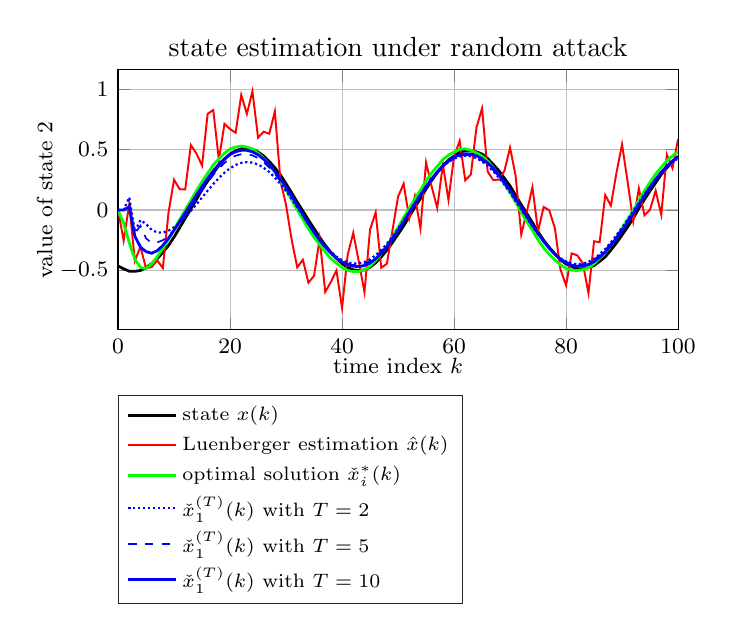
\begin{tikzpicture}
\begin{axis}
	[	width=2.8in,
	height=1.3in,
	at={(0in,1.8in)},
	scale only axis,
	xmin=0,
	xmax=100.0,
%	ymin=-1.5,
%	ymax=0.6,
	title=state estimation under random attack,
	xlabel={\footnotesize time index $k$},
	ylabel={\footnotesize value of state 2},
	x label style={at={(axis description cs:0.5,-0.07)},anchor=north},
	y label style={at={(axis description cs:-0.1,.5)},anchor=south},
	title style={at={(axis description cs:0.5,1.1)},anchor=north},
	xticklabel style = {font=\footnotesize},
	yticklabel style = {font=\footnotesize},
	axis background/.style={fill=white},
	xmajorgrids,
	ymajorgrids,
	legend style={at={(0,-0.25)}, anchor=north west, legend cell align=left, align=left, legend columns=1, draw=white!15!black, font=\scriptsize }]
	\addplot [color={black}, line width=1pt]
	table[row sep={\\}]
	{ 
 0.0  -0.46239997697065616  \\
1.0  -0.4857835862868441  \\
2.0  -0.5057716298872875  \\
3.0  -0.506806692174304  \\
4.0  -0.4996508797564554  \\
5.0  -0.4760789356329692  \\
6.0  -0.4437143748781079  \\
7.0  -0.4014652613603205  \\
8.0  -0.3512599933763697  \\
9.0  -0.29296454811109246  \\
10.0  -0.22390320273806213  \\
11.0  -0.14615391558074686  \\
12.0  -0.06721593551175988  \\
13.0  0.01014178663051969  \\
14.0  0.08766347854829837  \\
15.0  0.16884293860670846  \\
16.0  0.23992493645445367  \\
17.0  0.306587196980928  \\
18.0  0.3686240757738828  \\
19.0  0.4186792565029994  \\
20.0  0.4639083574296991  \\
21.0  0.4908546481896177  \\
22.0  0.5067020161591207  \\
23.0  0.5124601329067985  \\
24.0  0.5034076920974468  \\
25.0  0.47960721759326436  \\
26.0  0.4475082042808572  \\
27.0  0.4015902114271614  \\
28.0  0.34942024242035696  \\
29.0  0.28973781427154527  \\
30.0  0.217831393668124  \\
31.0  0.14252724415876922  \\
32.0  0.06560699580370238  \\
33.0  -0.007577806120277661  \\
34.0  -0.08307402423938813  \\
35.0  -0.15260120807066124  \\
36.0  -0.22647897355909752  \\
37.0  -0.2914897356776189  \\
38.0  -0.3492497830786184  \\
39.0  -0.39930630864255356  \\
40.0  -0.44183183353341865  \\
41.0  -0.475553231883039  \\
42.0  -0.494116189693364  \\
43.0  -0.5012244898714212  \\
44.0  -0.49456723643394807  \\
45.0  -0.4730310926734293  \\
46.0  -0.43507193288560964  \\
47.0  -0.3880075833053857  \\
48.0  -0.33249669261066434  \\
49.0  -0.268082816193912  \\
50.0  -0.1999825373934189  \\
51.0  -0.13086151175796829  \\
52.0  -0.05194412439287283  \\
53.0  0.023326594630945434  \\
54.0  0.0951778861185766  \\
55.0  0.17413065230410052  \\
56.0  0.24485993883446155  \\
57.0  0.3090852489644877  \\
58.0  0.36413576384968693  \\
59.0  0.4138779896234608  \\
60.0  0.44596257018349955  \\
61.0  0.47667282781785814  \\
62.0  0.49280294684902515  \\
63.0  0.49020545944897215  \\
64.0  0.48151213240123997  \\
65.0  0.46307897858213765  \\
66.0  0.4259201802648339  \\
67.0  0.37737002765569283  \\
68.0  0.32584361050278754  \\
69.0  0.2627806670102655  \\
70.0  0.19897595261858295  \\
71.0  0.12167566904462916  \\
72.0  0.044014805314766904  \\
73.0  -0.028941923000465948  \\
74.0  -0.1052055308129323  \\
75.0  -0.1804634774136115  \\
76.0  -0.24998765262637945  \\
77.0  -0.3089091546871591  \\
78.0  -0.360605825675834  \\
79.0  -0.4112735945921447  \\
80.0  -0.44589399661114104  \\
81.0  -0.46686753920352575  \\
82.0  -0.48624312844242035  \\
83.0  -0.4877776724506825  \\
84.0  -0.4766967508298243  \\
85.0  -0.459042098566356  \\
86.0  -0.42367955789972156  \\
87.0  -0.3869083504169279  \\
88.0  -0.3315907895374392  \\
89.0  -0.27186240953322943  \\
90.0  -0.20628938309195105  \\
91.0  -0.13891125280105565  \\
92.0  -0.06713817068572484  \\
93.0  0.013788902705529939  \\
94.0  0.08749847410615302  \\
95.0  0.15867823509488008  \\
96.0  0.2258588170095534  \\
97.0  0.2952447320036467  \\
98.0  0.34930192485437317  \\
99.0  0.40127406555368617  \\
100.0  0.4445263647204763  \\
	};\addlegendentry{{ state ${x}(k)$}}
	
	\addplot [color={red}, line width=0.7pt]
	table[row sep={\\}]
	{
	  0.0  0.0  \\
	 1.0  -0.2521632499552783  \\
	 2.0  0.0490449557742349  \\
	 3.0  -0.42025982952833346  \\
	 4.0  -0.30244468509244615  \\
	 5.0  -0.4831470405389082  \\
	 6.0  -0.47101297885298726  \\
	 7.0  -0.4168063273920141  \\
	 8.0  -0.47955258710382476  \\
	 9.0  -0.024441008301794298  \\
	 10.0  0.2504525285178098  \\
	 11.0  0.17269494049894932  \\
	 12.0  0.17081515684152954  \\
	 13.0  0.5377365592639012  \\
	 14.0  0.46729054983110724  \\
	 15.0  0.3678421742524737  \\
	 16.0  0.7961949636263862  \\
	 17.0  0.8269146567410759  \\
	 18.0  0.4153046690171521  \\
	 19.0  0.7127910203509966  \\
	 20.0  0.6701897856024288  \\
	 21.0  0.6386685377329373  \\
	 22.0  0.9523336126104388  \\
	 23.0  0.7951118023495602  \\
	 24.0  0.9814021441938293  \\
	 25.0  0.5989625147319455  \\
	 26.0  0.6482641098524623  \\
	 27.0  0.6311740975931995  \\
	 28.0  0.815710989473519  \\
	 29.0  0.24132826430620297  \\
	 30.0  0.04192042175506906  \\
	 31.0  -0.24621886700210385  \\
	 32.0  -0.47400781217203347  \\
	 33.0  -0.4110279437488494  \\
	 34.0  -0.6010667829213008  \\
	 35.0  -0.5434429261378935  \\
	 36.0  -0.23742823332188395  \\
	 37.0  -0.6773595083541385  \\
	 38.0  -0.5949779038143711  \\
	 39.0  -0.5000043496552459  \\
	 40.0  -0.8105832990596854  \\
	 41.0  -0.37074672447141044  \\
	 42.0  -0.18871532363161223  \\
	 43.0  -0.4281708423002757  \\
	 44.0  -0.6796251860966278  \\
	 45.0  -0.16207959522072624  \\
	 46.0  -0.02002052520264047  \\
	 47.0  -0.4773208196953683  \\
	 48.0  -0.44356481348922994  \\
	 49.0  -0.1691274145513052  \\
	 50.0  0.11060498949018317  \\
	 51.0  0.21782548303631988  \\
	 52.0  -0.07067332562998155  \\
	 53.0  0.11518992922233394  \\
	 54.0  -0.15195374826862884  \\
	 55.0  0.39469301910945137  \\
	 56.0  0.19395546002146488  \\
	 57.0  0.017171685614179852  \\
	 58.0  0.3768523133298903  \\
	 59.0  0.08440299650531219  \\
	 60.0  0.44221850514549077  \\
	 61.0  0.5716679213502318  \\
	 62.0  0.24562317640670184  \\
	 63.0  0.294275339957324  \\
	 64.0  0.6818867227408865  \\
	 65.0  0.8397446876944941  \\
	 66.0  0.3184685156453132  \\
	 67.0  0.24771075403608056  \\
	 68.0  0.2521387510934531  \\
	 69.0  0.325120915098848  \\
	 70.0  0.5163612745169686  \\
	 71.0  0.28155416041218384  \\
	 72.0  -0.20223739290735065  \\
	 73.0  -0.011519540085583396  \\
	 74.0  0.18798249688926813  \\
	 75.0  -0.17650513523521155  \\
	 76.0  0.026103785406936017  \\
	 77.0  -0.002076301197478092  \\
	 78.0  -0.14880109224320553  \\
	 79.0  -0.49098125172595  \\
	 80.0  -0.6230476419775204  \\
	 81.0  -0.3581107551703351  \\
	 82.0  -0.3746449020204773  \\
	 83.0  -0.4409598142237767  \\
	 84.0  -0.6874349961911861  \\
	 85.0  -0.2581811853417604  \\
	 86.0  -0.2658000871024847  \\
	 87.0  0.12390525579088973  \\
	 88.0  0.036942343618494994  \\
	 89.0  0.3085368853671271  \\
	 90.0  0.543097900932849  \\
	 91.0  0.2314710160200163  \\
	 92.0  -0.09361407263003521  \\
	 93.0  0.17862089196297692  \\
	 94.0  -0.04266777018001397  \\
	 95.0  0.0037565567325872073  \\
	 96.0  0.16082921674291834  \\
	 97.0  -0.039570569737285746  \\
	 98.0  0.45829961316133694  \\
	 99.0  0.34562732368146176  \\
	 100.0  0.5849192718681121  \\
	};\addlegendentry{{ Luenberger estimation $\hat{x}(k)$}}
	
	\addplot [color={green}, line width=1pt]
	table[row sep={\\}]
	{
	  \\
	0.0  0.0  \\
	1.0  -0.10962823953510012  \\
	2.0  -0.27092427627014565  \\
	3.0  -0.40788351211535295  \\
	4.0  -0.4749119925188759  \\
	5.0  -0.48394479998898826  \\
	6.0  -0.44611093687451087  \\
	7.0  -0.38571729955404244  \\
	8.0  -0.3171480919755288  \\
	9.0  -0.2402491250959383  \\
	10.0  -0.1622759168398193  \\
	11.0  -0.07937412200359815  \\
	12.0  1.6839783762003227e-5  \\
	13.0  0.07977270203619355  \\
	14.0  0.16016993026864157  \\
	15.0  0.23489117186917205  \\
	16.0  0.3049525984186638  \\
	17.0  0.3729967060414882  \\
	18.0  0.42357887979738557  \\
	19.0  0.46977713112807024  \\
	20.0  0.5058641636613016  \\
	21.0  0.5209385780037402  \\
	22.0  0.5292512817266898  \\
	23.0  0.521060950790243  \\
	24.0  0.5057604786323736  \\
	25.0  0.469780572980738  \\
	26.0  0.4275253722992635  \\
	27.0  0.37511455440039576  \\
	28.0  0.31302028770694645  \\
	29.0  0.24295838794876726  \\
	30.0  0.1668927729129212  \\
	31.0  0.0862274993090985  \\
	32.0  0.0030460959033294425  \\
	33.0  -0.07591713503352727  \\
	34.0  -0.15551397334527445  \\
	35.0  -0.22672433818535456  \\
	36.0  -0.28618417169325483  \\
	37.0  -0.34671462908976214  \\
	38.0  -0.40164990854265786  \\
	39.0  -0.4388312557669461  \\
	40.0  -0.47526677228759007  \\
	41.0  -0.49925114079335725  \\
	42.0  -0.5089865499145906  \\
	43.0  -0.5072141385378998  \\
	44.0  -0.4940831884672139  \\
	45.0  -0.4638094326926732  \\
	46.0  -0.4164189924963546  \\
	47.0  -0.3590279661891278  \\
	48.0  -0.29548649057941795  \\
	49.0  -0.22275397889690096  \\
	50.0  -0.14407948114801536  \\
	51.0  -0.06165362102332832  \\
	52.0  0.013500430463572115  \\
	53.0  0.09270823872906041  \\
	54.0  0.16445585990411854  \\
	55.0  0.24017414752434071  \\
	56.0  0.3074159920111166  \\
	57.0  0.3622646672588471  \\
	58.0  0.4170856717376843  \\
	59.0  0.4540774301197123  \\
	60.0  0.48050835447745377  \\
	61.0  0.502482507654768  \\
	62.0  0.5061766602263912  \\
	63.0  0.49442479485987967  \\
	64.0  0.47317688379017114  \\
	65.0  0.44651433868034973  \\
	66.0  0.4046349210360333  \\
	67.0  0.3509453031162444  \\
	68.0  0.2863897680750859  \\
	69.0  0.21757922644056976  \\
	70.0  0.1435599231428059  \\
	71.0  0.06540979055283704  \\
	72.0  -0.019601112918802403  \\
	73.0  -0.09614681788263547  \\
	74.0  -0.16877969635326262  \\
	75.0  -0.24569494693724594  \\
	76.0  -0.3116485219765194  \\
	77.0  -0.3673742260768662  \\
	78.0  -0.4132203847043256  \\
	79.0  -0.45147826468860974  \\
	80.0  -0.48289662778263903  \\
	81.0  -0.4959802858050313  \\
	82.0  -0.5004784475859605  \\
	83.0  -0.49232003071742814  \\
	84.0  -0.4775831413827613  \\
	85.0  -0.44414848880732943  \\
	86.0  -0.39962867133587743  \\
	87.0  -0.35093490547662376  \\
	88.0  -0.2924074538074832  \\
	89.0  -0.22410144241130928  \\
	90.0  -0.15046594321967657  \\
	91.0  -0.07699466327827507  \\
	92.0  -0.002866851223090612  \\
	93.0  0.08174991348038603  \\
	94.0  0.1592332799256646  \\
	95.0  0.23035867803160254  \\
	96.0  0.29833146565601815  \\
	97.0  0.3543303389281201  \\
	98.0  0.4087813581187724  \\
	99.0  0.4483047340393276  \\
	100.0  0.483135988865348  \\
	};\addlegendentry{{ optimal solution $\check{x}_i^*(k)$}}
	
	
	\addplot[densely dotted, color={blue}, line width=0.8pt]
	table[row sep={\\}]
	{
		 0.0  0.0  \\
		1.0  0.0  \\
		2.0  0.10525151739465989  \\
		3.0  -0.17850367641573497  \\
		4.0  -0.08310073236487875  \\
		5.0  -0.11571576907783326  \\
		6.0  -0.16282957889015015  \\
		7.0  -0.18561111630427482  \\
		8.0  -0.18658440514345373  \\
		9.0  -0.17098398386601676  \\
		10.0  -0.1418762960292963  \\
		11.0  -0.10279413596303578  \\
		12.0  -0.05697802265866367  \\
		13.0  -0.006415778321040844  \\
		14.0  0.047572313940785184  \\
		15.0  0.10367507585579303  \\
		16.0  0.15995775987947602  \\
		17.0  0.21439913363608448  \\
		18.0  0.26475880808864594  \\
		19.0  0.3089738975818153  \\
		20.0  0.3454688122174652  \\
		21.0  0.3730259471837132  \\
		22.0  0.3903284740285396  \\
		23.0  0.39669714097563025  \\
		24.0  0.39224809861586496  \\
		25.0  0.3767768652697106  \\
		26.0  0.3504045539962246  \\
		27.0  0.31410146022249036  \\
		28.0  0.2687712062138846  \\
		29.0  0.21551808170198997  \\
		30.0  0.15573396818848234  \\
		31.0  0.09119923551842993  \\
		32.0  0.023403648384358003  \\
		33.0  -0.045930774631295745  \\
		34.0  -0.11489206931336673  \\
		35.0  -0.18137268573870918  \\
		36.0  -0.24288187387488405  \\
		37.0  -0.2977260193847972  \\
		38.0  -0.3451762369593187  \\
		39.0  -0.38446604094195114  \\
		40.0  -0.41421945250933495  \\
		41.0  -0.433561518598786  \\
		42.0  -0.44256924180346774  \\
		43.0  -0.44137538323473596  \\
		44.0  -0.42974464265057555  \\
		45.0  -0.4073042284374711  \\
		46.0  -0.37417623888526935  \\
		47.0  -0.33085685231623546  \\
		48.0  -0.27852621124173427  \\
		49.0  -0.21870499322126685  \\
		50.0  -0.15318497841225392  \\
		51.0  -0.08364299548353292  \\
		52.0  -0.011983125669814451  \\
		53.0  0.059596342897499745  \\
		54.0  0.12931750678306228  \\
		55.0  0.19552254916667544  \\
		56.0  0.25692575695274766  \\
		57.0  0.31199907011710315  \\
		58.0  0.3592538980016481  \\
		59.0  0.3973856087516068  \\
		60.0  0.42557418591165946  \\
		61.0  0.4431054756812612  \\
		62.0  0.44949503220623566  \\
		63.0  0.44466552063084236  \\
		64.0  0.42885243693251507  \\
		65.0  0.40250591208263764  \\
		66.0  0.36638084075369654  \\
		67.0  0.32146102655381326  \\
		68.0  0.2685983156738868  \\
		69.0  0.20896276671042363  \\
		70.0  0.1439156546058854  \\
		71.0  0.07528607307998156  \\
		72.0  0.004816143792433933  \\
		73.0  -0.0657506370953354  \\
		74.0  -0.13459093031314828  \\
		75.0  -0.20005559348409316  \\
		76.0  -0.260812618593003  \\
		77.0  -0.3151983257209451  \\
		78.0  -0.3615745228558725  \\
		79.0  -0.3987771721297514  \\
		80.0  -0.42597315681043735  \\
		81.0  -0.4425404897354987  \\
		82.0  -0.44838324332205476  \\
		83.0  -0.44362990874774266  \\
		84.0  -0.4282633418030306  \\
		85.0  -0.40228824016483994  \\
		86.0  -0.36632321549907215  \\
		87.0  -0.3210509977675052  \\
		88.0  -0.26813554068899703  \\
		89.0  -0.20904076259519705  \\
		90.0  -0.14512099472373102  \\
		91.0  -0.07772701677922837  \\
		92.0  -0.008373239908885166  \\
		93.0  0.061443127385525015  \\
		94.0  0.13020666155403504  \\
		95.0  0.19636394668077517  \\
		96.0  0.25802354523818327  \\
		97.0  0.3130489918700365  \\
		98.0  0.360101948461772  \\
		99.0  0.39826452210306573  \\
		100.0  0.4268237321093084  \\
	};\addlegendentry{{$\check{x}_1^{(T)}(k)$ with $T=2$}}

	
	\addplot[dashed, color={blue}, line width=0.6pt]
	table[row sep={\\}]
	{
0.0  0.0  \\
1.0  0.0  \\
2.0  0.0633951446645736  \\
3.0  -0.19370727724916492  \\
4.0  -0.1294893340185907  \\
5.0  -0.23443326234247808  \\
6.0  -0.27093301716017454  \\
7.0  -0.2671845659299317  \\
8.0  -0.24961271942028196  \\
9.0  -0.2153138431825204  \\
10.0  -0.16533186657388527  \\
11.0  -0.1063425701632637  \\
12.0  -0.04149602294161509  \\
13.0  0.026599895799888428  \\
14.0  0.0960516663714602  \\
15.0  0.16431494276897468  \\
16.0  0.22979311185095905  \\
17.0  0.29044273379625213  \\
18.0  0.34421828994716286  \\
19.0  0.3895750134352838  \\
20.0  0.42499923955497604  \\
21.0  0.4496978556636867  \\
22.0  0.4620548428087562  \\
23.0  0.4630445157765113  \\
24.0  0.452138579496872  \\
25.0  0.4291846072539273  \\
26.0  0.3953721147992115  \\
27.0  0.35158931470002397  \\
28.0  0.29897345807589254  \\
29.0  0.23871861978636516  \\
30.0  0.17279353317099633  \\
31.0  0.10224988154740293  \\
32.0  0.028990347695756785  \\
33.0  -0.045441317004057194  \\
34.0  -0.11867322528154978  \\
35.0  -0.18799058300902483  \\
36.0  -0.25088037341106906  \\
37.0  -0.30704542567321225  \\
38.0  -0.3557772118749768  \\
39.0  -0.39566499676725614  \\
40.0  -0.42533485049436276  \\
41.0  -0.4449964486114062  \\
42.0  -0.45504182946289556  \\
43.0  -0.45505821815577324  \\
44.0  -0.44387228876978635  \\
45.0  -0.4213446113133172  \\
46.0  -0.3872934453857896  \\
47.0  -0.3429229177656074  \\
48.0  -0.28939076392326807  \\
49.0  -0.2278917243664729  \\
50.0  -0.16040871641383125  \\
51.0  -0.08884023942875648  \\
52.0  -0.015684155980826356  \\
53.0  0.05708360204535184  \\
54.0  0.12748844740540094  \\
55.0  0.19455952381344996  \\
56.0  0.2568554073350177  \\
57.0  0.312710529842206  \\
58.0  0.3605726051266378  \\
59.0  0.3994904873048468  \\
60.0  0.42848958577893487  \\
61.0  0.44650716394841006  \\
62.0  0.453608485029183  \\
63.0  0.44955428178746965  \\
64.0  0.4344784296653921  \\
65.0  0.4088115899324179  \\
66.0  0.3733812159057809  \\
67.0  0.3289922369398081  \\
68.0  0.2766176584262561  \\
69.0  0.21685905708422046  \\
70.0  0.15153427036023043  \\
71.0  0.08274631615521831  \\
72.0  0.011841109545364159  \\
73.0  -0.0595804040997376  \\
74.0  -0.1293728424246961  \\
75.0  -0.19617043315155233  \\
76.0  -0.25825794860326606  \\
77.0  -0.31356436616486155  \\
78.0  -0.36094314629699525  \\
79.0  -0.39921537097177423  \\
80.0  -0.42732719244426964  \\
81.0  -0.44503661184256876  \\
82.0  -0.4525271236245104  \\
83.0  -0.449268724223732  \\
84.0  -0.4346681595056758  \\
85.0  -0.40973313066406836  \\
86.0  -0.3742725140119453  \\
87.0  -0.32953813558753353  \\
88.0  -0.2774356134459092  \\
89.0  -0.2188638163916315  \\
90.0  -0.15526784481085293  \\
91.0  -0.08788187252510653  \\
92.0  -0.017703248252680465  \\
93.0  0.05321362318664985  \\
94.0  0.1234438767970521  \\
95.0  0.1912466753059259  \\
96.0  0.25434003281558104  \\
97.0  0.31051044747575995  \\
98.0  0.3590088586713575  \\
99.0  0.3987267108088798  \\
100.0  0.429053050882728  \\
	};\addlegendentry{{ $\check{x}_1^{(T)}(k)$ with $T=5$}}
	
	\addplot[ color={blue}, line width=1pt]
	table[row sep={\\}]
	{  0.0  0.0  \\
		1.0  0.0  \\
		2.0  0.026850061167594703  \\
		3.0  -0.2159480685159394  \\
		4.0  -0.3069318697631826  \\
		5.0  -0.3437811250576708  \\
		6.0  -0.35704250117396713  \\
		7.0  -0.336522075683166  \\
		8.0  -0.29258768420225806  \\
		9.0  -0.23402924912159243  \\
		10.0  -0.16693734020525713  \\
		11.0  -0.09556986779289085  \\
		12.0  -0.02234157418765549  \\
		13.0  0.05111269168096621  \\
		14.0  0.12435617466668918  \\
		15.0  0.1950270849707357  \\
		16.0  0.2620548337749552  \\
		17.0  0.3241384724060127  \\
		18.0  0.37851327212266384  \\
		19.0  0.4238852722822296  \\
		20.0  0.4591333873893728  \\
		21.0  0.4827224980104697  \\
		22.0  0.49422986523767576  \\
		23.0  0.493760553623463  \\
		24.0  0.48149357352762584  \\
		25.0  0.45662996813380885  \\
		26.0  0.42069913496332373  \\
		27.0  0.37495849445642476  \\
		28.0  0.3204794608862927  \\
		29.0  0.2580915380548589  \\
		30.0  0.18994496722211837  \\
		31.0  0.1167651398934862  \\
		32.0  0.0403052157161025  \\
		33.0  -0.0374342083650587  \\
		34.0  -0.11343955537096737  \\
		35.0  -0.18416745137362836  \\
		36.0  -0.24838203551068935  \\
		37.0  -0.30574131585697734  \\
		38.0  -0.3562927895450132  \\
		39.0  -0.39782694484714753  \\
		40.0  -0.4293739061800997  \\
		41.0  -0.4515227979993461  \\
		42.0  -0.46471872643527323  \\
		43.0  -0.46783613867279344  \\
		44.0  -0.4587003369983739  \\
		45.0  -0.43674097878019097  \\
		46.0  -0.40260362863501564  \\
		47.0  -0.3575530172226822  \\
		48.0  -0.30226818702055697  \\
		49.0  -0.23880133279019217  \\
		50.0  -0.1692160826871424  \\
		51.0  -0.09535817371857773  \\
		52.0  -0.02044473902909205  \\
		53.0  0.05329465447171586  \\
		54.0  0.1249635751414799  \\
		55.0  0.1937550140991437  \\
		56.0  0.2578335962034861  \\
		57.0  0.31591680002828765  \\
		58.0  0.3659712239663742  \\
		59.0  0.40670246563361223  \\
		60.0  0.43727131596323404  \\
		61.0  0.4574236893224943  \\
		62.0  0.46577707882750435  \\
		63.0  0.46314190375602726  \\
		64.0  0.4494371234995296  \\
		65.0  0.4241166366412594  \\
		66.0  0.3892679132805996  \\
		67.0  0.3455396687046905  \\
		68.0  0.29235877283509215  \\
		69.0  0.23134482680577056  \\
		70.0  0.16478881410837226  \\
		71.0  0.09420335354440364  \\
		72.0  0.021332931061470856  \\
		73.0  -0.052735757600920946  \\
		74.0  -0.12537651814965925  \\
		75.0  -0.19466624112491535  \\
		76.0  -0.2593435269637283  \\
		77.0  -0.3172019697494556  \\
		78.0  -0.3667340790331123  \\
		79.0  -0.4067026591152904  \\
		80.0  -0.43663495533566854  \\
		81.0  -0.45673798169533014  \\
		82.0  -0.46612729595509605  \\
		83.0  -0.4641030196749562  \\
		84.0  -0.4506401671606766  \\
		85.0  -0.426270977815842  \\
		86.0  -0.39062419131885817  \\
		87.0  -0.34571433324248424  \\
		88.0  -0.2929539201261029  \\
		89.0  -0.2344760743768291  \\
		90.0  -0.17004655110529837  \\
		91.0  -0.10065578675031982  \\
		92.0  -0.027981992686906695  \\
		93.0  0.04540297432502287  \\
		94.0  0.11819843874975468  \\
		95.0  0.18936707852510765  \\
		96.0  0.2549021309331391  \\
		97.0  0.31281322380302645  \\
		98.0  0.36331892069814087  \\
		99.0  0.4054791439330571  \\
		100.0  0.4375999253274201  \\	
	};\addlegendentry{{ $\check{x}_1^{(T)}(k)$ with $T=10$}}
\end{axis}
	

\

	
\end{tikzpicture}





		}
\end{figure}
    \end{column}
    \begin{column}{0.5\textwidth}
     \begin{figure}[htpb!]\vspace{90pt}
     	\resizebox{0.5\textheight}{0.5\textheight}{	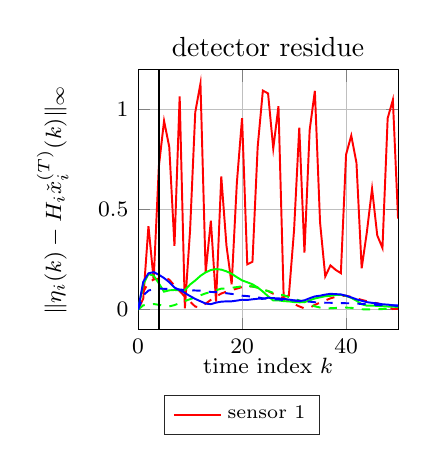
\begin{tikzpicture}
\begin{axis}
	[	width=1.3in,
	height=1.3in,
	at={(0in,0in)},
	scale only axis,
	xmin=0,
	xmax=50.0,
	ymin=-0.1,
	ymax=1.2,
	title=detector residue,
	xlabel={\footnotesize time index $k$},
	ylabel={\footnotesize $\|\eta_i(k)-H_i\check{x}_i^{(T)}(k)\|_\infty$},
	x label style={at={(axis description cs:0.5,-0.07)},anchor=north},
	y label style={at={(axis description cs:-0.23,.5)},anchor=south},
	title style={at={(axis description cs:0.5,1.1)},anchor=north},
	xticklabel style = {font=\footnotesize},
	yticklabel style = {font=\footnotesize},
	axis background/.style={fill=white},
	xmajorgrids,
	ymajorgrids,
	legend style={at={(0.1,-0.25)}, anchor=north west, legend cell align=left, align=left, legend columns=1, draw=white!15!black, font=\scriptsize }]
	\addplot [color={red}, line width=0.7pt]
	table[row sep={\\}]
	{ 
	 0.0  0.0  \\
	1.0  0.055703718502693865  \\
	2.0  0.4180970788138475  \\
	3.0  0.14897997527864734  \\
	4.0  0.7171081733315443  \\
	5.0  0.9443018134309288  \\
	6.0  0.8136486439444562  \\
	7.0  0.31910174637058025  \\
	8.0  1.066818961304309  \\
	9.0  0.007234503503052705  \\
	10.0  0.396599683002509  \\
	11.0  0.9874106594623004  \\
	12.0  1.1310552043411581  \\
	13.0  0.18688772994425282  \\
	14.0  0.4450075263398106  \\
	15.0  0.04083383160467379  \\
	16.0  0.666520216424022  \\
	17.0  0.3204826944703334  \\
	18.0  0.12672505248023802  \\
	19.0  0.6350755029781767  \\
	20.0  0.9582285367033904  \\
	21.0  0.2268507187018777  \\
	22.0  0.23986319971612394  \\
	23.0  0.8136152412551033  \\
	24.0  1.095704536484537  \\
	25.0  1.0815500214951306  \\
	26.0  0.8061482901812206  \\
	27.0  1.0172638329110286  \\
	28.0  0.0649076049358692  \\
	29.0  0.07037862364806176  \\
	30.0  0.39801328956611154  \\
	31.0  0.9105445611043166  \\
	32.0  0.28630643376637727  \\
	33.0  0.8982584649512828  \\
	34.0  1.09435026495013  \\
	35.0  0.4362710974489632  \\
	36.0  0.1666040990618876  \\
	37.0  0.22159655662318167  \\
	38.0  0.19921495650230917  \\
	39.0  0.18287312186782184  \\
	40.0  0.7756513564374694  \\
	41.0  0.8705035602926228  \\
	42.0  0.7344724663851521  \\
	43.0  0.206884710064011  \\
	44.0  0.3880311813727284  \\
	45.0  0.6049768010165284  \\
	46.0  0.3714085329914261  \\
	47.0  0.3088600190954512  \\
	48.0  0.9573447987044231  \\
	49.0  1.049231311013787  \\
	50.0  0.45629644273605485  \\
	51.0  0.8728214426562164  \\
	52.0  0.5688235291306311  \\
	53.0  0.38110685154823165  \\
	54.0  0.04545664633379731  \\
	55.0  0.9486373595180255  \\
	56.0  0.8899982260755439  \\
	57.0  0.210677362826193  \\
	58.0  0.2996378685659556  \\
	59.0  0.9443460708846884  \\
	60.0  0.5266997644229532  \\
	61.0  0.9760576999099294  \\
	62.0  0.5474724532584581  \\
	63.0  0.5723755917547405  \\
	64.0  0.1934728768926591  \\
	65.0  0.07363668173364342  \\
	66.0  0.5931306681329898  \\
	67.0  0.9013420045086533  \\
	68.0  0.8667483800802688  \\
	69.0  0.23602205955401753  \\
	70.0  0.549753615804772  \\
	71.0  0.9556355372651176  \\
	72.0  0.06825030402073941  \\
	73.0  0.8655986098489687  \\
	74.0  0.8603266473015037  \\
	75.0  0.42171435119419814  \\
	76.0  0.367112479250843  \\
	77.0  0.5212868378483083  \\
	78.0  0.517326790615333  \\
	79.0  0.7591731721353501  \\
	80.0  0.5589151428273964  \\
	81.0  0.6550660073767248  \\
	82.0  0.6303994195869873  \\
	83.0  0.4601431335212836  \\
	84.0  0.9697922038220795  \\
	85.0  1.1143002745494843  \\
	86.0  0.29192771785577765  \\
	87.0  1.1382733780197452  \\
	88.0  0.9113799460224172  \\
	89.0  0.7583647301809008  \\
	90.0  1.0766617250305117  \\
	91.0  0.8534163000074024  \\
	92.0  0.7391473479202919  \\
	93.0  0.7145754459523292  \\
	94.0  0.9015276035264541  \\
	95.0  0.41817031414471245  \\
	96.0  0.5324887225056296  \\
	97.0  0.9578956066281439  \\
	98.0  0.9100240367970955  \\
	99.0  0.49779331396490284  \\
	100.0  0.8627103095984349  \\
	};\addlegendentry{sensor 1}
	
	\addplot [dashed, color={red}, line width=0.7pt]
	table[row sep={\\}]
	{
	  0.0  0.0  \\
	  1.0  0.08916336474540897  \\
	  2.0  0.13631756778231657  \\
	  3.0  0.15119031261085134  \\
	  4.0  0.1555971080030611  \\
	  5.0  0.1637077429496924  \\
	  6.0  0.1502400253322839  \\
	  7.0  0.12072291796598209  \\
	  8.0  0.09278699915693973  \\
	  9.0  0.06566445181529448  \\
	  10.0  0.04104649465663344  \\
	  11.0  0.015562028126300264  \\
	  12.0  0.011848778488169483  \\
	  13.0  0.03053690491178505  \\
	  14.0  0.049188463389405315  \\
	  15.0  0.0656416713550842  \\
	  16.0  0.08101588228958682  \\
	  17.0  0.09039034503408447  \\
	  18.0  0.09797110057026277  \\
	  19.0  0.1055037052906202  \\
	  20.0  0.11319786801637831  \\
	  21.0  0.11697483460769188  \\
	  22.0  0.11628930970406626  \\
	  23.0  0.1107068143148839  \\
	  24.0  0.10099301148026575  \\
	  25.0  0.09276148456170116  \\
	  26.0  0.07964935973388328  \\
	  27.0  0.06993856811474217  \\
	  28.0  0.05844227036961038  \\
	  29.0  0.0441008876605453  \\
	  30.0  0.028267419294033588  \\
	  31.0  0.016641974394255098  \\
	  32.0  0.006642111498960579  \\
	  33.0  0.00928251543256892  \\
	  34.0  0.02437371017725158  \\
	  35.0  0.03553075876808716  \\
	  36.0  0.046117076719435934  \\
	  37.0  0.05686651890547882  \\
	  38.0  0.06433581330238664  \\
	  39.0  0.06916567938816284  \\
	  40.0  0.06992818322407743  \\
	  41.0  0.06376045964392771  \\
	  42.0  0.05748541476604116  \\
	  43.0  0.04905884151364118  \\
	  44.0  0.04262860458565296  \\
	  45.0  0.03684528460177641  \\
	  46.0  0.032311467168610344  \\
	  47.0  0.024267572984379107  \\
	  48.0  0.013693240259834205  \\
	  49.0  0.0034649549350843495  \\
	  50.0  0.004719336199742963  \\
	  51.0  0.007218400899505387  \\
	  52.0  0.011174143406651616  \\
	  53.0  0.021036701907431222  \\
	  54.0  0.031385557239003034  \\
	  55.0  0.03859600081057521  \\
	  56.0  0.03862185867566477  \\
	  57.0  0.035828707021960934  \\
	  58.0  0.03467644533423078  \\
	  59.0  0.031978728718393995  \\
	  60.0  0.02951058295013731  \\
	  61.0  0.028616913137620686  \\
	  62.0  0.03284338805828518  \\
	  63.0  0.033233970907114635  \\
	  64.0  0.03350545578559008  \\
	  65.0  0.03080226533219174  \\
	  66.0  0.02469364325262008  \\
	  67.0  0.022637847176615586  \\
	  68.0  0.022861015171318166  \\
	  69.0  0.019525924805445925  \\
	  70.0  0.011827299015493266  \\
	  71.0  0.0015563742595524274  \\
	  72.0  0.009122414093774085  \\
	  73.0  0.01509447889328902  \\
	  74.0  0.0184939097256933  \\
	  75.0  0.02376782544467139  \\
	  76.0  0.027451594838750537  \\
	  77.0  0.02826407622469808  \\
	  78.0  0.026303374696491105  \\
	  79.0  0.02663894391808544  \\
	  80.0  0.028570220561153825  \\
	  81.0  0.02606241048469346  \\
	  82.0  0.022092696017891933  \\
	  83.0  0.01819485448465674  \\
	  84.0  0.0121627294189936  \\
	  85.0  0.006056432082561569  \\
	  86.0  0.005011172993593327  \\
	  87.0  0.0033161294758542598  \\
	  88.0  0.005665593186226295  \\
	  89.0  0.011389763626641375  \\
	  90.0  0.01767316687745328  \\
	  91.0  0.016362768393673906  \\
	  92.0  0.01652873949814558  \\
	  93.0  0.014607016173261461  \\
	  94.0  0.013263035918573474  \\
	  95.0  0.010552816949487953  \\
	  96.0  0.01150206392512132  \\
	  97.0  0.01596061183459671  \\
	  98.0  0.020714888310142843  \\
	  99.0  0.020080309325898577  \\
	  100.0  0.01897298387357907  \\
	};
	
	\addplot [color={green}, line width=0.7pt]
	table[row sep={\\}]
	{
		  0.0  0.0  \\
		1.0  0.12706529355586121  \\
		2.0  0.1784134659688403  \\
		3.0  0.17040372270925425  \\
		4.0  0.13162073678861091  \\
		5.0  0.09026629465622395  \\
		6.0  0.09704935831011256  \\
		7.0  0.09866710494256026  \\
		8.0  0.09729346203852071  \\
		9.0  0.0978975858026383  \\
		10.0  0.12593283586827578  \\
		11.0  0.14630126107450514  \\
		12.0  0.16938451480156763  \\
		13.0  0.18667815145112354  \\
		14.0  0.19852121015788982  \\
		15.0  0.20301965918330783  \\
		16.0  0.2003850675242784  \\
		17.0  0.19193189751970174  \\
		18.0  0.17969082631699798  \\
		19.0  0.16283320265000295  \\
		20.0  0.1466729807745477  \\
		21.0  0.13734591124611145  \\
		22.0  0.1272266604953648  \\
		23.0  0.11119549431316225  \\
		24.0  0.09081047241453243  \\
		25.0  0.06739146668389781  \\
		26.0  0.0461930136103309  \\
		27.0  0.04667485468032421  \\
		28.0  0.0429257021575174  \\
		29.0  0.041585466670699095  \\
		30.0  0.03829314270202035  \\
		31.0  0.03713416360413236  \\
		32.0  0.0375132036153924  \\
		33.0  0.047216538286191045  \\
		34.0  0.056330256629049946  \\
		35.0  0.061983936534384554  \\
		36.0  0.06749206895929827  \\
		37.0  0.06964817785103172  \\
		38.0  0.07360455723884984  \\
		39.0  0.07435030160554809  \\
		40.0  0.06905545925022813  \\
		41.0  0.05922677640142593  \\
		42.0  0.0452367512038111  \\
		43.0  0.027265335712440414  \\
		44.0  0.02029232581193495  \\
		45.0  0.020835119992356044  \\
		46.0  0.019083063329120825  \\
		47.0  0.017608193423899868  \\
		48.0  0.016031652236110264  \\
		49.0  0.014786215599814467  \\
		50.0  0.01595530342248927  \\
		51.0  0.013677392004468297  \\
		52.0  0.005852646537660211  \\
		53.0  0.006905275322657445  \\
		54.0  0.010730514235582078  \\
		55.0  0.009231356569742222  \\
		56.0  0.008697897340745053  \\
		57.0  0.015323082851100678  \\
		58.0  0.023068571660875392  \\
		59.0  0.027533969527718583  \\
		60.0  0.03225128022716256  \\
		61.0  0.04049051634647596  \\
		62.0  0.041833751802836244  \\
		63.0  0.0361932369464959  \\
		64.0  0.022195623944628123  \\
		65.0  0.009942279029969567  \\
		66.0  0.009460114657943552  \\
		67.0  0.02423284167940773  \\
		68.0  0.04087566774232301  \\
		69.0  0.05517386636059268  \\
		70.0  0.06945457428423432  \\
		71.0  0.07632433499109678  \\
		72.0  0.06984788421760707  \\
		73.0  0.0561260371396366  \\
		74.0  0.047306952752906195  \\
		75.0  0.041323479970253374  \\
		76.0  0.03351395478501584  \\
		77.0  0.026291543680593443  \\
		78.0  0.019007954553957873  \\
		79.0  0.018336642508759382  \\
		80.0  0.01372922059470294  \\
		81.0  0.011624404314505288  \\
		82.0  0.012766586976426797  \\
		83.0  0.01574724507164299  \\
		84.0  0.019198755821012534  \\
		85.0  0.01924531132599347  \\
		86.0  0.014002245273102731  \\
		87.0  0.005953179127438091  \\
		88.0  0.006102455730708611  \\
		89.0  0.012668098755917595  \\
		90.0  0.012923757618408055  \\
		91.0  0.018001925250652584  \\
		92.0  0.02858040003419171  \\
		93.0  0.04761657044545897  \\
		94.0  0.0658846449570073  \\
		95.0  0.0852833435615109  \\
		96.0  0.09978072762449597  \\
		97.0  0.10650699460878515  \\
		98.0  0.10025857561937768  \\
		99.0  0.08980173022172128  \\
		100.0  0.08151237343997914  \\
	};
	
	
	\addplot[dashed, color={green}, line width=0.7pt]
	table[row sep={\\}]
	{
		0.0  0.0  \\
		1.0  0.022134678947545318  \\
		2.0  0.02490753968233859  \\
		3.0  0.028735105808354335  \\
		4.0  0.02428632552457479  \\
		5.0  0.020407899237280966  \\
		6.0  0.01674436380306523  \\
		7.0  0.023058833258503067  \\
		8.0  0.033352390103286375  \\
		9.0  0.04384186664835009  \\
		10.0  0.052642782172944845  \\
		11.0  0.06132748502160412  \\
		12.0  0.07216641152270012  \\
		13.0  0.08188987513924886  \\
		14.0  0.0884277500730726  \\
		15.0  0.09723430863182736  \\
		16.0  0.10537655542801383  \\
		17.0  0.1067385503788062  \\
		18.0  0.11006505003342909  \\
		19.0  0.11300181499493642  \\
		20.0  0.11692148714234067  \\
		21.0  0.119094806709897  \\
		22.0  0.11554535006929931  \\
		23.0  0.11063687180014595  \\
		24.0  0.10004326090428967  \\
		25.0  0.09383064770079  \\
		26.0  0.08421048018977509  \\
		27.0  0.07660514825513724  \\
		28.0  0.07281030736495854  \\
		29.0  0.06317145472773625  \\
		30.0  0.05396296504879389  \\
		31.0  0.0465268178326433  \\
		32.0  0.038045989345838756  \\
		33.0  0.029334858509135683  \\
		34.0  0.016869303301928942  \\
		35.0  0.010968727823065606  \\
		36.0  0.005102055591174548  \\
		37.0  0.007718656362973337  \\
		38.0  0.008801626762403161  \\
		39.0  0.00991105640100935  \\
		40.0  0.010261166633379712  \\
		41.0  0.009602737797480946  \\
		42.0  0.005037914409685235  \\
		43.0  0.002364922963304549  \\
		44.0  0.001774701244240031  \\
		45.0  0.0011307966747065787  \\
		46.0  0.002098754029466958  \\
		47.0  0.003427185439602201  \\
		48.0  0.005079929593935835  \\
		49.0  0.012451413045295213  \\
		50.0  0.0156437165241195  \\
		51.0  0.016920222918038894  \\
		52.0  0.01842077631284851  \\
		53.0  0.02304166313355402  \\
		54.0  0.03046754623578747  \\
		55.0  0.03307370360460063  \\
		56.0  0.033119960240935165  \\
		57.0  0.0313370316204066  \\
		58.0  0.03219349137473623  \\
		59.0  0.03165877641731599  \\
		60.0  0.02966334938613993  \\
		61.0  0.027531784355459638  \\
		62.0  0.027494406137596822  \\
		63.0  0.03034944591169908  \\
		64.0  0.030410372071338176  \\
		65.0  0.027766239124880937  \\
		66.0  0.024373388227055537  \\
		67.0  0.0223633510586618  \\
		68.0  0.02082378222282219  \\
		69.0  0.021871232973706967  \\
		70.0  0.016970539184461814  \\
		71.0  0.010851544655231082  \\
		72.0  0.0025389814681268663  \\
		73.0  0.004147603789066048  \\
		74.0  0.0036393853824267103  \\
		75.0  0.005658790199745932  \\
		76.0  0.008034893917082016  \\
		77.0  0.0064518153336383804  \\
		78.0  0.0038369416698501926  \\
		79.0  0.003325527706868614  \\
		80.0  0.00466941499070872  \\
		81.0  0.006135234272452779  \\
		82.0  0.004375500240127256  \\
		83.0  0.0025190857945714996  \\
		84.0  0.005478952348161099  \\
		85.0  0.0063327782812688735  \\
		86.0  0.004864891150863766  \\
		87.0  0.004074826942168638  \\
		88.0  0.0052479111056399005  \\
		89.0  0.010924684951038773  \\
		90.0  0.013859717591074738  \\
		91.0  0.012530805226766153  \\
		92.0  0.009265107869513109  \\
		93.0  0.0060198478299067215  \\
		94.0  0.003761733619509433  \\
		95.0  0.0036395246809585724  \\
		96.0  0.004411313382141541  \\
		97.0  0.00966942091055445  \\
		98.0  0.01441535915165576  \\
		99.0  0.01388027903302863  \\
		100.0  0.013865493810048146  \\
	}
;
	
	\addplot[ color={blue}, line width=0.7pt]
	table[row sep={\\}]
	{
	0.0  0.0  \\
	1.0  0.13975693722966467  \\
	2.0  0.18209634918821663  \\
	3.0  0.18790705867128885  \\
	4.0  0.17481237983523418  \\
	5.0  0.15824296389006776  \\
	6.0  0.13783229940691907  \\
	7.0  0.11076225970246266  \\
	8.0  0.09862790086801577  \\
	9.0  0.08383318421821934  \\
	10.0  0.06817072366346856  \\
	11.0  0.0539833102847765  \\
	12.0  0.04236281719495519  \\
	13.0  0.03073739293771112  \\
	14.0  0.02773065446029027  \\
	15.0  0.035562106645411595  \\
	16.0  0.040305718451499925  \\
	17.0  0.04175929216641494  \\
	18.0  0.042111091787048485  \\
	19.0  0.04558096434464746  \\
	20.0  0.04984806789637583  \\
	21.0  0.0489924469451766  \\
	22.0  0.052107171722311614  \\
	23.0  0.05484465367492678  \\
	24.0  0.05464616823977114  \\
	25.0  0.06001411016350476  \\
	26.0  0.057839573829159906  \\
	27.0  0.056898116890961456  \\
	28.0  0.05373302251424801  \\
	29.0  0.05077215566000069  \\
	30.0  0.04679583574314488  \\
	31.0  0.043072815226603695  \\
	32.0  0.04699394039053953  \\
	33.0  0.0575071662385814  \\
	34.0  0.0666021281007966  \\
	35.0  0.07016254064562333  \\
	36.0  0.07556113768034195  \\
	37.0  0.07945616993061494  \\
	38.0  0.07799547069940985  \\
	39.0  0.07631383951522586  \\
	40.0  0.0701936070508195  \\
	41.0  0.061607300364090234  \\
	42.0  0.052172043107417965  \\
	43.0  0.04480147639423546  \\
	44.0  0.03790787240587401  \\
	45.0  0.03434288396543306  \\
	46.0  0.031593785264350166  \\
	47.0  0.027208788169318265  \\
	48.0  0.025564039282608794  \\
	49.0  0.022203675329376962  \\
	50.0  0.017749000881034052  \\
	51.0  0.016185365472145642  \\
	52.0  0.013709140687341102  \\
	53.0  0.00954080816480847  \\
	54.0  0.006099515241729886  \\
	55.0  0.00428842397274283  \\
	56.0  0.0003354537495171839  \\
	57.0  0.0047505877190699985  \\
	58.0  0.005503448869438064  \\
	59.0  0.005729171729317681  \\
	60.0  0.011282295066061931  \\
	61.0  0.012557264827418771  \\
	62.0  0.012087290031043349  \\
	63.0  0.014040959865650113  \\
	64.0  0.01680285049182964  \\
	65.0  0.016949343585461324  \\
	66.0  0.01900874770234448  \\
	67.0  0.01790498244585323  \\
	68.0  0.017855800673122257  \\
	69.0  0.020784906530325914  \\
	70.0  0.02051316144487665  \\
	71.0  0.01692631306183888  \\
	72.0  0.01378201581159879  \\
	73.0  0.010657193896662042  \\
	74.0  0.007350390324706094  \\
	75.0  0.009825415349443423  \\
	76.0  0.014147166369199715  \\
	77.0  0.014573954892924346  \\
	78.0  0.012297453619330989  \\
	79.0  0.013206762449714082  \\
	80.0  0.015960058586105164  \\
	81.0  0.015805942524331373  \\
	82.0  0.01239747332979585  \\
	83.0  0.006834239878050763  \\
	84.0  0.0081968227525437  \\
	85.0  0.009097893919508243  \\
	86.0  0.007906637799560717  \\
	87.0  0.00990639794033274  \\
	88.0  0.006810030394655692  \\
	89.0  0.004387685421286702  \\
	90.0  0.003731150506554877  \\
	91.0  0.0030808482891765757  \\
	92.0  0.008529757448375922  \\
	93.0  0.015619616746356273  \\
	94.0  0.022363071270592706  \\
	95.0  0.02905251850445581  \\
	96.0  0.030138309679517736  \\
	97.0  0.02279505635687669  \\
	98.0  0.016486694994417808  \\
	99.0  0.018807202639566187  \\
	100.0  0.020032873711731305  \\
	};
	
	\addplot[dashed, color={blue}, line width=0.7pt]
	table[row sep={\\}]
	{ 0.0  0.0  \\
		1.0  0.07165229144760156  \\
		2.0  0.095813925479952  \\
		3.0  0.1023256637476237  \\
		4.0  0.10563031893770775  \\
		5.0  0.10468963908975576  \\
		6.0  0.10446160197165032  \\
		7.0  0.10442089749273512  \\
		8.0  0.10088431395471532  \\
		9.0  0.09894746886695212  \\
		10.0  0.09705118497517008  \\
		11.0  0.09620506721044883  \\
		12.0  0.09505116560232003  \\
		13.0  0.0925697777259909  \\
		14.0  0.0887767261544819  \\
		15.0  0.08781090433847503  \\
		16.0  0.08636188782048723  \\
		17.0  0.08240046576764827  \\
		18.0  0.07892644560102821  \\
		19.0  0.07688586682188327  \\
		20.0  0.0701205365624427  \\
		21.0  0.06815830250362968  \\
		22.0  0.06464273000752424  \\
		23.0  0.06230757570136204  \\
		24.0  0.05684806732914861  \\
		25.0  0.053686342915214666  \\
		26.0  0.052221785038477755  \\
		27.0  0.051536150830963356  \\
		28.0  0.04831793096503206  \\
		29.0  0.04674439463202919  \\
		30.0  0.046047590811127734  \\
		31.0  0.045023336087639615  \\
		32.0  0.04112133956143267  \\
		33.0  0.04024514424064274  \\
		34.0  0.037400112172631755  \\
		35.0  0.037577663660774224  \\
		36.0  0.03484549392926008  \\
		37.0  0.03482284465841065  \\
		38.0  0.03302981111799566  \\
		39.0  0.03294468153566141  \\
		40.0  0.032496190879249556  \\
		41.0  0.032076192495892844  \\
		42.0  0.030431462076841345  \\
		43.0  0.02907211910040486  \\
		44.0  0.02666286923115674  \\
		45.0  0.026343830178644445  \\
		46.0  0.023647790784734224  \\
		47.0  0.0231106943317098  \\
		48.0  0.022650369488486616  \\
		49.0  0.021974533294613907  \\
		50.0  0.022406932633532814  \\
		51.0  0.02149423305863689  \\
		52.0  0.020580831489993193  \\
		53.0  0.02141308534492732  \\
		54.0  0.018430114080734  \\
		55.0  0.01692361496481512  \\
		56.0  0.016463106044832088  \\
		57.0  0.01771640127000214  \\
		58.0  0.01822617378190476  \\
		59.0  0.016712760909490615  \\
		60.0  0.016166014379651594  \\
		61.0  0.015985146771835976  \\
		62.0  0.014237763883667529  \\
		63.0  0.01511619092446334  \\
		64.0  0.012538162685901993  \\
		65.0  0.010723622980056247  \\
		66.0  0.014037054082830236  \\
		67.0  0.013641591424430333  \\
		68.0  0.010793950215088444  \\
		69.0  0.01281560390234232  \\
		70.0  0.012818707504796356  \\
		71.0  0.011914644171804573  \\
		72.0  0.008096517144096343  \\
		73.0  0.006588074300333938  \\
		74.0  0.007235702814613082  \\
		75.0  0.0071983550774041005  \\
		76.0  0.008140794575167226  \\
		77.0  0.00907095258429072  \\
		78.0  0.010035098876069376  \\
		79.0  0.008900439923288733  \\
		80.0  0.008580495290357315  \\
		81.0  0.008382700214118965  \\
		82.0  0.011540716736604367  \\
		83.0  0.010230336487751318  \\
		84.0  0.01012624896618139  \\
		85.0  0.007770460519704203  \\
		86.0  0.0070772314800280345  \\
		87.0  0.0075700939615351015  \\
		88.0  0.004768594344352756  \\
		89.0  0.006570523327540684  \\
		90.0  0.0036064553029993146  \\
		91.0  0.004883829097193315  \\
		92.0  0.003296614432545586  \\
		93.0  0.0017263392237603092  \\
		94.0  0.0026084829566573875  \\
		95.0  0.0021693232898601644  \\
		96.0  0.003281138957834384  \\
		97.0  0.0010195261307130027  \\
		98.0  0.0006028281237949323  \\
		99.0  0.00044624647922875127  \\
		100.0  0.0037943824009415983  \\
	};

	\addplot[color={black}, line width=0.7pt]
	table[row sep={\\}]
	{
		4 -1\\
		4 2\\
	};

\end{axis}
	


	
\end{tikzpicture}




  }
     \end{figure}
    \end{column}
  \end{columns}

\end{frame}


\begin{frame}{Estimation performance under slope signal attack}
  \begin{columns}
	\begin{column}{0.5\textwidth}
		\begin{figure}[htpb!]
			\resizebox{0.8\textheight}{0.8\textheight}{%
				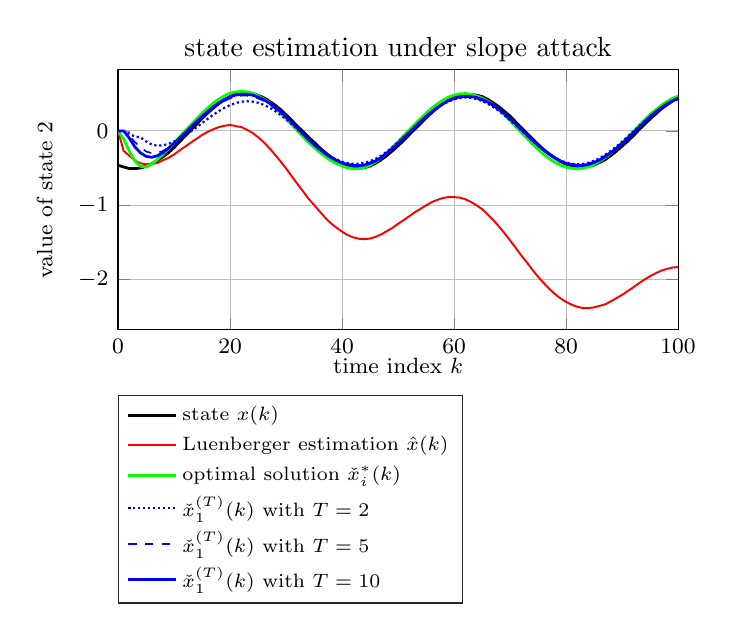
\begin{tikzpicture}





\begin{axis}
	[	width=2.8in,
	height=1.3in,
	at={(0in,0in)},
	scale only axis,
	xmin=0,
	xmax=100.0,
	%	ymin=-1.5,
	%	ymax=0.6,
	title=state estimation under slope attack,
	xlabel={\footnotesize time index $k$},
	ylabel={\footnotesize value of state 2},
	x label style={at={(axis description cs:0.5,-0.07)},anchor=north},
	y label style={at={(axis description cs:-0.1,.5)},anchor=south},
	title style={at={(axis description cs:0.5,1.1)},anchor=north},
	xticklabel style = {font=\footnotesize},
	yticklabel style = {font=\footnotesize},
	axis background/.style={fill=white},
	xmajorgrids,
	ymajorgrids,
	legend style={at={(0,-0.25)}, anchor=north west, legend cell align=left, align=left, legend columns=1, draw=white!15!black, font=\scriptsize }]
	\addplot [color={black}, line width=1pt]
	table[row sep={\\}]
	{ 
	   0.0  -0.46239997697065616  \\
	 1.0  -0.4857835862868441  \\
	 2.0  -0.5057716298872875  \\
	 3.0  -0.506806692174304  \\
	 4.0  -0.4996508797564554  \\
	 5.0  -0.4760789356329692  \\
	 6.0  -0.4437143748781079  \\
	 7.0  -0.4014652613603205  \\
	 8.0  -0.3512599933763697  \\
	 9.0  -0.29296454811109246  \\
	 10.0  -0.22390320273806213  \\
	 11.0  -0.14615391558074686  \\
	 12.0  -0.06721593551175988  \\
	 13.0  0.01014178663051969  \\
	 14.0  0.08766347854829837  \\
	 15.0  0.16884293860670846  \\
	 16.0  0.23992493645445367  \\
	 17.0  0.306587196980928  \\
	 18.0  0.3686240757738828  \\
	 19.0  0.4186792565029994  \\
	 20.0  0.4639083574296991  \\
	 21.0  0.4908546481896177  \\
	 22.0  0.5067020161591207  \\
	 23.0  0.5124601329067985  \\
	 24.0  0.5034076920974468  \\
	 25.0  0.47960721759326436  \\
	 26.0  0.4475082042808572  \\
	 27.0  0.4015902114271614  \\
	 28.0  0.34942024242035696  \\
	 29.0  0.28973781427154527  \\
	 30.0  0.217831393668124  \\
	 31.0  0.14252724415876922  \\
	 32.0  0.06560699580370238  \\
	 33.0  -0.007577806120277661  \\
	 34.0  -0.08307402423938813  \\
	 35.0  -0.15260120807066124  \\
	 36.0  -0.22647897355909752  \\
	 37.0  -0.2914897356776189  \\
	 38.0  -0.3492497830786184  \\
	 39.0  -0.39930630864255356  \\
	 40.0  -0.44183183353341865  \\
	 41.0  -0.475553231883039  \\
	 42.0  -0.494116189693364  \\
	 43.0  -0.5012244898714212  \\
	 44.0  -0.49456723643394807  \\
	 45.0  -0.4730310926734293  \\
	 46.0  -0.43507193288560964  \\
	 47.0  -0.3880075833053857  \\
	 48.0  -0.33249669261066434  \\
	 49.0  -0.268082816193912  \\
	 50.0  -0.1999825373934189  \\
	 51.0  -0.13086151175796829  \\
	 52.0  -0.05194412439287283  \\
	 53.0  0.023326594630945434  \\
	 54.0  0.0951778861185766  \\
	 55.0  0.17413065230410052  \\
	 56.0  0.24485993883446155  \\
	 57.0  0.3090852489644877  \\
	 58.0  0.36413576384968693  \\
	 59.0  0.4138779896234608  \\
	 60.0  0.44596257018349955  \\
	 61.0  0.47667282781785814  \\
	 62.0  0.49280294684902515  \\
	 63.0  0.49020545944897215  \\
	 64.0  0.48151213240123997  \\
	 65.0  0.46307897858213765  \\
	 66.0  0.4259201802648339  \\
	 67.0  0.37737002765569283  \\
	 68.0  0.32584361050278754  \\
	 69.0  0.2627806670102655  \\
	 70.0  0.19897595261858295  \\
	 71.0  0.12167566904462916  \\
	 72.0  0.044014805314766904  \\
	 73.0  -0.028941923000465948  \\
	 74.0  -0.1052055308129323  \\
	 75.0  -0.1804634774136115  \\
	 76.0  -0.24998765262637945  \\
	 77.0  -0.3089091546871591  \\
	 78.0  -0.360605825675834  \\
	 79.0  -0.4112735945921447  \\
	 80.0  -0.44589399661114104  \\
	 81.0  -0.46686753920352575  \\
	 82.0  -0.48624312844242035  \\
	 83.0  -0.4877776724506825  \\
	 84.0  -0.4766967508298243  \\
	 85.0  -0.459042098566356  \\
	 86.0  -0.42367955789972156  \\
	 87.0  -0.3869083504169279  \\
	 88.0  -0.3315907895374392  \\
	 89.0  -0.27186240953322943  \\
	 90.0  -0.20628938309195105  \\
	 91.0  -0.13891125280105565  \\
	 92.0  -0.06713817068572484  \\
	 93.0  0.013788902705529939  \\
	 94.0  0.08749847410615302  \\
	 95.0  0.15867823509488008  \\
	 96.0  0.2258588170095534  \\
	 97.0  0.2952447320036467  \\
	 98.0  0.34930192485437317  \\
	 99.0  0.40127406555368617  \\
	 100.0  0.4445263647204763  \\
	};\addlegendentry{{ state ${x}(k)$}}
	
	\addplot [color={red}, line width=0.7pt]
	table[row sep={\\}]
	{
0.0  0.0  \\
1.0  -0.26908377864009614  \\
2.0  -0.333232733639407  \\
3.0  -0.3996422033962316  \\
4.0  -0.4353167666754484  \\
5.0  -0.44945796611323213  \\
6.0  -0.4426891128213742  \\
7.0  -0.43253658811194406  \\
8.0  -0.3958942554747825  \\
9.0  -0.36317764152297755  \\
10.0  -0.31763795925754823  \\
11.0  -0.2610951462773126  \\
12.0  -0.2105946155888003  \\
13.0  -0.15714529585398349  \\
14.0  -0.1069860740560519  \\
15.0  -0.05487945813536155  \\
16.0  -0.012336489263043177  \\
17.0  0.022052772014015523  \\
18.0  0.051404765099165445  \\
19.0  0.06923528717306686  \\
20.0  0.08088168026612448  \\
21.0  0.06460610365592317  \\
22.0  0.052072369811067984  \\
23.0  0.016188851813580818  \\
24.0  -0.026279532228867947  \\
25.0  -0.08383859299835231  \\
26.0  -0.15058217480404112  \\
27.0  -0.22930629823157722  \\
28.0  -0.3168260035122022  \\
29.0  -0.40806282519173614  \\
30.0  -0.5046106145932111  \\
31.0  -0.6082295440829858  \\
32.0  -0.7105325018774006  \\
33.0  -0.8096024683777407  \\
34.0  -0.9111702905413313  \\
35.0  -0.9955730219638232  \\
36.0  -1.0835890391646266  \\
37.0  -1.1683156994458412  \\
38.0  -1.242722657912896  \\
39.0  -1.3018275215955935  \\
40.0  -1.3560590477015129  \\
41.0  -1.402302707602959  \\
42.0  -1.4332819304167415  \\
43.0  -1.4514533679494397  \\
44.0  -1.4575928969194312  \\
45.0  -1.4482139831439822  \\
46.0  -1.4255819963340788  \\
47.0  -1.3924197372529399  \\
48.0  -1.3485959280600626  \\
49.0  -1.3060086005692408  \\
50.0  -1.2504134548635482  \\
51.0  -1.2019229611980213  \\
52.0  -1.1483286198477485  \\
53.0  -1.0949155701493183  \\
54.0  -1.0496483435835466  \\
55.0  -1.001788791558047  \\
56.0  -0.9592145046969429  \\
57.0  -0.9286104660551815  \\
58.0  -0.9031231103017738  \\
59.0  -0.8905622232394533  \\
60.0  -0.8909427750548427  \\
61.0  -0.8974097237439276  \\
62.0  -0.9191516555731534  \\
63.0  -0.9560160047136214  \\
64.0  -1.0000082618143737  \\
65.0  -1.0525457365152657  \\
66.0  -1.1224070792197378  \\
67.0  -1.198421639879758  \\
68.0  -1.284979675437389  \\
69.0  -1.3762117383246262  \\
70.0  -1.472001888457103  \\
71.0  -1.5736021876048987  \\
72.0  -1.6768374457192659  \\
73.0  -1.7685556599655472  \\
74.0  -1.8698362168895852  \\
75.0  -1.9626143499666333  \\
76.0  -2.0468436835152914  \\
77.0  -2.1264719632031306  \\
78.0  -2.19457909303325  \\
79.0  -2.2543786304738944  \\
80.0  -2.3010617990294677  \\
81.0  -2.338373114699544  \\
82.0  -2.3670353092874947  \\
83.0  -2.3843955363070046  \\
84.0  -2.3837061068933014  \\
85.0  -2.375662496758244  \\
86.0  -2.3550525651245233  \\
87.0  -2.334139094504579  \\
88.0  -2.293244774598523  \\
89.0  -2.2508165697934457  \\
90.0  -2.2076089190398154  \\
91.0  -2.1559496972163297  \\
92.0  -2.1061320249875797  \\
93.0  -2.0506080894049177  \\
94.0  -2.001206628004331  \\
95.0  -1.9552130684924176  \\
96.0  -1.9160896195806811  \\
97.0  -1.8809704956753295  \\
98.0  -1.8579411060386113  \\
99.0  -1.838960829533748  \\
100.0  -1.8330846220672554  \\
	};\addlegendentry{{ Luenberger estimation $\hat{x}(k)$}}
	
	\addplot [color={green}, line width=1pt]
	table[row sep={\\}]
	{
	   0.0  0.0  \\
	1.0  -0.10794958117905912  \\
	2.0  -0.27228049506401963  \\
	3.0  -0.40620330053206816  \\
	4.0  -0.47620382599653405  \\
	5.0  -0.4843924180562346  \\
	6.0  -0.4454376901715596  \\
	7.0  -0.38694455017107815  \\
	8.0  -0.3143324144090187  \\
	9.0  -0.23760177059834073  \\
	10.0  -0.160958864322854  \\
	11.0  -0.07851759286739177  \\
	12.0  0.0027698221125628773  \\
	13.0  0.08221461240815987  \\
	14.0  0.16019087874864915  \\
	15.0  0.23702957323702495  \\
	16.0  0.3091244040912755  \\
	17.0  0.3733303790040993  \\
	18.0  0.4279006568081084  \\
	19.0  0.4726114735301238  \\
	20.0  0.5079593966538962  \\
	21.0  0.5242358588094129  \\
	22.0  0.53199636894794  \\
	23.0  0.5252069780556787  \\
	24.0  0.5058987078199103  \\
	25.0  0.4735538873363581  \\
	26.0  0.4316040762847319  \\
	27.0  0.37832275198731435  \\
	28.0  0.3135071407329328  \\
	29.0  0.24300556547605456  \\
	30.0  0.16695290660127865  \\
	31.0  0.08651189146076686  \\
	32.0  0.004722724431521882  \\
	33.0  -0.07609432417575882  \\
	34.0  -0.1544160502477  \\
	35.0  -0.22272919158293955  \\
	36.0  -0.28574573027566014  \\
	37.0  -0.34542743459277364  \\
	38.0  -0.39838350478575435  \\
	39.0  -0.43887752332363134  \\
	40.0  -0.47178400122477854  \\
	41.0  -0.49582101510366416  \\
	42.0  -0.5093207543945734  \\
	43.0  -0.5077302608791985  \\
	44.0  -0.4922702220745957  \\
	45.0  -0.46063337877789096  \\
	46.0  -0.4160680897380957  \\
	47.0  -0.3603186350028278  \\
	48.0  -0.2927789316407074  \\
	49.0  -0.2199101332251573  \\
	50.0  -0.1415338474687369  \\
	51.0  -0.06352666901192237  \\
	52.0  0.014435774493372047  \\
	53.0  0.09115902298981891  \\
	54.0  0.16541983641699678  \\
	55.0  0.2377414345617255  \\
	56.0  0.30500602979148267  \\
	57.0  0.3636928080205883  \\
	58.0  0.4141782985441153  \\
	59.0  0.4549983078828544  \\
	60.0  0.481127570042233  \\
	61.0  0.49859770523287705  \\
	62.0  0.502825950313663  \\
	63.0  0.49315778219662804  \\
	64.0  0.4718655180469997  \\
	65.0  0.44190939951091757  \\
	66.0  0.39975120604703723  \\
	67.0  0.3479181553517711  \\
	68.0  0.28445683795406485  \\
	69.0  0.2149620945730654  \\
	70.0  0.13940267257350167  \\
	71.0  0.0598372409923574  \\
	72.0  -0.022751337980631052  \\
	73.0  -0.10030809851844014  \\
	74.0  -0.1765695148810341  \\
	75.0  -0.24927259034608884  \\
	76.0  -0.31561295953208746  \\
	77.0  -0.37346650325134645  \\
	78.0  -0.42233822545675087  \\
	79.0  -0.4608109332953346  \\
	80.0  -0.4878785275454189  \\
	81.0  -0.5025058416344732  \\
	82.0  -0.508805263032559  \\
	83.0  -0.5024204085858622  \\
	84.0  -0.483980329714262  \\
	85.0  -0.4521938970039394  \\
	86.0  -0.40800290645908444  \\
	87.0  -0.35946159562919355  \\
	88.0  -0.2996982386365387  \\
	89.0  -0.23322271906636968  \\
	90.0  -0.16212859291052004  \\
	91.0  -0.08815186924005106  \\
	92.0  -0.011461301758024954  \\
	93.0  0.06868614874144759  \\
	94.0  0.14635145949424974  \\
	95.0  0.21963261993232489  \\
	96.0  0.28481973418683765  \\
	97.0  0.3441718982199795  \\
	98.0  0.3951659594615219  \\
	99.0  0.43797279919463133  \\
	100.0  0.4692093821113841  \\
	};\addlegendentry{{ optimal solution $\check{x}_i^*(k)$}}
	
	
	\addplot[densely dotted, color={blue}, line width=0.8pt]
	table[row sep={\\}]
	{     0.0  0.0  \\
		1.0  0.0  \\
		2.0  -0.037137238504787756  \\
		3.0  -0.07625550732298786  \\
		4.0  -0.08569533920817761  \\
		5.0  -0.14028190371707053  \\
		6.0  -0.18223126322373814  \\
		7.0  -0.1990470846018902  \\
		8.0  -0.19461761409051503  \\
		9.0  -0.17457850284297569  \\
		10.0  -0.14340399631270068  \\
		11.0  -0.10414706635467982  \\
		12.0  -0.05849715302348967  \\
		13.0  -0.007523603217366635  \\
		14.0  0.04740501853488495  \\
		15.0  0.10453305333103932  \\
		16.0  0.16159857735453115  \\
		17.0  0.21650683960538897  \\
		18.0  0.2670991831189329  \\
		19.0  0.31141949548070486  \\
		20.0  0.34795696673520715  \\
		21.0  0.37551234112354864  \\
		22.0  0.3927637475358651  \\
		23.0  0.39902584664519636  \\
		24.0  0.39441780176853447  \\
		25.0  0.3787468060581894  \\
		26.0  0.35214924646150536  \\
		27.0  0.31560945389780415  \\
		28.0  0.27004145483988856  \\
		29.0  0.21655637047500145  \\
		30.0  0.15655060616713576  \\
		31.0  0.0918079964681912  \\
		32.0  0.023821320905653656  \\
		33.0  -0.04568483381928774  \\
		34.0  -0.11479665556299527  \\
		35.0  -0.18140567318350626  \\
		36.0  -0.24302113729180347  \\
		37.0  -0.2979501701146483  \\
		38.0  -0.34546513236912496  \\
		39.0  -0.3848011055816947  \\
		40.0  -0.4145838906007278  \\
		41.0  -0.4339404543552234  \\
		42.0  -0.4429498088853362  \\
		43.0  -0.44174676099826765  \\
		44.0  -0.4300980348732955  \\
		45.0  -0.40763278405798736  \\
		46.0  -0.37447492220921724  \\
		47.0  -0.33112227952371265  \\
		48.0  -0.2787564704838578  \\
		49.0  -0.21889945552342804  \\
		50.0  -0.15334410606756543  \\
		51.0  -0.08376815189273894  \\
		52.0  -0.012076390385898667  \\
		53.0  0.05953234922226908  \\
		54.0  0.12927978333297782  \\
		55.0  0.1955078600274339  \\
		56.0  0.25693075838072615  \\
		57.0  0.31202042013452247  \\
		58.0  0.35928834779275776  \\
		59.0  0.3974300779224139  \\
		60.0  0.4256258198085463  \\
		61.0  0.4431616877731783  \\
		62.0  0.4495535305381789  \\
		63.0  0.4447243235425803  \\
		64.0  0.42890987736246683  \\
		65.0  0.402560632640003  \\
		66.0  0.3664317809825727  \\
		67.0  0.32150740328256094  \\
		68.0  0.26863959914728125  \\
		69.0  0.2089986538455676  \\
		70.0  0.14394604026840635  \\
		71.0  0.07531102065438551  \\
		72.0  0.004835856059553126  \\
		73.0  -0.06573584656991782  \\
		74.0  -0.13458066365330867  \\
		75.0  -0.2000493933767678  \\
		76.0  -0.2608099905964836  \\
		77.0  -0.31519875753793497  \\
		78.0  -0.3615775014830572  \\
		79.0  -0.398782198303047  \\
		80.0  -0.42597975665551613  \\
		81.0  -0.44254822347707984  \\
		82.0  -0.44839171135983863  \\
		83.0  -0.4436387565632514  \\
		84.0  -0.4282722626130142  \\
		85.0  -0.402296975592865  \\
		86.0  -0.36633155448099247  \\
		87.0  -0.32105877458348353  \\
		88.0  -0.26814263238135244  \\
		89.0  -0.2090470852003068  \\
		90.0  -0.14512649930690472  \\
		91.0  -0.07773168488552652  \\
		92.0  -0.008377079158310902  \\
		93.0  0.06144008786913971  \\
		94.0  0.13020437523787773  \\
		95.0  0.19636235379456293  \\
		96.0  0.25802257657045913  \\
		97.0  0.31304857241790407  \\
		98.0  0.3601020001577717  \\
		99.0  0.3982649669065971  \\
		100.0  0.4268244936806467  \\
	};\addlegendentry{{$\check{x}_1^{(T)}(k)$ with $T=2$}}
	
	\addplot[dashed, color={blue}, line width=0.6pt]
	table[row sep={\\}]
	{
0.0  0.0  \\
1.0  0.0  \\
2.0  -0.06311454881231054  \\
3.0  -0.15128025857218017  \\
4.0  -0.21728476984305903  \\
5.0  -0.2764007200528965  \\
6.0  -0.2991117878932609  \\
7.0  -0.2967399346316414  \\
8.0  -0.27041507984072244  \\
9.0  -0.22571832566387323  \\
10.0  -0.16886601597816664  \\
11.0  -0.10410576659800763  \\
12.0  -0.03458530569615515  \\
13.0  0.036718015312413754  \\
14.0  0.10844412413064634  \\
15.0  0.17809806991836724  \\
16.0  0.24439805081098276  \\
17.0  0.3054441524556163  \\
18.0  0.3592107531133662  \\
19.0  0.4042406707597953  \\
20.0  0.4391363243018282  \\
21.0  0.4630788427557344  \\
22.0  0.4745620560647869  \\
23.0  0.4747558047624234  \\
24.0  0.46287262420892655  \\
25.0  0.43898344266351014  \\
26.0  0.4042378119969535  \\
27.0  0.3595503016071685  \\
28.0  0.3061625421996262  \\
29.0  0.2451119058629974  \\
30.0  0.17847391129381995  \\
31.0  0.10710145252777158  \\
32.0  0.03299025329039433  \\
33.0  -0.042366885296989405  \\
34.0  -0.11634038241018323  \\
35.0  -0.18607318479312762  \\
36.0  -0.24926713576721204  \\
37.0  -0.30579063299502546  \\
38.0  -0.35488554724602905  \\
39.0  -0.3951508692410486  \\
40.0  -0.4252317417539996  \\
41.0  -0.4455512012487441  \\
42.0  -0.45643190783804116  \\
43.0  -0.45731302823742415  \\
44.0  -0.44678161722389825  \\
45.0  -0.42463232699661974  \\
46.0  -0.3906756022499852  \\
47.0  -0.34633107268018026  \\
48.0  -0.2924814752816437  \\
49.0  -0.2305629932348586  \\
50.0  -0.1626428866189431  \\
51.0  -0.0905652590237694  \\
52.0  -0.017054402223362533  \\
53.0  0.05590347256181376  \\
54.0  0.1264764022009852  \\
55.0  0.1938762957292739  \\
56.0  0.25648046085155524  \\
57.0  0.3127539505261563  \\
58.0  0.3610829074279978  \\
59.0  0.4004225974446874  \\
60.0  0.4297855374653275  \\
61.0  0.4483028235446647  \\
62.0  0.45582414163285123  \\
63.0  0.45213126099415085  \\
64.0  0.4374978596651061  \\
65.0  0.41206775487850633  \\
66.0  0.3768844066898894  \\
67.0  0.33282326799383827  \\
68.0  0.28045876260026614  \\
69.0  0.22051179710418078  \\
70.0  0.1550632742532738  \\
71.0  0.08599686937655292  \\
72.0  0.014698784874364601  \\
73.0  -0.05723318484153499  \\
74.0  -0.12761747571570173  \\
75.0  -0.19499512258774987  \\
76.0  -0.2576554686590848  \\
77.0  -0.3135496816115094  \\
78.0  -0.3614992378635281  \\
79.0  -0.40018853822457545  \\
80.0  -0.42875071407935156  \\
81.0  -0.4470998720008814  \\
82.0  -0.4551672622307117  \\
83.0  -0.45230160116085616  \\
84.0  -0.438094267331355  \\
85.0  -0.41353337247669486  \\
86.0  -0.3781243958960428  \\
87.0  -0.33352783808287584  \\
88.0  -0.28143944763197287  \\
89.0  -0.22296766165813403  \\
90.0  -0.15938295612722234  \\
91.0  -0.09165999804393185  \\
92.0  -0.02096715025297667  \\
93.0  0.05043661298134597  \\
94.0  0.12129163905119136  \\
95.0  0.18989571974092895  \\
96.0  0.2536467398821481  \\
97.0  0.3102746993882863  \\
98.0  0.3593305566885532  \\
99.0  0.3996531735286616  \\
100.0  0.4305141850797336  \\
	};\addlegendentry{{ $\check{x}_1^{(T)}(k)$ with $T=5$}}
	
	\addplot[ color={blue}, line width=1pt]
	table[row sep={\\}]
	{ 0.0  0.0  \\
		1.0  0.0  \\
		2.0  -0.09610232219185627  \\
		3.0  -0.21581820967713397  \\
		4.0  -0.2943966966934804  \\
		5.0  -0.3420385276307325  \\
		6.0  -0.3556337127231199  \\
		7.0  -0.3356409693764213  \\
		8.0  -0.292083980307168  \\
		9.0  -0.23371911703378934  \\
		10.0  -0.16674061420489866  \\
		11.0  -0.09544043284550788  \\
		12.0  -0.02225277090211901  \\
		13.0  0.05117606795211531  \\
		14.0  0.12440303452888324  \\
		15.0  0.1950627751073945  \\
		16.0  0.2620826585730201  \\
		17.0  0.32416055052209136  \\
		18.0  0.37853101596185945  \\
		19.0  0.42389966187308026  \\
		20.0  0.459145130498912  \\
		21.0  0.48273212243178343  \\
		22.0  0.49423777586649353  \\
		23.0  0.4937670684740308  \\
		24.0  0.48149894546621247  \\
		25.0  0.4566344018249092  \\
		26.0  0.42070279589898923  \\
		27.0  0.37496151832543256  \\
		28.0  0.3204819587429515  \\
		29.0  0.2580936022400284  \\
		30.0  0.18994667315982353  \\
		31.0  0.1167665498556755  \\
		32.0  0.04030638125006217  \\
		33.0  -0.03743324458636504  \\
		34.0  -0.11343875854618855  \\
		35.0  -0.18416679247976062  \\
		36.0  -0.24838149055384967  \\
		37.0  -0.3057408653569129  \\
		38.0  -0.3562924169062293  \\
		39.0  -0.39782663667173307  \\
		40.0  -0.42937365138013156  \\
		41.0  -0.45152258733923767  \\
		42.0  -0.4647185525192712  \\
		43.0  -0.46783599492140143  \\
		44.0  -0.4587002180620571  \\
		45.0  -0.43674088079281503  \\
		46.0  -0.40260354785519786  \\
		47.0  -0.35755295023874384  \\
		48.0  -0.3022681316878726  \\
		49.0  -0.23880128730617578  \\
		50.0  -0.16921604518158995  \\
		51.0  -0.09535814279565048  \\
		52.0  -0.02044471335937041  \\
		53.0  0.053294675604658795  \\
		54.0  0.1249635927004234  \\
		55.0  0.19375502881865225  \\
		56.0  0.2578336082985462  \\
		57.0  0.3159168100625645  \\
		58.0  0.3659712323788739  \\
		59.0  0.406702472529685  \\
		60.0  0.43727132171476146  \\
		61.0  0.4574236939365563  \\
		62.0  0.4657770826510255  \\
		63.0  0.4631419068475984  \\
		64.0  0.4494371256802524  \\
		65.0  0.4241166382067672  \\
		66.0  0.38926791489761936  \\
		67.0  0.34553967015263004  \\
		68.0  0.2923587740725472  \\
		69.0  0.23134482786156452  \\
		70.0  0.16478881494892078  \\
		71.0  0.09420335462369281  \\
		72.0  0.02133293198566484  \\
		73.0  -0.052735756500645214  \\
		74.0  -0.12537651717837603  \\
		75.0  -0.19466624029704088  \\
		76.0  -0.25934352619536216  \\
		77.0  -0.3172019691614593  \\
		78.0  -0.3667340786637684  \\
		79.0  -0.4067026589729027  \\
		80.0  -0.43663495544266306  \\
		81.0  -0.4567379822097707  \\
		82.0  -0.4661272967987774  \\
		83.0  -0.46410302064958875  \\
		84.0  -0.4506401680476594  \\
		85.0  -0.42627097922696056  \\
		86.0  -0.390624192748692  \\
		87.0  -0.3457143348909279  \\
		88.0  -0.2929539217702601  \\
		89.0  -0.23447607620420388  \\
		90.0  -0.17004655276273103  \\
		91.0  -0.10065578820977707  \\
		92.0  -0.02798199373076954  \\
		93.0  0.04540297346369325  \\
		94.0  0.11819843810218238  \\
		95.0  0.18936707810187295  \\
		96.0  0.25490213069729467  \\
		97.0  0.3128132236116281  \\
		98.0  0.3633189206865161  \\
		99.0  0.40547914397359286  \\
		100.0  0.4375999254457768  \\
	};\addlegendentry{{ $\check{x}_1^{(T)}(k)$ with $T=10$}}
		
	
\end{axis}

	
\end{tikzpicture}





			}
		\end{figure}
	\end{column}
	\begin{column}{0.5\textwidth}
		\begin{figure}[htpb!]\vspace{90pt}
			\resizebox{0.5\textheight}{0.5\textheight}{	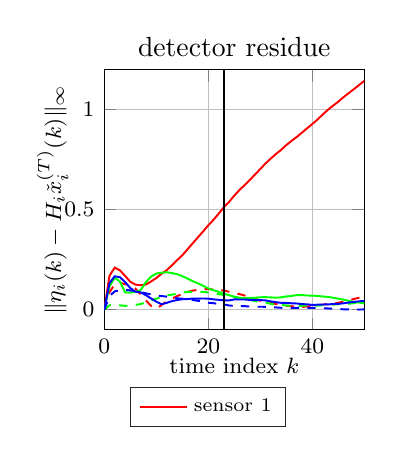
\begin{tikzpicture}





\begin{axis}
	[	width=1.3in,
	height=1.3in,
	at={(1.6in,0in)},
	scale only axis,
	xmin=0,
	xmax=50.0,
	ymin=-0.1,
	ymax=1.2,
	title=detector residue ,
	xlabel={\footnotesize time index $k$},
	ylabel={\footnotesize $\|\eta_i(k)-H_i\check{x}_i^{(T)}(k)\|_\infty$},
	x label style={at={(axis description cs:0.5,-0.07)},anchor=north},
	y label style={at={(axis description cs:-0.1,.5)},anchor=south},
	title style={at={(axis description cs:0.5,1.1)},anchor=north},
	xticklabel style = {font=\footnotesize},
	yticklabel style = {font=\footnotesize},
	axis background/.style={fill=white},
	xmajorgrids,
	ymajorgrids,
	legend style={at={(0.1,-0.22)}, anchor=north west, legend cell align=left, align=left, legend columns=3, draw=white!15!black, font=\scriptsize }]
		\addplot [color={red}, line width=0.7pt]
	table[row sep={\\}]
	{ 
		 0.0  0.0  \\
		1.0  0.1691111855462358  \\
		2.0  0.21046939905252016  \\
		3.0  0.1973144557647789  \\
		4.0  0.16916654977966858  \\
		5.0  0.13981788881481005  \\
		6.0  0.12558057281121876  \\
		7.0  0.12234317984050608  \\
		8.0  0.12556551506920918  \\
		9.0  0.14146894521125447  \\
		10.0  0.15814103114057393  \\
		11.0  0.1800714222783851  \\
		12.0  0.19733991342711804  \\
		13.0  0.22168750363450626  \\
		14.0  0.24742378576476848  \\
		15.0  0.27206525019604  \\
		16.0  0.3016692588679265  \\
		17.0  0.3318916352912695  \\
		18.0  0.36151262390229943  \\
		19.0  0.3910891974766165  \\
		20.0  0.4219015573213933  \\
		21.0  0.4492660814718961  \\
		22.0  0.4802942102741161  \\
		23.0  0.51252848197167  \\
		24.0  0.5391941503451293  \\
		25.0  0.5704149169506718  \\
		26.0  0.5984230286053782  \\
		27.0  0.623443769818855  \\
		28.0  0.6491805163351454  \\
		29.0  0.6762776227149867  \\
		30.0  0.7036073997186283  \\
		31.0  0.7308936234323926  \\
		32.0  0.7551857474022815  \\
		33.0  0.7783184195809967  \\
		34.0  0.7990073696735173  \\
		35.0  0.8230383842019917  \\
		36.0  0.8438434146086775  \\
		37.0  0.8635740127770415  \\
		38.0  0.8850553319560299  \\
		39.0  0.9070788198538784  \\
		40.0  0.9284818857207532  \\
		41.0  0.9508502893624374  \\
		42.0  0.9758740751077862  \\
		43.0  0.9994291163006154  \\
		44.0  1.0205470238946037  \\
		45.0  1.0399948227234874  \\
		46.0  1.0625459275190337  \\
		47.0  1.0826292073917856  \\
		48.0  1.1027280683427736  \\
		49.0  1.1234619367020506  \\
		50.0  1.144241104565793  \\
		51.0  1.1676992023849853  \\
		52.0  1.190398451265985  \\
		53.0  1.21316180327235  \\
		54.0  1.2367931074061989  \\
		55.0  1.2583679301590462  \\
		56.0  1.2823392344598399  \\
		57.0  1.3077518639216885  \\
		58.0  1.3314858303023318  \\
		59.0  1.3543432098189818  \\
		60.0  1.379168904219098  \\
		61.0  1.4043748817439214  \\
		62.0  1.426511386913404  \\
		63.0  1.4532574338350963  \\
		64.0  1.4747254930046374  \\
		65.0  1.4969193646877172  \\
		66.0  1.5204681612945157  \\
		67.0  1.5468983013183277  \\
		68.0  1.5711033764922888  \\
		69.0  1.5920862655846464  \\
		70.0  1.6125366843769235  \\
		71.0  1.6336008728840803  \\
		72.0  1.6572921783112757  \\
		73.0  1.6810569336670391  \\
		74.0  1.7047648077398225  \\
		75.0  1.7249127529445614  \\
		76.0  1.7478559737720618  \\
		77.0  1.7705234497999365  \\
		78.0  1.7979937325480406  \\
		79.0  1.8244213985678246  \\
		80.0  1.8488967403898182  \\
		81.0  1.8691137419378576  \\
		82.0  1.8929429704047571  \\
		83.0  1.9140596105603267  \\
		84.0  1.9392072672207175  \\
		85.0  1.9610987541304625  \\
		86.0  1.984241365994205  \\
		87.0  2.007294289167093  \\
		88.0  2.0295540565209915  \\
		89.0  2.0513067017262117  \\
		90.0  2.072625110988313  \\
		91.0  2.098858620533006  \\
		92.0  2.12155354830093  \\
		93.0  2.1429116210691372  \\
		94.0  2.1652030352153258  \\
		95.0  2.1895566040565564  \\
		96.0  2.214478619738647  \\
		97.0  2.2355539732435443  \\
		98.0  2.256959212545393  \\
		99.0  2.2776898172608786  \\
		100.0  2.3044997562274045  \\
	};\addlegendentry{sensor 1}
	
	\addplot [dashed, color={red}, line width=0.7pt]
	table[row sep={\\}]
	{
		 0.0  0.0  \\
		1.0  0.08655454279558177  \\
		2.0  0.1276578983029523  \\
		3.0  0.13548375809276447  \\
		4.0  0.1274213311749426  \\
		5.0  0.126292381478612  \\
		6.0  0.10582946305487284  \\
		7.0  0.07597981062756289  \\
		8.0  0.04707542988068748  \\
		9.0  0.019002411100958225  \\
		10.0  0.0048040899672308  \\
		11.0  0.023129809706439873  \\
		12.0  0.04206517106480967  \\
		13.0  0.05575952690972808  \\
		14.0  0.06783828141678805  \\
		15.0  0.0788880535248814  \\
		16.0  0.08891149578303453  \\
		17.0  0.09541946970299116  \\
		18.0  0.0998393069662798  \\
		19.0  0.10228988607653229  \\
		20.0  0.10303531339346934  \\
		21.0  0.10104329976572873  \\
		22.0  0.09947047765431964  \\
		23.0  0.09546112725932092  \\
		24.0  0.09013482938408736  \\
		25.0  0.08449023116433498  \\
		26.0  0.07801961826237906  \\
		27.0  0.07104488656936293  \\
		28.0  0.06204805646485154  \\
		29.0  0.05398958125101582  \\
		30.0  0.04527478243486021  \\
		31.0  0.03933620832395305  \\
		32.0  0.034712956445216284  \\
		33.0  0.02876355491609004  \\
		34.0  0.024477952386970037  \\
		35.0  0.020069863061700013  \\
		36.0  0.01736252956908889  \\
		37.0  0.014480460395436365  \\
		38.0  0.013883616530251428  \\
		39.0  0.01577472867927371  \\
		40.0  0.020385770680522386  \\
		41.0  0.02123156800672027  \\
		42.0  0.02575175079959921  \\
		43.0  0.027708316308635905  \\
		44.0  0.029945352516103446  \\
		45.0  0.03499715063316697  \\
		46.0  0.04085345935144949  \\
		47.0  0.04707603916439698  \\
		48.0  0.053735697615608854  \\
		49.0  0.05982013766647343  \\
		50.0  0.06669568784767721  \\
		51.0  0.07450341321350976  \\
		52.0  0.08022280435874492  \\
		53.0  0.08670446950798391  \\
		54.0  0.09296477567441343  \\
		55.0  0.098833465049282  \\
		56.0  0.10194920956295865  \\
		57.0  0.10229271878810806  \\
		58.0  0.10114832533371178  \\
		59.0  0.10003586011692939  \\
		60.0  0.1014579888786539  \\
		61.0  0.10237229917358359  \\
		62.0  0.10301191584428553  \\
		63.0  0.09902568802729037  \\
		64.0  0.09563168512768822  \\
		65.0  0.09165081909965613  \\
		66.0  0.08537873941829648  \\
		67.0  0.0808293165550763  \\
		68.0  0.07701529934014732  \\
		69.0  0.0708587634626745  \\
		70.0  0.06524382333401009  \\
		71.0  0.0604244419982459  \\
		72.0  0.056098676052353656  \\
		73.0  0.0525508777268137  \\
		74.0  0.04910685504470014  \\
		75.0  0.0482068385700926  \\
		76.0  0.04833178696087803  \\
		77.0  0.04769141631704901  \\
		78.0  0.04797430217629972  \\
		79.0  0.047280177867045275  \\
		80.0  0.04833737165103294  \\
		81.0  0.050303088366127735  \\
		82.0  0.051865434803360894  \\
		83.0  0.053038575499753715  \\
		84.0  0.05639262729534439  \\
		85.0  0.0611225495405463  \\
		86.0  0.06678587030464364  \\
		87.0  0.07123286537998891  \\
		88.0  0.07444416540460042  \\
		89.0  0.07906769621874425  \\
		90.0  0.08372350931545731  \\
		91.0  0.08762903661156626  \\
		92.0  0.09494995374959714  \\
		93.0  0.09997675862515827  \\
		94.0  0.10509913831367651  \\
		95.0  0.10825479512865861  \\
		96.0  0.11191574219982318  \\
		97.0  0.11386248402438989  \\
		98.0  0.11550879164761461  \\
		99.0  0.11731976147936042  \\
		100.0  0.11782838951865508  \\
	};
	
	\addplot [color={green}, line width=0.7pt]
	table[row sep={\\}]
	{
	  0.0  0.0  \\
	1.0  0.11606498590416617  \\
	2.0  0.16020746800829477  \\
	3.0  0.14128731932371988  \\
	4.0  0.08718024818529146  \\
	5.0  0.08510443243593685  \\
	6.0  0.08920280968928604  \\
	7.0  0.09800204534478799  \\
	8.0  0.13794872683680273  \\
	9.0  0.1658069821951389  \\
	10.0  0.18083165511760171  \\
	11.0  0.18523840050479792  \\
	12.0  0.18718568783136885  \\
	13.0  0.1834607946555268  \\
	14.0  0.17741470553370486  \\
	15.0  0.1680493140314715  \\
	16.0  0.15578036675803594  \\
	17.0  0.14292086802272247  \\
	18.0  0.13206344270038406  \\
	19.0  0.1196348548488638  \\
	20.0  0.10680632392575906  \\
	21.0  0.09755253103069353  \\
	22.0  0.0892063568154984  \\
	23.0  0.07964255269391193  \\
	24.0  0.07246840939504798  \\
	25.0  0.06530569362833868  \\
	26.0  0.05988374532282956  \\
	27.0  0.05731576295440716  \\
	28.0  0.05848196268053801  \\
	29.0  0.05942354136749334  \\
	30.0  0.06242966929158256  \\
	31.0  0.06277263043589831  \\
	32.0  0.062045746400383295  \\
	33.0  0.0598568542418636  \\
	34.0  0.06190575367537543  \\
	35.0  0.06644669796401675  \\
	36.0  0.06875322037613607  \\
	37.0  0.07333631482326847  \\
	38.0  0.0732170066953921  \\
	39.0  0.07122007293772548  \\
	40.0  0.07040838763507745  \\
	41.0  0.06897498944711816  \\
	42.0  0.06628900568997947  \\
	43.0  0.06388683261641825  \\
	44.0  0.060084871336907625  \\
	45.0  0.05531773294185785  \\
	46.0  0.050264311484819024  \\
	47.0  0.04472479855802647  \\
	48.0  0.03915741806886536  \\
	49.0  0.035496082254370565  \\
	50.0  0.032220285136739885  \\
	51.0  0.031392593131627816  \\
	52.0  0.031878148202373724  \\
	53.0  0.03447922056028119  \\
	54.0  0.03556337885649949  \\
	55.0  0.03689953356479731  \\
	56.0  0.03789192583556057  \\
	57.0  0.0398363502748157  \\
	58.0  0.041343926749395916  \\
	59.0  0.04250029506072142  \\
	60.0  0.04351716831613227  \\
	61.0  0.046507675192376516  \\
	62.0  0.04596247728224814  \\
	63.0  0.046528689844566956  \\
	64.0  0.047371230872744585  \\
	65.0  0.05393391471041532  \\
	66.0  0.061211867063023645  \\
	67.0  0.07010470568341655  \\
	68.0  0.07996156952442224  \\
	69.0  0.0863306005970636  \\
	70.0  0.09524547958222482  \\
	71.0  0.10419888907820554  \\
	72.0  0.1085018792933542  \\
	73.0  0.10934439768856025  \\
	74.0  0.11060701711829624  \\
	75.0  0.11210001015278898  \\
	76.0  0.11295437159337607  \\
	77.0  0.11211210149497386  \\
	78.0  0.10572158824208794  \\
	79.0  0.10006733021774966  \\
	80.0  0.09124109975557088  \\
	81.0  0.08579159522589053  \\
	82.0  0.08135062051348557  \\
	83.0  0.07625649283445779  \\
	84.0  0.07055001885075067  \\
	85.0  0.0607882779173958  \\
	86.0  0.05061083466470398  \\
	87.0  0.04539560104348267  \\
	88.0  0.04056206946771285  \\
	89.0  0.04268603886949479  \\
	90.0  0.04261973429595402  \\
	91.0  0.04592649536981938  \\
	92.0  0.04625452660065166  \\
	93.0  0.049665308784475434  \\
	94.0  0.04931897375334836  \\
	95.0  0.050747553628261985  \\
	96.0  0.05070210671206722  \\
	97.0  0.05263870482961326  \\
	98.0  0.05261235265082004  \\
	99.0  0.054105124539439685  \\
	100.0  0.05441105403198965  \\
	};
	
	
	\addplot[dashed, color={green}, line width=0.7pt]
	table[row sep={\\}]
	{
	0.0  0.0  \\
	1.0  0.02241940536425412  \\
	2.0  0.024444021367625166  \\
	3.0  0.02202522691811712  \\
	4.0  0.01912419321266849  \\
	5.0  0.021515395125992272  \\
	6.0  0.023994078479232305  \\
	7.0  0.028332000728595  \\
	8.0  0.03733150349686444  \\
	9.0  0.047632352191374155  \\
	10.0  0.055003191808325316  \\
	11.0  0.06359101154202082  \\
	12.0  0.07141197702099593  \\
	13.0  0.07538836586394333  \\
	14.0  0.07974502334853534  \\
	15.0  0.0851809195306501  \\
	16.0  0.0896512803072308  \\
	17.0  0.0889334039543183  \\
	18.0  0.0899032077582414  \\
	19.0  0.0887478259629453  \\
	20.0  0.08658766507245297  \\
	21.0  0.08300936907930898  \\
	22.0  0.07764240359918098  \\
	23.0  0.0736565787012336  \\
	24.0  0.06689754156286101  \\
	25.0  0.06312471270720435  \\
	26.0  0.05820451172535121  \\
	27.0  0.052476721303662724  \\
	28.0  0.04932429400233743  \\
	29.0  0.042845411393136176  \\
	30.0  0.03817594537188043  \\
	31.0  0.03477178433626142  \\
	32.0  0.02970488372965653  \\
	33.0  0.024368606990780944  \\
	34.0  0.024013055140635384  \\
	35.0  0.021368402979710488  \\
	36.0  0.018786766415355018  \\
	37.0  0.01793223703481693  \\
	38.0  0.019670879956249283  \\
	39.0  0.020285750520185733  \\
	40.0  0.02083506122562287  \\
	41.0  0.020580564917959825  \\
	42.0  0.02319353335013835  \\
	43.0  0.024422763633964704  \\
	44.0  0.025140468179561674  \\
	45.0  0.02744163479402776  \\
	46.0  0.02896211749188455  \\
	47.0  0.029185358466256226  \\
	48.0  0.03330148792526661  \\
	49.0  0.03828692942420449  \\
	50.0  0.041988597727213264  \\
	51.0  0.04531569681763119  \\
	52.0  0.0465497407751718  \\
	53.0  0.05086507402517425  \\
	54.0  0.054108859205713344  \\
	55.0  0.054206074468501786  \\
	56.0  0.055077620964635754  \\
	57.0  0.05611321049796161  \\
	58.0  0.05833278851953119  \\
	59.0  0.05713331633231861  \\
	60.0  0.05607341115344902  \\
	61.0  0.05473340006279018  \\
	62.0  0.05528669554329835  \\
	63.0  0.051494817607691395  \\
	64.0  0.048929149043289655  \\
	65.0  0.04682301107559195  \\
	66.0  0.0450383582588994  \\
	67.0  0.04325685052246939  \\
	68.0  0.03978814614189778  \\
	69.0  0.04024039242330646  \\
	70.0  0.037478115074801366  \\
	71.0  0.03266098420151517  \\
	72.0  0.03116974579047073  \\
	73.0  0.03102196628576124  \\
	74.0  0.03004210750903677  \\
	75.0  0.030389419059805592  \\
	76.0  0.032620032025534804  \\
	77.0  0.0331837859726159  \\
	78.0  0.03270924993507627  \\
	79.0  0.03301543460116712  \\
	80.0  0.03264595055898825  \\
	81.0  0.03474429112373168  \\
	82.0  0.03684049606821641  \\
	83.0  0.03618033637945202  \\
	84.0  0.03779858641879245  \\
	85.0  0.0380748524197777  \\
	86.0  0.04042783999229907  \\
	87.0  0.04315508813432041  \\
	88.0  0.04355391458862295  \\
	89.0  0.045806087229126574  \\
	90.0  0.046067293058178894  \\
	91.0  0.047254252377637584  \\
	92.0  0.048429116377244244  \\
	93.0  0.05170204335631551  \\
	94.0  0.053450515438259336  \\
	95.0  0.05471322407426506  \\
	96.0  0.057340097466730605  \\
	97.0  0.05760081692853533  \\
	98.0  0.057555177895217996  \\
	99.0  0.05923669093615205  \\
	100.0  0.057167759150816955  \\
	}
	;
	
	\addplot[ color={blue}, line width=0.7pt]
	table[row sep={\\}]
	{
	        0.0  0.0  \\
	1.0  0.13252410503760584  \\
	2.0  0.16710043878875847  \\
	3.0  0.16248840741421805  \\
	4.0  0.13884192530728268  \\
	5.0  0.10856624219197177  \\
	6.0  0.08998751129772037  \\
	7.0  0.08689657406684503  \\
	8.0  0.07280359260195121  \\
	9.0  0.056287344346135755  \\
	10.0  0.0404738824500432  \\
	11.0  0.027406705928411088  \\
	12.0  0.03436902593589766  \\
	13.0  0.04279203517153435  \\
	14.0  0.04853394741954167  \\
	15.0  0.052212132686765354  \\
	16.0  0.05358580551444553  \\
	17.0  0.05545580004744961  \\
	18.0  0.05560971236477832  \\
	19.0  0.05620962618164342  \\
	20.0  0.05538844633706438  \\
	21.0  0.05189500711982668  \\
	22.0  0.04960291429860013  \\
	23.0  0.04698197162613002  \\
	24.0  0.046217906770478254  \\
	25.0  0.05155399024529726  \\
	26.0  0.05109841656792137  \\
	27.0  0.05119125282636918  \\
	28.0  0.04913354286118635  \\
	29.0  0.04874579384936615  \\
	30.0  0.048076348430893596  \\
	31.0  0.04670775963471971  \\
	32.0  0.04175364499251355  \\
	33.0  0.037815467592036786  \\
	34.0  0.03444083126353453  \\
	35.0  0.03399701936630712  \\
	36.0  0.03219329119506337  \\
	37.0  0.03122478267858833  \\
	38.0  0.028078595606083036  \\
	39.0  0.027015351893857648  \\
	40.0  0.023897512336819304  \\
	41.0  0.025152261098266904  \\
	42.0  0.026198362527092567  \\
	43.0  0.026464532814185815  \\
	44.0  0.02853403569112481  \\
	45.0  0.02926408426182628  \\
	46.0  0.032119738462097175  \\
	47.0  0.035953211953978575  \\
	48.0  0.038942769353844886  \\
	49.0  0.042133536759587795  \\
	50.0  0.043636992595134816  \\
	51.0  0.04698806398999063  \\
	52.0  0.048920959668335026  \\
	53.0  0.05066878873434308  \\
	54.0  0.05290915502838488  \\
	55.0  0.05477861338429185  \\
	56.0  0.05603011543000738  \\
	57.0  0.05628341001905132  \\
	58.0  0.05673732692946619  \\
	59.0  0.05841620159027134  \\
	60.0  0.05841807561910234  \\
	61.0  0.058514400062725624  \\
	62.0  0.05833552842832216  \\
	63.0  0.05873820194777231  \\
	64.0  0.058344551959497656  \\
	65.0  0.05887665598426829  \\
	66.0  0.059077117029085094  \\
	67.0  0.05841500630625171  \\
	68.0  0.05894109073211369  \\
	69.0  0.05707242739185095  \\
	70.0  0.05660087546295961  \\
	71.0  0.0570343160286608  \\
	72.0  0.05632389305401933  \\
	73.0  0.0561077864963227  \\
	74.0  0.05701831788305739  \\
	75.0  0.05675148255009416  \\
	76.0  0.05579097336440042  \\
	77.0  0.05330347833639787  \\
	78.0  0.05146488230686591  \\
	79.0  0.04916881569254761  \\
	80.0  0.04913509319757092  \\
	81.0  0.046529964906926735  \\
	82.0  0.045313177517296355  \\
	83.0  0.046626648225997075  \\
	84.0  0.04784021405975308  \\
	85.0  0.04910517866567707  \\
	86.0  0.04855088203089572  \\
	87.0  0.048567700111323775  \\
	88.0  0.05029176529960934  \\
	89.0  0.05135433934755815  \\
	90.0  0.052277260691964665  \\
	91.0  0.05442021337117864  \\
	92.0  0.058377371978968376  \\
	93.0  0.05991773887489839  \\
	94.0  0.060831675789397084  \\
	95.0  0.060603531504495226  \\
	96.0  0.06094201205059152  \\
	97.0  0.06257471007251413  \\
	98.0  0.06382211822906639  \\
	99.0  0.06432098390568541  \\
	100.0  0.06331266762893077  \\
	};
	
	\addplot[dashed, color={blue}, line width=0.7pt]
	table[row sep={\\}]
	{  0.0  0.0  \\
		1.0  0.06849901899515243  \\
		2.0  0.09146596263146133  \\
		3.0  0.09754918962577953  \\
		4.0  0.0996414267659263  \\
		5.0  0.09640970550776527  \\
		6.0  0.09291123644210214  \\
		7.0  0.08913304821412611  \\
		8.0  0.08187108659440458  \\
		9.0  0.07640190178047271  \\
		10.0  0.07154615108273407  \\
		11.0  0.06838157470789882  \\
		12.0  0.06552405402666596  \\
		13.0  0.06177141127344221  \\
		14.0  0.05702894104796495  \\
		15.0  0.055225079546526376  \\
		16.0  0.05310226727385478  \\
		17.0  0.04860878344592591  \\
		18.0  0.0446187062899861  \\
		19.0  0.04208285581202413  \\
		20.0  0.03502354080533933  \\
		21.0  0.03262380955930007  \\
		22.0  0.028834212060095857  \\
		23.0  0.026448122202240396  \\
		24.0  0.021329629909827466  \\
		25.0  0.01867515143771792  \\
		26.0  0.01783684627928346  \\
		27.0  0.017927039137960704  \\
		28.0  0.015618586871621418  \\
		29.0  0.014813310662514068  \\
		30.0  0.014839952475794421  \\
		31.0  0.014605531651670445  \\
		32.0  0.011613051123820634  \\
		33.0  0.01153539788257188  \\
		34.0  0.00961399226567683  \\
		35.0  0.010684750376742352  \\
		36.0  0.008905464820453013  \\
		37.0  0.009673339478731058  \\
		38.0  0.008652061673666639  \\
		39.0  0.009145932872081514  \\
		40.0  0.009159448817624344  \\
		41.0  0.009099885118271228  \\
		42.0  0.007753067182494328  \\
		43.0  0.0065699797852475095  \\
		44.0  0.004500603127101807  \\
		45.0  0.004100766916399767  \\
		46.0  0.002137801260420999  \\
		47.0  0.001399378712240995  \\
		48.0  0.0012835416273967726  \\
		49.0  0.0009192464225010466  \\
		50.0  0.0014785327934584147  \\
		51.0  0.0006541758512731699  \\
		52.0  0.00020509307527602494  \\
		53.0  0.0006386160182983991  \\
		54.0  0.002264795467481262  \\
		55.0  0.0038557070281066697  \\
		56.0  0.004438726627780248  \\
		57.0  0.003623841046681453  \\
		58.0  0.0033822212749432257  \\
		59.0  0.0036237671480951472  \\
		60.0  0.00386380896103658  \\
		61.0  0.0037427926945776957  \\
		62.0  0.005126502346409906  \\
		63.0  0.004044280310280812  \\
		64.0  0.00637532006477548  \\
		65.0  0.007983320192109788  \\
		66.0  0.005079491554012133  \\
		67.0  0.00448484161407664  \\
		68.0  0.006719446088437497  \\
		69.0  0.004295344589253958  \\
		70.0  0.003856586958599667  \\
		71.0  0.004253145034956329  \\
		72.0  0.007837446331918602  \\
		73.0  0.008344715221659998  \\
		74.0  0.007060597122162865  \\
		75.0  0.006565367203437422  \\
		76.0  0.0051924938293420875  \\
		77.0  0.0039131130123722935  \\
		78.0  0.0028876876104146076  \\
		79.0  0.0036542827652215615  \\
		80.0  0.003886859240198909  \\
		81.0  0.003977259166088376  \\
		82.0  0.0021542884855665634  \\
		83.0  0.0019414148279958687  \\
		84.0  0.0019995493152290544  \\
		85.0  0.004329397545346003  \\
		86.0  0.005118514858278661  \\
		87.0  0.004708452385229517  \\
		88.0  0.007476634002030552  \\
		89.0  0.0057277375566955335  \\
		90.0  0.008761156457705616  \\
		91.0  0.007708118600120828  \\
		92.0  0.009313132625851095  \\
		93.0  0.011986064947638375  \\
		94.0  0.009778024269542662  \\
		95.0  0.010053348119542532  \\
		96.0  0.008871875392037598  \\
		97.0  0.011639059370892935  \\
		98.0  0.012511536148166885  \\
		99.0  0.01215862162927317  \\
		100.0  0.009143078283580769  \\
	};

	\addplot[color={black}, line width=0.7pt]
table[row sep={\\}]
{
	23 -1\\
	23 2\\
};

	
\end{axis}

	
\end{tikzpicture}




  }
		\end{figure}
	\end{column}
\end{columns}
	
\end{frame}




\begin{frame}{Secure Control of Autonomous Vehicle}
  \begin{figure}[ht]
    \centering
    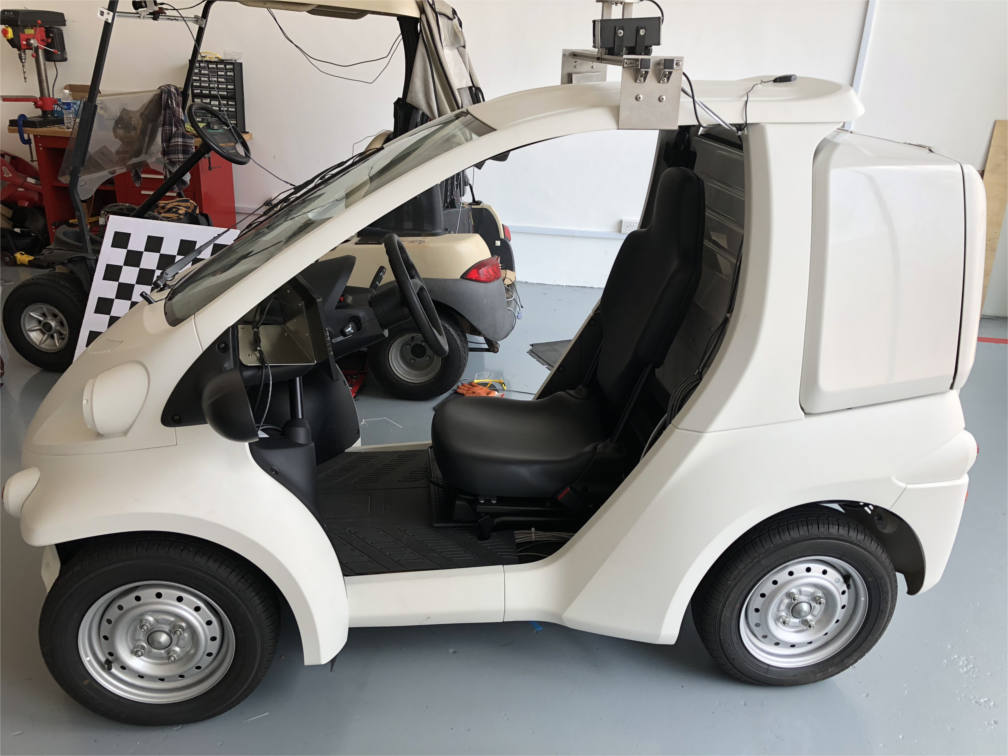
\includegraphics[width=0.8\textwidth]{singpilot.jpg}
  \end{figure}

\end{frame}

\begin{frame}{Localization of Autonomous Vehicles via Secure Sensor Fusion}
  \begin{columns}
    \begin{column}{0.48\textwidth}
      \begin{figure}
	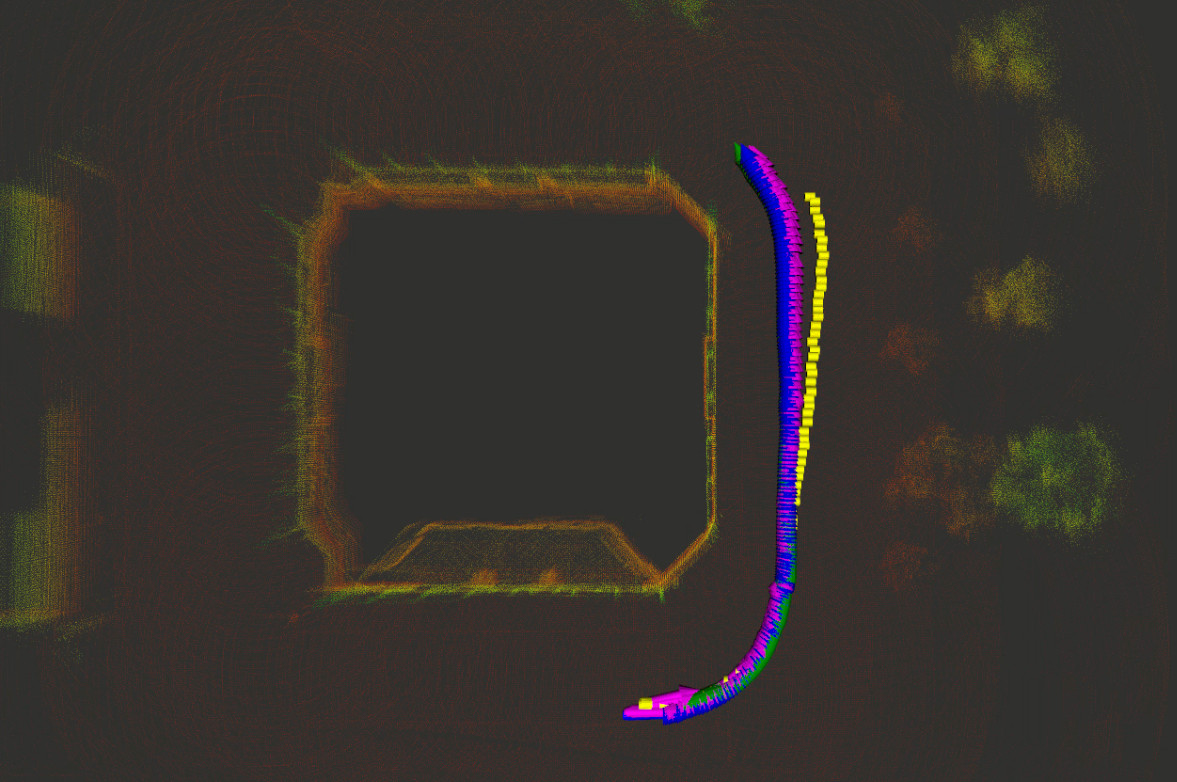
\includegraphics[width=\textwidth]{gnssdrift.jpg}
	\caption{EKF}
      \end{figure}
    \end{column}
    \begin{column}{0.48\textwidth} 		
      \begin{figure}
	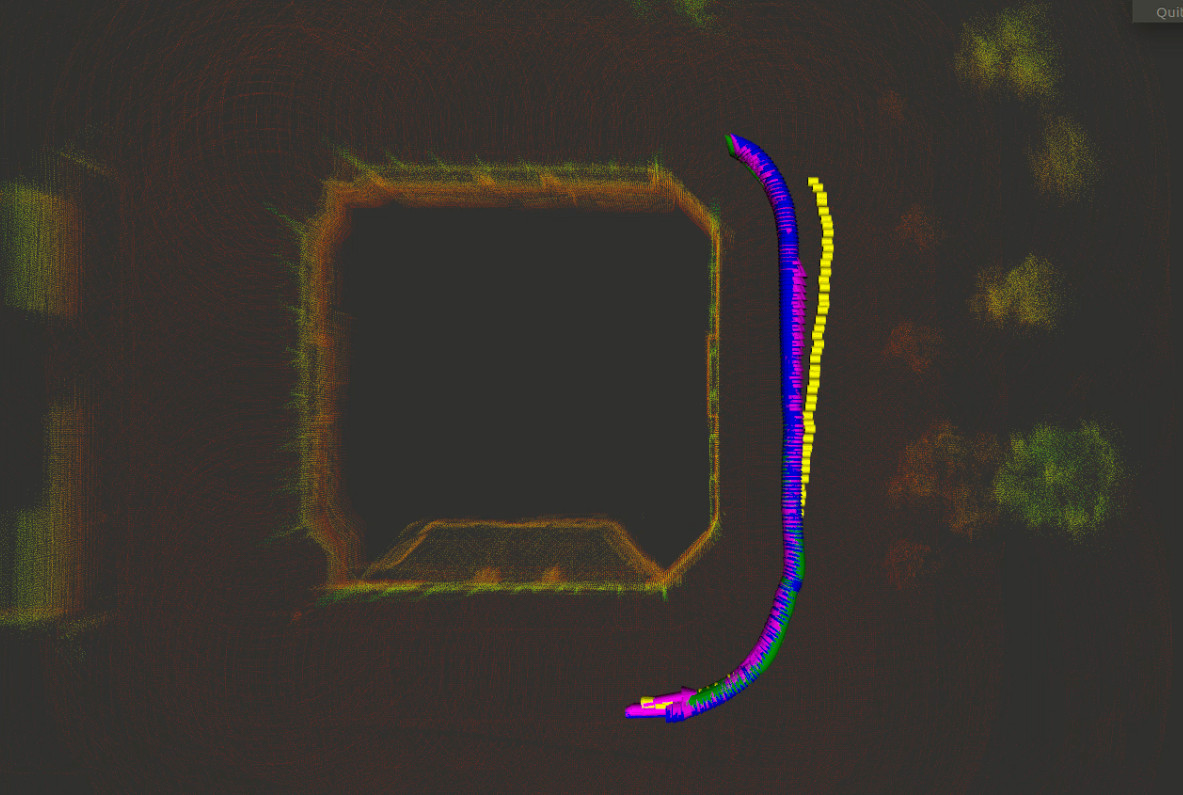
\includegraphics[width=\textwidth]{gnssdriftsafe.jpg}
	\caption{Secure EKF}
      \end{figure}
    \end{column}
  \end{columns}
\end{frame}


\section{Conclusion}

%\begin{frame}{Towards a Science of CPS Security}
%  \begin{itemize}
%    \item We consider both the static and dynamic state estimation problem in adversarial environment 
%    \item For static estimation, we propose a convex optimization based estimator and derive necessary and sufficient condition for its stability
%    \item For dynamic estimation, we propose a local filter + global fusion design:
%      \begin{enumerate}
%	\item In the absence of the attack, we recover the optimal Kalman filter with certain probabiliy
%	\item In the presence of the attack, we provide a sufficient condition for stability
%	\item For $A$ matrix whose unstable eigenvalues have geometric multiplicity of 1, the filter also achieves optimal security 
%      \end{enumerate}
%    \item Future directions: How to combine information security with system theory to provide defense in depth?
%  \end{itemize}
%\end{frame}
%
%\begin{frame}{Acknowledgement}
%  \begin{itemize}
%    \item Duo Han, Xinghua Liu, Zishuo Li
%    \item Lihua Xie, Emanuele Garone 
%    \item NTU Autonomous Driving Group: Danwei Wang, Jakub Tomasek, Qipeng Liu, Ehsan Mihankhah, Xiaoqiang Ren, Xiaoyu Mo 
%  \end{itemize}
%\end{frame}


\begin{frame}{Towards a Science of CPS Security}
  \begin{itemize}
  \item We consider intrusion detection problem in adversarial environment and propose an active detection scheme.
    \item We consider both the static and dynamic state estimation problem in adversarial environment 
    \item For static estimation, we propose a convex optimization based estimator and derive necessary and sufficient condition for its stability
  \item How to systematically design secure algorithms?
  \item How to combine information security with system theory to provide defense in depth?
  \end{itemize}
\end{frame}

\begin{frame}{Acknowledgement}
  \begin{itemize}
  \item Rohan Chabukswar, Sean Weerakkody, Hanxiao Liu, Jiaqi Yan, Zishuo Li
  \item Bruno Sinopoli, Lihua Xie, Karl H. Johansson
  \end{itemize}
\end{frame}

%\begin{frame}[allowframebreaks]
%     \printbibliography
%\end{frame} 

\begin{frame}[standout]
  感谢聆听!请各位老师批评指正
\end{frame}

\end{document}
